\documentclass[twoside]{book}

% Packages required by doxygen
\usepackage{calc}
\usepackage{doxygen}
\usepackage{graphicx}
\usepackage[utf8]{inputenc}
\usepackage{makeidx}
\usepackage{multicol}
\usepackage{multirow}
\usepackage{textcomp}
\usepackage[table]{xcolor}

% NLS support packages
\usepackage[ngerman]{babel}

% Font selection
\usepackage[T1]{fontenc}
\usepackage{mathptmx}
\usepackage[scaled=.90]{helvet}
\usepackage{courier}
\usepackage{amssymb}
\usepackage{sectsty}
\renewcommand{\familydefault}{\sfdefault}
\allsectionsfont{%
  \fontseries{bc}\selectfont%
  \color{darkgray}%
}
\renewcommand{\DoxyLabelFont}{%
  \fontseries{bc}\selectfont%
  \color{darkgray}%
}

% Page & text layout
\usepackage{geometry}
\geometry{%
  a4paper,%
  top=2.5cm,%
  bottom=2.5cm,%
  left=2.5cm,%
  right=2.5cm%
}
\tolerance=750
\hfuzz=15pt
\hbadness=750
\setlength{\emergencystretch}{15pt}
\setlength{\parindent}{0cm}
\setlength{\parskip}{0.2cm}
\makeatletter
\renewcommand{\paragraph}{%
  \@startsection{paragraph}{4}{0ex}{-1.0ex}{1.0ex}{%
    \normalfont\normalsize\bfseries\SS@parafont%
  }%
}
\renewcommand{\subparagraph}{%
  \@startsection{subparagraph}{5}{0ex}{-1.0ex}{1.0ex}{%
    \normalfont\normalsize\bfseries\SS@subparafont%
  }%
}
\makeatother

% Headers & footers
\usepackage{fancyhdr}
\pagestyle{fancyplain}
\fancyhead[LE]{\fancyplain{}{\bfseries\thepage}}
\fancyhead[CE]{\fancyplain{}{}}
\fancyhead[RE]{\fancyplain{}{\bfseries\leftmark}}
\fancyhead[LO]{\fancyplain{}{\bfseries\rightmark}}
\fancyhead[CO]{\fancyplain{}{}}
\fancyhead[RO]{\fancyplain{}{\bfseries\thepage}}
\fancyfoot[LE]{\fancyplain{}{}}
\fancyfoot[CE]{\fancyplain{}{}}
\fancyfoot[RE]{\fancyplain{}{\bfseries\scriptsize Erzeugt am Don Mär 24 2016 18\-:39\-:32 für Master-\/\-Slave von Doxygen }}
\fancyfoot[LO]{\fancyplain{}{\bfseries\scriptsize Erzeugt am Don Mär 24 2016 18\-:39\-:32 für Master-\/\-Slave von Doxygen }}
\fancyfoot[CO]{\fancyplain{}{}}
\fancyfoot[RO]{\fancyplain{}{}}
\renewcommand{\footrulewidth}{0.4pt}
\renewcommand{\chaptermark}[1]{%
  \markboth{#1}{}%
}
\renewcommand{\sectionmark}[1]{%
  \markright{\thesection\ #1}%
}

% Indices & bibliography
\usepackage{natbib}
\usepackage[titles]{tocloft}
\setcounter{tocdepth}{3}
\setcounter{secnumdepth}{5}
\makeindex

% Hyperlinks (required, but should be loaded last)
\usepackage{ifpdf}
\ifpdf
  \usepackage[pdftex,pagebackref=true]{hyperref}
\else
  \usepackage[ps2pdf,pagebackref=true]{hyperref}
\fi
\hypersetup{%
  colorlinks=true,%
  linkcolor=blue,%
  citecolor=blue,%
  unicode%
}

% Custom commands
\newcommand{\clearemptydoublepage}{%
  \newpage{\pagestyle{empty}\cleardoublepage}%
}


%===== C O N T E N T S =====

\begin{document}

% Titlepage & ToC
\hypersetup{pageanchor=false}
\pagenumbering{roman}
\begin{titlepage}
\vspace*{7cm}
\begin{center}%
{\Large Master-\/\-Slave }\\
\vspace*{1cm}
{\large Erzeugt von Doxygen 1.8.6}\\
\vspace*{0.5cm}
{\small Don Mär 24 2016 18:39:32}\\
\end{center}
\end{titlepage}
\clearemptydoublepage
\tableofcontents
\clearemptydoublepage
\pagenumbering{arabic}
\hypersetup{pageanchor=true}

%--- Begin generated contents ---
\chapter{Ausstehende Aufgaben}
\label{todo}
\hypertarget{todo}{}

\begin{DoxyRefList}
\item[\label{todo__todo000008}%
\hypertarget{todo__todo000008}{}%
Element \hyperlink{classGeometricKinematic_a2780149e9cc27767a216952be3c4efa1}{Geometric\-Kinematic\-:\-:get\-T\-\_\-0\-\_\-\-F\-L} ()]check ob noch benötigt \begin{DoxyReturn}{Rückgabe}

\end{DoxyReturn}

\item[\label{todo__todo000009}%
\hypertarget{todo__todo000009}{}%
Element \hyperlink{classGeometricKinematic_af17c2b463d3fa83ec26fb4b4d5abb64c}{Geometric\-Kinematic\-:\-:get\-T\-\_\-0\-\_\-\-Q4} ()]check ob noch benötigt \begin{DoxyReturn}{Rückgabe}

\end{DoxyReturn}

\item[\label{todo__todo000010}%
\hypertarget{todo__todo000010}{}%
Element \hyperlink{classGeometricKinematic_a985dc4eb67fb7989226d5b8d0ed2f9bf}{Geometric\-Kinematic\-:\-:set\-Angles} (const Eigen\-::\-Vector\-Xd value)]check ob noch benötigt, da jetzt über Services kommuniziert wird  
\item[\label{todo__todo000001}%
\hypertarget{todo__todo000001}{}%
Element \hyperlink{classGeometricKinematicCommander_afbfee50f578ff4098026413f41b916a3}{Geometric\-Kinematic\-Commander\-:\-:velocity\-\_\-} ]check ob noch benötigt  
\item[\label{todo__todo000002}%
\hypertarget{todo__todo000002}{}%
Element \hyperlink{classICommander_a01ec4010dc037bfb600cee7f0be9311c}{I\-Commander\-:\-:aperture\-Limit} ]löschen!  
\item[\label{todo__todo000006}%
\hypertarget{todo__todo000006}{}%
Element \hyperlink{classICommander_ab0d02021fcc73daaebcfe0a826e15f50}{I\-Commander\-:\-:bounding\-Box} ]Weitere Begrenzungsgeometrien einfügen und abstrakte Basisklasse einfügen  
\item[\label{todo__todo000004}%
\hypertarget{todo__todo000004}{}%
Element \hyperlink{classICommander_a038f78434eb525d73414c84624d3c3e4}{I\-Commander\-:\-:buttons} ]check ob noch benötigt \begin{DoxySeeAlso}{Siehe auch}
button\-Check  
\end{DoxySeeAlso}

\item[\label{todo__todo000003}%
\hypertarget{todo__todo000003}{}%
Element \hyperlink{classICommander_a166295c90210dae6c74e96d749c8ea1a}{I\-Commander\-:\-:height\-Safety} ]löschen!  
\item[\label{todo__todo000005}%
\hypertarget{todo__todo000005}{}%
Element \hyperlink{classICommander_a77d12525f98994352e2f2a450e04305b}{I\-Commander\-:\-:velocity\-Sub} ]check ob noch benötigt  
\item[\label{todo__todo000011}%
\hypertarget{todo__todo000011}{}%
Element \hyperlink{classIKinematic_a0f3ae85bd946533cf8a22120f597ab00}{I\-Kinematic\-:\-:T\-\_\-0\-\_\-\-Q4} ]Eindeutige Namenskonvention Q4tool und Q4lbr  
\item[\label{todo__todo000007}%
\hypertarget{todo__todo000007}{}%
Element \hyperlink{classNumericKinematicCommander_af12b3f3e1d3058dd7cf93b923ab6f13b}{Numeric\-Kinematic\-Commander\-:\-:lbr\-Joint\-Angles} ]check ob noch benötigt 
\end{DoxyRefList}
\chapter{Veraltete Elemente}
\label{deprecated}
\hypertarget{deprecated}{}

\begin{DoxyRefList}
\item[\label{deprecated__deprecated000002}%
\hypertarget{deprecated__deprecated000002}{}%
Element \hyperlink{classIKinematic_a5b70ed8f56334c0ee5041e5eb787a056}{I\-Kinematic\-:\-:aperture\-Max} ]
\item[\label{deprecated__deprecated000001}%
\hypertarget{deprecated__deprecated000001}{}%
Element \hyperlink{classIKinematic_a2c740366fa7cca713fb0962a6be7e9f0}{I\-Kinematic\-:\-:check\-T\-C\-P} (Eigen\-::\-Affine3d T\-C\-P)]wird in der neuen Version entfernt, da es eigene Überwachungsklassen gibt 
\begin{DoxyParams}{Parameter}
{\em T\-C\-P} & Aktueller T\-C\-P \\
\hline
\end{DoxyParams}
\begin{DoxyReturn}{Rückgabe}
Flag, ob der definierte Arbeitsraum eingehalten wurde 
\end{DoxyReturn}
\begin{DoxySeeAlso}{Siehe auch}
\hyperlink{classBoundingBox}{Bounding\-Box}  
\end{DoxySeeAlso}

\item[\label{deprecated__deprecated000003}%
\hypertarget{deprecated__deprecated000003}{}%
Element \hyperlink{classIKinematic_a628b36a0331179b979468468c1efed54}{I\-Kinematic\-:\-:penetration\-Max} ]
\item[\label{deprecated__deprecated000004}%
\hypertarget{deprecated__deprecated000004}{}%
Element \hyperlink{classIKinematic_a17905911cc852a855bd985bfda640ea2}{I\-Kinematic\-:\-:penetration\-Min} ]
\item[\label{deprecated__deprecated000005}%
\hypertarget{deprecated__deprecated000005}{}%
Element \hyperlink{classNumericKinematic_a6691d8d0fa2579cc4408acec0d2e864b}{Numeric\-Kinematic\-:\-:rescue\-Factor} ]
\end{DoxyRefList}
\chapter{Hierarchie-\/\-Verzeichnis}
\section{Klassenhierarchie}
Die Liste der Ableitungen ist -\/mit Einschränkungen-\/ alphabetisch sortiert\-:\begin{DoxyCompactList}
\item \contentsline{section}{Bounding\-Box}{\pageref{classBoundingBox}}{}
\item \contentsline{section}{Control\-Device}{\pageref{classControlDevice}}{}
\item \contentsline{section}{I\-Commander}{\pageref{classICommander}}{}
\begin{DoxyCompactList}
\item \contentsline{section}{Geometric\-Kinematic\-Commander}{\pageref{classGeometricKinematicCommander}}{}
\item \contentsline{section}{Numeric\-Kinematic\-Commander}{\pageref{classNumericKinematicCommander}}{}
\end{DoxyCompactList}
\item \contentsline{section}{I\-Kinematic}{\pageref{classIKinematic}}{}
\begin{DoxyCompactList}
\item \contentsline{section}{Geometric\-Kinematic}{\pageref{classGeometricKinematic}}{}
\item \contentsline{section}{Numeric\-Kinematic}{\pageref{classNumericKinematic}}{}
\end{DoxyCompactList}
\item \contentsline{section}{I\-Trajectory}{\pageref{classITrajectory}}{}
\begin{DoxyCompactList}
\item \contentsline{section}{Circle\-Trajectory}{\pageref{classCircleTrajectory}}{}
\item \contentsline{section}{Line\-Trajectory}{\pageref{classLineTrajectory}}{}
\item \contentsline{section}{P\-T\-P\-Trajectory}{\pageref{classPTPTrajectory}}{}
\end{DoxyCompactList}
\item \contentsline{section}{lbr\-Description\-Parameters}{\pageref{structlbrDescriptionParameters}}{}
\item \contentsline{section}{lbr\-Joint\-Angles}{\pageref{structlbrJointAngles}}{}
\item \contentsline{section}{Master\-Slave}{\pageref{classMasterSlave}}{}
\item \contentsline{section}{Master\-Slave\-Manipulation}{\pageref{classMasterSlaveManipulation}}{}
\item \contentsline{section}{Ros\-Open\-Igtl\-Bridge}{\pageref{classRosOpenIgtlBridge}}{}
\item \contentsline{section}{tool\-Angles}{\pageref{structtoolAngles}}{}
\item \contentsline{section}{tool\-Description\-Parameters}{\pageref{structtoolDescriptionParameters}}{}
\item \contentsline{section}{tool\-Motor\-Angles}{\pageref{structtoolMotorAngles}}{}
\item \contentsline{section}{Trajectory\-Generator}{\pageref{classTrajectoryGenerator}}{}
\end{DoxyCompactList}

\chapter{Klassen-\/\-Verzeichnis}
\section{Auflistung der Klassen}
Hier folgt die Aufzählung aller Klassen, Strukturen, Varianten und Schnittstellen mit einer Kurzbeschreibung\-:\begin{DoxyCompactList}
\item\contentsline{section}{\hyperlink{classBoundingBox}{Bounding\-Box} \\*Arbeitsraumbegrenzung in Form eines Quaders }{\pageref{classBoundingBox}}{}
\item\contentsline{section}{\hyperlink{classCircleTrajectory}{Circle\-Trajectory} \\*Klasse, die eine Interpolation einer Kreistrajektorie ermöglicht }{\pageref{classCircleTrajectory}}{}
\item\contentsline{section}{\hyperlink{classControlDevice}{Control\-Device} \\*Klasse zur Ansteuerung und Verwaltung verschiedener Low\-Level-\/\-Eingabegeräte, wie Game\-Pads oder dem Space\-Navigator }{\pageref{classControlDevice}}{}
\item\contentsline{section}{\hyperlink{classGeometricKinematic}{Geometric\-Kinematic} \\*Eine Klasse zur Berechnung der Kinematik des Werkzeuges und der Endeffektorlage des L\-B\-R iiwa }{\pageref{classGeometricKinematic}}{}
\item\contentsline{section}{\hyperlink{classGeometricKinematicCommander}{Geometric\-Kinematic\-Commander} \\*Klasse, die sich um die R\-O\-S-\/\-Kommunikation für die geometrisch bestimmte Kinematik kümmert }{\pageref{classGeometricKinematicCommander}}{}
\item\contentsline{section}{\hyperlink{classICommander}{I\-Commander} \\*Abstrakte Basisklasse zur Ansteuerung der beiden Kinematikmodelle über R\-O\-S }{\pageref{classICommander}}{}
\item\contentsline{section}{\hyperlink{classIKinematic}{I\-Kinematic} \\*Abstrakte Basisklasse für die Kinematikberechnung }{\pageref{classIKinematic}}{}
\item\contentsline{section}{\hyperlink{classITrajectory}{I\-Trajectory} \\*Abstrakte Basisklasse für verschiedene Trajektorienarten }{\pageref{classITrajectory}}{}
\item\contentsline{section}{\hyperlink{structlbrDescriptionParameters}{lbr\-Description\-Parameters} }{\pageref{structlbrDescriptionParameters}}{}
\item\contentsline{section}{\hyperlink{structlbrJointAngles}{lbr\-Joint\-Angles} }{\pageref{structlbrJointAngles}}{}
\item\contentsline{section}{\hyperlink{classLineTrajectory}{Line\-Trajectory} \\*Eine Klasse, die eine Interpolation eines Polynom fünften Grades zwischen zwei Punkten ermöglicht }{\pageref{classLineTrajectory}}{}
\item\contentsline{section}{\hyperlink{classMasterSlave}{Master\-Slave} }{\pageref{classMasterSlave}}{}
\item\contentsline{section}{\hyperlink{classMasterSlaveManipulation}{Master\-Slave\-Manipulation} \\*Klasse, die sich um die Manipulation des T\-C\-P mittels des Eingabegerätes kümmert }{\pageref{classMasterSlaveManipulation}}{}
\item\contentsline{section}{\hyperlink{classNumericKinematic}{Numeric\-Kinematic} \\*Klasse zur Berechnung der Kinematiken des Gesamtsystems mit 10 Achsen. Die inverse Kinematik wird numerisch mittels eines Least-\/\-Square-\/\-Problems gelöst Die Klasse berechnet die direkte und inverse Kinematik eines Gesamtsystems bestehend aus L\-B\-R iiwa und dem Laparoskop. Es besitzt insgesamt 10 Achsen, da der Trokarpunkt eingehalten werden muss, bleibt noch eine Redundanz mit Dimension 2 zur Optimierung der Gelenkwinkelkonfiguration. Diese können mit verschiedenen Optimierungskriterien, wie Singularitätsvermeidung, Kollisionsvermeidung, Geschwindigkeits-\/ und Beschleunigungsminimierung, sowie einer Winkelwächterfunktion parametriert werden Zum Lösen wird der Algorithmus aus Quad\-Prog++ eingesetzt, der auf die Eigen-\/\-Bibliothek umgeschrieben wurde }{\pageref{classNumericKinematic}}{}
\item\contentsline{section}{\hyperlink{classNumericKinematicCommander}{Numeric\-Kinematic\-Commander} \\*Klasse, die sich um die R\-O\-S-\/\-Kommunikation für die numerisch bestimmte Kinematik kümmert }{\pageref{classNumericKinematicCommander}}{}
\item\contentsline{section}{\hyperlink{classPTPTrajectory}{P\-T\-P\-Trajectory} }{\pageref{classPTPTrajectory}}{}
\item\contentsline{section}{\hyperlink{classRosOpenIgtlBridge}{Ros\-Open\-Igtl\-Bridge} \\*Eine R\-O\-S-\/\-Node zur Kommunikation zwischen R\-O\-S und dem L\-B\-R iiwa, welche über das Open\-I\-G\-T\-Link-\/\-Protokoll durchgeführt }{\pageref{classRosOpenIgtlBridge}}{}
\item\contentsline{section}{\hyperlink{structtoolAngles}{tool\-Angles} }{\pageref{structtoolAngles}}{}
\item\contentsline{section}{\hyperlink{structtoolDescriptionParameters}{tool\-Description\-Parameters} }{\pageref{structtoolDescriptionParameters}}{}
\item\contentsline{section}{\hyperlink{structtoolMotorAngles}{tool\-Motor\-Angles} }{\pageref{structtoolMotorAngles}}{}
\item\contentsline{section}{\hyperlink{classTrajectoryGenerator}{Trajectory\-Generator} \\*Klasse zum Abfahren verschiedener Trajektorien zur quantitativen Bestimmung des Trokarpunktes }{\pageref{classTrajectoryGenerator}}{}
\end{DoxyCompactList}

\chapter{Datei-\/\-Verzeichnis}
\section{Auflistung der Dateien}
Hier folgt die Aufzählung aller dokumentierten Dateien mit einer Kurzbeschreibung\-:\begin{DoxyCompactList}
\item\contentsline{section}{include/masterslave/\hyperlink{ControlDevice_8h}{Control\-Device.\-h} }{\pageref{ControlDevice_8h}}{}
\item\contentsline{section}{include/masterslave/{\bfseries Description\-Parameters.\-h} }{\pageref{DescriptionParameters_8h}}{}
\item\contentsline{section}{include/masterslave/{\bfseries Master\-Slave.\-h} }{\pageref{MasterSlave_8h}}{}
\item\contentsline{section}{include/masterslave/{\bfseries Open\-I\-G\-T\-L\-State\-Description.\-h} }{\pageref{OpenIGTLStateDescription_8h}}{}
\item\contentsline{section}{include/masterslave/\hyperlink{RosOpenIGTLBridge_8h}{Ros\-Open\-I\-G\-T\-L\-Bridge.\-h} }{\pageref{RosOpenIGTLBridge_8h}}{}
\item\contentsline{section}{include/masterslave/commander/\hyperlink{BoundingBox_8h}{Bounding\-Box.\-h} }{\pageref{BoundingBox_8h}}{}
\item\contentsline{section}{include/masterslave/commander/\hyperlink{GeometricKinematicCommander_8h}{Geometric\-Kinematic\-Commander.\-h} }{\pageref{GeometricKinematicCommander_8h}}{}
\item\contentsline{section}{include/masterslave/commander/\hyperlink{ICommander_8h}{I\-Commander.\-h} }{\pageref{ICommander_8h}}{}
\item\contentsline{section}{include/masterslave/commander/\hyperlink{NumericKinematicCommander_8h}{Numeric\-Kinematic\-Commander.\-h} }{\pageref{NumericKinematicCommander_8h}}{}
\item\contentsline{section}{include/masterslave/kinematic/\hyperlink{GeometricKinematic_8h}{Geometric\-Kinematic.\-h} }{\pageref{GeometricKinematic_8h}}{}
\item\contentsline{section}{include/masterslave/kinematic/\hyperlink{IKinematic_8h}{I\-Kinematic.\-h} }{\pageref{IKinematic_8h}}{}
\item\contentsline{section}{include/masterslave/kinematic/\hyperlink{NumericKinematic_8h}{Numeric\-Kinematic.\-h} }{\pageref{NumericKinematic_8h}}{}
\item\contentsline{section}{include/masterslave/manipulation/\hyperlink{MasterSlaveManipulation_8h}{Master\-Slave\-Manipulation.\-h} }{\pageref{MasterSlaveManipulation_8h}}{}
\item\contentsline{section}{include/masterslave/manipulation/\hyperlink{TrajectoryGenerator_8h}{Trajectory\-Generator.\-h} }{\pageref{TrajectoryGenerator_8h}}{}
\item\contentsline{section}{include/masterslave/manipulation/trajectory/\hyperlink{CircleTrajectory_8h}{Circle\-Trajectory.\-h} }{\pageref{CircleTrajectory_8h}}{}
\item\contentsline{section}{include/masterslave/manipulation/trajectory/\hyperlink{ITrajectory_8h}{I\-Trajectory.\-h} }{\pageref{ITrajectory_8h}}{}
\item\contentsline{section}{include/masterslave/manipulation/trajectory/\hyperlink{LineTrajectory_8h}{Line\-Trajectory.\-h} }{\pageref{LineTrajectory_8h}}{}
\item\contentsline{section}{include/masterslave/manipulation/trajectory/{\bfseries P\-T\-P\-Trajectory.\-h} }{\pageref{PTPTrajectory_8h}}{}
\item\contentsline{section}{include/masterslave/optimization/{\bfseries eiquadprog.\-hpp} }{\pageref{eiquadprog_8hpp}}{}
\end{DoxyCompactList}

\chapter{Klassen-\/\-Dokumentation}
\hypertarget{classBoundingBox}{\section{Bounding\-Box Klassenreferenz}
\label{classBoundingBox}\index{Bounding\-Box@{Bounding\-Box}}
}


Arbeitsraumbegrenzung in Form eines Quaders.  




{\ttfamily \#include $<$Bounding\-Box.\-h$>$}



Zusammengehörigkeiten von Bounding\-Box\-:
\nopagebreak
\begin{figure}[H]
\begin{center}
\leavevmode
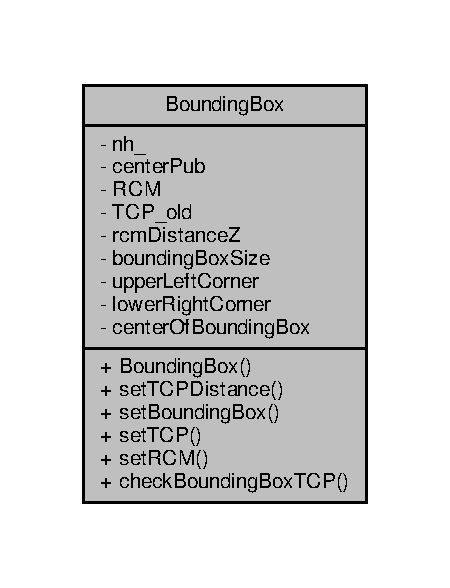
\includegraphics[width=216pt]{classBoundingBox__coll__graph}
\end{center}
\end{figure}
\subsection*{Öffentliche Methoden}
\begin{DoxyCompactItemize}
\item 
\hypertarget{classBoundingBox_a9cca955ede84d4eacb28867bab60515a}{{\bfseries Bounding\-Box} (ros\-::\-Node\-Handle \&nh, Eigen\-::\-Affine3d T\-C\-P, Eigen\-::\-Vector3d Remote\-Center\-Of\-Motion, Eigen\-::\-Vector3d bounding\-Box\-Size\-Vector, double rcm\-Distance)}\label{classBoundingBox_a9cca955ede84d4eacb28867bab60515a}

\item 
\hypertarget{classBoundingBox_a77311a3a943fc60baafcdb2736b72dd1}{void {\bfseries set\-T\-C\-P\-Distance} (double value)}\label{classBoundingBox_a77311a3a943fc60baafcdb2736b72dd1}

\item 
\hypertarget{classBoundingBox_a8876f5598dd64840cecb62876880a672}{void {\bfseries set\-Bounding\-Box} (Eigen\-::\-Vector3d value)}\label{classBoundingBox_a8876f5598dd64840cecb62876880a672}

\item 
\hypertarget{classBoundingBox_a90fa5d3bf50542bec97dff5a8cc5ea96}{void {\bfseries set\-T\-C\-P} (Eigen\-::\-Affine3d T\-C\-P)}\label{classBoundingBox_a90fa5d3bf50542bec97dff5a8cc5ea96}

\item 
\hypertarget{classBoundingBox_ace45e8101d411b6afe423ad2f919b733}{void {\bfseries set\-R\-C\-M} (Eigen\-::\-Vector3d remote\-Center\-Of\-Motion)}\label{classBoundingBox_ace45e8101d411b6afe423ad2f919b733}

\item 
bool \hyperlink{classBoundingBox_ad5ea0824f81b82172ac870b344e26369}{check\-Bounding\-Box\-T\-C\-P} (Eigen\-::\-Affine3d T\-C\-P)
\begin{DoxyCompactList}\small\item\em Überprüft, ob der T\-C\-P außerhalb des erlaubten Arbeitsraumes liegt. \end{DoxyCompactList}\end{DoxyCompactItemize}
\subsection*{Private Attribute}
\begin{DoxyCompactItemize}
\item 
\hypertarget{classBoundingBox_ac9681b03b7864b0cbc2537f643ce007d}{ros\-::\-Node\-Handle {\bfseries nh\-\_\-}}\label{classBoundingBox_ac9681b03b7864b0cbc2537f643ce007d}

\item 
\hypertarget{classBoundingBox_aa4451c8bf589cd4a549be53756bd0ae8}{ros\-::\-Publisher \hyperlink{classBoundingBox_aa4451c8bf589cd4a549be53756bd0ae8}{center\-Pub}}\label{classBoundingBox_aa4451c8bf589cd4a549be53756bd0ae8}

\begin{DoxyCompactList}\small\item\em Sender in R\-O\-S, um in V-\/\-Rep den Quader an der richtigen Stelle anzuzeigen. \end{DoxyCompactList}\item 
\hypertarget{classBoundingBox_a1aefa364b31d2a36fce50b79edbb1116}{Eigen\-::\-Vector3d \hyperlink{classBoundingBox_a1aefa364b31d2a36fce50b79edbb1116}{R\-C\-M}}\label{classBoundingBox_a1aefa364b31d2a36fce50b79edbb1116}

\begin{DoxyCompactList}\small\item\em Koordinaten des Trokarpunktes. \end{DoxyCompactList}\item 
\hypertarget{classBoundingBox_a4cc474bf1d1ec1c50fa403e33ac385f1}{Eigen\-::\-Affine3d \hyperlink{classBoundingBox_a4cc474bf1d1ec1c50fa403e33ac385f1}{T\-C\-P\-\_\-old}}\label{classBoundingBox_a4cc474bf1d1ec1c50fa403e33ac385f1}

\begin{DoxyCompactList}\small\item\em alter T\-C\-P \end{DoxyCompactList}\item 
\hypertarget{classBoundingBox_a3ea0aa423615b74d9244c94fb7a33870}{double \hyperlink{classBoundingBox_a3ea0aa423615b74d9244c94fb7a33870}{rcm\-Distance\-Z}}\label{classBoundingBox_a3ea0aa423615b74d9244c94fb7a33870}

\begin{DoxyCompactList}\small\item\em Abstand in z-\/\-Richtung zwischen dem Trokarpunkt und der Oberseite des Quaders. \end{DoxyCompactList}\item 
\hypertarget{classBoundingBox_a0331404e2b255f97beba34733d15f52e}{Eigen\-::\-Vector3d \hyperlink{classBoundingBox_a0331404e2b255f97beba34733d15f52e}{bounding\-Box\-Size}}\label{classBoundingBox_a0331404e2b255f97beba34733d15f52e}

\begin{DoxyCompactList}\small\item\em Größe des Quaders in drei Dimensionen. \end{DoxyCompactList}\item 
\hypertarget{classBoundingBox_a3acf7f8c01012c872b0911fe74c50880}{Eigen\-::\-Vector3d \hyperlink{classBoundingBox_a3acf7f8c01012c872b0911fe74c50880}{upper\-Left\-Corner}}\label{classBoundingBox_a3acf7f8c01012c872b0911fe74c50880}

\begin{DoxyCompactList}\small\item\em Koordinaten der oberen linken Ecke des Quaders. \end{DoxyCompactList}\item 
\hypertarget{classBoundingBox_a961e24b17d0ae9a404790bebfbf0ad02}{Eigen\-::\-Vector3d \hyperlink{classBoundingBox_a961e24b17d0ae9a404790bebfbf0ad02}{lower\-Right\-Corner}}\label{classBoundingBox_a961e24b17d0ae9a404790bebfbf0ad02}

\begin{DoxyCompactList}\small\item\em Koordinaten er linken unteren Ecke des Quaders. \end{DoxyCompactList}\item 
\hypertarget{classBoundingBox_a7ec70c3bac170b64ce2bac40f14f21c7}{Eigen\-::\-Vector3d \hyperlink{classBoundingBox_a7ec70c3bac170b64ce2bac40f14f21c7}{center\-Of\-Bounding\-Box}}\label{classBoundingBox_a7ec70c3bac170b64ce2bac40f14f21c7}

\begin{DoxyCompactList}\small\item\em Zentroid des Quaders. \end{DoxyCompactList}\end{DoxyCompactItemize}


\subsection{Ausführliche Beschreibung}
Arbeitsraumbegrenzung in Form eines Quaders. 

\begin{DoxyAuthor}{Autor}
Fabian Baier 
\end{DoxyAuthor}
\begin{DoxyDate}{Datum}
19.\-03.\-2016 
\end{DoxyDate}


\subsection{Dokumentation der Elementfunktionen}
\hypertarget{classBoundingBox_ad5ea0824f81b82172ac870b344e26369}{\index{Bounding\-Box@{Bounding\-Box}!check\-Bounding\-Box\-T\-C\-P@{check\-Bounding\-Box\-T\-C\-P}}
\index{check\-Bounding\-Box\-T\-C\-P@{check\-Bounding\-Box\-T\-C\-P}!BoundingBox@{Bounding\-Box}}
\subsubsection[{check\-Bounding\-Box\-T\-C\-P}]{\setlength{\rightskip}{0pt plus 5cm}Bounding\-Box\-::check\-Bounding\-Box\-T\-C\-P (
\begin{DoxyParamCaption}
\item[{Eigen\-::\-Affine3d}]{T\-C\-P}
\end{DoxyParamCaption}
)}}\label{classBoundingBox_ad5ea0824f81b82172ac870b344e26369}


Überprüft, ob der T\-C\-P außerhalb des erlaubten Arbeitsraumes liegt. 


\begin{DoxyParams}{Parameter}
{\em T\-C\-P} & aktueller T\-C\-P \\
\hline
\end{DoxyParams}
\begin{DoxyReturn}{Rückgabe}
Flag, ob der T\-C\-P im erlaubten Arbeitsraum liegt 
\end{DoxyReturn}


Die Dokumentation für diese Klasse wurde erzeugt aufgrund der Datei\-:\begin{DoxyCompactItemize}
\item 
include/masterslave/commander/\hyperlink{BoundingBox_8h}{Bounding\-Box.\-h}\end{DoxyCompactItemize}

\hypertarget{classCircleTrajectory}{\section{Circle\-Trajectory Klassenreferenz}
\label{classCircleTrajectory}\index{Circle\-Trajectory@{Circle\-Trajectory}}
}


Klasse, die eine Interpolation einer Kreistrajektorie ermöglicht.  




{\ttfamily \#include $<$Circle\-Trajectory.\-h$>$}



Klassendiagramm für Circle\-Trajectory\-:
\nopagebreak
\begin{figure}[H]
\begin{center}
\leavevmode
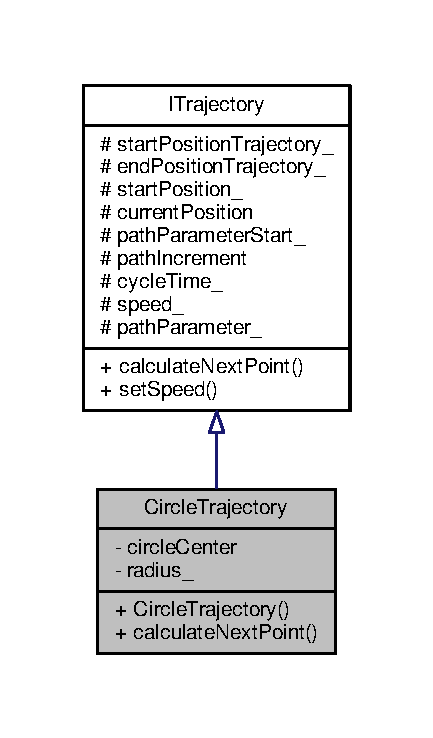
\includegraphics[width=208pt]{classCircleTrajectory__inherit__graph}
\end{center}
\end{figure}


Zusammengehörigkeiten von Circle\-Trajectory\-:
\nopagebreak
\begin{figure}[H]
\begin{center}
\leavevmode
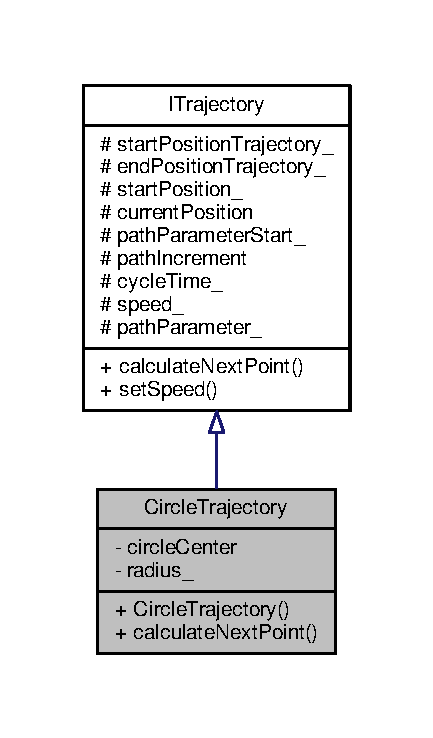
\includegraphics[width=208pt]{classCircleTrajectory__coll__graph}
\end{center}
\end{figure}
\subsection*{Öffentliche Methoden}
\begin{DoxyCompactItemize}
\item 
\hypertarget{classCircleTrajectory_a4d8e3dad20e722dd795ddba29eaea785}{{\bfseries Circle\-Trajectory} (Eigen\-::\-Affine3d start\-Point, Eigen\-::\-Vector3d R\-C\-M, double radius, double z\-Coord, double speed, double cycle\-Time)}\label{classCircleTrajectory_a4d8e3dad20e722dd795ddba29eaea785}

\item 
Eigen\-::\-Affine3d \hyperlink{classCircleTrajectory_a5629eff71ee01458eb8cdf7ad2b4b82f}{calculate\-Next\-Point} ()
\end{DoxyCompactItemize}
\subsection*{Private Attribute}
\begin{DoxyCompactItemize}
\item 
\hypertarget{classCircleTrajectory_a4e09c5712c0944044fcba484c8ebbfeb}{Eigen\-::\-Affine3d \hyperlink{classCircleTrajectory_a4e09c5712c0944044fcba484c8ebbfeb}{circle\-Center}}\label{classCircleTrajectory_a4e09c5712c0944044fcba484c8ebbfeb}

\begin{DoxyCompactList}\small\item\em Zentroid der Kreistrajektorie. \end{DoxyCompactList}\item 
\hypertarget{classCircleTrajectory_adcf4904d1d0fbb68773745aa7cd32621}{double \hyperlink{classCircleTrajectory_adcf4904d1d0fbb68773745aa7cd32621}{radius\-\_\-}}\label{classCircleTrajectory_adcf4904d1d0fbb68773745aa7cd32621}

\begin{DoxyCompactList}\small\item\em Radius der Kreistrajektorie. \end{DoxyCompactList}\end{DoxyCompactItemize}
\subsection*{Weitere Geerbte Elemente}


\subsection{Ausführliche Beschreibung}
Klasse, die eine Interpolation einer Kreistrajektorie ermöglicht. 

\begin{DoxyAuthor}{Autor}
Fabian Baier 
\end{DoxyAuthor}
\begin{DoxyDate}{Datum}
20.\-03.\-2016 
\end{DoxyDate}


\subsection{Dokumentation der Elementfunktionen}
\hypertarget{classCircleTrajectory_a5629eff71ee01458eb8cdf7ad2b4b82f}{\index{Circle\-Trajectory@{Circle\-Trajectory}!calculate\-Next\-Point@{calculate\-Next\-Point}}
\index{calculate\-Next\-Point@{calculate\-Next\-Point}!CircleTrajectory@{Circle\-Trajectory}}
\subsubsection[{calculate\-Next\-Point}]{\setlength{\rightskip}{0pt plus 5cm}Circle\-Trajectory\-::calculate\-Next\-Point (
\begin{DoxyParamCaption}
{}
\end{DoxyParamCaption}
)\hspace{0.3cm}{\ttfamily [virtual]}}}\label{classCircleTrajectory_a5629eff71ee01458eb8cdf7ad2b4b82f}
\begin{DoxySeeAlso}{Siehe auch}
\hyperlink{classITrajectory}{I\-Trajectory} 
\end{DoxySeeAlso}


Implementiert \hyperlink{classITrajectory_a7baff9fb2fc20987e9469d736a90406b}{I\-Trajectory}.



Die Dokumentation für diese Klasse wurde erzeugt aufgrund der Datei\-:\begin{DoxyCompactItemize}
\item 
include/masterslave/manipulation/trajectory/\hyperlink{CircleTrajectory_8h}{Circle\-Trajectory.\-h}\end{DoxyCompactItemize}

\hypertarget{classControlDevice}{\section{Control\-Device Klassenreferenz}
\label{classControlDevice}\index{Control\-Device@{Control\-Device}}
}


Klasse zur Ansteuerung und Verwaltung verschiedener Low\-Level-\/\-Eingabegeräte, wie Game\-Pads oder dem Space\-Navigator.  




{\ttfamily \#include $<$Control\-Device.\-h$>$}



Zusammengehörigkeiten von Control\-Device\-:
\nopagebreak
\begin{figure}[H]
\begin{center}
\leavevmode
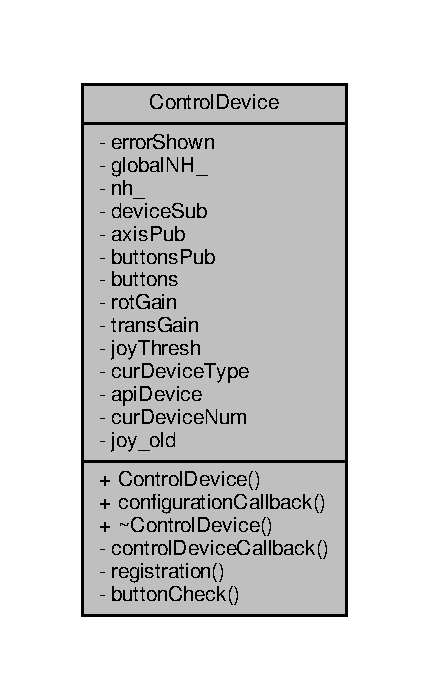
\includegraphics[width=206pt]{classControlDevice__coll__graph}
\end{center}
\end{figure}
\subsection*{Öffentliche Methoden}
\begin{DoxyCompactItemize}
\item 
\hypertarget{classControlDevice_ae28b973d924a233a70275dedc640d430}{{\bfseries Control\-Device} (ros\-::\-Node\-Handle \&nh)}\label{classControlDevice_ae28b973d924a233a70275dedc640d430}

\item 
void \hyperlink{classControlDevice_afc4d912d844cd888f87414bca1b68aa6}{configuration\-Callback} (masterslave\-::\-Control\-Device\-Config \&config, uint32\-\_\-t level)
\begin{DoxyCompactList}\small\item\em dynamic reconfigure Callback Methode \end{DoxyCompactList}\end{DoxyCompactItemize}
\subsection*{Private Methoden}
\begin{DoxyCompactItemize}
\item 
void \hyperlink{classControlDevice_a30fb0b63f5807af4c0c27b3e3dd837e8}{control\-Device\-Callback} (const sensor\-\_\-msgs\-::\-Joy\-::\-Const\-Ptr \&joy)
\begin{DoxyCompactList}\small\item\em Callback-\/\-Methode für die Eigabegeräte bzw. deren Achsen und Knöpfe. \end{DoxyCompactList}\item 
\hypertarget{classControlDevice_a54555a7b2c3913f4401839d66d6434c4}{void \hyperlink{classControlDevice_a54555a7b2c3913f4401839d66d6434c4}{registration} ()}\label{classControlDevice_a54555a7b2c3913f4401839d66d6434c4}

\begin{DoxyCompactList}\small\item\em Registrierung des Eingabegerätes mit Informationen des Parameterserver. \end{DoxyCompactList}\item 
\hypertarget{classControlDevice_a461ef41cef8de1e7c0a0877a260f8a1b}{void \hyperlink{classControlDevice_a461ef41cef8de1e7c0a0877a260f8a1b}{button\-Check} ()}\label{classControlDevice_a461ef41cef8de1e7c0a0877a260f8a1b}

\begin{DoxyCompactList}\small\item\em Festlegung der Knopfbelegung. \end{DoxyCompactList}\end{DoxyCompactItemize}
\subsection*{Private Attribute}
\begin{DoxyCompactItemize}
\item 
\hypertarget{classControlDevice_af75949ecac8c9f77d8d972e17fab6fce}{bool \hyperlink{classControlDevice_af75949ecac8c9f77d8d972e17fab6fce}{error\-Shown}}\label{classControlDevice_af75949ecac8c9f77d8d972e17fab6fce}

\begin{DoxyCompactList}\small\item\em Flag, welches anzeigt, ob der \char`\"{}\-Kein-\/\-Eingabegerät\char`\"{}-\/\-Fehler bereits gezeigt wird. \end{DoxyCompactList}\item 
\hypertarget{classControlDevice_a757158b73df10bde260ff29734048465}{ros\-::\-Node\-Handle {\bfseries global\-N\-H\-\_\-}}\label{classControlDevice_a757158b73df10bde260ff29734048465}

\item 
\hypertarget{classControlDevice_ad19d5025e89e12b827b32a086e2b0763}{ros\-::\-Node\-Handle {\bfseries nh\-\_\-}}\label{classControlDevice_ad19d5025e89e12b827b32a086e2b0763}

\item 
\hypertarget{classControlDevice_ae8f236385e5bc7d4286d40cf6d6c5049}{ros\-::\-Subscriber \hyperlink{classControlDevice_ae8f236385e5bc7d4286d40cf6d6c5049}{device\-Sub}}\label{classControlDevice_ae8f236385e5bc7d4286d40cf6d6c5049}

\begin{DoxyCompactList}\small\item\em Empfänger in R\-O\-S, der die Daten der Eingabegeräte empfängt. \end{DoxyCompactList}\item 
\hypertarget{classControlDevice_ac7336bd3dae7b371b118d04086ab1b4b}{ros\-::\-Publisher \hyperlink{classControlDevice_ac7336bd3dae7b371b118d04086ab1b4b}{axis\-Pub}}\label{classControlDevice_ac7336bd3dae7b371b118d04086ab1b4b}

\begin{DoxyCompactList}\small\item\em Sender in R\-O\-S, der die gefilterten und skalierten Achswerte weitersendet. \end{DoxyCompactList}\item 
\hypertarget{classControlDevice_a9f35eb488a8e73d6a48a1d45f82c6979}{ros\-::\-Publisher \hyperlink{classControlDevice_a9f35eb488a8e73d6a48a1d45f82c6979}{buttons\-Pub}}\label{classControlDevice_a9f35eb488a8e73d6a48a1d45f82c6979}

\begin{DoxyCompactList}\small\item\em Sender in R\-O\-S, der die Knöpfe sendet. \end{DoxyCompactList}\item 
\hypertarget{classControlDevice_ae08a1b61bf2c58f3248ddbd0e57904c9}{std\-::map$<$ int, std\-::string $>$ \hyperlink{classControlDevice_ae08a1b61bf2c58f3248ddbd0e57904c9}{buttons}}\label{classControlDevice_ae08a1b61bf2c58f3248ddbd0e57904c9}

\begin{DoxyCompactList}\small\item\em Buttons und Funktionen sind in dieser Map verknüpft. \end{DoxyCompactList}\item 
\hypertarget{classControlDevice_aee18bd1109d4220e3ede5a47bdc3aa5a}{double {\bfseries rot\-Gain}}\label{classControlDevice_aee18bd1109d4220e3ede5a47bdc3aa5a}

\item 
\hypertarget{classControlDevice_a51812d84ab5cce6233d296fc8e0d000e}{double \hyperlink{classControlDevice_a51812d84ab5cce6233d296fc8e0d000e}{trans\-Gain}}\label{classControlDevice_a51812d84ab5cce6233d296fc8e0d000e}

\begin{DoxyCompactList}\small\item\em Verstärkungen für die Rotations-\/ und Translationsachsen. \end{DoxyCompactList}\item 
\hypertarget{classControlDevice_a10e97555607f3140b31b14458dc23352}{double \hyperlink{classControlDevice_a10e97555607f3140b31b14458dc23352}{joy\-Thresh}}\label{classControlDevice_a10e97555607f3140b31b14458dc23352}

\begin{DoxyCompactList}\small\item\em Schwellwert für die Joystickachsen. \end{DoxyCompactList}\item 
\hypertarget{classControlDevice_af353f21c18ff47eb33f9331e8b7263c5}{std\-::string \hyperlink{classControlDevice_af353f21c18ff47eb33f9331e8b7263c5}{cur\-Device\-Type}}\label{classControlDevice_af353f21c18ff47eb33f9331e8b7263c5}

\begin{DoxyCompactList}\small\item\em aktueller Eingabegerätetyp (G\-A\-M\-E\-P\-A\-D, S\-P\-A\-C\-E\-N\-A\-V) \end{DoxyCompactList}\item 
\hypertarget{classControlDevice_aaf8698d8be6563f2d0833a42375e8aed}{std\-::string {\bfseries api\-Device}}\label{classControlDevice_aaf8698d8be6563f2d0833a42375e8aed}

\item 
\hypertarget{classControlDevice_ad7ad0a10221a0dc54bd3c723d56a9cb8}{int {\bfseries cur\-Device\-Num}}\label{classControlDevice_ad7ad0a10221a0dc54bd3c723d56a9cb8}

\item 
\hypertarget{classControlDevice_a2198a9a7b72b39c65a6f025db61e2108}{sensor\-\_\-msgs\-::\-Joy \hyperlink{classControlDevice_a2198a9a7b72b39c65a6f025db61e2108}{joy\-\_\-old}}\label{classControlDevice_a2198a9a7b72b39c65a6f025db61e2108}

\begin{DoxyCompactList}\small\item\em Joystickachswerte des letzten Zyklus, um Änderungen detektieren zu können. \end{DoxyCompactList}\end{DoxyCompactItemize}


\subsection{Ausführliche Beschreibung}
Klasse zur Ansteuerung und Verwaltung verschiedener Low\-Level-\/\-Eingabegeräte, wie Game\-Pads oder dem Space\-Navigator. 

\begin{DoxyAuthor}{Autor}
Fabian Baier 
\end{DoxyAuthor}
\begin{DoxyDate}{Datum}
19.\-03.\-2016
\end{DoxyDate}
\begin{DoxyVersion}{Version}
0.\-2 
\end{DoxyVersion}


\subsection{Dokumentation der Elementfunktionen}
\hypertarget{classControlDevice_afc4d912d844cd888f87414bca1b68aa6}{\index{Control\-Device@{Control\-Device}!configuration\-Callback@{configuration\-Callback}}
\index{configuration\-Callback@{configuration\-Callback}!ControlDevice@{Control\-Device}}
\subsubsection[{configuration\-Callback}]{\setlength{\rightskip}{0pt plus 5cm}void Control\-Device\-::configuration\-Callback (
\begin{DoxyParamCaption}
\item[{masterslave\-::\-Control\-Device\-Config \&}]{config, }
\item[{uint32\-\_\-t}]{level}
\end{DoxyParamCaption}
)}}\label{classControlDevice_afc4d912d844cd888f87414bca1b68aa6}


dynamic reconfigure Callback Methode 


\begin{DoxyParams}{Parameter}
{\em config} & Konfiguration für verschiedene Filterlevel und Verstärkungsfaktoren \\
\hline
{\em level} & Bitmaske um Einstellungen zu maskieren \\
\hline
\end{DoxyParams}
\begin{DoxySeeAlso}{Siehe auch}
Control\-Device.\-cfg 
\end{DoxySeeAlso}
\hypertarget{classControlDevice_a30fb0b63f5807af4c0c27b3e3dd837e8}{\index{Control\-Device@{Control\-Device}!control\-Device\-Callback@{control\-Device\-Callback}}
\index{control\-Device\-Callback@{control\-Device\-Callback}!ControlDevice@{Control\-Device}}
\subsubsection[{control\-Device\-Callback}]{\setlength{\rightskip}{0pt plus 5cm}Control\-Device\-::control\-Device\-Callback (
\begin{DoxyParamCaption}
\item[{const sensor\-\_\-msgs\-::\-Joy\-::\-Const\-Ptr \&}]{joy}
\end{DoxyParamCaption}
)\hspace{0.3cm}{\ttfamily [private]}}}\label{classControlDevice_a30fb0b63f5807af4c0c27b3e3dd837e8}


Callback-\/\-Methode für die Eigabegeräte bzw. deren Achsen und Knöpfe. 


\begin{DoxyParams}{Parameter}
{\em joy} & Achs-\/ und Knopfvektoren des jeweiligen Eingabegeräts \\
\hline
\end{DoxyParams}


Die Dokumentation für diese Klasse wurde erzeugt aufgrund der Datei\-:\begin{DoxyCompactItemize}
\item 
include/masterslave/\hyperlink{ControlDevice_8h}{Control\-Device.\-h}\end{DoxyCompactItemize}

\hypertarget{classGeometricKinematic}{\section{Geometric\-Kinematic Klassenreferenz}
\label{classGeometricKinematic}\index{Geometric\-Kinematic@{Geometric\-Kinematic}}
}


Eine Klasse zur Berechnung der Kinematik des Werkzeuges und der Endeffektorlage des L\-B\-R iiwa.  




{\ttfamily \#include $<$Geometric\-Kinematic.\-h$>$}



Klassendiagramm für Geometric\-Kinematic\-:
\nopagebreak
\begin{figure}[H]
\begin{center}
\leavevmode
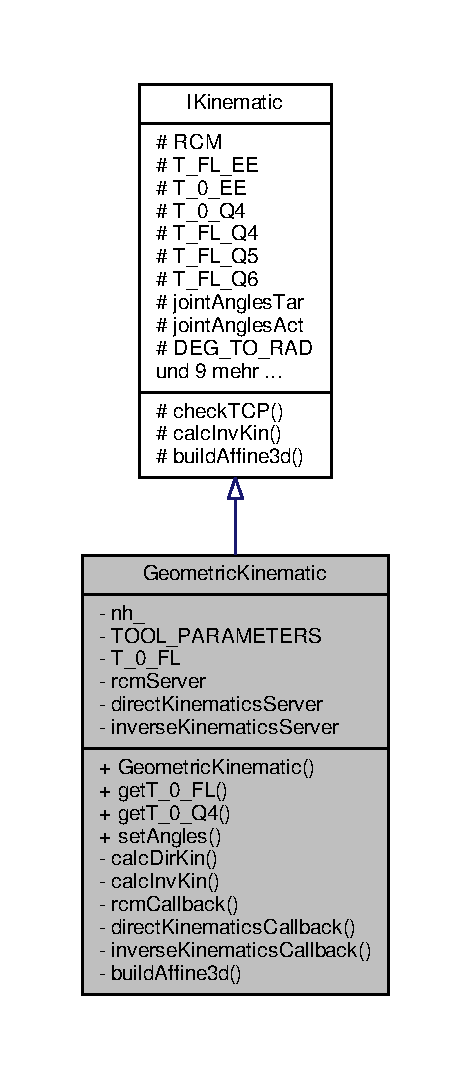
\includegraphics[width=226pt]{classGeometricKinematic__inherit__graph}
\end{center}
\end{figure}


Zusammengehörigkeiten von Geometric\-Kinematic\-:
\nopagebreak
\begin{figure}[H]
\begin{center}
\leavevmode
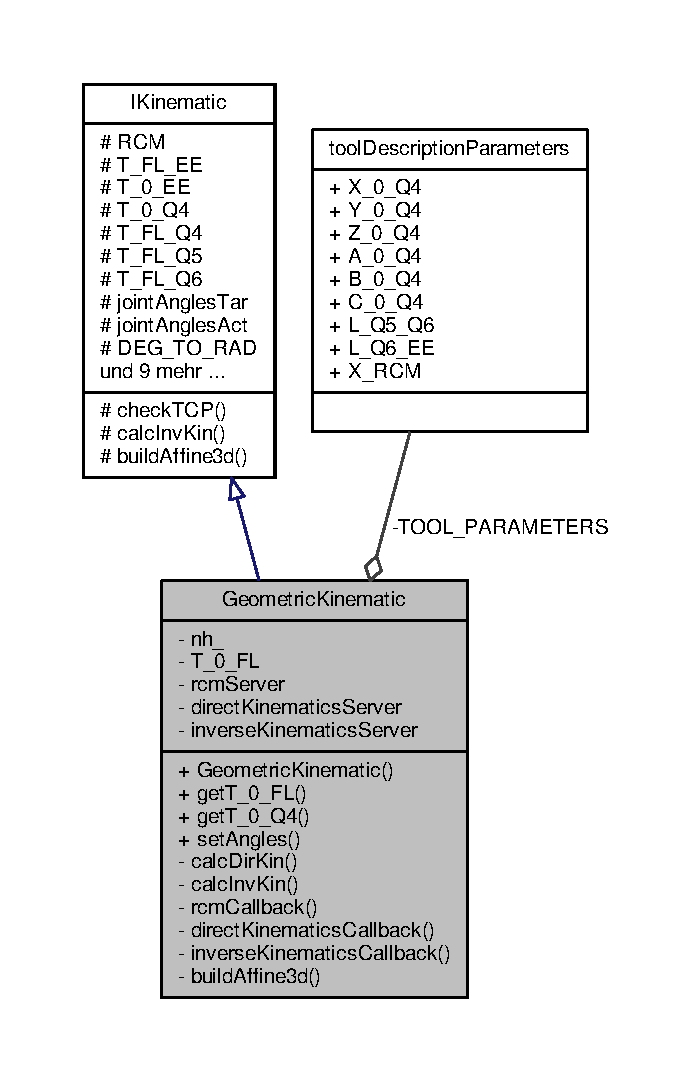
\includegraphics[width=333pt]{classGeometricKinematic__coll__graph}
\end{center}
\end{figure}
\subsection*{Öffentliche Methoden}
\begin{DoxyCompactItemize}
\item 
\hypertarget{classGeometricKinematic_ae9cf7464a179ef36352f1eba1d21999b}{{\bfseries Geometric\-Kinematic} (ros\-::\-Node\-Handle \&)}\label{classGeometricKinematic_ae9cf7464a179ef36352f1eba1d21999b}

\item 
Eigen\-::\-Affine3d \hyperlink{classGeometricKinematic_a2780149e9cc27767a216952be3c4efa1}{get\-T\-\_\-0\-\_\-\-F\-L} ()
\item 
Eigen\-::\-Affine3d \hyperlink{classGeometricKinematic_af17c2b463d3fa83ec26fb4b4d5abb64c}{get\-T\-\_\-0\-\_\-\-Q4} ()
\item 
void \hyperlink{classGeometricKinematic_a985dc4eb67fb7989226d5b8d0ed2f9bf}{set\-Angles} (const Eigen\-::\-Vector\-Xd value)
\end{DoxyCompactItemize}
\subsection*{Private Methoden}
\begin{DoxyCompactItemize}
\item 
Eigen\-::\-Affine3d \hyperlink{classGeometricKinematic_a30ba11c16e6394d094604a8914f97581}{calc\-Dir\-Kin} (Eigen\-::\-Vector\-Xd joint\-Angles)
\begin{DoxyCompactList}\small\item\em Methode zur Berechnung der direkten Kinematik des Werkzeuges. \end{DoxyCompactList}\item 
bool \hyperlink{classGeometricKinematic_a40340db367bf2e3b10830c6ac54be302}{calc\-Inv\-Kin} (Eigen\-::\-Affine3d des\-E\-E\-Position)
\begin{DoxyCompactList}\small\item\em Methode zur Berechnung der inversen Kinematik des Werkzeuges auf Basis geometrischer Bedingungen. \end{DoxyCompactList}\item 
bool \hyperlink{classGeometricKinematic_afd63d5511b3d37eeb2306cb81750e42b}{rcm\-Callback} (masterslave\-::\-Geometric\-Kinematic\-R\-C\-M\-::\-Request \&req, masterslave\-::\-Geometric\-Kinematic\-R\-C\-M\-::\-Response \&resp)
\begin{DoxyCompactList}\small\item\em Callback für den R\-C\-M-\/\-Service, indem der Trokarpunkt berechnet wird. \end{DoxyCompactList}\item 
bool \hyperlink{classGeometricKinematic_ab56c619011ffae14a04162ca09dcc70a}{direct\-Kinematics\-Callback} (masterslave\-::\-Geometric\-Kinematic\-Direct\-Kinematics\-::\-Request \&req, masterslave\-::\-Geometric\-Kinematic\-Direct\-Kinematics\-::\-Response \&resp)
\begin{DoxyCompactList}\small\item\em Callback für den direkten Kinematik-\/\-Service, indem der T\-C\-P berechnet wird. \end{DoxyCompactList}\item 
bool \hyperlink{classGeometricKinematic_ac32c435496ff486133d3aa4094edd2d5}{inverse\-Kinematics\-Callback} (masterslave\-::\-Geometric\-Kinematic\-Inverse\-Kinematics\-::\-Request \&req, masterslave\-::\-Geometric\-Kinematic\-Inverse\-Kinematics\-::\-Response \&resp)
\begin{DoxyCompactList}\small\item\em Callback für den inversen Kinematik-\/\-Service, inder die Flanschlage im Weltkoordinatensystem und die Gelenkwinkel des Werkzeuges berechnet werden. \end{DoxyCompactList}\item 
Eigen\-::\-Affine3d \hyperlink{classGeometricKinematic_a9ed11aaa1279afe9f0f88e52e2f03689}{build\-Affine3d} (const Eigen\-::\-Vector3d \&transl\-X\-Y\-Z, const Eigen\-::\-Vector3d \&axis\-Z\-Y\-X, bool zyx)
\begin{DoxyCompactList}\small\item\em Hilfsfunktion zur Erstellung von Affinen Transformationen aus einem Translationsvekt und den R\-P\-Y-\/\-Winkeln. \end{DoxyCompactList}\end{DoxyCompactItemize}
\subsection*{Private Attribute}
\begin{DoxyCompactItemize}
\item 
\hypertarget{classGeometricKinematic_a3f7a8c38a4444d5fd6daf1da2067799e}{ros\-::\-Node\-Handle {\bfseries nh\-\_\-}}\label{classGeometricKinematic_a3f7a8c38a4444d5fd6daf1da2067799e}

\item 
\hypertarget{classGeometricKinematic_ab3d001b98257b76b051a4c9da08795c0}{const \hyperlink{structtoolDescriptionParameters}{tool\-Description\-Parameters} \hyperlink{classGeometricKinematic_ab3d001b98257b76b051a4c9da08795c0}{T\-O\-O\-L\-\_\-\-P\-A\-R\-A\-M\-E\-T\-E\-R\-S} \{0.\-438, 0.\-0, 0.\-062, 0.\-0, 90.\-0, 0.\-0, 0.\-0088, 0.\-017, 0.\-305\}}\label{classGeometricKinematic_ab3d001b98257b76b051a4c9da08795c0}

\begin{DoxyCompactList}\small\item\em Konstante, die die geometrischen Parameters des laparoskopischen Werkzeuges festlegen (X\-\_\-\-F\-L\-\_\-\-Q4, Y\-\_\-\-F\-L\-\_\-\-Q4, Z\-\_\-\-F\-L\-\_\-\-Q4, A\-\_\-\-F\-L\-\_\-\-Q4, B\-\_\-\-F\-L\-\_\-\-Q4, C\-\_\-\-F\-L\-\_\-\-Q4, X\-\_\-\-Q5\-\_\-\-Q6, X\-\_\-\-Q6\-\_\-\-E\-E, X\-\_\-\-F\-L\-\_\-\-R\-C\-M) \end{DoxyCompactList}\item 
\hypertarget{classGeometricKinematic_a8808661184ee6fe06704b505f27b4dbf}{Eigen\-::\-Affine3d \hyperlink{classGeometricKinematic_a8808661184ee6fe06704b505f27b4dbf}{T\-\_\-0\-\_\-\-F\-L}}\label{classGeometricKinematic_a8808661184ee6fe06704b505f27b4dbf}

\begin{DoxyCompactList}\small\item\em Flanschlage des Roboters im Weltkoordinatensystem. \end{DoxyCompactList}\item 
\hypertarget{classGeometricKinematic_afcf0f9c5c410aaf3fe3aec2d812a42d4}{ros\-::\-Service\-Server \hyperlink{classGeometricKinematic_afcf0f9c5c410aaf3fe3aec2d812a42d4}{rcm\-Server}}\label{classGeometricKinematic_afcf0f9c5c410aaf3fe3aec2d812a42d4}

\begin{DoxyCompactList}\small\item\em Service\-Server für die Bestimmung des Trokarpunktes. \end{DoxyCompactList}\item 
\hypertarget{classGeometricKinematic_a13fabf9990bdab9655b692942c9d4029}{ros\-::\-Service\-Server \hyperlink{classGeometricKinematic_a13fabf9990bdab9655b692942c9d4029}{direct\-Kinematics\-Server}}\label{classGeometricKinematic_a13fabf9990bdab9655b692942c9d4029}

\begin{DoxyCompactList}\small\item\em Service\-Server für die Berechnung des T\-C\-P. \end{DoxyCompactList}\item 
\hypertarget{classGeometricKinematic_aecb5ad028f6a1d165ece2ad904dc9b48}{ros\-::\-Service\-Server \hyperlink{classGeometricKinematic_aecb5ad028f6a1d165ece2ad904dc9b48}{inverse\-Kinematics\-Server}}\label{classGeometricKinematic_aecb5ad028f6a1d165ece2ad904dc9b48}

\begin{DoxyCompactList}\small\item\em Service\-Server für die Berechnung der Gelenkwinkel und der Roboterflanschlage im Weltkoordinatensystem. \end{DoxyCompactList}\end{DoxyCompactItemize}
\subsection*{Weitere Geerbte Elemente}


\subsection{Ausführliche Beschreibung}
Eine Klasse zur Berechnung der Kinematik des Werkzeuges und der Endeffektorlage des L\-B\-R iiwa. 

\begin{DoxyAuthor}{Autor}
Fabian Baier 
\end{DoxyAuthor}
\begin{DoxyDate}{Datum}
20.\-03.\-2016 
\end{DoxyDate}
\begin{DoxySeeAlso}{Siehe auch}
\hyperlink{classIKinematic}{I\-Kinematic} 
\end{DoxySeeAlso}


\subsection{Dokumentation der Elementfunktionen}
\hypertarget{classGeometricKinematic_a9ed11aaa1279afe9f0f88e52e2f03689}{\index{Geometric\-Kinematic@{Geometric\-Kinematic}!build\-Affine3d@{build\-Affine3d}}
\index{build\-Affine3d@{build\-Affine3d}!GeometricKinematic@{Geometric\-Kinematic}}
\subsubsection[{build\-Affine3d}]{\setlength{\rightskip}{0pt plus 5cm}Geometric\-Kinematic\-::build\-Affine3d (
\begin{DoxyParamCaption}
\item[{const Eigen\-::\-Vector3d \&}]{transl\-X\-Y\-Z, }
\item[{const Eigen\-::\-Vector3d \&}]{axis\-Z\-Y\-X, }
\item[{bool}]{zyx}
\end{DoxyParamCaption}
)\hspace{0.3cm}{\ttfamily [private]}}}\label{classGeometricKinematic_a9ed11aaa1279afe9f0f88e52e2f03689}


Hilfsfunktion zur Erstellung von Affinen Transformationen aus einem Translationsvekt und den R\-P\-Y-\/\-Winkeln. 


\begin{DoxyParams}{Parameter}
{\em transl\-X\-Y\-Z} & Translationsvektor \\
\hline
{\em axis\-Z\-Y\-X} & Rotationsvektor \\
\hline
{\em zyx} & Flag zur Festlegung der Rotationsrichtung \\
\hline
\end{DoxyParams}
\begin{DoxyReturn}{Rückgabe}
Affine Transformation 
\end{DoxyReturn}
\hypertarget{classGeometricKinematic_a30ba11c16e6394d094604a8914f97581}{\index{Geometric\-Kinematic@{Geometric\-Kinematic}!calc\-Dir\-Kin@{calc\-Dir\-Kin}}
\index{calc\-Dir\-Kin@{calc\-Dir\-Kin}!GeometricKinematic@{Geometric\-Kinematic}}
\subsubsection[{calc\-Dir\-Kin}]{\setlength{\rightskip}{0pt plus 5cm}Geometric\-Kinematic\-::calc\-Dir\-Kin (
\begin{DoxyParamCaption}
\item[{Eigen\-::\-Vector\-Xd}]{joint\-Angles}
\end{DoxyParamCaption}
)\hspace{0.3cm}{\ttfamily [private]}}}\label{classGeometricKinematic_a30ba11c16e6394d094604a8914f97581}


Methode zur Berechnung der direkten Kinematik des Werkzeuges. 


\begin{DoxyParams}{Parameter}
{\em joint\-Angles} & Gelenkwinkel des Werkzeuges \\
\hline
\end{DoxyParams}
\begin{DoxyReturn}{Rückgabe}
Affine Transformation zwischen Flansch und Endeffektor 
\end{DoxyReturn}
\hypertarget{classGeometricKinematic_a40340db367bf2e3b10830c6ac54be302}{\index{Geometric\-Kinematic@{Geometric\-Kinematic}!calc\-Inv\-Kin@{calc\-Inv\-Kin}}
\index{calc\-Inv\-Kin@{calc\-Inv\-Kin}!GeometricKinematic@{Geometric\-Kinematic}}
\subsubsection[{calc\-Inv\-Kin}]{\setlength{\rightskip}{0pt plus 5cm}Geometric\-Kinematic\-::calc\-Inv\-Kin (
\begin{DoxyParamCaption}
\item[{Eigen\-::\-Affine3d}]{des\-E\-E\-Position}
\end{DoxyParamCaption}
)\hspace{0.3cm}{\ttfamily [private]}, {\ttfamily [virtual]}}}\label{classGeometricKinematic_a40340db367bf2e3b10830c6ac54be302}


Methode zur Berechnung der inversen Kinematik des Werkzeuges auf Basis geometrischer Bedingungen. 


\begin{DoxyParams}{Parameter}
{\em des\-E\-E\-Position} & gewünschte Endeffektorlage im Weltkoordinatensystem \\
\hline
\end{DoxyParams}
\begin{DoxyReturn}{Rückgabe}
Flag, ob der Arbeitsraum eingehalten wurde 
\end{DoxyReturn}


Implementiert \hyperlink{classIKinematic_a6f95d80c4330253643c49a758404e4a7}{I\-Kinematic}.

\hypertarget{classGeometricKinematic_ab56c619011ffae14a04162ca09dcc70a}{\index{Geometric\-Kinematic@{Geometric\-Kinematic}!direct\-Kinematics\-Callback@{direct\-Kinematics\-Callback}}
\index{direct\-Kinematics\-Callback@{direct\-Kinematics\-Callback}!GeometricKinematic@{Geometric\-Kinematic}}
\subsubsection[{direct\-Kinematics\-Callback}]{\setlength{\rightskip}{0pt plus 5cm}Geometric\-Kinematic\-::direct\-Kinematics\-Callback (
\begin{DoxyParamCaption}
\item[{masterslave\-::\-Geometric\-Kinematic\-Direct\-Kinematics\-::\-Request \&}]{req, }
\item[{masterslave\-::\-Geometric\-Kinematic\-Direct\-Kinematics\-::\-Response \&}]{resp}
\end{DoxyParamCaption}
)\hspace{0.3cm}{\ttfamily [private]}}}\label{classGeometricKinematic_ab56c619011ffae14a04162ca09dcc70a}


Callback für den direkten Kinematik-\/\-Service, indem der T\-C\-P berechnet wird. 


\begin{DoxyParams}{Parameter}
{\em req} & L\-B\-R-\/\-Flanschlage und Gelenkwinkel des Werkzeuges \\
\hline
{\em resp} & Aktueller T\-C\-P im Weltkoordinatensystem \\
\hline
\end{DoxyParams}
\begin{DoxyReturn}{Rückgabe}
Flag, ob der Serviceaufruf erfolgreich war 
\end{DoxyReturn}
\begin{DoxySeeAlso}{Siehe auch}
Geometric\-Kinematic\-Direct\-Kinematic.\-srv 
\end{DoxySeeAlso}
\hypertarget{classGeometricKinematic_a2780149e9cc27767a216952be3c4efa1}{\index{Geometric\-Kinematic@{Geometric\-Kinematic}!get\-T\-\_\-0\-\_\-\-F\-L@{get\-T\-\_\-0\-\_\-\-F\-L}}
\index{get\-T\-\_\-0\-\_\-\-F\-L@{get\-T\-\_\-0\-\_\-\-F\-L}!GeometricKinematic@{Geometric\-Kinematic}}
\subsubsection[{get\-T\-\_\-0\-\_\-\-F\-L}]{\setlength{\rightskip}{0pt plus 5cm}Geometric\-Kinematic\-::get\-T\-\_\-0\-\_\-\-F\-L (
\begin{DoxyParamCaption}
{}
\end{DoxyParamCaption}
)\hspace{0.3cm}{\ttfamily [inline]}}}\label{classGeometricKinematic_a2780149e9cc27767a216952be3c4efa1}
\begin{DoxyRefDesc}{Noch zu erledigen}
\item[\hyperlink{todo__todo000008}{Noch zu erledigen}]check ob noch benötigt \begin{DoxyReturn}{Rückgabe}

\end{DoxyReturn}
\end{DoxyRefDesc}
\hypertarget{classGeometricKinematic_af17c2b463d3fa83ec26fb4b4d5abb64c}{\index{Geometric\-Kinematic@{Geometric\-Kinematic}!get\-T\-\_\-0\-\_\-\-Q4@{get\-T\-\_\-0\-\_\-\-Q4}}
\index{get\-T\-\_\-0\-\_\-\-Q4@{get\-T\-\_\-0\-\_\-\-Q4}!GeometricKinematic@{Geometric\-Kinematic}}
\subsubsection[{get\-T\-\_\-0\-\_\-\-Q4}]{\setlength{\rightskip}{0pt plus 5cm}Geometric\-Kinematic\-::get\-T\-\_\-0\-\_\-\-Q4 (
\begin{DoxyParamCaption}
{}
\end{DoxyParamCaption}
)\hspace{0.3cm}{\ttfamily [inline]}}}\label{classGeometricKinematic_af17c2b463d3fa83ec26fb4b4d5abb64c}
\begin{DoxyRefDesc}{Noch zu erledigen}
\item[\hyperlink{todo__todo000009}{Noch zu erledigen}]check ob noch benötigt \begin{DoxyReturn}{Rückgabe}

\end{DoxyReturn}
\end{DoxyRefDesc}
\hypertarget{classGeometricKinematic_ac32c435496ff486133d3aa4094edd2d5}{\index{Geometric\-Kinematic@{Geometric\-Kinematic}!inverse\-Kinematics\-Callback@{inverse\-Kinematics\-Callback}}
\index{inverse\-Kinematics\-Callback@{inverse\-Kinematics\-Callback}!GeometricKinematic@{Geometric\-Kinematic}}
\subsubsection[{inverse\-Kinematics\-Callback}]{\setlength{\rightskip}{0pt plus 5cm}Geometric\-Kinematic\-::inverse\-Kinematics\-Callback (
\begin{DoxyParamCaption}
\item[{masterslave\-::\-Geometric\-Kinematic\-Inverse\-Kinematics\-::\-Request \&}]{req, }
\item[{masterslave\-::\-Geometric\-Kinematic\-Inverse\-Kinematics\-::\-Response \&}]{resp}
\end{DoxyParamCaption}
)\hspace{0.3cm}{\ttfamily [private]}}}\label{classGeometricKinematic_ac32c435496ff486133d3aa4094edd2d5}


Callback für den inversen Kinematik-\/\-Service, inder die Flanschlage im Weltkoordinatensystem und die Gelenkwinkel des Werkzeuges berechnet werden. 


\begin{DoxyParams}{Parameter}
{\em req} & Gewünschter T\-C\-P im Weltkoordinatensystem \\
\hline
{\em resp} & L\-B\-R-\/\-Flanschlage im Weltkoordinatensystem und Gelenkwinkel des Werkzeuges \\
\hline
\end{DoxyParams}
\begin{DoxyReturn}{Rückgabe}
Flag, ob der Serviceaufruf erfolgreich war 
\end{DoxyReturn}
\begin{DoxySeeAlso}{Siehe auch}
Geometric\-Kinematic\-Inverse\-Kinematic.\-srv 
\end{DoxySeeAlso}
\hypertarget{classGeometricKinematic_afd63d5511b3d37eeb2306cb81750e42b}{\index{Geometric\-Kinematic@{Geometric\-Kinematic}!rcm\-Callback@{rcm\-Callback}}
\index{rcm\-Callback@{rcm\-Callback}!GeometricKinematic@{Geometric\-Kinematic}}
\subsubsection[{rcm\-Callback}]{\setlength{\rightskip}{0pt plus 5cm}Geometric\-Kinematic\-::rcm\-Callback (
\begin{DoxyParamCaption}
\item[{masterslave\-::\-Geometric\-Kinematic\-R\-C\-M\-::\-Request \&}]{req, }
\item[{masterslave\-::\-Geometric\-Kinematic\-R\-C\-M\-::\-Response \&}]{resp}
\end{DoxyParamCaption}
)\hspace{0.3cm}{\ttfamily [private]}}}\label{classGeometricKinematic_afd63d5511b3d37eeb2306cb81750e42b}


Callback für den R\-C\-M-\/\-Service, indem der Trokarpunkt berechnet wird. 


\begin{DoxyParams}{Parameter}
{\em req} & L\-B\-R-\/\-Startposition \\
\hline
{\em resp} & Trokarpunkt im Weltkoordinatensystem \\
\hline
\end{DoxyParams}
\begin{DoxyReturn}{Rückgabe}
Flag, ob der Serviceaufruf erfolgreich war 
\end{DoxyReturn}
\begin{DoxySeeAlso}{Siehe auch}
Geometric\-Kinematic\-R\-C\-M.\-srv 
\end{DoxySeeAlso}
\hypertarget{classGeometricKinematic_a985dc4eb67fb7989226d5b8d0ed2f9bf}{\index{Geometric\-Kinematic@{Geometric\-Kinematic}!set\-Angles@{set\-Angles}}
\index{set\-Angles@{set\-Angles}!GeometricKinematic@{Geometric\-Kinematic}}
\subsubsection[{set\-Angles}]{\setlength{\rightskip}{0pt plus 5cm}Geometric\-Kinematic\-::set\-Angles (
\begin{DoxyParamCaption}
\item[{const Eigen\-::\-Vector\-Xd}]{value}
\end{DoxyParamCaption}
)}}\label{classGeometricKinematic_a985dc4eb67fb7989226d5b8d0ed2f9bf}

\begin{DoxyParams}{Parameter}
{\em value} & \\
\hline
\end{DoxyParams}
\begin{DoxyRefDesc}{Noch zu erledigen}
\item[\hyperlink{todo__todo000010}{Noch zu erledigen}]check ob noch benötigt, da jetzt über Services kommuniziert wird \end{DoxyRefDesc}


Die Dokumentation für diese Klasse wurde erzeugt aufgrund der Datei\-:\begin{DoxyCompactItemize}
\item 
include/masterslave/kinematic/\hyperlink{GeometricKinematic_8h}{Geometric\-Kinematic.\-h}\end{DoxyCompactItemize}

\hypertarget{classGeometricKinematicCommander}{\section{Geometric\-Kinematic\-Commander Klassenreferenz}
\label{classGeometricKinematicCommander}\index{Geometric\-Kinematic\-Commander@{Geometric\-Kinematic\-Commander}}
}


Klasse, die sich um die R\-O\-S-\/\-Kommunikation für die geometrisch bestimmte Kinematik kümmert.  




{\ttfamily \#include $<$Geometric\-Kinematic\-Commander.\-h$>$}



Klassendiagramm für Geometric\-Kinematic\-Commander\-:
\nopagebreak
\begin{figure}[H]
\begin{center}
\leavevmode
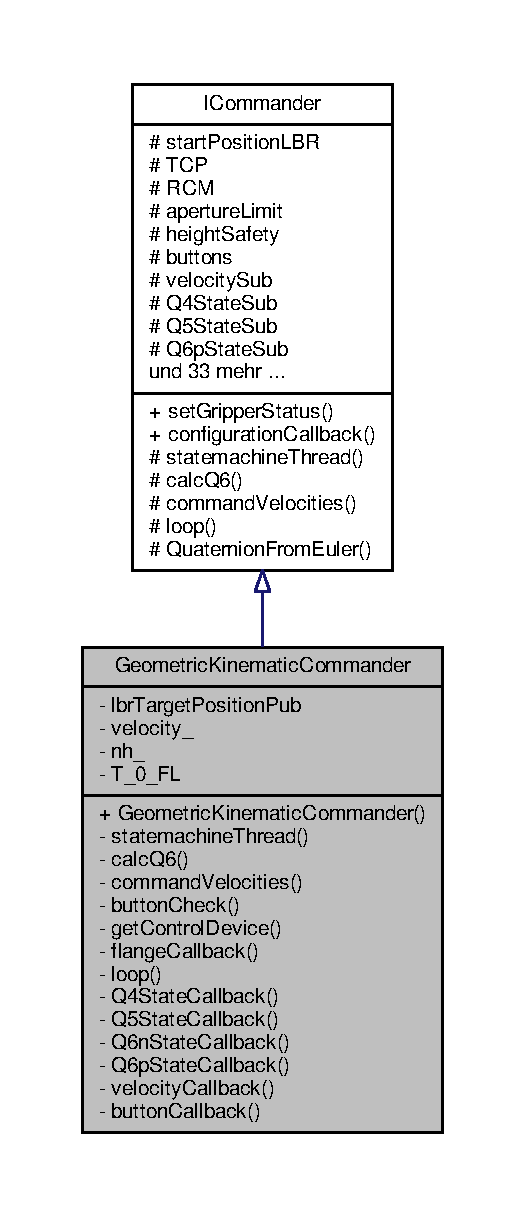
\includegraphics[height=550pt]{classGeometricKinematicCommander__inherit__graph}
\end{center}
\end{figure}


Zusammengehörigkeiten von Geometric\-Kinematic\-Commander\-:
\nopagebreak
\begin{figure}[H]
\begin{center}
\leavevmode
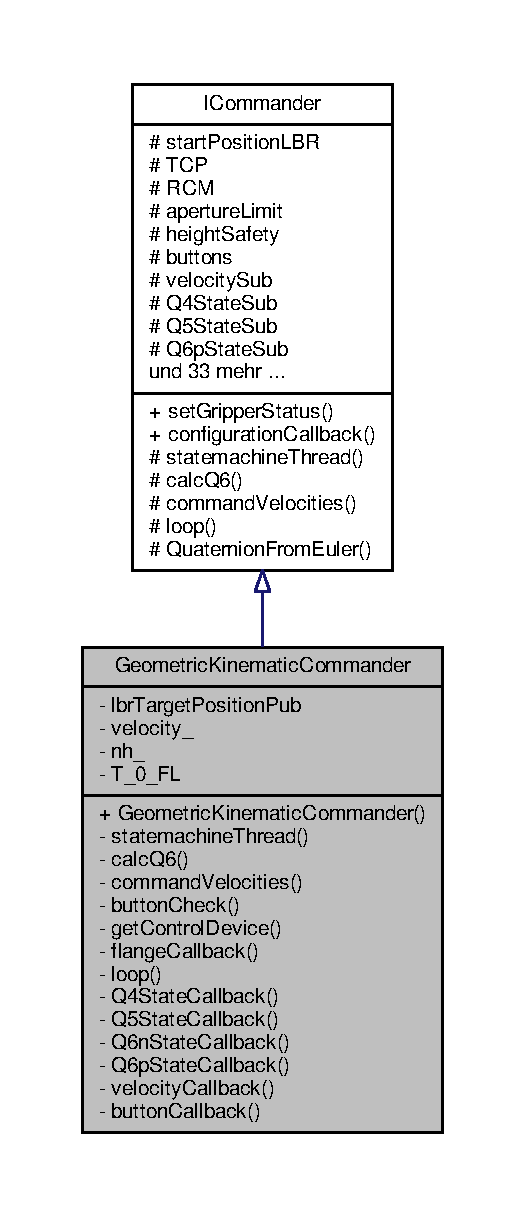
\includegraphics[height=550pt]{classGeometricKinematicCommander__coll__graph}
\end{center}
\end{figure}
\subsection*{Öffentliche Methoden}
\begin{DoxyCompactItemize}
\item 
\hypertarget{classGeometricKinematicCommander_a7bb3cf43a3e4f09f71433f11af17dfcc}{{\bfseries Geometric\-Kinematic\-Commander} (ros\-::\-Node\-Handle \&nh, ros\-::\-Node\-Handle \&dr\-N\-H)}\label{classGeometricKinematicCommander_a7bb3cf43a3e4f09f71433f11af17dfcc}

\end{DoxyCompactItemize}
\subsection*{Private Methoden}
\begin{DoxyCompactItemize}
\item 
void \hyperlink{classGeometricKinematicCommander_a85c8118bd74639548f6791880aeb8f81}{statemachine\-Thread} (const ros\-::\-Timer\-Event \&)
\begin{DoxyCompactList}\small\item\em Thread der alle 20ms aufgerufen wird und den Status an R\-O\-S\-Open\-I\-G\-T\-L\-Bridge schickt. \end{DoxyCompactList}\item 
void \hyperlink{classGeometricKinematicCommander_a8f2f1e6428ae88ccdd630d59eff6d5af}{calc\-Q6} ()
\begin{DoxyCompactList}\small\item\em Berechnet aus dem Gelenkwinkel Q6 die Gelenkwinkel Q6n und Q6p des Zangengreifers. \end{DoxyCompactList}\item 
void \hyperlink{classGeometricKinematicCommander_a79cc755ef52804b1cbd1e71dd2f77339}{command\-Velocities} ()
\begin{DoxyCompactList}\small\item\em Schickt die Gelenkwinkelgeschwindigkeiten an die Nodes der Antriebe des Werkzeuges. \end{DoxyCompactList}\item 
void \hyperlink{classGeometricKinematicCommander_a54f853173048f2d5b55c00d711e3542a}{button\-Check} ()
\begin{DoxyCompactList}\small\item\em Die Methode holt die Knopfkonfiguration vom Parameterserver. \end{DoxyCompactList}\item 
void \hyperlink{classGeometricKinematicCommander_a91fbbc67883244f37fff899029855140}{get\-Control\-Device} ()
\begin{DoxyCompactList}\small\item\em Die Methode findet den Typ des Eingabegerätes auf dem Parameterserver. \end{DoxyCompactList}\item 
\hypertarget{classGeometricKinematicCommander_a61edc35487744095113c99b29b7c57bd}{void \hyperlink{classGeometricKinematicCommander_a61edc35487744095113c99b29b7c57bd}{flange\-Callback} (const geometry\-\_\-msgs\-::\-Pose\-Stamped\-Const\-Ptr \&)}\label{classGeometricKinematicCommander_a61edc35487744095113c99b29b7c57bd}

\begin{DoxyCompactList}\small\item\em Methode zum Empfang der aktuellen Roboterflanschlage. \end{DoxyCompactList}\item 
void \hyperlink{classGeometricKinematicCommander_aa813582c3cf973c6704dc24077150b3b}{loop} ()
\item 
\hypertarget{classGeometricKinematicCommander_afe8ae9fce613511a87435a920eaa6299}{void {\bfseries Q4\-State\-Callback} (const sensor\-\_\-msgs\-::\-Joint\-State\-Const\-Ptr \&\hyperlink{classICommander_a72cb524deeb95b224db0242efc4728d4}{state})}\label{classGeometricKinematicCommander_afe8ae9fce613511a87435a920eaa6299}

\item 
\hypertarget{classGeometricKinematicCommander_aad8e587222c5aef18ebb28e5df2afbbc}{void {\bfseries Q5\-State\-Callback} (const sensor\-\_\-msgs\-::\-Joint\-State\-Const\-Ptr \&\hyperlink{classICommander_a72cb524deeb95b224db0242efc4728d4}{state})}\label{classGeometricKinematicCommander_aad8e587222c5aef18ebb28e5df2afbbc}

\item 
\hypertarget{classGeometricKinematicCommander_a08ace2af8ea41575b97d4e64425fdd5c}{void {\bfseries Q6n\-State\-Callback} (const sensor\-\_\-msgs\-::\-Joint\-State\-Const\-Ptr \&\hyperlink{classICommander_a72cb524deeb95b224db0242efc4728d4}{state})}\label{classGeometricKinematicCommander_a08ace2af8ea41575b97d4e64425fdd5c}

\item 
\hypertarget{classGeometricKinematicCommander_ad227d224cca51469aed89e3f63a2224b}{void {\bfseries Q6p\-State\-Callback} (const sensor\-\_\-msgs\-::\-Joint\-State\-Const\-Ptr \&\hyperlink{classICommander_a72cb524deeb95b224db0242efc4728d4}{state})}\label{classGeometricKinematicCommander_ad227d224cca51469aed89e3f63a2224b}

\item 
\hypertarget{classGeometricKinematicCommander_a86060fb1189ba2d304bcab2f058609b1}{void {\bfseries velocity\-Callback} (const geometry\-\_\-msgs\-::\-Twist\-Stamped\-Const\-Ptr \&)}\label{classGeometricKinematicCommander_a86060fb1189ba2d304bcab2f058609b1}

\item 
\hypertarget{classGeometricKinematicCommander_a780e85603f9b7201784cfb09706734ae}{void {\bfseries button\-Callback} (const masterslave\-::\-Button\-Const\-Ptr \&)}\label{classGeometricKinematicCommander_a780e85603f9b7201784cfb09706734ae}

\end{DoxyCompactItemize}
\subsection*{Private Attribute}
\begin{DoxyCompactItemize}
\item 
\hypertarget{classGeometricKinematicCommander_ab2d3302d1b9cdad6bc363403811b6e5e}{ros\-::\-Publisher \hyperlink{classGeometricKinematicCommander_ab2d3302d1b9cdad6bc363403811b6e5e}{lbr\-Target\-Position\-Pub}}\label{classGeometricKinematicCommander_ab2d3302d1b9cdad6bc363403811b6e5e}

\begin{DoxyCompactList}\small\item\em Sender der L\-B\-R-\/\-Flanschlage in R\-O\-S. \end{DoxyCompactList}\item 
geometry\-\_\-msgs\-::\-Twist\-Stamped \hyperlink{classGeometricKinematicCommander_afbfee50f578ff4098026413f41b916a3}{velocity\-\_\-}
\item 
\hypertarget{classGeometricKinematicCommander_a9aa4841981737548fa4dc94d7ddec84a}{ros\-::\-Node\-Handle {\bfseries nh\-\_\-}}\label{classGeometricKinematicCommander_a9aa4841981737548fa4dc94d7ddec84a}

\item 
\hypertarget{classGeometricKinematicCommander_ae58f3ee72e4ff68fe5d4e720e42cddbc}{Eigen\-::\-Affine3d \hyperlink{classGeometricKinematicCommander_ae58f3ee72e4ff68fe5d4e720e42cddbc}{T\-\_\-0\-\_\-\-F\-L}}\label{classGeometricKinematicCommander_ae58f3ee72e4ff68fe5d4e720e42cddbc}

\begin{DoxyCompactList}\small\item\em Roboterflanschlage des L\-B\-R iiwa. \end{DoxyCompactList}\end{DoxyCompactItemize}
\subsection*{Weitere Geerbte Elemente}


\subsection{Ausführliche Beschreibung}
Klasse, die sich um die R\-O\-S-\/\-Kommunikation für die geometrisch bestimmte Kinematik kümmert. 

\begin{DoxyAuthor}{Autor}
Fabian Baier 
\end{DoxyAuthor}
\begin{DoxyDate}{Datum}
19.\-03.\-2016 
\end{DoxyDate}
\begin{DoxySeeAlso}{Siehe auch}
\hyperlink{classICommander}{I\-Commander} 
\end{DoxySeeAlso}


\subsection{Dokumentation der Elementfunktionen}
\hypertarget{classGeometricKinematicCommander_a54f853173048f2d5b55c00d711e3542a}{\index{Geometric\-Kinematic\-Commander@{Geometric\-Kinematic\-Commander}!button\-Check@{button\-Check}}
\index{button\-Check@{button\-Check}!GeometricKinematicCommander@{Geometric\-Kinematic\-Commander}}
\subsubsection[{button\-Check}]{\setlength{\rightskip}{0pt plus 5cm}Geometric\-Kinematic\-Commander\-::button\-Check (
\begin{DoxyParamCaption}
{}
\end{DoxyParamCaption}
)\hspace{0.3cm}{\ttfamily [private]}}}\label{classGeometricKinematicCommander_a54f853173048f2d5b55c00d711e3542a}


Die Methode holt die Knopfkonfiguration vom Parameterserver. 

\begin{DoxySeeAlso}{Siehe auch}
\hyperlink{classControlDevice}{Control\-Device} 
\end{DoxySeeAlso}
\hypertarget{classGeometricKinematicCommander_a8f2f1e6428ae88ccdd630d59eff6d5af}{\index{Geometric\-Kinematic\-Commander@{Geometric\-Kinematic\-Commander}!calc\-Q6@{calc\-Q6}}
\index{calc\-Q6@{calc\-Q6}!GeometricKinematicCommander@{Geometric\-Kinematic\-Commander}}
\subsubsection[{calc\-Q6}]{\setlength{\rightskip}{0pt plus 5cm}Geometric\-Kinematic\-Commander\-::calc\-Q6 (
\begin{DoxyParamCaption}
{}
\end{DoxyParamCaption}
)\hspace{0.3cm}{\ttfamily [private]}, {\ttfamily [virtual]}}}\label{classGeometricKinematicCommander_a8f2f1e6428ae88ccdd630d59eff6d5af}


Berechnet aus dem Gelenkwinkel Q6 die Gelenkwinkel Q6n und Q6p des Zangengreifers. 

\begin{DoxySeeAlso}{Siehe auch}
\hyperlink{classICommander}{I\-Commander} 
\end{DoxySeeAlso}


Implementiert \hyperlink{classICommander_a1967688a309974862c4a81b5fe04c3eb}{I\-Commander}.

\hypertarget{classGeometricKinematicCommander_a79cc755ef52804b1cbd1e71dd2f77339}{\index{Geometric\-Kinematic\-Commander@{Geometric\-Kinematic\-Commander}!command\-Velocities@{command\-Velocities}}
\index{command\-Velocities@{command\-Velocities}!GeometricKinematicCommander@{Geometric\-Kinematic\-Commander}}
\subsubsection[{command\-Velocities}]{\setlength{\rightskip}{0pt plus 5cm}Geometric\-Kinematic\-Commander\-::command\-Velocities (
\begin{DoxyParamCaption}
{}
\end{DoxyParamCaption}
)\hspace{0.3cm}{\ttfamily [private]}, {\ttfamily [virtual]}}}\label{classGeometricKinematicCommander_a79cc755ef52804b1cbd1e71dd2f77339}


Schickt die Gelenkwinkelgeschwindigkeiten an die Nodes der Antriebe des Werkzeuges. 

\begin{DoxySeeAlso}{Siehe auch}
\hyperlink{classICommander}{I\-Commander} 
\end{DoxySeeAlso}


Implementiert \hyperlink{classICommander_a43c10dd80f4815afd4058226450c7af3}{I\-Commander}.

\hypertarget{classGeometricKinematicCommander_a91fbbc67883244f37fff899029855140}{\index{Geometric\-Kinematic\-Commander@{Geometric\-Kinematic\-Commander}!get\-Control\-Device@{get\-Control\-Device}}
\index{get\-Control\-Device@{get\-Control\-Device}!GeometricKinematicCommander@{Geometric\-Kinematic\-Commander}}
\subsubsection[{get\-Control\-Device}]{\setlength{\rightskip}{0pt plus 5cm}Geometric\-Kinematic\-Commander\-::get\-Control\-Device (
\begin{DoxyParamCaption}
{}
\end{DoxyParamCaption}
)\hspace{0.3cm}{\ttfamily [private]}}}\label{classGeometricKinematicCommander_a91fbbc67883244f37fff899029855140}


Die Methode findet den Typ des Eingabegerätes auf dem Parameterserver. 

\begin{DoxySeeAlso}{Siehe auch}
\hyperlink{classControlDevice}{Control\-Device} 
\end{DoxySeeAlso}
\hypertarget{classGeometricKinematicCommander_aa813582c3cf973c6704dc24077150b3b}{\index{Geometric\-Kinematic\-Commander@{Geometric\-Kinematic\-Commander}!loop@{loop}}
\index{loop@{loop}!GeometricKinematicCommander@{Geometric\-Kinematic\-Commander}}
\subsubsection[{loop}]{\setlength{\rightskip}{0pt plus 5cm}Geometric\-Kinematic\-Commander\-::loop (
\begin{DoxyParamCaption}
{}
\end{DoxyParamCaption}
)\hspace{0.3cm}{\ttfamily [private]}, {\ttfamily [virtual]}}}\label{classGeometricKinematicCommander_aa813582c3cf973c6704dc24077150b3b}
\begin{DoxySeeAlso}{Siehe auch}
\hyperlink{classICommander}{I\-Commander} 
\end{DoxySeeAlso}


Implementiert \hyperlink{classICommander_aa5f882f46d3629fa754162a9ee11984c}{I\-Commander}.

\hypertarget{classGeometricKinematicCommander_a85c8118bd74639548f6791880aeb8f81}{\index{Geometric\-Kinematic\-Commander@{Geometric\-Kinematic\-Commander}!statemachine\-Thread@{statemachine\-Thread}}
\index{statemachine\-Thread@{statemachine\-Thread}!GeometricKinematicCommander@{Geometric\-Kinematic\-Commander}}
\subsubsection[{statemachine\-Thread}]{\setlength{\rightskip}{0pt plus 5cm}Geometric\-Kinematic\-Commander\-::statemachine\-Thread (
\begin{DoxyParamCaption}
\item[{const ros\-::\-Timer\-Event \&}]{}
\end{DoxyParamCaption}
)\hspace{0.3cm}{\ttfamily [private]}, {\ttfamily [virtual]}}}\label{classGeometricKinematicCommander_a85c8118bd74639548f6791880aeb8f81}


Thread der alle 20ms aufgerufen wird und den Status an R\-O\-S\-Open\-I\-G\-T\-L\-Bridge schickt. 

\begin{DoxySeeAlso}{Siehe auch}
\hyperlink{classICommander}{I\-Commander} 
\end{DoxySeeAlso}


Implementiert \hyperlink{classICommander_abcacd07f49f646d08e1722a1df08b8ce}{I\-Commander}.



\subsection{Dokumentation der Datenelemente}
\hypertarget{classGeometricKinematicCommander_afbfee50f578ff4098026413f41b916a3}{\index{Geometric\-Kinematic\-Commander@{Geometric\-Kinematic\-Commander}!velocity\-\_\-@{velocity\-\_\-}}
\index{velocity\-\_\-@{velocity\-\_\-}!GeometricKinematicCommander@{Geometric\-Kinematic\-Commander}}
\subsubsection[{velocity\-\_\-}]{\setlength{\rightskip}{0pt plus 5cm}Geometric\-Kinematic\-Commander\-::velocity\-\_\-\hspace{0.3cm}{\ttfamily [private]}}}\label{classGeometricKinematicCommander_afbfee50f578ff4098026413f41b916a3}
\begin{DoxyRefDesc}{Noch zu erledigen}
\item[\hyperlink{todo__todo000001}{Noch zu erledigen}]check ob noch benötigt \end{DoxyRefDesc}


Die Dokumentation für diese Klasse wurde erzeugt aufgrund der Datei\-:\begin{DoxyCompactItemize}
\item 
include/masterslave/commander/\hyperlink{GeometricKinematicCommander_8h}{Geometric\-Kinematic\-Commander.\-h}\end{DoxyCompactItemize}

\hypertarget{classICommander}{\section{I\-Commander Klassenreferenz}
\label{classICommander}\index{I\-Commander@{I\-Commander}}
}


Abstrakte Basisklasse zur Ansteuerung der beiden Kinematikmodelle über R\-O\-S.  




{\ttfamily \#include $<$I\-Commander.\-h$>$}



Klassendiagramm für I\-Commander\-:
\nopagebreak
\begin{figure}[H]
\begin{center}
\leavevmode
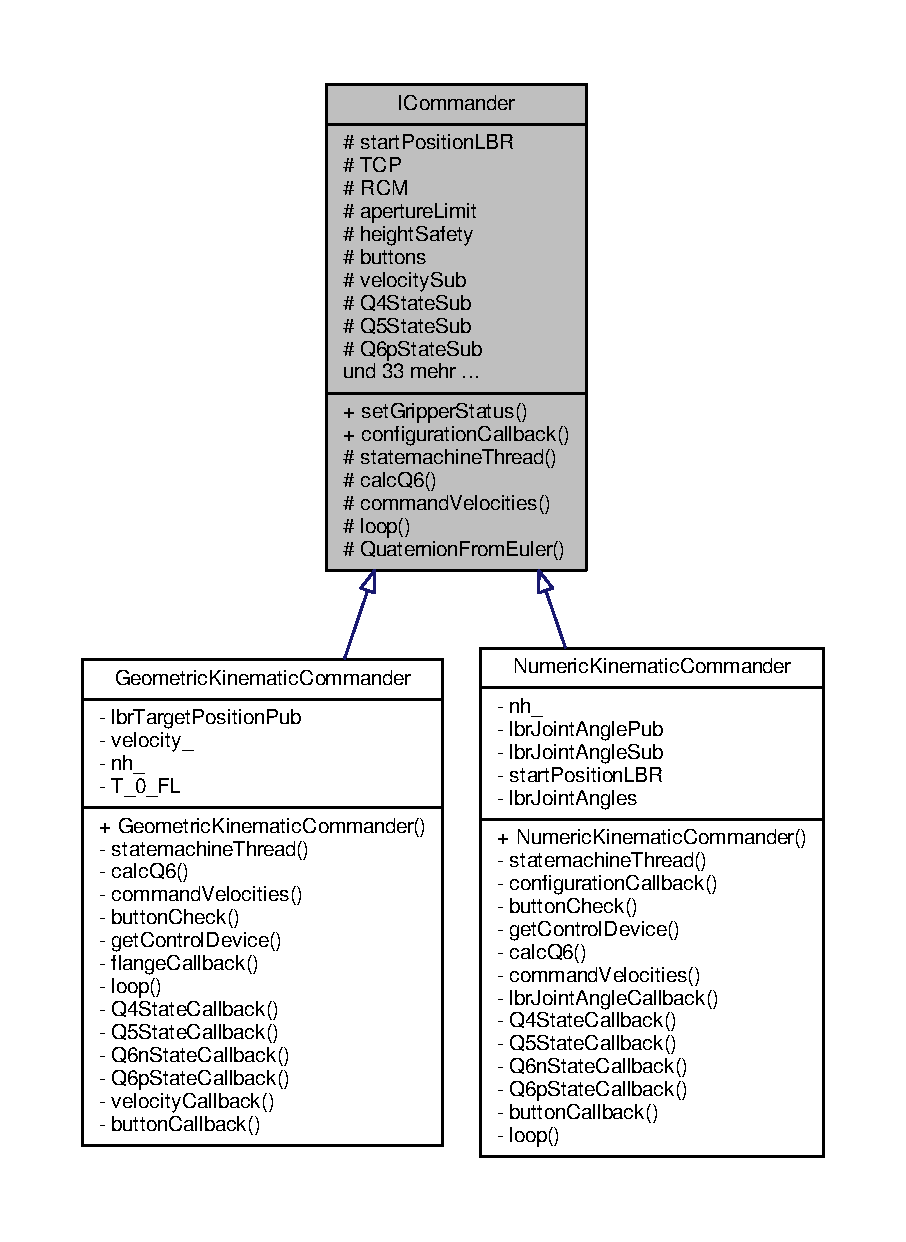
\includegraphics[width=350pt]{classICommander__inherit__graph}
\end{center}
\end{figure}


Zusammengehörigkeiten von I\-Commander\-:
\nopagebreak
\begin{figure}[H]
\begin{center}
\leavevmode
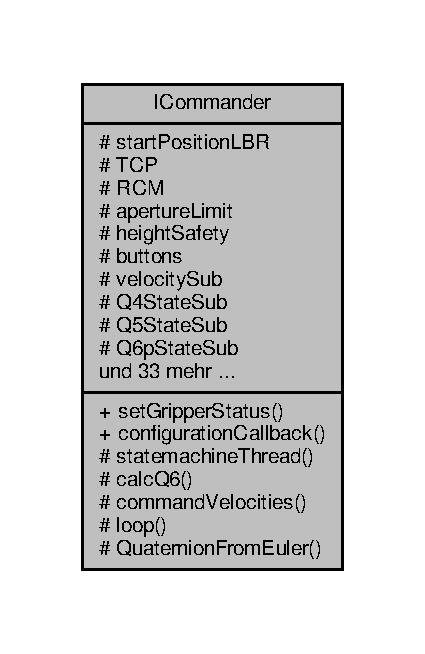
\includegraphics[width=204pt]{classICommander__coll__graph}
\end{center}
\end{figure}
\subsection*{Öffentliche Methoden}
\begin{DoxyCompactItemize}
\item 
void \hyperlink{classICommander_a8a9f1636cbe5526d490266be84e6a57f}{set\-Gripper\-Status} (bool open, bool close)
\item 
void \hyperlink{classICommander_a9c55ba4a6c61efe9dc33ed76fd180a4e}{configuration\-Callback} (masterslave\-::\-Master\-Slave\-Config \&config, uint32\-\_\-t level)
\begin{DoxyCompactList}\small\item\em dynamic reconfigure Callbackmethode \end{DoxyCompactList}\end{DoxyCompactItemize}
\subsection*{Geschützte Methoden}
\begin{DoxyCompactItemize}
\item 
\hypertarget{classICommander_abcacd07f49f646d08e1722a1df08b8ce}{virtual void \hyperlink{classICommander_abcacd07f49f646d08e1722a1df08b8ce}{statemachine\-Thread} (const ros\-::\-Timer\-Event \&)=0}\label{classICommander_abcacd07f49f646d08e1722a1df08b8ce}

\begin{DoxyCompactList}\small\item\em abstrakte Methode um den Zustand des Open\-I\-G\-T\-Link\-Interfaces wechseln \end{DoxyCompactList}\item 
\hypertarget{classICommander_a1967688a309974862c4a81b5fe04c3eb}{virtual void \hyperlink{classICommander_a1967688a309974862c4a81b5fe04c3eb}{calc\-Q6} ()=0}\label{classICommander_a1967688a309974862c4a81b5fe04c3eb}

\begin{DoxyCompactList}\small\item\em Die abstrakte Methode berechnet aus dem Gelenkwinkel Q6 die Gelenkwinkel Q6n und Q6p des Zangengreifers. \end{DoxyCompactList}\item 
\hypertarget{classICommander_a43c10dd80f4815afd4058226450c7af3}{virtual void \hyperlink{classICommander_a43c10dd80f4815afd4058226450c7af3}{command\-Velocities} ()=0}\label{classICommander_a43c10dd80f4815afd4058226450c7af3}

\begin{DoxyCompactList}\small\item\em Die abstrakte Methode übernimmt die Kommandierung der Gelenkwinkel. \end{DoxyCompactList}\item 
\hypertarget{classICommander_aa5f882f46d3629fa754162a9ee11984c}{virtual void \hyperlink{classICommander_aa5f882f46d3629fa754162a9ee11984c}{loop} ()=0}\label{classICommander_aa5f882f46d3629fa754162a9ee11984c}

\begin{DoxyCompactList}\small\item\em Die abstrakte Methode übernimmt je nach Implementierung die Kommunikation mit dem Roboter bzw. der Simulation und der Kinematikklasse über R\-O\-S-\/\-Servies. \end{DoxyCompactList}\item 
Eigen\-::\-Quaternion$<$ double $>$ \hyperlink{classICommander_a3f9e89737d7d924553d2ed6704eb8af7}{Quaternion\-From\-Euler} (const Eigen\-::\-Vector3d \&euler\-X\-Y\-Z, bool Z\-Y\-X)
\begin{DoxyCompactList}\small\item\em Hilfsmethode um ein Quaternion aus Eulerwinkel zu erstellen. \end{DoxyCompactList}\end{DoxyCompactItemize}
\subsection*{Geschützte Attribute}
\begin{DoxyCompactItemize}
\item 
\hypertarget{classICommander_af6a774cc1d571b4858ebae680d1f0939}{Eigen\-::\-Affine3d \hyperlink{classICommander_af6a774cc1d571b4858ebae680d1f0939}{start\-Position\-L\-B\-R}}\label{classICommander_af6a774cc1d571b4858ebae680d1f0939}

\begin{DoxyCompactList}\small\item\em kartesische Startposition des Endeffektors des L\-B\-R \end{DoxyCompactList}\item 
\hypertarget{classICommander_a8762a3ea77233f9700166908ad4d1987}{Eigen\-::\-Affine3d \hyperlink{classICommander_a8762a3ea77233f9700166908ad4d1987}{T\-C\-P}}\label{classICommander_a8762a3ea77233f9700166908ad4d1987}

\begin{DoxyCompactList}\small\item\em kartesische Startposition des T\-C\-P des Werkzeuges \end{DoxyCompactList}\item 
\hypertarget{classICommander_aec4eecfaa992cfb2ede1f1d339548326}{Eigen\-::\-Affine3d \hyperlink{classICommander_aec4eecfaa992cfb2ede1f1d339548326}{R\-C\-M}}\label{classICommander_aec4eecfaa992cfb2ede1f1d339548326}

\begin{DoxyCompactList}\small\item\em Trokarpunkt. \end{DoxyCompactList}\item 
double \hyperlink{classICommander_a01ec4010dc037bfb600cee7f0be9311c}{aperture\-Limit}
\item 
double \hyperlink{classICommander_a166295c90210dae6c74e96d749c8ea1a}{height\-Safety}
\item 
std\-::vector$<$ std\-::string $>$ \hyperlink{classICommander_a038f78434eb525d73414c84624d3c3e4}{buttons}
\begin{DoxyCompactList}\small\item\em Vektor, der die Knopfkonfiguration enthält. \end{DoxyCompactList}\item 
ros\-::\-Subscriber \hyperlink{classICommander_a77d12525f98994352e2f2a450e04305b}{velocity\-Sub}
\item 
\hypertarget{classICommander_aaf7b291fe6f704d0a05ca9c51c00eee5}{ros\-::\-Subscriber \hyperlink{classICommander_aaf7b291fe6f704d0a05ca9c51c00eee5}{Q4\-State\-Sub}}\label{classICommander_aaf7b291fe6f704d0a05ca9c51c00eee5}

\begin{DoxyCompactList}\small\item\em Empfänger in R\-O\-S für den Gelenkwinkel Q4. \end{DoxyCompactList}\item 
\hypertarget{classICommander_a1a7a812f85d4e474a206e44028c3d16d}{ros\-::\-Subscriber \hyperlink{classICommander_a1a7a812f85d4e474a206e44028c3d16d}{Q5\-State\-Sub}}\label{classICommander_a1a7a812f85d4e474a206e44028c3d16d}

\begin{DoxyCompactList}\small\item\em Empfänger in R\-O\-S für den Gelenkwinkel Q5. \end{DoxyCompactList}\item 
\hypertarget{classICommander_a67354975e870a8d2d5f419be68c16150}{ros\-::\-Subscriber \hyperlink{classICommander_a67354975e870a8d2d5f419be68c16150}{Q6p\-State\-Sub}}\label{classICommander_a67354975e870a8d2d5f419be68c16150}

\begin{DoxyCompactList}\small\item\em Empfänger in R\-O\-S für den Gelenkwinkel Q6p. \end{DoxyCompactList}\item 
\hypertarget{classICommander_a407e8cf738a603b645cf4065f25fe961}{ros\-::\-Subscriber \hyperlink{classICommander_a407e8cf738a603b645cf4065f25fe961}{Q6n\-State\-Sub}}\label{classICommander_a407e8cf738a603b645cf4065f25fe961}

\begin{DoxyCompactList}\small\item\em Empfänger in R\-O\-S für den Gelenkwinkel Q6n. \end{DoxyCompactList}\item 
\hypertarget{classICommander_aca2bb439e90e5197ac0a90c9b997cd35}{ros\-::\-Subscriber \hyperlink{classICommander_aca2bb439e90e5197ac0a90c9b997cd35}{lbr\-Position\-Sub}}\label{classICommander_aca2bb439e90e5197ac0a90c9b997cd35}

\begin{DoxyCompactList}\small\item\em Empfänger in R\-O\-S für die kartesische Flanschpose. \end{DoxyCompactList}\item 
\hypertarget{classICommander_a29cbc1faa4cb0346bdc26ca7bc4b5ba3}{ros\-::\-Subscriber \hyperlink{classICommander_a29cbc1faa4cb0346bdc26ca7bc4b5ba3}{button\-Sub}}\label{classICommander_a29cbc1faa4cb0346bdc26ca7bc4b5ba3}

\begin{DoxyCompactList}\small\item\em Empfänger in R\-O\-S für die Knopfeingaben für das Eingabegerät. \end{DoxyCompactList}\item 
\hypertarget{classICommander_a70e1238a1a2b14736c467ffc6d658648}{ros\-::\-Service\-Client \hyperlink{classICommander_a70e1238a1a2b14736c467ffc6d658648}{tcp\-Client}}\label{classICommander_a70e1238a1a2b14736c467ffc6d658648}

\begin{DoxyCompactList}\small\item\em Service\-Client zur Ansteuerung der Manipulationsschnittstelle in R\-O\-S. \end{DoxyCompactList}\item 
\hypertarget{classICommander_a441d8b0887e38b3e3856884f5a4e188d}{ros\-::\-Service\-Client \hyperlink{classICommander_a441d8b0887e38b3e3856884f5a4e188d}{rcm\-Client}}\label{classICommander_a441d8b0887e38b3e3856884f5a4e188d}

\begin{DoxyCompactList}\small\item\em Service\-Client zur Bestimmung des Trokarpunktes. \end{DoxyCompactList}\item 
\hypertarget{classICommander_a2e2cbc4750713bd9374e9d818d63745b}{ros\-::\-Service\-Client \hyperlink{classICommander_a2e2cbc4750713bd9374e9d818d63745b}{direct\-Kinematics\-Client}}\label{classICommander_a2e2cbc4750713bd9374e9d818d63745b}

\begin{DoxyCompactList}\small\item\em Service\-Client zur Durchführung der direkten Kinematik in R\-O\-S mit der jeweiligen Kinematik. \end{DoxyCompactList}\item 
\hypertarget{classICommander_a284d04230dd8431983c33eefcd2dc84b}{ros\-::\-Service\-Client \hyperlink{classICommander_a284d04230dd8431983c33eefcd2dc84b}{inverse\-Kinematics\-Client}}\label{classICommander_a284d04230dd8431983c33eefcd2dc84b}

\begin{DoxyCompactList}\small\item\em Service\-Client zur Durchführung der inversen Kinematik in R\-O\-S mit der jeweiligen Kinematik. \end{DoxyCompactList}\item 
ros\-::\-Service\-Client \hyperlink{classICommander_a2a10e7e0d95c6fe556879527ea18806e}{state\-Service}
\begin{DoxyCompactList}\small\item\em Service\-Client zum Zustandswechsel des Open\-I\-G\-T\-Link-\/\-Interfaces in der R\-O\-S\-Open\-I\-G\-T\-Link\-Bridge. \end{DoxyCompactList}\item 
\hypertarget{classICommander_aa8b8c2d60e8a21ac1ce39041647465e6}{ros\-::\-Publisher \hyperlink{classICommander_aa8b8c2d60e8a21ac1ce39041647465e6}{Q4\-Pub}}\label{classICommander_aa8b8c2d60e8a21ac1ce39041647465e6}

\begin{DoxyCompactList}\small\item\em Sender in R\-O\-S für den Gelenkwinkel Q4. \end{DoxyCompactList}\item 
\hypertarget{classICommander_a7ccda2ae0d3445b0182d215511288d3b}{ros\-::\-Publisher \hyperlink{classICommander_a7ccda2ae0d3445b0182d215511288d3b}{Q5\-Pub}}\label{classICommander_a7ccda2ae0d3445b0182d215511288d3b}

\begin{DoxyCompactList}\small\item\em Sender in R\-O\-S für den Gelenkwinkel Q5. \end{DoxyCompactList}\item 
\hypertarget{classICommander_ac970af125f62bb073bbfa1aed1d92459}{ros\-::\-Publisher \hyperlink{classICommander_ac970af125f62bb073bbfa1aed1d92459}{Q6p\-Pub}}\label{classICommander_ac970af125f62bb073bbfa1aed1d92459}

\begin{DoxyCompactList}\small\item\em Sender in R\-O\-S für den Gelenkwinkel Q6p. \end{DoxyCompactList}\item 
\hypertarget{classICommander_a01e435c9f23dadd81033b6482a042553}{ros\-::\-Publisher \hyperlink{classICommander_a01e435c9f23dadd81033b6482a042553}{Q6n\-Pub}}\label{classICommander_a01e435c9f23dadd81033b6482a042553}

\begin{DoxyCompactList}\small\item\em Sender in R\-O\-S für den Gelenkwinkel Q6n. \end{DoxyCompactList}\item 
Eigen\-::\-Vector\-Xd \hyperlink{classICommander_ab1ed71f514ce422461e6cae7fb6e3c04}{motor\-Angles}
\begin{DoxyCompactList}\small\item\em Zwischenspeicher für die eingehenden Motorwinkel der Gelenke Q6n und Q6p. \end{DoxyCompactList}\item 
\hypertarget{classICommander_a8d15c8d08f17b853ecb8437e4f68b4a6}{Eigen\-::\-Vector\-Xd \hyperlink{classICommander_a8d15c8d08f17b853ecb8437e4f68b4a6}{joint\-Angles\-Tar}}\label{classICommander_a8d15c8d08f17b853ecb8437e4f68b4a6}

\begin{DoxyCompactList}\small\item\em Vektor der gewünschten Gelenkwinkel des Werkzeuges bzw. des Gesamtsystems. \end{DoxyCompactList}\item 
\hypertarget{classICommander_a7f66c83e970a1d8543be3a6c553dcd06}{Eigen\-::\-Vector\-Xd \hyperlink{classICommander_a7f66c83e970a1d8543be3a6c553dcd06}{joint\-Angles\-Act}}\label{classICommander_a7f66c83e970a1d8543be3a6c553dcd06}

\begin{DoxyCompactList}\small\item\em Vektor der aktuellen Gelenkwinkel des Werkzeuges bzw. des Gesamtsystems. \end{DoxyCompactList}\item 
bool \hyperlink{classICommander_a1b8886169747ff21c2bab443e1e10eb2}{gripper\-\_\-stop}
\begin{DoxyCompactList}\small\item\em Flag, ob der Greifer gestoppt werden soll. \end{DoxyCompactList}\item 
bool \hyperlink{classICommander_aa9a42ff9cb09194140ae0da24399a41f}{gripper\-\_\-open}
\begin{DoxyCompactList}\small\item\em Flag, ob der Greifer geöffnet werden soll. \end{DoxyCompactList}\item 
bool \hyperlink{classICommander_abe4d559901acda2eb5ac159be812b85e}{gripper\-\_\-close}
\begin{DoxyCompactList}\small\item\em Flag, ob der Greifer geschlossen werden soll. \end{DoxyCompactList}\item 
\hypertarget{classICommander_aaf214207db2edcd8f663ecbd9a593b86}{double {\bfseries cycle\-Time}}\label{classICommander_aaf214207db2edcd8f663ecbd9a593b86}

\item 
\hypertarget{classICommander_a7ed8870f46e2138a7cc4bf9f3709e9f8}{double \hyperlink{classICommander_a7ed8870f46e2138a7cc4bf9f3709e9f8}{gripper\-Velocity\-Value} \{0.\-1\}}\label{classICommander_a7ed8870f46e2138a7cc4bf9f3709e9f8}

\begin{DoxyCompactList}\small\item\em Greifergeschwindigkeit in der Einheit \mbox{[}rad/s\mbox{]}. \end{DoxyCompactList}\item 
\hypertarget{classICommander_a08933d01e147310671495c100a138704}{const double {\bfseries D\-E\-G\-\_\-\-T\-O\-\_\-\-R\-A\-D} \{M\-\_\-\-P\-I/180\}}\label{classICommander_a08933d01e147310671495c100a138704}

\item 
std\-::unique\-\_\-ptr$<$ \hyperlink{classBoundingBox}{Bounding\-Box} $>$ \hyperlink{classICommander_ab0d02021fcc73daaebcfe0a826e15f50}{bounding\-Box}
\begin{DoxyCompactList}\small\item\em Zeiger auf ein Bounding\-Box-\/\-Objekt. \end{DoxyCompactList}\item 
\hypertarget{classICommander_ae6ca762d9b45d0887b1b9b3d5effb2f4}{Eigen\-::\-Vector3d {\bfseries bounding\-Box\-Size} \{0.\-18,0.\-18,0.\-23\}}\label{classICommander_ae6ca762d9b45d0887b1b9b3d5effb2f4}

\item 
\hypertarget{classICommander_a1a0a53e2fda9aaa4b1a655b68097d2d0}{double {\bfseries rcm\-Distance} \{0.\-05\}}\label{classICommander_a1a0a53e2fda9aaa4b1a655b68097d2d0}

\item 
\hypertarget{classICommander_a5a578cacc14d6c644d965a2ce604c71b}{int {\bfseries Q6\-Callbacks\-Called} \{0\}}\label{classICommander_a5a578cacc14d6c644d965a2ce604c71b}

\item 
\hypertarget{classICommander_af9c3f7cbbafbf647a9dbf19cd02e0d76}{int \hyperlink{classICommander_af9c3f7cbbafbf647a9dbf19cd02e0d76}{call\-Backs\-Called} \{0\}}\label{classICommander_af9c3f7cbbafbf647a9dbf19cd02e0d76}

\begin{DoxyCompactList}\small\item\em Test, ob alle Gelenkwinkelcallbacks aufgerufen wurden. \end{DoxyCompactList}\item 
\hypertarget{classICommander_a4f627b0b2345050f4bd3df6ee75ceb91}{int {\bfseries ros\-Rate} \{1000\}}\label{classICommander_a4f627b0b2345050f4bd3df6ee75ceb91}

\item 
\hypertarget{classICommander_a45a3e0a1ffb9f748fbda252a2d93ac2a}{bool {\bfseries start\-\_\-} \{false\}}\label{classICommander_a45a3e0a1ffb9f748fbda252a2d93ac2a}

\item 
\hypertarget{classICommander_a7996c54233c00c34a8858a0f64b40531}{bool \hyperlink{classICommander_a7996c54233c00c34a8858a0f64b40531}{statemachine\-Is\-Running}}\label{classICommander_a7996c54233c00c34a8858a0f64b40531}

\begin{DoxyCompactList}\small\item\em Flag, ob das Open\-I\-G\-T\-Link-\/\-Interface noch läuft. \end{DoxyCompactList}\item 
\hypertarget{classICommander_a0a322fe21caa9419cea0c0f3656501a4}{O\-P\-E\-N\-I\-G\-T\-L\-\_\-\-S\-T\-A\-T\-E {\bfseries new\-State} \{N\-O\-\_\-\-S\-T\-A\-T\-E\}}\label{classICommander_a0a322fe21caa9419cea0c0f3656501a4}

\item 
O\-P\-E\-N\-I\-G\-T\-L\-\_\-\-S\-T\-A\-T\-E \hyperlink{classICommander_a72cb524deeb95b224db0242efc4728d4}{state} \{N\-O\-\_\-\-S\-T\-A\-T\-E\}
\begin{DoxyCompactList}\small\item\em Open\-I\-G\-T\-Link-\/\-Zustand. \end{DoxyCompactList}\item 
\hypertarget{classICommander_af2fc22c262d3abaf1ad1a07ae6412cbd}{geometry\-\_\-msgs\-::\-Twist\-Stamped {\bfseries velocity\-\_\-}}\label{classICommander_af2fc22c262d3abaf1ad1a07ae6412cbd}

\item 
\hypertarget{classICommander_aaad7e25cb857441c6ec7f3b9c5608ccc}{ros\-::\-Publisher \hyperlink{classICommander_aaad7e25cb857441c6ec7f3b9c5608ccc}{cycle\-Time\-Pub}}\label{classICommander_aaad7e25cb857441c6ec7f3b9c5608ccc}

\begin{DoxyCompactList}\small\item\em Sender zur Bereitstellung der Zykluszeit für verschiedene R\-O\-S-\/\-Nodes. \end{DoxyCompactList}\end{DoxyCompactItemize}


\subsection{Ausführliche Beschreibung}
Abstrakte Basisklasse zur Ansteuerung der beiden Kinematikmodelle über R\-O\-S. 

\begin{DoxyAuthor}{Autor}
Fabian Baier 
\end{DoxyAuthor}
\begin{DoxyDate}{Datum}
20.\-03.\-2016 
\end{DoxyDate}


\subsection{Dokumentation der Elementfunktionen}
\hypertarget{classICommander_a9c55ba4a6c61efe9dc33ed76fd180a4e}{\index{I\-Commander@{I\-Commander}!configuration\-Callback@{configuration\-Callback}}
\index{configuration\-Callback@{configuration\-Callback}!ICommander@{I\-Commander}}
\subsubsection[{configuration\-Callback}]{\setlength{\rightskip}{0pt plus 5cm}I\-Commander\-::configuration\-Callback (
\begin{DoxyParamCaption}
\item[{masterslave\-::\-Master\-Slave\-Config \&}]{config, }
\item[{uint32\-\_\-t}]{level}
\end{DoxyParamCaption}
)}}\label{classICommander_a9c55ba4a6c61efe9dc33ed76fd180a4e}


dynamic reconfigure Callbackmethode 


\begin{DoxyParams}{Parameter}
{\em config} & Konfiguration von dynamic reconfigure als Struktur \\
\hline
{\em level} & Bitmaske zur Maskierung einzelner Einstellungen \\
\hline
\end{DoxyParams}
\begin{DoxySeeAlso}{Siehe auch}
Master\-Slave\-Config.\-h 
\end{DoxySeeAlso}
\hypertarget{classICommander_a3f9e89737d7d924553d2ed6704eb8af7}{\index{I\-Commander@{I\-Commander}!Quaternion\-From\-Euler@{Quaternion\-From\-Euler}}
\index{Quaternion\-From\-Euler@{Quaternion\-From\-Euler}!ICommander@{I\-Commander}}
\subsubsection[{Quaternion\-From\-Euler}]{\setlength{\rightskip}{0pt plus 5cm}I\-Commander\-::\-Quaternion\-From\-Euler (
\begin{DoxyParamCaption}
\item[{const Eigen\-::\-Vector3d \&}]{euler\-X\-Y\-Z, }
\item[{bool}]{Z\-Y\-X}
\end{DoxyParamCaption}
)\hspace{0.3cm}{\ttfamily [protected]}}}\label{classICommander_a3f9e89737d7d924553d2ed6704eb8af7}


Hilfsmethode um ein Quaternion aus Eulerwinkel zu erstellen. 


\begin{DoxyParams}{Parameter}
{\em euler\-X\-Y\-Z} & Eulerwinkel (Reihenfolge im Vektor X-\/\-Y-\/\-Z) \\
\hline
{\em Z\-Y\-X} & Flag, ob die Rotationsreihenfolge X-\/\-Y'-\/\-Z'' oder Z-\/\-Y'-\/\-X'' ist \\
\hline
\end{DoxyParams}
\begin{DoxyReturn}{Rückgabe}
Das berechnete Quaternion 
\end{DoxyReturn}
\hypertarget{classICommander_a8a9f1636cbe5526d490266be84e6a57f}{\index{I\-Commander@{I\-Commander}!set\-Gripper\-Status@{set\-Gripper\-Status}}
\index{set\-Gripper\-Status@{set\-Gripper\-Status}!ICommander@{I\-Commander}}
\subsubsection[{set\-Gripper\-Status}]{\setlength{\rightskip}{0pt plus 5cm}I\-Commander\-::set\-Gripper\-Status (
\begin{DoxyParamCaption}
\item[{bool}]{open, }
\item[{bool}]{close}
\end{DoxyParamCaption}
)\hspace{0.3cm}{\ttfamily [inline]}}}\label{classICommander_a8a9f1636cbe5526d490266be84e6a57f}

\begin{DoxyParams}{Parameter}
{\em open} & Flag, ob der Greifer geöffnet werden soll. Diese wird vom Knopfdruck getriggert. \\
\hline
{\em close} & Flag, ob der Greifer geschlossen werden soll. Diese vom Knopfdruck getriggert. \\
\hline
\end{DoxyParams}


\subsection{Dokumentation der Datenelemente}
\hypertarget{classICommander_a01ec4010dc037bfb600cee7f0be9311c}{\index{I\-Commander@{I\-Commander}!aperture\-Limit@{aperture\-Limit}}
\index{aperture\-Limit@{aperture\-Limit}!ICommander@{I\-Commander}}
\subsubsection[{aperture\-Limit}]{\setlength{\rightskip}{0pt plus 5cm}I\-Commander\-::aperture\-Limit\hspace{0.3cm}{\ttfamily [protected]}}}\label{classICommander_a01ec4010dc037bfb600cee7f0be9311c}
\begin{DoxyRefDesc}{Noch zu erledigen}
\item[\hyperlink{todo__todo000002}{Noch zu erledigen}]löschen! \end{DoxyRefDesc}
\hypertarget{classICommander_ab0d02021fcc73daaebcfe0a826e15f50}{\index{I\-Commander@{I\-Commander}!bounding\-Box@{bounding\-Box}}
\index{bounding\-Box@{bounding\-Box}!ICommander@{I\-Commander}}
\subsubsection[{bounding\-Box}]{\setlength{\rightskip}{0pt plus 5cm}I\-Commander\-::bounding\-Box\hspace{0.3cm}{\ttfamily [protected]}}}\label{classICommander_ab0d02021fcc73daaebcfe0a826e15f50}


Zeiger auf ein Bounding\-Box-\/\-Objekt. 

\begin{DoxyRefDesc}{Noch zu erledigen}
\item[\hyperlink{todo__todo000006}{Noch zu erledigen}]Weitere Begrenzungsgeometrien einfügen und abstrakte Basisklasse einfügen \end{DoxyRefDesc}
\hypertarget{classICommander_a038f78434eb525d73414c84624d3c3e4}{\index{I\-Commander@{I\-Commander}!buttons@{buttons}}
\index{buttons@{buttons}!ICommander@{I\-Commander}}
\subsubsection[{buttons}]{\setlength{\rightskip}{0pt plus 5cm}I\-Commander\-::buttons\hspace{0.3cm}{\ttfamily [protected]}}}\label{classICommander_a038f78434eb525d73414c84624d3c3e4}


Vektor, der die Knopfkonfiguration enthält. 

\begin{DoxyRefDesc}{Noch zu erledigen}
\item[\hyperlink{todo__todo000004}{Noch zu erledigen}]check ob noch benötigt \begin{DoxySeeAlso}{Siehe auch}
button\-Check 
\end{DoxySeeAlso}
\end{DoxyRefDesc}
\hypertarget{classICommander_abe4d559901acda2eb5ac159be812b85e}{\index{I\-Commander@{I\-Commander}!gripper\-\_\-close@{gripper\-\_\-close}}
\index{gripper\-\_\-close@{gripper\-\_\-close}!ICommander@{I\-Commander}}
\subsubsection[{gripper\-\_\-close}]{\setlength{\rightskip}{0pt plus 5cm}I\-Commander\-::gripper\-\_\-close\hspace{0.3cm}{\ttfamily [protected]}}}\label{classICommander_abe4d559901acda2eb5ac159be812b85e}


Flag, ob der Greifer geschlossen werden soll. 

\begin{DoxySeeAlso}{Siehe auch}
\hyperlink{classICommander_a8a9f1636cbe5526d490266be84e6a57f}{set\-Gripper\-Status} 
\end{DoxySeeAlso}
\hypertarget{classICommander_aa9a42ff9cb09194140ae0da24399a41f}{\index{I\-Commander@{I\-Commander}!gripper\-\_\-open@{gripper\-\_\-open}}
\index{gripper\-\_\-open@{gripper\-\_\-open}!ICommander@{I\-Commander}}
\subsubsection[{gripper\-\_\-open}]{\setlength{\rightskip}{0pt plus 5cm}I\-Commander\-::gripper\-\_\-open\hspace{0.3cm}{\ttfamily [protected]}}}\label{classICommander_aa9a42ff9cb09194140ae0da24399a41f}


Flag, ob der Greifer geöffnet werden soll. 

\begin{DoxySeeAlso}{Siehe auch}
\hyperlink{classICommander_a8a9f1636cbe5526d490266be84e6a57f}{set\-Gripper\-Status} 
\end{DoxySeeAlso}
\hypertarget{classICommander_a1b8886169747ff21c2bab443e1e10eb2}{\index{I\-Commander@{I\-Commander}!gripper\-\_\-stop@{gripper\-\_\-stop}}
\index{gripper\-\_\-stop@{gripper\-\_\-stop}!ICommander@{I\-Commander}}
\subsubsection[{gripper\-\_\-stop}]{\setlength{\rightskip}{0pt plus 5cm}I\-Commander\-::gripper\-\_\-stop\hspace{0.3cm}{\ttfamily [protected]}}}\label{classICommander_a1b8886169747ff21c2bab443e1e10eb2}


Flag, ob der Greifer gestoppt werden soll. 

\begin{DoxySeeAlso}{Siehe auch}
\hyperlink{classICommander_a8a9f1636cbe5526d490266be84e6a57f}{set\-Gripper\-Status} 
\end{DoxySeeAlso}
\hypertarget{classICommander_a166295c90210dae6c74e96d749c8ea1a}{\index{I\-Commander@{I\-Commander}!height\-Safety@{height\-Safety}}
\index{height\-Safety@{height\-Safety}!ICommander@{I\-Commander}}
\subsubsection[{height\-Safety}]{\setlength{\rightskip}{0pt plus 5cm}I\-Commander\-::height\-Safety\hspace{0.3cm}{\ttfamily [protected]}}}\label{classICommander_a166295c90210dae6c74e96d749c8ea1a}
\begin{DoxyRefDesc}{Noch zu erledigen}
\item[\hyperlink{todo__todo000003}{Noch zu erledigen}]löschen! \end{DoxyRefDesc}
\hypertarget{classICommander_ab1ed71f514ce422461e6cae7fb6e3c04}{\index{I\-Commander@{I\-Commander}!motor\-Angles@{motor\-Angles}}
\index{motor\-Angles@{motor\-Angles}!ICommander@{I\-Commander}}
\subsubsection[{motor\-Angles}]{\setlength{\rightskip}{0pt plus 5cm}I\-Commander\-::motor\-Angles\hspace{0.3cm}{\ttfamily [protected]}}}\label{classICommander_ab1ed71f514ce422461e6cae7fb6e3c04}


Zwischenspeicher für die eingehenden Motorwinkel der Gelenke Q6n und Q6p. 

\begin{DoxySeeAlso}{Siehe auch}
\hyperlink{classICommander_a1967688a309974862c4a81b5fe04c3eb}{calc\-Q6} 
\end{DoxySeeAlso}
\hypertarget{classICommander_a72cb524deeb95b224db0242efc4728d4}{\index{I\-Commander@{I\-Commander}!state@{state}}
\index{state@{state}!ICommander@{I\-Commander}}
\subsubsection[{state}]{\setlength{\rightskip}{0pt plus 5cm}I\-Commander\-::state \{N\-O\-\_\-\-S\-T\-A\-T\-E\}\hspace{0.3cm}{\ttfamily [protected]}}}\label{classICommander_a72cb524deeb95b224db0242efc4728d4}


Open\-I\-G\-T\-Link-\/\-Zustand. 

\begin{DoxySeeAlso}{Siehe auch}
Open\-I\-G\-T\-L\-State.\-h 
\end{DoxySeeAlso}
\hypertarget{classICommander_a2a10e7e0d95c6fe556879527ea18806e}{\index{I\-Commander@{I\-Commander}!state\-Service@{state\-Service}}
\index{state\-Service@{state\-Service}!ICommander@{I\-Commander}}
\subsubsection[{state\-Service}]{\setlength{\rightskip}{0pt plus 5cm}I\-Commander\-::state\-Service\hspace{0.3cm}{\ttfamily [protected]}}}\label{classICommander_a2a10e7e0d95c6fe556879527ea18806e}


Service\-Client zum Zustandswechsel des Open\-I\-G\-T\-Link-\/\-Interfaces in der R\-O\-S\-Open\-I\-G\-T\-Link\-Bridge. 

\begin{DoxySeeAlso}{Siehe auch}
Ros\-Open\-I\-G\-T\-L\-Bridge 
\end{DoxySeeAlso}
\hypertarget{classICommander_a77d12525f98994352e2f2a450e04305b}{\index{I\-Commander@{I\-Commander}!velocity\-Sub@{velocity\-Sub}}
\index{velocity\-Sub@{velocity\-Sub}!ICommander@{I\-Commander}}
\subsubsection[{velocity\-Sub}]{\setlength{\rightskip}{0pt plus 5cm}I\-Commander\-::velocity\-Sub\hspace{0.3cm}{\ttfamily [protected]}}}\label{classICommander_a77d12525f98994352e2f2a450e04305b}
\begin{DoxyRefDesc}{Noch zu erledigen}
\item[\hyperlink{todo__todo000005}{Noch zu erledigen}]check ob noch benötigt \end{DoxyRefDesc}


Die Dokumentation für diese Klasse wurde erzeugt aufgrund der Datei\-:\begin{DoxyCompactItemize}
\item 
include/masterslave/commander/\hyperlink{ICommander_8h}{I\-Commander.\-h}\end{DoxyCompactItemize}

\hypertarget{classIKinematic}{\section{I\-Kinematic Klassenreferenz}
\label{classIKinematic}\index{I\-Kinematic@{I\-Kinematic}}
}


Abstrakte Basisklasse für die Kinematikberechnung.  




{\ttfamily \#include $<$I\-Kinematic.\-h$>$}



Klassendiagramm für I\-Kinematic\-:
\nopagebreak
\begin{figure}[H]
\begin{center}
\leavevmode
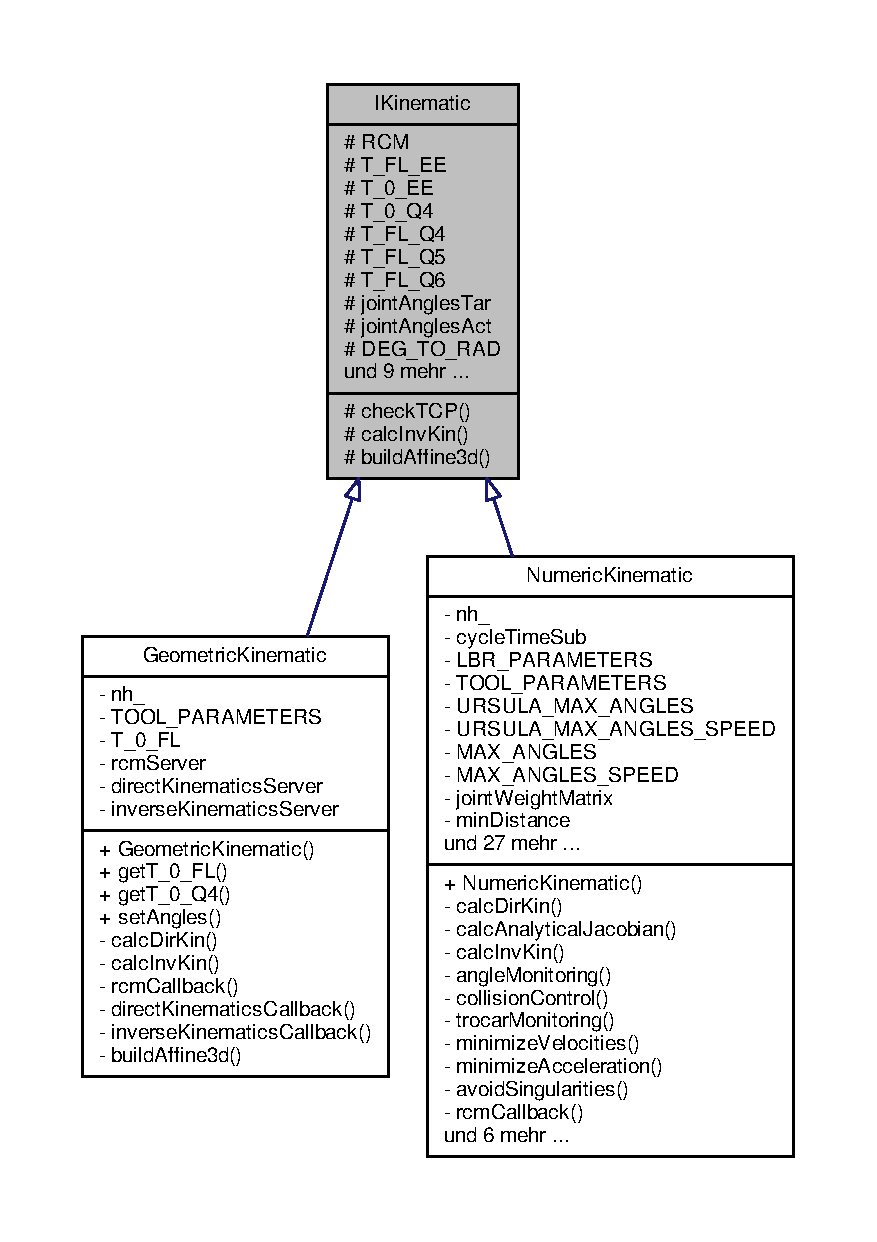
\includegraphics[width=350pt]{classIKinematic__inherit__graph}
\end{center}
\end{figure}


Zusammengehörigkeiten von I\-Kinematic\-:
\nopagebreak
\begin{figure}[H]
\begin{center}
\leavevmode
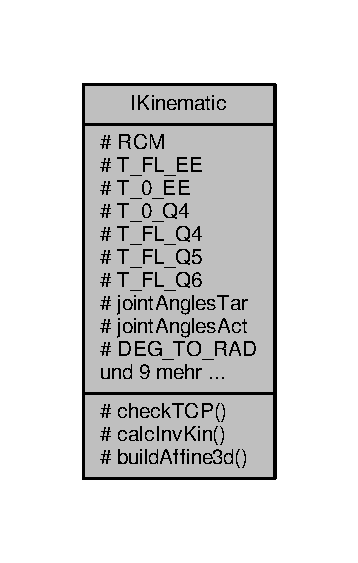
\includegraphics[width=172pt]{classIKinematic__coll__graph}
\end{center}
\end{figure}
\subsection*{Geschützte Methoden}
\begin{DoxyCompactItemize}
\item 
bool \hyperlink{classIKinematic_a2c740366fa7cca713fb0962a6be7e9f0}{check\-T\-C\-P} (Eigen\-::\-Affine3d T\-C\-P)
\begin{DoxyCompactList}\small\item\em Arbeitsraumüberwachung. \end{DoxyCompactList}\item 
virtual bool \hyperlink{classIKinematic_a6f95d80c4330253643c49a758404e4a7}{calc\-Inv\-Kin} (Eigen\-::\-Affine3d \hyperlink{classIKinematic_a1c0a95317992b7fcaf26ab2bf9aaf3de}{T\-\_\-0\-\_\-\-E\-E})=0
\begin{DoxyCompactList}\small\item\em Abstrakte Methode zur Berechnung der inversen Kinematik. \end{DoxyCompactList}\item 
Eigen\-::\-Affine3d \hyperlink{classIKinematic_af2065ef145ec1f796e5e34b123f4dd46}{build\-Affine3d} (const Eigen\-::\-Vector3d \&transl\-X\-Y\-Z, const Eigen\-::\-Vector3d \&axis\-Z\-Y\-X, bool zyx)
\begin{DoxyCompactList}\small\item\em Hilfsfunktion zur Erstellung von Affinen Transformationen aus einem Translationsvekt und den R\-P\-Y-\/\-Winkeln. \end{DoxyCompactList}\end{DoxyCompactItemize}
\subsection*{Geschützte Attribute}
\begin{DoxyCompactItemize}
\item 
\hypertarget{classIKinematic_a8aba9e0c27fc5f01b8eb93fa8afaf641}{Eigen\-::\-Affine3d \hyperlink{classIKinematic_a8aba9e0c27fc5f01b8eb93fa8afaf641}{R\-C\-M}}\label{classIKinematic_a8aba9e0c27fc5f01b8eb93fa8afaf641}

\begin{DoxyCompactList}\small\item\em Trokarpunkt im Weltkoordinatensystem. \end{DoxyCompactList}\item 
\hypertarget{classIKinematic_a04a66e41cfd8be035734e5c738df90e0}{Eigen\-::\-Affine3d \hyperlink{classIKinematic_a04a66e41cfd8be035734e5c738df90e0}{T\-\_\-\-F\-L\-\_\-\-E\-E}}\label{classIKinematic_a04a66e41cfd8be035734e5c738df90e0}

\begin{DoxyCompactList}\small\item\em Transformation zwischen Endeffektor und Roboterflansch. \end{DoxyCompactList}\item 
\hypertarget{classIKinematic_a1c0a95317992b7fcaf26ab2bf9aaf3de}{Eigen\-::\-Affine3d \hyperlink{classIKinematic_a1c0a95317992b7fcaf26ab2bf9aaf3de}{T\-\_\-0\-\_\-\-E\-E}}\label{classIKinematic_a1c0a95317992b7fcaf26ab2bf9aaf3de}

\begin{DoxyCompactList}\small\item\em Endeffektorlage im Weltkoordinatensystem. \end{DoxyCompactList}\item 
Eigen\-::\-Affine3d \hyperlink{classIKinematic_a0f3ae85bd946533cf8a22120f597ab00}{T\-\_\-0\-\_\-\-Q4}
\begin{DoxyCompactList}\small\item\em Lage des ersten Werkzeuggelenks im Weltkoordinatensystem. \end{DoxyCompactList}\item 
\hypertarget{classIKinematic_a45621d4e095f5b5ebd6b9eeae160e9fa}{Eigen\-::\-Affine3d \hyperlink{classIKinematic_a45621d4e095f5b5ebd6b9eeae160e9fa}{T\-\_\-\-F\-L\-\_\-\-Q4}}\label{classIKinematic_a45621d4e095f5b5ebd6b9eeae160e9fa}

\begin{DoxyCompactList}\small\item\em Lage des ersten Werkzeuggelenks im Roboterflanschkoordinatensystem. \end{DoxyCompactList}\item 
\hypertarget{classIKinematic_a40a738da633f12f257eb3e9f925cd00b}{Eigen\-::\-Affine3d \hyperlink{classIKinematic_a40a738da633f12f257eb3e9f925cd00b}{T\-\_\-\-F\-L\-\_\-\-Q5}}\label{classIKinematic_a40a738da633f12f257eb3e9f925cd00b}

\begin{DoxyCompactList}\small\item\em Lage des zweiten Werkzeuggelenks im Roboterflanschkoordinatensystem. \end{DoxyCompactList}\item 
\hypertarget{classIKinematic_a47670e07b24a57aabea5bbbb809eac03}{Eigen\-::\-Affine3d \hyperlink{classIKinematic_a47670e07b24a57aabea5bbbb809eac03}{T\-\_\-\-F\-L\-\_\-\-Q6}}\label{classIKinematic_a47670e07b24a57aabea5bbbb809eac03}

\begin{DoxyCompactList}\small\item\em Lage des dritten Werkzeuggelenks im Roboterflanschkoordinatensystem. \end{DoxyCompactList}\item 
\hypertarget{classIKinematic_aaac2e6408544098357a85b2b86ab25c3}{Eigen\-::\-Vector\-Xd \hyperlink{classIKinematic_aaac2e6408544098357a85b2b86ab25c3}{joint\-Angles\-Tar}}\label{classIKinematic_aaac2e6408544098357a85b2b86ab25c3}

\begin{DoxyCompactList}\small\item\em Vektor der gewünschten Gelenkwinkel des Werkzeuges bzw. des Gesamtsystems. \end{DoxyCompactList}\item 
\hypertarget{classIKinematic_ac262b75f38e66b1829585d398082fa10}{Eigen\-::\-Vector\-Xd \hyperlink{classIKinematic_ac262b75f38e66b1829585d398082fa10}{joint\-Angles\-Act}}\label{classIKinematic_ac262b75f38e66b1829585d398082fa10}

\begin{DoxyCompactList}\small\item\em Vektor der aktuellen Gelenkwinkel des Werkzeuges bzw. des Gesamtsystems. \end{DoxyCompactList}\item 
\hypertarget{classIKinematic_a37f44565aecbf830fa9c19b4fab672b2}{const double {\bfseries D\-E\-G\-\_\-\-T\-O\-\_\-\-R\-A\-D} \{M\-\_\-\-P\-I/180\}}\label{classIKinematic_a37f44565aecbf830fa9c19b4fab672b2}

\item 
\hypertarget{classIKinematic_ac41e50cd51191976b720a8ddd789188e}{const double {\bfseries M\-M\-\_\-\-T\-O\-\_\-\-M} \{1/1000\}}\label{classIKinematic_ac41e50cd51191976b720a8ddd789188e}

\item 
int \hyperlink{classIKinematic_a5b70ed8f56334c0ee5041e5eb787a056}{aperture\-Max} \{60\}
\item 
double \hyperlink{classIKinematic_a628b36a0331179b979468468c1efed54}{penetration\-Max} \{0.\-3\}
\item 
double \hyperlink{classIKinematic_a17905911cc852a855bd985bfda640ea2}{penetration\-Min} \{0.\-1\}
\item 
\hypertarget{classIKinematic_ad784d5dcc50b918c3b447e35b33d10e4}{bool \hyperlink{classIKinematic_ad784d5dcc50b918c3b447e35b33d10e4}{rcm\-Service\-Called} \{false\}}\label{classIKinematic_ad784d5dcc50b918c3b447e35b33d10e4}

\begin{DoxyCompactList}\small\item\em Flag, ob der Trokarpunkt berechnet ist. \end{DoxyCompactList}\item 
\hypertarget{classIKinematic_ad4984adc0630f9beaaebc83bc9b46bea}{bool \hyperlink{classIKinematic_ad4984adc0630f9beaaebc83bc9b46bea}{direct\-Kinematics\-Service\-Called} \{false\}}\label{classIKinematic_ad4984adc0630f9beaaebc83bc9b46bea}

\begin{DoxyCompactList}\small\item\em Flag, ob der aktuelle T\-C\-P bekannt ist. \end{DoxyCompactList}\item 
\hypertarget{classIKinematic_a98088de541bed2487314000b1b0c5e1c}{ros\-::\-Service\-Server \hyperlink{classIKinematic_a98088de541bed2487314000b1b0c5e1c}{rcm\-Service\-Server}}\label{classIKinematic_a98088de541bed2487314000b1b0c5e1c}

\begin{DoxyCompactList}\small\item\em Service\-Server für die Bestimmung des Trokarpunktes. \end{DoxyCompactList}\item 
\hypertarget{classIKinematic_a23847e7210bfeb2a62ad68de4a9ae6e1}{ros\-::\-Service\-Server \hyperlink{classIKinematic_a23847e7210bfeb2a62ad68de4a9ae6e1}{direct\-Kinematics\-Server}}\label{classIKinematic_a23847e7210bfeb2a62ad68de4a9ae6e1}

\begin{DoxyCompactList}\small\item\em Service\-Server für die Berechnung des T\-C\-P. \end{DoxyCompactList}\item 
\hypertarget{classIKinematic_acf7b1bf907b0f1a3f8d8aad56382c7a0}{ros\-::\-Service\-Server \hyperlink{classIKinematic_acf7b1bf907b0f1a3f8d8aad56382c7a0}{inverse\-Kinematics\-Server}}\label{classIKinematic_acf7b1bf907b0f1a3f8d8aad56382c7a0}

\begin{DoxyCompactList}\small\item\em Service\-Server für die Berechnung der Gelenkwinkel und der Roboterflanschlage im Weltkoordinatensystem. \end{DoxyCompactList}\end{DoxyCompactItemize}


\subsection{Ausführliche Beschreibung}
Abstrakte Basisklasse für die Kinematikberechnung. 

\begin{DoxyAuthor}{Autor}
Fabian Baier 
\end{DoxyAuthor}
\begin{DoxyDate}{Datum}
20.\-03.\-2016 
\end{DoxyDate}


\subsection{Dokumentation der Elementfunktionen}
\hypertarget{classIKinematic_af2065ef145ec1f796e5e34b123f4dd46}{\index{I\-Kinematic@{I\-Kinematic}!build\-Affine3d@{build\-Affine3d}}
\index{build\-Affine3d@{build\-Affine3d}!IKinematic@{I\-Kinematic}}
\subsubsection[{build\-Affine3d}]{\setlength{\rightskip}{0pt plus 5cm}I\-Kinematic\-::build\-Affine3d (
\begin{DoxyParamCaption}
\item[{const Eigen\-::\-Vector3d \&}]{transl\-X\-Y\-Z, }
\item[{const Eigen\-::\-Vector3d \&}]{axis\-Z\-Y\-X, }
\item[{bool}]{zyx}
\end{DoxyParamCaption}
)\hspace{0.3cm}{\ttfamily [protected]}}}\label{classIKinematic_af2065ef145ec1f796e5e34b123f4dd46}


Hilfsfunktion zur Erstellung von Affinen Transformationen aus einem Translationsvekt und den R\-P\-Y-\/\-Winkeln. 


\begin{DoxyParams}{Parameter}
{\em transl\-X\-Y\-Z} & Translationsvektor \\
\hline
{\em axis\-Z\-Y\-X} & Rotationsvektor \\
\hline
{\em zyx} & Flag zur Festlegung der Rotationsrichtung \\
\hline
\end{DoxyParams}
\begin{DoxyReturn}{Rückgabe}
Affine Transformation 
\end{DoxyReturn}
\hypertarget{classIKinematic_a6f95d80c4330253643c49a758404e4a7}{\index{I\-Kinematic@{I\-Kinematic}!calc\-Inv\-Kin@{calc\-Inv\-Kin}}
\index{calc\-Inv\-Kin@{calc\-Inv\-Kin}!IKinematic@{I\-Kinematic}}
\subsubsection[{calc\-Inv\-Kin}]{\setlength{\rightskip}{0pt plus 5cm}I\-Kinematic\-::calc\-Inv\-Kin (
\begin{DoxyParamCaption}
\item[{Eigen\-::\-Affine3d}]{T\-\_\-0\-\_\-\-E\-E}
\end{DoxyParamCaption}
)\hspace{0.3cm}{\ttfamily [protected]}, {\ttfamily [pure virtual]}}}\label{classIKinematic_a6f95d80c4330253643c49a758404e4a7}


Abstrakte Methode zur Berechnung der inversen Kinematik. 


\begin{DoxyParams}{Parameter}
{\em T\-\_\-0\-\_\-\-E\-E} & Aktuelle T\-C\-P-\/\-Lage \\
\hline
\end{DoxyParams}
\begin{DoxyReturn}{Rückgabe}
Arbeitsraumgrenzen eingehalten? 
\end{DoxyReturn}


Implementiert in \hyperlink{classGeometricKinematic_a40340db367bf2e3b10830c6ac54be302}{Geometric\-Kinematic} und \hyperlink{classNumericKinematic_a39d3e132f2d0786815cc9b5dc94f186a}{Numeric\-Kinematic}.

\hypertarget{classIKinematic_a2c740366fa7cca713fb0962a6be7e9f0}{\index{I\-Kinematic@{I\-Kinematic}!check\-T\-C\-P@{check\-T\-C\-P}}
\index{check\-T\-C\-P@{check\-T\-C\-P}!IKinematic@{I\-Kinematic}}
\subsubsection[{check\-T\-C\-P}]{\setlength{\rightskip}{0pt plus 5cm}I\-Kinematic\-::check\-T\-C\-P (
\begin{DoxyParamCaption}
\item[{Eigen\-::\-Affine3d}]{T\-C\-P}
\end{DoxyParamCaption}
)\hspace{0.3cm}{\ttfamily [protected]}}}\label{classIKinematic_a2c740366fa7cca713fb0962a6be7e9f0}


Arbeitsraumüberwachung. 

\begin{DoxyRefDesc}{Veraltet}
\item[\hyperlink{deprecated__deprecated000001}{Veraltet}]wird in der neuen Version entfernt, da es eigene Überwachungsklassen gibt 
\begin{DoxyParams}{Parameter}
{\em T\-C\-P} & Aktueller T\-C\-P \\
\hline
\end{DoxyParams}
\begin{DoxyReturn}{Rückgabe}
Flag, ob der definierte Arbeitsraum eingehalten wurde 
\end{DoxyReturn}
\begin{DoxySeeAlso}{Siehe auch}
\hyperlink{classBoundingBox}{Bounding\-Box} 
\end{DoxySeeAlso}
\end{DoxyRefDesc}


\subsection{Dokumentation der Datenelemente}
\hypertarget{classIKinematic_a5b70ed8f56334c0ee5041e5eb787a056}{\index{I\-Kinematic@{I\-Kinematic}!aperture\-Max@{aperture\-Max}}
\index{aperture\-Max@{aperture\-Max}!IKinematic@{I\-Kinematic}}
\subsubsection[{aperture\-Max}]{\setlength{\rightskip}{0pt plus 5cm}I\-Kinematic\-::aperture\-Max \{60\}\hspace{0.3cm}{\ttfamily [protected]}}}\label{classIKinematic_a5b70ed8f56334c0ee5041e5eb787a056}
\begin{DoxyRefDesc}{Veraltet}
\item[\hyperlink{deprecated__deprecated000002}{Veraltet}]\end{DoxyRefDesc}
\hypertarget{classIKinematic_a628b36a0331179b979468468c1efed54}{\index{I\-Kinematic@{I\-Kinematic}!penetration\-Max@{penetration\-Max}}
\index{penetration\-Max@{penetration\-Max}!IKinematic@{I\-Kinematic}}
\subsubsection[{penetration\-Max}]{\setlength{\rightskip}{0pt plus 5cm}I\-Kinematic\-::penetration\-Max \{0.\-3\}\hspace{0.3cm}{\ttfamily [protected]}}}\label{classIKinematic_a628b36a0331179b979468468c1efed54}
\begin{DoxyRefDesc}{Veraltet}
\item[\hyperlink{deprecated__deprecated000003}{Veraltet}]\end{DoxyRefDesc}
\hypertarget{classIKinematic_a17905911cc852a855bd985bfda640ea2}{\index{I\-Kinematic@{I\-Kinematic}!penetration\-Min@{penetration\-Min}}
\index{penetration\-Min@{penetration\-Min}!IKinematic@{I\-Kinematic}}
\subsubsection[{penetration\-Min}]{\setlength{\rightskip}{0pt plus 5cm}I\-Kinematic\-::penetration\-Min \{0.\-1\}\hspace{0.3cm}{\ttfamily [protected]}}}\label{classIKinematic_a17905911cc852a855bd985bfda640ea2}
\begin{DoxyRefDesc}{Veraltet}
\item[\hyperlink{deprecated__deprecated000004}{Veraltet}]\end{DoxyRefDesc}
\hypertarget{classIKinematic_a0f3ae85bd946533cf8a22120f597ab00}{\index{I\-Kinematic@{I\-Kinematic}!T\-\_\-0\-\_\-\-Q4@{T\-\_\-0\-\_\-\-Q4}}
\index{T\-\_\-0\-\_\-\-Q4@{T\-\_\-0\-\_\-\-Q4}!IKinematic@{I\-Kinematic}}
\subsubsection[{T\-\_\-0\-\_\-\-Q4}]{\setlength{\rightskip}{0pt plus 5cm}I\-Kinematic\-::\-T\-\_\-0\-\_\-\-Q4\hspace{0.3cm}{\ttfamily [protected]}}}\label{classIKinematic_a0f3ae85bd946533cf8a22120f597ab00}


Lage des ersten Werkzeuggelenks im Weltkoordinatensystem. 

\begin{DoxyRefDesc}{Noch zu erledigen}
\item[\hyperlink{todo__todo000011}{Noch zu erledigen}]Eindeutige Namenskonvention Q4tool und Q4lbr \end{DoxyRefDesc}


Die Dokumentation für diese Klasse wurde erzeugt aufgrund der Datei\-:\begin{DoxyCompactItemize}
\item 
include/masterslave/kinematic/\hyperlink{IKinematic_8h}{I\-Kinematic.\-h}\end{DoxyCompactItemize}

\hypertarget{classITrajectory}{\section{I\-Trajectory Klassenreferenz}
\label{classITrajectory}\index{I\-Trajectory@{I\-Trajectory}}
}


Abstrakte Basisklasse für verschiedene Trajektorienarten.  




{\ttfamily \#include $<$I\-Trajectory.\-h$>$}



Klassendiagramm für I\-Trajectory\-:
\nopagebreak
\begin{figure}[H]
\begin{center}
\leavevmode
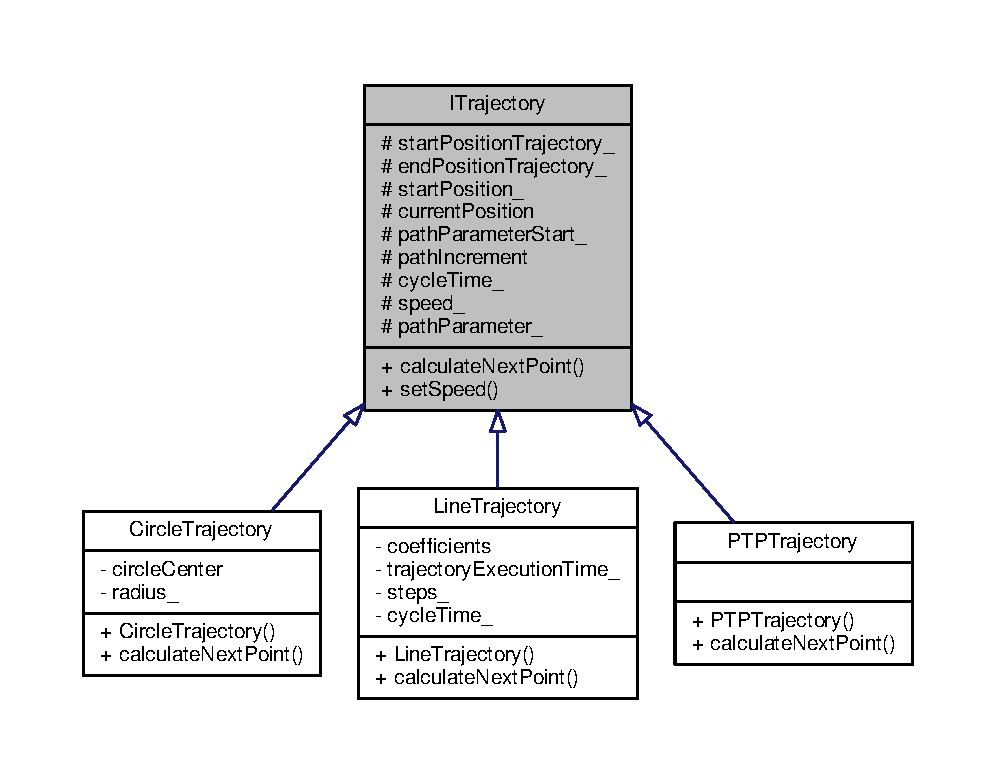
\includegraphics[width=350pt]{classITrajectory__inherit__graph}
\end{center}
\end{figure}


Zusammengehörigkeiten von I\-Trajectory\-:
\nopagebreak
\begin{figure}[H]
\begin{center}
\leavevmode
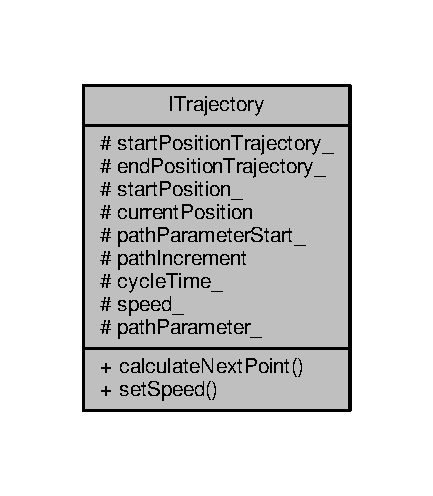
\includegraphics[width=208pt]{classITrajectory__coll__graph}
\end{center}
\end{figure}
\subsection*{Öffentliche Methoden}
\begin{DoxyCompactItemize}
\item 
virtual Eigen\-::\-Affine3d \hyperlink{classITrajectory_a7baff9fb2fc20987e9469d736a90406b}{calculate\-Next\-Point} ()=0
\begin{DoxyCompactList}\small\item\em Abstrakte Funktion zur Berechnung des nächsten Bahnpunktes. \end{DoxyCompactList}\item 
void \hyperlink{classITrajectory_a5067fb507df5d1e92249389325752fd6}{set\-Speed} (double speed)
\begin{DoxyCompactList}\small\item\em Zugriff auf die Bahngeschwindigkeit. \end{DoxyCompactList}\end{DoxyCompactItemize}
\subsection*{Geschützte Attribute}
\begin{DoxyCompactItemize}
\item 
Eigen\-::\-Affine3d \hyperlink{classITrajectory_a6884ba58490bcce750b698c2da8bc7bc}{start\-Position\-Trajectory\-\_\-}
\begin{DoxyCompactList}\small\item\em Startpunkt der gewünschten Trajektorie. \end{DoxyCompactList}\item 
Eigen\-::\-Affine3d \hyperlink{classITrajectory_ac49c42b8d8344554edb24d1ae525a64c}{end\-Position\-Trajectory\-\_\-}
\begin{DoxyCompactList}\small\item\em Endpunkt der gewünschten Trajektorie. \end{DoxyCompactList}\item 
Eigen\-::\-Affine3d \hyperlink{classITrajectory_a4fe5238f588ac3ed157bebf0dd7d45f5}{start\-Position\-\_\-}
\begin{DoxyCompactList}\small\item\em Aktuelle T\-C\-P-\/\-Lage und Startpunkt der P\-T\-P-\/\-Bewegung zu start\-Position\-Trajectory\-\_\-. \end{DoxyCompactList}\item 
Eigen\-::\-Affine3d \hyperlink{classITrajectory_ad0e7c293d6f0940523a158d4f898d366}{current\-Position}
\begin{DoxyCompactList}\small\item\em Aktuelle T\-C\-P-\/\-Lage während der Bahninterpolation. \end{DoxyCompactList}\item 
\hypertarget{classITrajectory_abd771a6cdd78a0a5bc188450c14057ff}{double \hyperlink{classITrajectory_abd771a6cdd78a0a5bc188450c14057ff}{path\-Parameter\-Start\-\_\-} \{0\}}\label{classITrajectory_abd771a6cdd78a0a5bc188450c14057ff}

\begin{DoxyCompactList}\small\item\em Pfadvariable der P\-T\-P-\/\-Bewegung zwischen start\-Position\-\_\- und start\-Position\-Trajectory\-\_\-. \end{DoxyCompactList}\item 
\hypertarget{classITrajectory_afa79f45c835319a41977e68cd711929c}{double \hyperlink{classITrajectory_afa79f45c835319a41977e68cd711929c}{path\-Increment}}\label{classITrajectory_afa79f45c835319a41977e68cd711929c}

\begin{DoxyCompactList}\small\item\em Der inkrementelle Teil der Bahn zwischen zwei Bahnpunkten. \end{DoxyCompactList}\item 
\hypertarget{classITrajectory_a04719c7e04b7c358e1a68cd5c9deba90}{double \hyperlink{classITrajectory_a04719c7e04b7c358e1a68cd5c9deba90}{cycle\-Time\-\_\-}}\label{classITrajectory_a04719c7e04b7c358e1a68cd5c9deba90}

\begin{DoxyCompactList}\small\item\em Zykluszeit. \end{DoxyCompactList}\item 
\hypertarget{classITrajectory_ab6ca758355699639b9210b55feb8de20}{double \hyperlink{classITrajectory_ab6ca758355699639b9210b55feb8de20}{speed\-\_\-}}\label{classITrajectory_ab6ca758355699639b9210b55feb8de20}

\begin{DoxyCompactList}\small\item\em Bahngeschwindigkeit in \mbox{[}mm/s\mbox{]}. \end{DoxyCompactList}\item 
\hypertarget{classITrajectory_adbe59ec29a3bc03f0d539cad15ccd935}{double \hyperlink{classITrajectory_adbe59ec29a3bc03f0d539cad15ccd935}{path\-Parameter\-\_\-} \{0\}}\label{classITrajectory_adbe59ec29a3bc03f0d539cad15ccd935}

\begin{DoxyCompactList}\small\item\em Pfadvariable der jeweiligen Trajektorie. \end{DoxyCompactList}\end{DoxyCompactItemize}


\subsection{Ausführliche Beschreibung}
Abstrakte Basisklasse für verschiedene Trajektorienarten. 

\begin{DoxyAuthor}{Autor}
Fabian Baier 
\end{DoxyAuthor}
\begin{DoxyDate}{Datum}
20.\-03.\-2016 
\end{DoxyDate}


\subsection{Dokumentation der Elementfunktionen}
\hypertarget{classITrajectory_a7baff9fb2fc20987e9469d736a90406b}{\index{I\-Trajectory@{I\-Trajectory}!calculate\-Next\-Point@{calculate\-Next\-Point}}
\index{calculate\-Next\-Point@{calculate\-Next\-Point}!ITrajectory@{I\-Trajectory}}
\subsubsection[{calculate\-Next\-Point}]{\setlength{\rightskip}{0pt plus 5cm}I\-Trajectory\-::calculate\-Next\-Point (
\begin{DoxyParamCaption}
{}
\end{DoxyParamCaption}
)\hspace{0.3cm}{\ttfamily [pure virtual]}}}\label{classITrajectory_a7baff9fb2fc20987e9469d736a90406b}


Abstrakte Funktion zur Berechnung des nächsten Bahnpunktes. 

\begin{DoxyReturn}{Rückgabe}
Nächster Bahnpunkt 
\end{DoxyReturn}


Implementiert in \hyperlink{classCircleTrajectory_a5629eff71ee01458eb8cdf7ad2b4b82f}{Circle\-Trajectory}, \hyperlink{classLineTrajectory_a94cbb5d8561ef9ea107b9faf8db89df5}{Line\-Trajectory} und \hyperlink{classPTPTrajectory_a6663a421aba9674577cdc014c8cb8b77}{P\-T\-P\-Trajectory}.

\hypertarget{classITrajectory_a5067fb507df5d1e92249389325752fd6}{\index{I\-Trajectory@{I\-Trajectory}!set\-Speed@{set\-Speed}}
\index{set\-Speed@{set\-Speed}!ITrajectory@{I\-Trajectory}}
\subsubsection[{set\-Speed}]{\setlength{\rightskip}{0pt plus 5cm}I\-Trajectory\-::set\-Speed (
\begin{DoxyParamCaption}
\item[{double}]{speed}
\end{DoxyParamCaption}
)\hspace{0.3cm}{\ttfamily [inline]}}}\label{classITrajectory_a5067fb507df5d1e92249389325752fd6}


Zugriff auf die Bahngeschwindigkeit. 


\begin{DoxyParams}{Parameter}
{\em speed} & Geschwindigkeit in \mbox{[}mm/s\mbox{]} \\
\hline
\end{DoxyParams}


\subsection{Dokumentation der Datenelemente}
\hypertarget{classITrajectory_ad0e7c293d6f0940523a158d4f898d366}{\index{I\-Trajectory@{I\-Trajectory}!current\-Position@{current\-Position}}
\index{current\-Position@{current\-Position}!ITrajectory@{I\-Trajectory}}
\subsubsection[{current\-Position}]{\setlength{\rightskip}{0pt plus 5cm}I\-Trajectory\-::current\-Position\hspace{0.3cm}{\ttfamily [protected]}}}\label{classITrajectory_ad0e7c293d6f0940523a158d4f898d366}


Aktuelle T\-C\-P-\/\-Lage während der Bahninterpolation. 

\begin{DoxySeeAlso}{Siehe auch}
\hyperlink{classITrajectory_a7baff9fb2fc20987e9469d736a90406b}{calculate\-Next\-Point} 
\end{DoxySeeAlso}
\hypertarget{classITrajectory_ac49c42b8d8344554edb24d1ae525a64c}{\index{I\-Trajectory@{I\-Trajectory}!end\-Position\-Trajectory\-\_\-@{end\-Position\-Trajectory\-\_\-}}
\index{end\-Position\-Trajectory\-\_\-@{end\-Position\-Trajectory\-\_\-}!ITrajectory@{I\-Trajectory}}
\subsubsection[{end\-Position\-Trajectory\-\_\-}]{\setlength{\rightskip}{0pt plus 5cm}I\-Trajectory\-::end\-Position\-Trajectory\-\_\-\hspace{0.3cm}{\ttfamily [protected]}}}\label{classITrajectory_ac49c42b8d8344554edb24d1ae525a64c}


Endpunkt der gewünschten Trajektorie. 

\begin{DoxySeeAlso}{Siehe auch}
\hyperlink{classITrajectory_a7baff9fb2fc20987e9469d736a90406b}{calculate\-Next\-Point} 
\end{DoxySeeAlso}
\hypertarget{classITrajectory_a4fe5238f588ac3ed157bebf0dd7d45f5}{\index{I\-Trajectory@{I\-Trajectory}!start\-Position\-\_\-@{start\-Position\-\_\-}}
\index{start\-Position\-\_\-@{start\-Position\-\_\-}!ITrajectory@{I\-Trajectory}}
\subsubsection[{start\-Position\-\_\-}]{\setlength{\rightskip}{0pt plus 5cm}I\-Trajectory\-::start\-Position\-\_\-\hspace{0.3cm}{\ttfamily [protected]}}}\label{classITrajectory_a4fe5238f588ac3ed157bebf0dd7d45f5}


Aktuelle T\-C\-P-\/\-Lage und Startpunkt der P\-T\-P-\/\-Bewegung zu start\-Position\-Trajectory\-\_\-. 

\begin{DoxySeeAlso}{Siehe auch}
\hyperlink{classITrajectory_a7baff9fb2fc20987e9469d736a90406b}{calculate\-Next\-Point} 
\end{DoxySeeAlso}
\hypertarget{classITrajectory_a6884ba58490bcce750b698c2da8bc7bc}{\index{I\-Trajectory@{I\-Trajectory}!start\-Position\-Trajectory\-\_\-@{start\-Position\-Trajectory\-\_\-}}
\index{start\-Position\-Trajectory\-\_\-@{start\-Position\-Trajectory\-\_\-}!ITrajectory@{I\-Trajectory}}
\subsubsection[{start\-Position\-Trajectory\-\_\-}]{\setlength{\rightskip}{0pt plus 5cm}I\-Trajectory\-::start\-Position\-Trajectory\-\_\-\hspace{0.3cm}{\ttfamily [protected]}}}\label{classITrajectory_a6884ba58490bcce750b698c2da8bc7bc}


Startpunkt der gewünschten Trajektorie. 

\begin{DoxySeeAlso}{Siehe auch}
\hyperlink{classITrajectory_a7baff9fb2fc20987e9469d736a90406b}{calculate\-Next\-Point} 
\end{DoxySeeAlso}


Die Dokumentation für diese Klasse wurde erzeugt aufgrund der Datei\-:\begin{DoxyCompactItemize}
\item 
include/masterslave/manipulation/trajectory/\hyperlink{ITrajectory_8h}{I\-Trajectory.\-h}\end{DoxyCompactItemize}

\hypertarget{structlbrDescriptionParameters}{\section{lbr\-Description\-Parameters Strukturreferenz}
\label{structlbrDescriptionParameters}\index{lbr\-Description\-Parameters@{lbr\-Description\-Parameters}}
}


Zusammengehörigkeiten von lbr\-Description\-Parameters\-:
\nopagebreak
\begin{figure}[H]
\begin{center}
\leavevmode
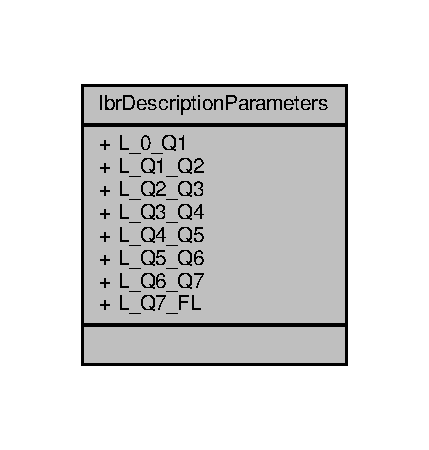
\includegraphics[width=206pt]{structlbrDescriptionParameters__coll__graph}
\end{center}
\end{figure}
\subsection*{Öffentliche Attribute}
\begin{DoxyCompactItemize}
\item 
\hypertarget{structlbrDescriptionParameters_a70c50b164fcca4c27ec244a83714f6f3}{const double {\bfseries L\-\_\-0\-\_\-\-Q1}}\label{structlbrDescriptionParameters_a70c50b164fcca4c27ec244a83714f6f3}

\item 
\hypertarget{structlbrDescriptionParameters_af73f716fc6eaabf5ec13e07fa4f1eee3}{const double {\bfseries L\-\_\-\-Q1\-\_\-\-Q2}}\label{structlbrDescriptionParameters_af73f716fc6eaabf5ec13e07fa4f1eee3}

\item 
\hypertarget{structlbrDescriptionParameters_aad77a7879ffd39d37b3b6ee4915fd682}{const double {\bfseries L\-\_\-\-Q2\-\_\-\-Q3}}\label{structlbrDescriptionParameters_aad77a7879ffd39d37b3b6ee4915fd682}

\item 
\hypertarget{structlbrDescriptionParameters_ab34af085c26de98917c9a5cf7299c0b0}{const double {\bfseries L\-\_\-\-Q3\-\_\-\-Q4}}\label{structlbrDescriptionParameters_ab34af085c26de98917c9a5cf7299c0b0}

\item 
\hypertarget{structlbrDescriptionParameters_a80b3afbe09aa3c9837e6fd86f9036eb4}{const double {\bfseries L\-\_\-\-Q4\-\_\-\-Q5}}\label{structlbrDescriptionParameters_a80b3afbe09aa3c9837e6fd86f9036eb4}

\item 
\hypertarget{structlbrDescriptionParameters_a16e9ac758d9e1d7210133e69f7f1157d}{const double {\bfseries L\-\_\-\-Q5\-\_\-\-Q6}}\label{structlbrDescriptionParameters_a16e9ac758d9e1d7210133e69f7f1157d}

\item 
\hypertarget{structlbrDescriptionParameters_a6c3087fb2839875c17c28275b5e411b0}{const double {\bfseries L\-\_\-\-Q6\-\_\-\-Q7}}\label{structlbrDescriptionParameters_a6c3087fb2839875c17c28275b5e411b0}

\item 
\hypertarget{structlbrDescriptionParameters_a417e5478d67dedb0feea59594d531683}{const double {\bfseries L\-\_\-\-Q7\-\_\-\-F\-L}}\label{structlbrDescriptionParameters_a417e5478d67dedb0feea59594d531683}

\end{DoxyCompactItemize}


Die Dokumentation für diese Struktur wurde erzeugt aufgrund der Datei\-:\begin{DoxyCompactItemize}
\item 
include/masterslave/Description\-Parameters.\-h\end{DoxyCompactItemize}

\hypertarget{structlbrJointAngles}{\section{lbr\-Joint\-Angles Strukturreferenz}
\label{structlbrJointAngles}\index{lbr\-Joint\-Angles@{lbr\-Joint\-Angles}}
}


Zusammengehörigkeiten von lbr\-Joint\-Angles\-:
\nopagebreak
\begin{figure}[H]
\begin{center}
\leavevmode
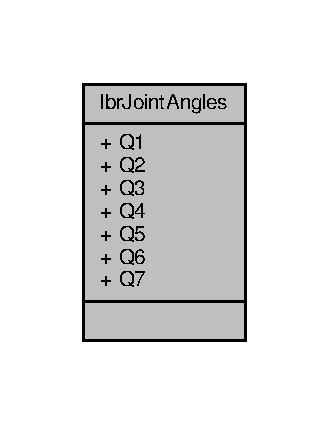
\includegraphics[width=158pt]{structlbrJointAngles__coll__graph}
\end{center}
\end{figure}
\subsection*{Öffentliche Attribute}
\begin{DoxyCompactItemize}
\item 
\hypertarget{structlbrJointAngles_a18069e0505c332f0be822ae6bbfad263}{double {\bfseries Q1}}\label{structlbrJointAngles_a18069e0505c332f0be822ae6bbfad263}

\item 
\hypertarget{structlbrJointAngles_a5e25dfb7253b5cef4c4d6116eab50f19}{double {\bfseries Q2}}\label{structlbrJointAngles_a5e25dfb7253b5cef4c4d6116eab50f19}

\item 
\hypertarget{structlbrJointAngles_a2b8455d90c29b5fbfc5bea327b70d997}{double {\bfseries Q3}}\label{structlbrJointAngles_a2b8455d90c29b5fbfc5bea327b70d997}

\item 
\hypertarget{structlbrJointAngles_aa0203dcf13361ce8db6d8c6d3a6ffba0}{double {\bfseries Q4}}\label{structlbrJointAngles_aa0203dcf13361ce8db6d8c6d3a6ffba0}

\item 
\hypertarget{structlbrJointAngles_a74d22803618cfb8ed2c1aac61d72a368}{double {\bfseries Q5}}\label{structlbrJointAngles_a74d22803618cfb8ed2c1aac61d72a368}

\item 
\hypertarget{structlbrJointAngles_a1565744be30b2b453bd8f1b44216732e}{double {\bfseries Q6}}\label{structlbrJointAngles_a1565744be30b2b453bd8f1b44216732e}

\item 
\hypertarget{structlbrJointAngles_acc334be5fb62073fc40a7b188fbc44cc}{double {\bfseries Q7}}\label{structlbrJointAngles_acc334be5fb62073fc40a7b188fbc44cc}

\end{DoxyCompactItemize}


Die Dokumentation für diese Struktur wurde erzeugt aufgrund der Datei\-:\begin{DoxyCompactItemize}
\item 
include/masterslave/Description\-Parameters.\-h\end{DoxyCompactItemize}

\hypertarget{classLineTrajectory}{\section{Line\-Trajectory Klassenreferenz}
\label{classLineTrajectory}\index{Line\-Trajectory@{Line\-Trajectory}}
}


Eine Klasse, die eine Interpolation eines Polynom fünften Grades zwischen zwei Punkten ermöglicht.  




{\ttfamily \#include $<$Line\-Trajectory.\-h$>$}



Klassendiagramm für Line\-Trajectory\-:
\nopagebreak
\begin{figure}[H]
\begin{center}
\leavevmode
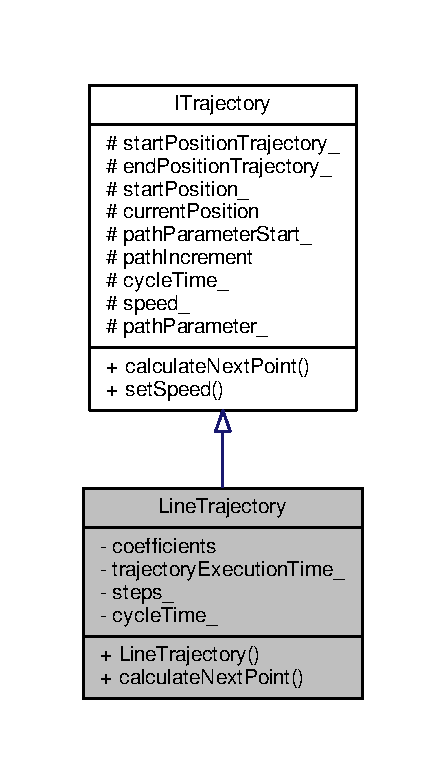
\includegraphics[width=214pt]{classLineTrajectory__inherit__graph}
\end{center}
\end{figure}


Zusammengehörigkeiten von Line\-Trajectory\-:
\nopagebreak
\begin{figure}[H]
\begin{center}
\leavevmode
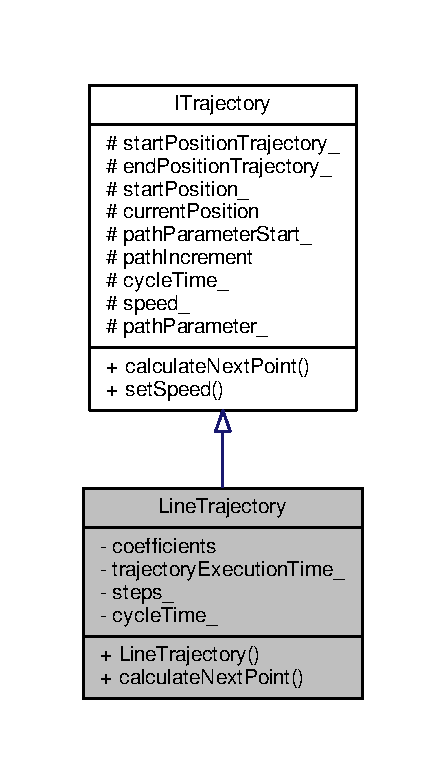
\includegraphics[width=214pt]{classLineTrajectory__coll__graph}
\end{center}
\end{figure}
\subsection*{Öffentliche Methoden}
\begin{DoxyCompactItemize}
\item 
\hypertarget{classLineTrajectory_a4d872310cac1add21fe99132f8ed596e}{{\bfseries Line\-Trajectory} (Eigen\-::\-Affine3d start\-Position, Eigen\-::\-Vector3d R\-C\-M, Eigen\-::\-Vector3d first\-Point, Eigen\-::\-Vector3d second\-Point, int speed, double cycle\-Time)}\label{classLineTrajectory_a4d872310cac1add21fe99132f8ed596e}

\item 
Eigen\-::\-Affine3d \hyperlink{classLineTrajectory_a94cbb5d8561ef9ea107b9faf8db89df5}{calculate\-Next\-Point} ()
\end{DoxyCompactItemize}
\subsection*{Private Attribute}
\begin{DoxyCompactItemize}
\item 
\hypertarget{classLineTrajectory_a560c794ebfff602aad735b931c132963}{std\-::array$<$ Eigen\-::\-Vector3d, 6 $>$ \hyperlink{classLineTrajectory_a560c794ebfff602aad735b931c132963}{coefficients}}\label{classLineTrajectory_a560c794ebfff602aad735b931c132963}

\begin{DoxyCompactList}\small\item\em Koeffizienten des Polynoms fünften Grades. \end{DoxyCompactList}\item 
\hypertarget{classLineTrajectory_a983b6fea1e70c24aa8d1aa7770d3ff66}{double \hyperlink{classLineTrajectory_a983b6fea1e70c24aa8d1aa7770d3ff66}{trajectory\-Execution\-Time\-\_\-}}\label{classLineTrajectory_a983b6fea1e70c24aa8d1aa7770d3ff66}

\begin{DoxyCompactList}\small\item\em Zeit für die Interpolation zwischen den zwei Punkten in Abhängigkeit der gewünschten durchschnittlichen Geschwindigkeit. \end{DoxyCompactList}\item 
\hypertarget{classLineTrajectory_a763e4b203bed598f8e258bada6a1a008}{int \hyperlink{classLineTrajectory_a763e4b203bed598f8e258bada6a1a008}{steps\-\_\-}}\label{classLineTrajectory_a763e4b203bed598f8e258bada6a1a008}

\begin{DoxyCompactList}\small\item\em Anzahl der Interpolationsschritte in Abhängigkeit der Länge der Trajektore, der Bahngeschwindigkeit und der Zykluszeit. \end{DoxyCompactList}\item 
\hypertarget{classLineTrajectory_a14bddd082451c9c5a33141d9fa6816f6}{double \hyperlink{classLineTrajectory_a14bddd082451c9c5a33141d9fa6816f6}{cycle\-Time\-\_\-}}\label{classLineTrajectory_a14bddd082451c9c5a33141d9fa6816f6}

\begin{DoxyCompactList}\small\item\em Zykluszeit. \end{DoxyCompactList}\end{DoxyCompactItemize}
\subsection*{Weitere Geerbte Elemente}


\subsection{Ausführliche Beschreibung}
Eine Klasse, die eine Interpolation eines Polynom fünften Grades zwischen zwei Punkten ermöglicht. 

\begin{DoxyAuthor}{Autor}
Fabian Baier 
\end{DoxyAuthor}
\begin{DoxyDate}{Datum}
20.\-03.\-2016 
\end{DoxyDate}


\subsection{Dokumentation der Elementfunktionen}
\hypertarget{classLineTrajectory_a94cbb5d8561ef9ea107b9faf8db89df5}{\index{Line\-Trajectory@{Line\-Trajectory}!calculate\-Next\-Point@{calculate\-Next\-Point}}
\index{calculate\-Next\-Point@{calculate\-Next\-Point}!LineTrajectory@{Line\-Trajectory}}
\subsubsection[{calculate\-Next\-Point}]{\setlength{\rightskip}{0pt plus 5cm}Line\-Trajectory\-::calculate\-Next\-Point (
\begin{DoxyParamCaption}
{}
\end{DoxyParamCaption}
)\hspace{0.3cm}{\ttfamily [virtual]}}}\label{classLineTrajectory_a94cbb5d8561ef9ea107b9faf8db89df5}
\begin{DoxySeeAlso}{Siehe auch}
\hyperlink{classITrajectory}{I\-Trajectory} 
\end{DoxySeeAlso}


Implementiert \hyperlink{classITrajectory_a7baff9fb2fc20987e9469d736a90406b}{I\-Trajectory}.



Die Dokumentation für diese Klasse wurde erzeugt aufgrund der Datei\-:\begin{DoxyCompactItemize}
\item 
include/masterslave/manipulation/trajectory/\hyperlink{LineTrajectory_8h}{Line\-Trajectory.\-h}\end{DoxyCompactItemize}

\hypertarget{classMasterSlave}{\section{Master\-Slave Klassenreferenz}
\label{classMasterSlave}\index{Master\-Slave@{Master\-Slave}}
}


Zusammengehörigkeiten von Master\-Slave\-:
\nopagebreak
\begin{figure}[H]
\begin{center}
\leavevmode
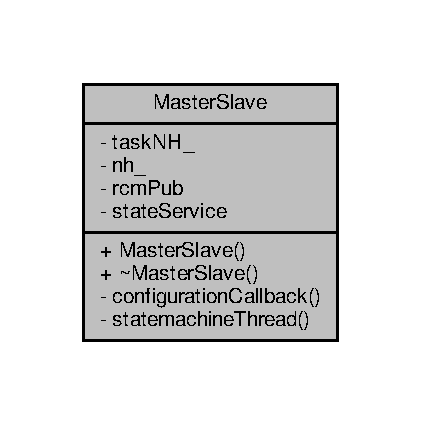
\includegraphics[width=202pt]{classMasterSlave__coll__graph}
\end{center}
\end{figure}
\subsection*{Öffentliche Methoden}
\begin{DoxyCompactItemize}
\item 
\hypertarget{classMasterSlave_ab5290259fb581b7742a37db37a6a4137}{{\bfseries Master\-Slave} (ros\-::\-Node\-Handle \&, ros\-::\-Node\-Handle \&)}\label{classMasterSlave_ab5290259fb581b7742a37db37a6a4137}

\end{DoxyCompactItemize}
\subsection*{Private Methoden}
\begin{DoxyCompactItemize}
\item 
\hypertarget{classMasterSlave_ac61a3fde8040d7467d64ee0fbdb3421a}{void {\bfseries configuration\-Callback} (masterslave\-::\-Master\-Slave\-Config \&config, uint32\-\_\-t level)}\label{classMasterSlave_ac61a3fde8040d7467d64ee0fbdb3421a}

\item 
\hypertarget{classMasterSlave_a3085b599a52c3d3f08fce578699e9fb1}{void {\bfseries statemachine\-Thread} (const ros\-::\-Timer\-Event \&)}\label{classMasterSlave_a3085b599a52c3d3f08fce578699e9fb1}

\end{DoxyCompactItemize}
\subsection*{Private Attribute}
\begin{DoxyCompactItemize}
\item 
\hypertarget{classMasterSlave_a3d15a95210336763c63ac75cc31b0082}{ros\-::\-Node\-Handle {\bfseries task\-N\-H\-\_\-}}\label{classMasterSlave_a3d15a95210336763c63ac75cc31b0082}

\item 
\hypertarget{classMasterSlave_acc17666bfd856c32ad2ca08cea37683c}{ros\-::\-Node\-Handle {\bfseries nh\-\_\-}}\label{classMasterSlave_acc17666bfd856c32ad2ca08cea37683c}

\item 
\hypertarget{classMasterSlave_a3742cdbfc7a31e08d396816d8e1704bb}{ros\-::\-Publisher {\bfseries rcm\-Pub}}\label{classMasterSlave_a3742cdbfc7a31e08d396816d8e1704bb}

\item 
\hypertarget{classMasterSlave_a5a059116c10d34fd2cd70ff2f479cb55}{ros\-::\-Service\-Client {\bfseries state\-Service}}\label{classMasterSlave_a5a059116c10d34fd2cd70ff2f479cb55}

\end{DoxyCompactItemize}


Die Dokumentation für diese Klasse wurde erzeugt aufgrund der Datei\-:\begin{DoxyCompactItemize}
\item 
include/masterslave/Master\-Slave.\-h\end{DoxyCompactItemize}

\hypertarget{classMasterSlaveManipulation}{\section{Master\-Slave\-Manipulation Klassenreferenz}
\label{classMasterSlaveManipulation}\index{Master\-Slave\-Manipulation@{Master\-Slave\-Manipulation}}
}


Klasse, die sich um die Manipulation des T\-C\-P mittels des Eingabegerätes kümmert.  




{\ttfamily \#include $<$Master\-Slave\-Manipulation.\-h$>$}



Zusammengehörigkeiten von Master\-Slave\-Manipulation\-:
\nopagebreak
\begin{figure}[H]
\begin{center}
\leavevmode
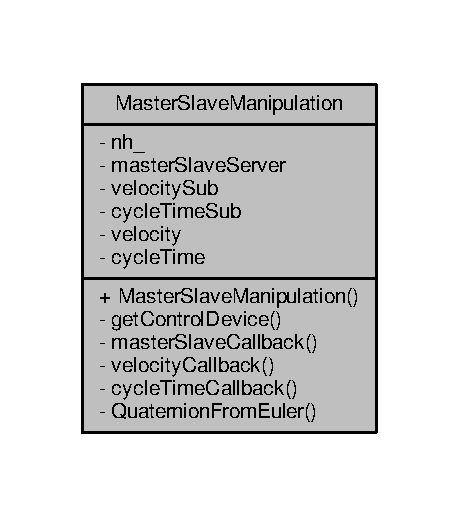
\includegraphics[width=220pt]{classMasterSlaveManipulation__coll__graph}
\end{center}
\end{figure}
\subsection*{Öffentliche Methoden}
\begin{DoxyCompactItemize}
\item 
\hypertarget{classMasterSlaveManipulation_a7f517d59d59a8d27d905b36edc604715}{{\bfseries Master\-Slave\-Manipulation} (ros\-::\-Node\-Handle \&nh)}\label{classMasterSlaveManipulation_a7f517d59d59a8d27d905b36edc604715}

\end{DoxyCompactItemize}
\subsection*{Private Methoden}
\begin{DoxyCompactItemize}
\item 
\hypertarget{classMasterSlaveManipulation_a65c146773e36828ea63e177e8d03017e}{void \hyperlink{classMasterSlaveManipulation_a65c146773e36828ea63e177e8d03017e}{get\-Control\-Device} ()}\label{classMasterSlaveManipulation_a65c146773e36828ea63e177e8d03017e}

\begin{DoxyCompactList}\small\item\em Die Methode liest das Eingabegerät vom Parameterserver aus. \end{DoxyCompactList}\item 
bool \hyperlink{classMasterSlaveManipulation_a142d1ec4b3126540a6bce1998452d0af}{master\-Slave\-Callback} (masterslave\-::\-Manipulation\-::\-Request \&req, masterslave\-::\-Manipulation\-::\-Response \&resp)
\begin{DoxyCompactList}\small\item\em Manipulation Service Callbackmethode. \end{DoxyCompactList}\item 
\hypertarget{classMasterSlaveManipulation_adfd18bc0bb7cdd93586aca7aaea2c696}{void \hyperlink{classMasterSlaveManipulation_adfd18bc0bb7cdd93586aca7aaea2c696}{velocity\-Callback} (const geometry\-\_\-msgs\-::\-Twist\-Stamped\-Const\-Ptr \&)}\label{classMasterSlaveManipulation_adfd18bc0bb7cdd93586aca7aaea2c696}

\begin{DoxyCompactList}\small\item\em Callbackmethode in der die Achswerte des Eingabegerätes ausgelesen werden. \end{DoxyCompactList}\item 
\hypertarget{classMasterSlaveManipulation_a3030f547b0e41511315948b020912230}{void \hyperlink{classMasterSlaveManipulation_a3030f547b0e41511315948b020912230}{cycle\-Time\-Callback} (const std\-\_\-msgs\-::\-Float64\-Const\-Ptr \&)}\label{classMasterSlaveManipulation_a3030f547b0e41511315948b020912230}

\begin{DoxyCompactList}\small\item\em Callback zum Empfang der Zykluszeit. \end{DoxyCompactList}\item 
Eigen\-::\-Quaternion$<$ double $>$ \hyperlink{classMasterSlaveManipulation_a09a4d65773ae287f0bf16bb0d8b26791}{Quaternion\-From\-Euler} (const Eigen\-::\-Vector3d \&euler\-X\-Y\-Z, bool Z\-Y\-X)
\begin{DoxyCompactList}\small\item\em Hilfsfunktion zur Wandlung eines Euler-\/\-Winkel-\/\-Vektors in ein Quaternions. \end{DoxyCompactList}\end{DoxyCompactItemize}
\subsection*{Private Attribute}
\begin{DoxyCompactItemize}
\item 
\hypertarget{classMasterSlaveManipulation_a958d5aeb711682d6dc180631f39961fa}{ros\-::\-Node\-Handle {\bfseries nh\-\_\-}}\label{classMasterSlaveManipulation_a958d5aeb711682d6dc180631f39961fa}

\item 
ros\-::\-Service\-Server \hyperlink{classMasterSlaveManipulation_ad9ecf87702f7a462130fdb48fe3e8df2}{master\-Slave\-Server}
\begin{DoxyCompactList}\small\item\em Service Server zur Bereitstellung des Master-\/\-Slave-\/\-Service. \end{DoxyCompactList}\item 
ros\-::\-Subscriber \hyperlink{classMasterSlaveManipulation_ab7809d9d1d1b96530ca9aec2d10a0fab}{velocity\-Sub}
\begin{DoxyCompactList}\small\item\em Empfänger des Achsvektors des Eingabegerätes. \end{DoxyCompactList}\item 
ros\-::\-Subscriber \hyperlink{classMasterSlaveManipulation_ac8952201baad0d7dbc0d4e22b519ef70}{cycle\-Time\-Sub}
\begin{DoxyCompactList}\small\item\em Empfänger für die Zykluszeit. \end{DoxyCompactList}\item 
\hypertarget{classMasterSlaveManipulation_a75bc6790c25f850d5047b5b4217834fd}{geometry\-\_\-msgs\-::\-Twist\-Stamped \hyperlink{classMasterSlaveManipulation_a75bc6790c25f850d5047b5b4217834fd}{velocity}}\label{classMasterSlaveManipulation_a75bc6790c25f850d5047b5b4217834fd}

\begin{DoxyCompactList}\small\item\em Vorheriger Achsvektor des Eingabegerätes. \end{DoxyCompactList}\item 
\hypertarget{classMasterSlaveManipulation_a395fee7bb621b884b79f20e81a1934fc}{double \hyperlink{classMasterSlaveManipulation_a395fee7bb621b884b79f20e81a1934fc}{cycle\-Time}}\label{classMasterSlaveManipulation_a395fee7bb621b884b79f20e81a1934fc}

\begin{DoxyCompactList}\small\item\em Zykluszeit. \end{DoxyCompactList}\end{DoxyCompactItemize}


\subsection{Ausführliche Beschreibung}
Klasse, die sich um die Manipulation des T\-C\-P mittels des Eingabegerätes kümmert. 

\begin{DoxyAuthor}{Autor}
Fabian Baier 
\end{DoxyAuthor}
\begin{DoxyDate}{Datum}
20.\-03.\-2016 
\end{DoxyDate}


\subsection{Dokumentation der Elementfunktionen}
\hypertarget{classMasterSlaveManipulation_a142d1ec4b3126540a6bce1998452d0af}{\index{Master\-Slave\-Manipulation@{Master\-Slave\-Manipulation}!master\-Slave\-Callback@{master\-Slave\-Callback}}
\index{master\-Slave\-Callback@{master\-Slave\-Callback}!MasterSlaveManipulation@{Master\-Slave\-Manipulation}}
\subsubsection[{master\-Slave\-Callback}]{\setlength{\rightskip}{0pt plus 5cm}Master\-Slave\-Manipulation\-::master\-Slave\-Callback (
\begin{DoxyParamCaption}
\item[{masterslave\-::\-Manipulation\-::\-Request \&}]{req, }
\item[{masterslave\-::\-Manipulation\-::\-Response \&}]{resp}
\end{DoxyParamCaption}
)\hspace{0.3cm}{\ttfamily [private]}}}\label{classMasterSlaveManipulation_a142d1ec4b3126540a6bce1998452d0af}


Manipulation Service Callbackmethode. 


\begin{DoxyParams}{Parameter}
{\em req} & Alter T\-C\-P vor der Manipulation \\
\hline
{\em resp} & Neuer T\-C\-P nach der Manipulation \\
\hline
\end{DoxyParams}
\begin{DoxyReturn}{Rückgabe}
Flag, die den Erfolg des Service Calls anzeigt 
\end{DoxyReturn}
\hypertarget{classMasterSlaveManipulation_a09a4d65773ae287f0bf16bb0d8b26791}{\index{Master\-Slave\-Manipulation@{Master\-Slave\-Manipulation}!Quaternion\-From\-Euler@{Quaternion\-From\-Euler}}
\index{Quaternion\-From\-Euler@{Quaternion\-From\-Euler}!MasterSlaveManipulation@{Master\-Slave\-Manipulation}}
\subsubsection[{Quaternion\-From\-Euler}]{\setlength{\rightskip}{0pt plus 5cm}Master\-Slave\-Manipulation\-::\-Quaternion\-From\-Euler (
\begin{DoxyParamCaption}
\item[{const Eigen\-::\-Vector3d \&}]{euler\-X\-Y\-Z, }
\item[{bool}]{Z\-Y\-X}
\end{DoxyParamCaption}
)\hspace{0.3cm}{\ttfamily [private]}}}\label{classMasterSlaveManipulation_a09a4d65773ae287f0bf16bb0d8b26791}


Hilfsfunktion zur Wandlung eines Euler-\/\-Winkel-\/\-Vektors in ein Quaternions. 


\begin{DoxyParams}{Parameter}
{\em euler\-X\-Y\-Z} & Euler-\/\-Winkel-\/\-Vektor \\
\hline
{\em Z\-Y\-X} & Flag, zur Festlegung der Rotationsreihenfolge \\
\hline
\end{DoxyParams}
\begin{DoxyReturn}{Rückgabe}
Quaternion 
\end{DoxyReturn}


\subsection{Dokumentation der Datenelemente}
\hypertarget{classMasterSlaveManipulation_ac8952201baad0d7dbc0d4e22b519ef70}{\index{Master\-Slave\-Manipulation@{Master\-Slave\-Manipulation}!cycle\-Time\-Sub@{cycle\-Time\-Sub}}
\index{cycle\-Time\-Sub@{cycle\-Time\-Sub}!MasterSlaveManipulation@{Master\-Slave\-Manipulation}}
\subsubsection[{cycle\-Time\-Sub}]{\setlength{\rightskip}{0pt plus 5cm}Master\-Slave\-Manipulation\-::cycle\-Time\-Sub\hspace{0.3cm}{\ttfamily [private]}}}\label{classMasterSlaveManipulation_ac8952201baad0d7dbc0d4e22b519ef70}


Empfänger für die Zykluszeit. 

\begin{DoxySeeAlso}{Siehe auch}
\hyperlink{classMasterSlaveManipulation_a3030f547b0e41511315948b020912230}{cycle\-Time\-Callback} 
\end{DoxySeeAlso}
\hypertarget{classMasterSlaveManipulation_ad9ecf87702f7a462130fdb48fe3e8df2}{\index{Master\-Slave\-Manipulation@{Master\-Slave\-Manipulation}!master\-Slave\-Server@{master\-Slave\-Server}}
\index{master\-Slave\-Server@{master\-Slave\-Server}!MasterSlaveManipulation@{Master\-Slave\-Manipulation}}
\subsubsection[{master\-Slave\-Server}]{\setlength{\rightskip}{0pt plus 5cm}Master\-Slave\-Manipulation\-::master\-Slave\-Server\hspace{0.3cm}{\ttfamily [private]}}}\label{classMasterSlaveManipulation_ad9ecf87702f7a462130fdb48fe3e8df2}


Service Server zur Bereitstellung des Master-\/\-Slave-\/\-Service. 

\begin{DoxySeeAlso}{Siehe auch}
Master\-Slave.\-srv 
\end{DoxySeeAlso}
\hypertarget{classMasterSlaveManipulation_ab7809d9d1d1b96530ca9aec2d10a0fab}{\index{Master\-Slave\-Manipulation@{Master\-Slave\-Manipulation}!velocity\-Sub@{velocity\-Sub}}
\index{velocity\-Sub@{velocity\-Sub}!MasterSlaveManipulation@{Master\-Slave\-Manipulation}}
\subsubsection[{velocity\-Sub}]{\setlength{\rightskip}{0pt plus 5cm}Master\-Slave\-Manipulation\-::velocity\-Sub\hspace{0.3cm}{\ttfamily [private]}}}\label{classMasterSlaveManipulation_ab7809d9d1d1b96530ca9aec2d10a0fab}


Empfänger des Achsvektors des Eingabegerätes. 

\begin{DoxySeeAlso}{Siehe auch}
\hyperlink{classMasterSlaveManipulation_adfd18bc0bb7cdd93586aca7aaea2c696}{velocity\-Callback} 
\end{DoxySeeAlso}


Die Dokumentation für diese Klasse wurde erzeugt aufgrund der Datei\-:\begin{DoxyCompactItemize}
\item 
include/masterslave/manipulation/\hyperlink{MasterSlaveManipulation_8h}{Master\-Slave\-Manipulation.\-h}\end{DoxyCompactItemize}

\hypertarget{classNumericKinematic}{\section{Numeric\-Kinematic Klassenreferenz}
\label{classNumericKinematic}\index{Numeric\-Kinematic@{Numeric\-Kinematic}}
}


Klasse zur Berechnung der Kinematiken des Gesamtsystems mit 10 Achsen. Die inverse Kinematik wird numerisch mittels eines Least-\/\-Square-\/\-Problems gelöst Die Klasse berechnet die direkte und inverse Kinematik eines Gesamtsystems bestehend aus L\-B\-R iiwa und dem Laparoskop. Es besitzt insgesamt 10 Achsen, da der Trokarpunkt eingehalten werden muss, bleibt noch eine Redundanz mit Dimension 2 zur Optimierung der Gelenkwinkelkonfiguration. Diese können mit verschiedenen Optimierungskriterien, wie Singularitätsvermeidung, Kollisionsvermeidung, Geschwindigkeits-\/ und Beschleunigungsminimierung, sowie einer Winkelwächterfunktion parametriert werden Zum Lösen wird der Algorithmus aus Quad\-Prog++ eingesetzt, der auf die Eigen-\/\-Bibliothek umgeschrieben wurde.  




{\ttfamily \#include $<$Numeric\-Kinematic.\-h$>$}



Klassendiagramm für Numeric\-Kinematic\-:
\nopagebreak
\begin{figure}[H]
\begin{center}
\leavevmode
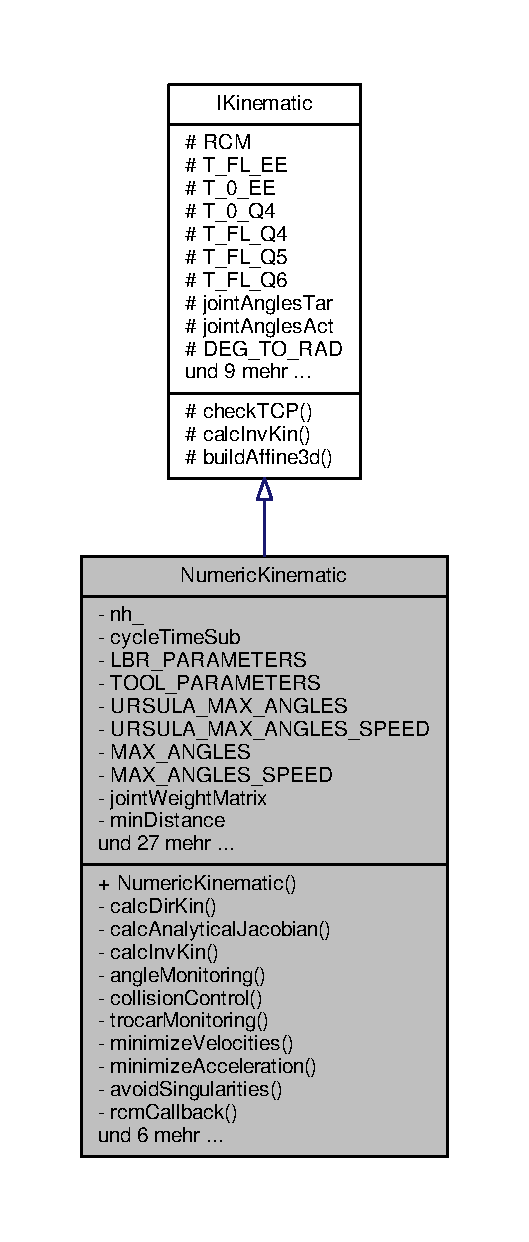
\includegraphics[height=550pt]{classNumericKinematic__inherit__graph}
\end{center}
\end{figure}


Zusammengehörigkeiten von Numeric\-Kinematic\-:
\nopagebreak
\begin{figure}[H]
\begin{center}
\leavevmode
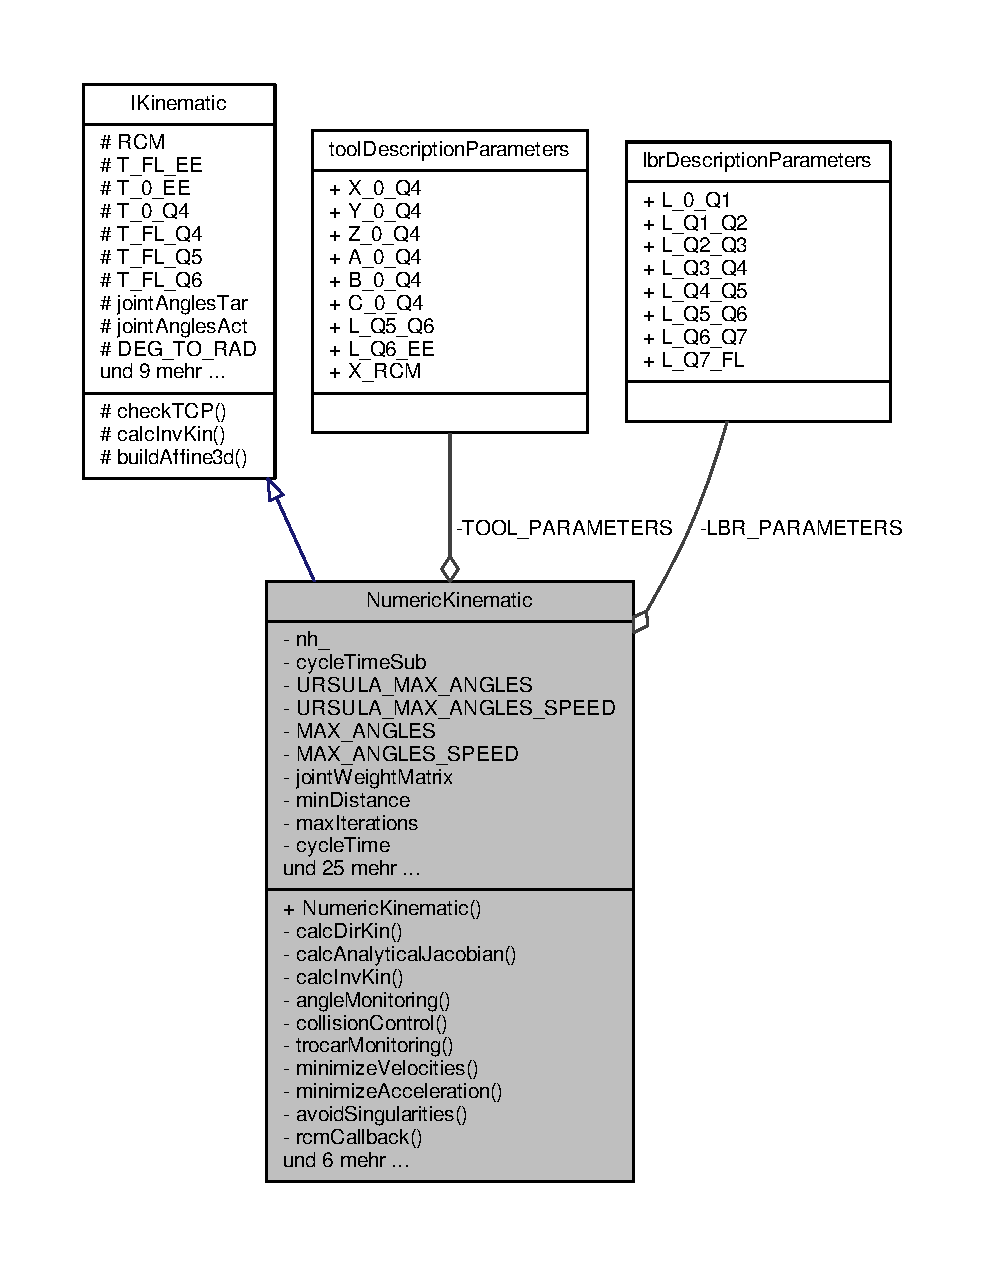
\includegraphics[width=350pt]{classNumericKinematic__coll__graph}
\end{center}
\end{figure}
\subsection*{Öffentliche Methoden}
\begin{DoxyCompactItemize}
\item 
\hypertarget{classNumericKinematic_aed713b319bef7e9bb52855d3b0c4b79c}{{\bfseries Numeric\-Kinematic} (ros\-::\-Node\-Handle \&)}\label{classNumericKinematic_aed713b319bef7e9bb52855d3b0c4b79c}

\end{DoxyCompactItemize}
\subsection*{Private Methoden}
\begin{DoxyCompactItemize}
\item 
Eigen\-::\-Vector\-Xd \hyperlink{classNumericKinematic_a48e3a4bce7cb5a0c410261cb110eb371}{calc\-Dir\-Kin} (Eigen\-::\-Vector\-Xd joint\-Angles)
\begin{DoxyCompactList}\small\item\em Berechnung der direkten Kinematik der Gesamtkinematik mit 10 Gelenkfreiheitsgraden. \end{DoxyCompactList}\item 
Eigen\-::\-Matrix\-Xd \hyperlink{classNumericKinematic_ac106c549b81876ea8310dd42e8530a56}{calc\-Analytical\-Jacobian} (Eigen\-::\-Vector\-Xd joint\-Angles)
\begin{DoxyCompactList}\small\item\em Berechnung der analytischen Jacobi-\/\-Matrix der Gesamtkinematik mit 10 Gelenkfreiheitsgraden. \end{DoxyCompactList}\item 
bool \hyperlink{classNumericKinematic_a39d3e132f2d0786815cc9b5dc94f186a}{calc\-Inv\-Kin} (Eigen\-::\-Affine3d \hyperlink{classIKinematic_a1c0a95317992b7fcaf26ab2bf9aaf3de}{T\-\_\-0\-\_\-\-E\-E})
\begin{DoxyCompactList}\small\item\em Berechnung der inversen Kinematik durch numerische Optimierung eines Least-\/\-Squares-\/\-Problem nach verschiedenen Kriterien. \end{DoxyCompactList}\item 
Eigen\-::\-Vector\-Xd \hyperlink{classNumericKinematic_ad3306dc5d1753c1bc403e5274c725ada}{angle\-Monitoring} (Eigen\-::\-Vector\-Xd delta\-Q, Eigen\-::\-Vector\-Xd q, double Hmax, double \&a)
\begin{DoxyCompactList}\small\item\em Überwacht die Einhaltung der maximalen Winkel und berechnet ein winkelabhängiges Potential. \end{DoxyCompactList}\item 
\hypertarget{classNumericKinematic_a7173a170876e1f2500feeb82b5f91b5e}{Eigen\-::\-Matrix\-Xd {\bfseries collision\-Control} (Eigen\-::\-Vector\-Xd q)}\label{classNumericKinematic_a7173a170876e1f2500feeb82b5f91b5e}

\item 
Eigen\-::\-Vector\-Xd \hyperlink{classNumericKinematic_ae480557185cc99b324bae2769afd9faf}{trocar\-Monitoring} (Eigen\-::\-Vector\-Xd q\-Act, Eigen\-::\-Vector\-Xd delta\-Q, Eigen\-::\-Matrix\-Xd \&A)
\begin{DoxyCompactList}\small\item\em Überwacht die Einhaltung des Trokarpunktes. \end{DoxyCompactList}\item 
Eigen\-::\-Matrix\-Xd \hyperlink{classNumericKinematic_a2b570a6bd42d5ff63923b3779810d38c}{minimize\-Velocities} (double \hyperlink{classNumericKinematic_aa96fd840d44735dcf5af2a6007cdd9a5}{cycle\-Time}, Eigen\-::\-Matrix\-Xd weight\-Matrix)
\begin{DoxyCompactList}\small\item\em Minimiert und verteilt die Gelenkwinkelgeschwindigkeiten abhängig von der Wichtungsmatrix. \end{DoxyCompactList}\item 
Eigen\-::\-Matrix\-Xd \hyperlink{classNumericKinematic_ad6a2a0fc7fee25d1a536bdca40aad47c}{minimize\-Acceleration} (double \hyperlink{classNumericKinematic_aa96fd840d44735dcf5af2a6007cdd9a5}{cycle\-Time}, Eigen\-::\-Matrix\-Xd weight\-Matrix, Eigen\-::\-Vector\-Xd delta\-Q, Eigen\-::\-Matrix\-Xd \&a)
\begin{DoxyCompactList}\small\item\em Minimiert und verteilt die Gelenkwinkelbeschleunigungen abhängig von der Wichtungsmatrix. \end{DoxyCompactList}\item 
Eigen\-::\-Vector\-Xd \hyperlink{classNumericKinematic_a6b467211611418e500d58d0d8d172698}{avoid\-Singularities} (Eigen\-::\-Vector\-Xd q\-Act, Eigen\-::\-Vector\-Xd q\-Offset, double weight, double \&a)
\begin{DoxyCompactList}\small\item\em Vermeidet Singularitäten durch ein Kosinusquadratpotential. \end{DoxyCompactList}\item 
\hypertarget{classNumericKinematic_a95a6dfcf5c773c0a8e46befe21f86d18}{bool {\bfseries rcm\-Callback} (masterslave\-::\-Numeric\-Kinematic\-R\-C\-M\-::\-Request \&, masterslave\-::\-Numeric\-Kinematic\-R\-C\-M\-::\-Response \&)}\label{classNumericKinematic_a95a6dfcf5c773c0a8e46befe21f86d18}

\item 
\hypertarget{classNumericKinematic_adc3915a8772203f9c39a31a8869c4206}{bool {\bfseries direct\-Kinematics\-Callback} (masterslave\-::\-Numeric\-Kinematic\-Direct\-Kinematics\-::\-Request \&, masterslave\-::\-Numeric\-Kinematic\-Direct\-Kinematics\-::\-Response \&)}\label{classNumericKinematic_adc3915a8772203f9c39a31a8869c4206}

\item 
\hypertarget{classNumericKinematic_a703b5b58b9edb0039f296e64f8b6e3ab}{bool {\bfseries inverse\-Kinematics\-Callback} (masterslave\-::\-Numeric\-Kinematic\-Inverse\-Kinematics\-::\-Request \&, masterslave\-::\-Numeric\-Kinematic\-Inverse\-Kinematics\-::\-Response \&)}\label{classNumericKinematic_a703b5b58b9edb0039f296e64f8b6e3ab}

\item 
\hypertarget{classNumericKinematic_a6d621216d4e3779465caf121ed931710}{void {\bfseries cycle\-Time\-Callback} (const std\-\_\-msgs\-::\-Float64\-Const\-Ptr \&)}\label{classNumericKinematic_a6d621216d4e3779465caf121ed931710}

\item 
\hypertarget{classNumericKinematic_a51d9888088eec181ecc3846006348ce7}{void {\bfseries configuration\-Callback} (masterslave\-::\-Numeric\-Kinematic\-Config \&config, uint32\-\_\-t level)}\label{classNumericKinematic_a51d9888088eec181ecc3846006348ce7}

\item 
Eigen\-::\-Vector\-Xd \hyperlink{classNumericKinematic_a4486d237a9ec27b6f092ffedf379e02c}{rotation2\-R\-P\-Y} (Eigen\-::\-Affine3d transformation)
\begin{DoxyCompactList}\small\item\em Umrechnung einer Rotation einer Affinen Transformation in Euler-\/\-Winkel und Übergabe der Translation. \end{DoxyCompactList}\item 
Eigen\-::\-Affine3d \hyperlink{classNumericKinematic_a6f116ab38ed9ff1aa0e90b710a4898f8}{build\-Affine3d} (const Eigen\-::\-Vector3d \&transl\-X\-Y\-Z, const Eigen\-::\-Vector3d \&axis\-Z\-Y\-X, bool zyx)
\begin{DoxyCompactList}\small\item\em Hilfsfunktion zur Erstellung von Affinen Transformationen aus einem Translationsvekt und den R\-P\-Y-\/\-Winkeln. \end{DoxyCompactList}\end{DoxyCompactItemize}
\subsection*{Private Attribute}
\begin{DoxyCompactItemize}
\item 
\hypertarget{classNumericKinematic_aa34a71fe4f46fe30dd97fc729bf9d41f}{ros\-::\-Node\-Handle {\bfseries nh\-\_\-}}\label{classNumericKinematic_aa34a71fe4f46fe30dd97fc729bf9d41f}

\item 
\hypertarget{classNumericKinematic_ad53a5e081b607e929b5dcd79ba597dfa}{ros\-::\-Subscriber {\bfseries cycle\-Time\-Sub}}\label{classNumericKinematic_ad53a5e081b607e929b5dcd79ba597dfa}

\item 
const \hyperlink{structlbrDescriptionParameters}{lbr\-Description\-Parameters} \hyperlink{classNumericKinematic_a1dc6a0780af1ef87cd5f6e8c95f1f7a7}{L\-B\-R\-\_\-\-P\-A\-R\-A\-M\-E\-T\-E\-R\-S} = \{ 0.\-160, 0.\-200, 0.\-200, 0.\-220, 0.\-180, 0.\-220, 0.\-076, 0.\-050\}
\begin{DoxyCompactList}\small\item\em Geometrische Parameter des L\-B\-R iiwa R820. \end{DoxyCompactList}\item 
const \hyperlink{structtoolDescriptionParameters}{tool\-Description\-Parameters} \hyperlink{classNumericKinematic_ae23ea272ef83d6d3285730fe33fa250b}{T\-O\-O\-L\-\_\-\-P\-A\-R\-A\-M\-E\-T\-E\-R\-S} = \{0.\-438, 0.\-0, 0.\-062, 0.\-0, 90.\-0, 0.\-0, 0.\-0088, 0.\-017, 0.\-305\}
\begin{DoxyCompactList}\small\item\em Geoemtrische Parameter des Werkzeuges. \end{DoxyCompactList}\item 
Eigen\-::\-Matrix$<$ double, 10, 1 $>$ \hyperlink{classNumericKinematic_a562cfd1d8c6b0f0074fb2796e8fbff13}{U\-R\-S\-U\-L\-A\-\_\-\-M\-A\-X\-\_\-\-A\-N\-G\-L\-E\-S}
\begin{DoxyCompactList}\small\item\em Vektor der maximalen Gelenkwinkel. \end{DoxyCompactList}\item 
Eigen\-::\-Matrix$<$ double, 10, 1 $>$ \hyperlink{classNumericKinematic_af6d15e97e215a9d8e552f1667bb6234f}{U\-R\-S\-U\-L\-A\-\_\-\-M\-A\-X\-\_\-\-A\-N\-G\-L\-E\-S\-\_\-\-S\-P\-E\-E\-D}
\begin{DoxyCompactList}\small\item\em Vektor der maximalen Gelenkwinkelgeschwindigkeiten. \end{DoxyCompactList}\item 
\hypertarget{classNumericKinematic_a146737bc121dfecf585f5dd1012c6fb1}{const double \hyperlink{classNumericKinematic_a146737bc121dfecf585f5dd1012c6fb1}{M\-A\-X\-\_\-\-A\-N\-G\-L\-E\-S} \mbox{[}10\mbox{]} = \{170$\ast$D\-E\-G\-\_\-\-T\-O\-\_\-\-R\-A\-D, 120$\ast$D\-E\-G\-\_\-\-T\-O\-\_\-\-R\-A\-D, 170$\ast$D\-E\-G\-\_\-\-T\-O\-\_\-\-R\-A\-D, 120$\ast$D\-E\-G\-\_\-\-T\-O\-\_\-\-R\-A\-D, 170$\ast$D\-E\-G\-\_\-\-T\-O\-\_\-\-R\-A\-D, 120$\ast$D\-E\-G\-\_\-\-T\-O\-\_\-\-R\-A\-D, 175$\ast$D\-E\-G\-\_\-\-T\-O\-\_\-\-R\-A\-D, 85$\ast$D\-E\-G\-\_\-\-T\-O\-\_\-\-R\-A\-D, 90$\ast$D\-E\-G\-\_\-\-T\-O\-\_\-\-R\-A\-D, 90$\ast$D\-E\-G\-\_\-\-T\-O\-\_\-\-R\-A\-D\}}\label{classNumericKinematic_a146737bc121dfecf585f5dd1012c6fb1}

\begin{DoxyCompactList}\small\item\em Array der maximalen Gelenkwinkel in \mbox{[}rad\mbox{]}. \end{DoxyCompactList}\item 
\hypertarget{classNumericKinematic_a2773f8d9aafe634b8f1e7f52142f98e8}{const double \hyperlink{classNumericKinematic_a2773f8d9aafe634b8f1e7f52142f98e8}{M\-A\-X\-\_\-\-A\-N\-G\-L\-E\-S\-\_\-\-S\-P\-E\-E\-D} \mbox{[}10\mbox{]} = \{ 85$\ast$D\-E\-G\-\_\-\-T\-O\-\_\-\-R\-A\-D, 85$\ast$D\-E\-G\-\_\-\-T\-O\-\_\-\-R\-A\-D, 100$\ast$D\-E\-G\-\_\-\-T\-O\-\_\-\-R\-A\-D, 75$\ast$D\-E\-G\-\_\-\-T\-O\-\_\-\-R\-A\-D, 130$\ast$D\-E\-G\-\_\-\-T\-O\-\_\-\-R\-A\-D, 135$\ast$D\-E\-G\-\_\-\-T\-O\-\_\-\-R\-A\-D, 135$\ast$D\-E\-G\-\_\-\-T\-O\-\_\-\-R\-A\-D, 135$\ast$D\-E\-G\-\_\-\-T\-O\-\_\-\-R\-A\-D, 135$\ast$D\-E\-G\-\_\-\-T\-O\-\_\-\-R\-A\-D, 135$\ast$D\-E\-G\-\_\-\-T\-O\-\_\-\-R\-A\-D\}}\label{classNumericKinematic_a2773f8d9aafe634b8f1e7f52142f98e8}

\begin{DoxyCompactList}\small\item\em Array der maximalen Gelenkwinkelgeschwindigkeiten in \mbox{[}rad/s\mbox{]}. \end{DoxyCompactList}\item 
\hypertarget{classNumericKinematic_af1e1bf1f56436abba6d1d6582449600b}{Eigen\-::\-Matrix$<$ double, 10, 10 $>$ \hyperlink{classNumericKinematic_af1e1bf1f56436abba6d1d6582449600b}{joint\-Weight\-Matrix}}\label{classNumericKinematic_af1e1bf1f56436abba6d1d6582449600b}

\begin{DoxyCompactList}\small\item\em Diagonale Gelenkwinkelwichtungsmatrix \mbox{[}10x10\mbox{]}. \end{DoxyCompactList}\item 
\hypertarget{classNumericKinematic_aab2518847c6ad6c4a6cd33746ff4aec2}{const double \hyperlink{classNumericKinematic_aab2518847c6ad6c4a6cd33746ff4aec2}{min\-Distance} \{0.\-05\}}\label{classNumericKinematic_aab2518847c6ad6c4a6cd33746ff4aec2}

\begin{DoxyCompactList}\small\item\em Distanz ab der die Kollisionserkennung startt. \end{DoxyCompactList}\item 
\hypertarget{classNumericKinematic_ac07694cf3b68d0392d9d5045af85d92f}{const int \hyperlink{classNumericKinematic_ac07694cf3b68d0392d9d5045af85d92f}{max\-Iterations} \{10\}}\label{classNumericKinematic_ac07694cf3b68d0392d9d5045af85d92f}

\begin{DoxyCompactList}\small\item\em Maximale Anzahl der Iterations. \end{DoxyCompactList}\item 
\hypertarget{classNumericKinematic_aa96fd840d44735dcf5af2a6007cdd9a5}{double \hyperlink{classNumericKinematic_aa96fd840d44735dcf5af2a6007cdd9a5}{cycle\-Time}}\label{classNumericKinematic_aa96fd840d44735dcf5af2a6007cdd9a5}

\begin{DoxyCompactList}\small\item\em Zykluszeit. \end{DoxyCompactList}\item 
\hypertarget{classNumericKinematic_a92de01f45510f0c7d5c1d8872740efb8}{Eigen\-::\-Matrix$<$ double, 6, 1 $>$ \hyperlink{classNumericKinematic_a92de01f45510f0c7d5c1d8872740efb8}{cur\-E\-E\-Position}}\label{classNumericKinematic_a92de01f45510f0c7d5c1d8872740efb8}

\begin{DoxyCompactList}\small\item\em Aktuelle Endeffektorlage im Weltkoordinatensystem. \end{DoxyCompactList}\item 
\hypertarget{classNumericKinematic_ab77311c858600ae931ce1e34d95a1d6b}{Eigen\-::\-Matrix$<$ double, 6, 1 $>$ \hyperlink{classNumericKinematic_ab77311c858600ae931ce1e34d95a1d6b}{des\-E\-E\-Position}}\label{classNumericKinematic_ab77311c858600ae931ce1e34d95a1d6b}

\begin{DoxyCompactList}\small\item\em Gewünschte Endeffektorlage im Weltkoordinatensystem. \end{DoxyCompactList}\item 
Eigen\-::\-Affine3d \hyperlink{classNumericKinematic_a2b3815e7cce36ab203257bf8f5e2e236}{T\-\_\-0\-\_\-\-Q1}
\begin{DoxyCompactList}\small\item\em Lage des Gelenks Q1 im Weltkoordinatensystem. \end{DoxyCompactList}\item 
\hypertarget{classNumericKinematic_aa77f38a33ab7d209446df174a9ba61dc}{Eigen\-::\-Affine3d \hyperlink{classNumericKinematic_aa77f38a33ab7d209446df174a9ba61dc}{T\-\_\-0\-\_\-\-Q2}}\label{classNumericKinematic_aa77f38a33ab7d209446df174a9ba61dc}

\begin{DoxyCompactList}\small\item\em Lage des Gelenks Q2 im Weltkoordinatensystem. \end{DoxyCompactList}\item 
\hypertarget{classNumericKinematic_a847dcb3a66622d8e67e9676e881e5030}{Eigen\-::\-Affine3d \hyperlink{classNumericKinematic_a847dcb3a66622d8e67e9676e881e5030}{T\-\_\-0\-\_\-\-Q3}}\label{classNumericKinematic_a847dcb3a66622d8e67e9676e881e5030}

\begin{DoxyCompactList}\small\item\em Lage des Gelenks Q3 im Weltkoordinatensystem. \end{DoxyCompactList}\item 
\hypertarget{classNumericKinematic_a2dfc754d67f7c27cce1d05fd3d26fcbb}{Eigen\-::\-Affine3d \hyperlink{classNumericKinematic_a2dfc754d67f7c27cce1d05fd3d26fcbb}{T\-\_\-0\-\_\-\-Q4}}\label{classNumericKinematic_a2dfc754d67f7c27cce1d05fd3d26fcbb}

\begin{DoxyCompactList}\small\item\em Lage des Gelenks Q4 im Weltkoordinatensystem. \end{DoxyCompactList}\item 
\hypertarget{classNumericKinematic_a72426b1ae1945e5a09daafb69e2d1deb}{Eigen\-::\-Affine3d \hyperlink{classNumericKinematic_a72426b1ae1945e5a09daafb69e2d1deb}{T\-\_\-0\-\_\-\-Q5}}\label{classNumericKinematic_a72426b1ae1945e5a09daafb69e2d1deb}

\begin{DoxyCompactList}\small\item\em Lage des Gelenks Q5 im Weltkoordinatensystem. \end{DoxyCompactList}\item 
\hypertarget{classNumericKinematic_ad79c09069f78450e9a6c3657a390f4c2}{Eigen\-::\-Affine3d \hyperlink{classNumericKinematic_ad79c09069f78450e9a6c3657a390f4c2}{T\-\_\-0\-\_\-\-Q6}}\label{classNumericKinematic_ad79c09069f78450e9a6c3657a390f4c2}

\begin{DoxyCompactList}\small\item\em Lage des Gelenks Q6 im Weltkoordinatensystem. \end{DoxyCompactList}\item 
\hypertarget{classNumericKinematic_a5a64e4e800ee0ae6da0b2df4b2fe35cf}{Eigen\-::\-Affine3d \hyperlink{classNumericKinematic_a5a64e4e800ee0ae6da0b2df4b2fe35cf}{T\-\_\-0\-\_\-\-Q7}}\label{classNumericKinematic_a5a64e4e800ee0ae6da0b2df4b2fe35cf}

\begin{DoxyCompactList}\small\item\em Lage des Gelenks Q7 im Weltkoordinatensystem. \end{DoxyCompactList}\item 
\hypertarget{classNumericKinematic_a1d4687858b97b4df67401ddb3bd2c5b4}{Eigen\-::\-Affine3d \hyperlink{classNumericKinematic_a1d4687858b97b4df67401ddb3bd2c5b4}{T\-\_\-0\-\_\-\-F\-L}}\label{classNumericKinematic_a1d4687858b97b4df67401ddb3bd2c5b4}

\begin{DoxyCompactList}\small\item\em Lage des Roboterflanschs im Weltkoordinatensystem. \end{DoxyCompactList}\item 
\hypertarget{classNumericKinematic_a8e6f0493f1fc31b3c4e33b04ace1c6cc}{Eigen\-::\-Affine3d {\bfseries T\-\_\-0\-\_\-\-S\-C\-H}}\label{classNumericKinematic_a8e6f0493f1fc31b3c4e33b04ace1c6cc}

\item 
\hypertarget{classNumericKinematic_a11368a132121a5dc639003ceeca8d0ec}{Eigen\-::\-Affine3d \hyperlink{classNumericKinematic_a11368a132121a5dc639003ceeca8d0ec}{T\-\_\-0\-\_\-\-Q8}}\label{classNumericKinematic_a11368a132121a5dc639003ceeca8d0ec}

\begin{DoxyCompactList}\small\item\em Lage des Gelenks Q8 im Weltkoordinatensystem. \end{DoxyCompactList}\item 
\hypertarget{classNumericKinematic_a581d613f2ff4e2f8abf05690eb7eb08a}{Eigen\-::\-Affine3d \hyperlink{classNumericKinematic_a581d613f2ff4e2f8abf05690eb7eb08a}{T\-\_\-0\-\_\-\-Q9}}\label{classNumericKinematic_a581d613f2ff4e2f8abf05690eb7eb08a}

\begin{DoxyCompactList}\small\item\em Lage des Gelenks Q9 im Weltkoordinatensystem. \end{DoxyCompactList}\item 
\hypertarget{classNumericKinematic_a628bae48695ed11d4e6072889e75062b}{Eigen\-::\-Affine3d \hyperlink{classNumericKinematic_a628bae48695ed11d4e6072889e75062b}{T\-\_\-0\-\_\-\-Q10}}\label{classNumericKinematic_a628bae48695ed11d4e6072889e75062b}

\begin{DoxyCompactList}\small\item\em Lage des Gelenks Q10 im Weltkoordinatensystem. \end{DoxyCompactList}\item 
double \hyperlink{classNumericKinematic_a2e5991d67d0e27b171a1ef8f4b759913}{collision\-Avoidance\-Gain} \{0.\-0000001\}
\item 
double \hyperlink{classNumericKinematic_abcb83da2f2e4934765c8522ac0569405}{angle\-Monitoring\-Gain} \{0.\-0000001\}
\item 
double \hyperlink{classNumericKinematic_ab64580c565b5ddcadb7de6fc6d5bd766}{singularity\-Gain} \{0.\-000001\}
\item 
double \hyperlink{classNumericKinematic_a3f76ee7066ac853557b44fb1b46689cb}{acceleration\-Gain} \{0.\-0000001\}
\item 
double \hyperlink{classNumericKinematic_a3c0bd5b51e9bf070bd2570928feb1cc6}{velocity\-Gain} \{0.\-0000001\}
\item 
\hypertarget{classNumericKinematic_a668ce168ed4a3e917f95304153755788}{double \hyperlink{classNumericKinematic_a668ce168ed4a3e917f95304153755788}{max\-Speed} \{0.\-7\}}\label{classNumericKinematic_a668ce168ed4a3e917f95304153755788}

\begin{DoxyCompactList}\small\item\em max\-Speed decimal \end{DoxyCompactList}\item 
double \hyperlink{classNumericKinematic_a6691d8d0fa2579cc4408acec0d2e864b}{rescue\-Factor} \{0\}
\item 
\hypertarget{classNumericKinematic_a90d84f5207c4c6a956022ba26e3212ad}{double \hyperlink{classNumericKinematic_a90d84f5207c4c6a956022ba26e3212ad}{trocar\-Gain} \{1\}}\label{classNumericKinematic_a90d84f5207c4c6a956022ba26e3212ad}

\begin{DoxyCompactList}\small\item\em Gewichtung Einhaltung des Trokarpunktes. \end{DoxyCompactList}\item 
\hypertarget{classNumericKinematic_a3ca1ed22eb6d87ca796366015e1709d4}{double \hyperlink{classNumericKinematic_a3ca1ed22eb6d87ca796366015e1709d4}{tcp\-Gain} \{1\}}\label{classNumericKinematic_a3ca1ed22eb6d87ca796366015e1709d4}

\begin{DoxyCompactList}\small\item\em Gewichtung Einhaltung des T\-C\-P. \end{DoxyCompactList}\item 
Eigen\-::\-Matrix\-Xd \hyperlink{classNumericKinematic_a3d773d5b89a38a88ed664896fb139f48}{geom\-Jacobian}
\begin{DoxyCompactList}\small\item\em geometrische Jacobi-\/\-Matrix \end{DoxyCompactList}\item 
Eigen\-::\-Matrix\-Xd \hyperlink{classNumericKinematic_ae3fd64a575333037133ede9f2a412f76}{analytical\-Jacobian}
\begin{DoxyCompactList}\small\item\em analytische Jacobi-\/\-Matrix \end{DoxyCompactList}\end{DoxyCompactItemize}
\subsection*{Weitere Geerbte Elemente}


\subsection{Ausführliche Beschreibung}
Klasse zur Berechnung der Kinematiken des Gesamtsystems mit 10 Achsen. Die inverse Kinematik wird numerisch mittels eines Least-\/\-Square-\/\-Problems gelöst Die Klasse berechnet die direkte und inverse Kinematik eines Gesamtsystems bestehend aus L\-B\-R iiwa und dem Laparoskop. Es besitzt insgesamt 10 Achsen, da der Trokarpunkt eingehalten werden muss, bleibt noch eine Redundanz mit Dimension 2 zur Optimierung der Gelenkwinkelkonfiguration. Diese können mit verschiedenen Optimierungskriterien, wie Singularitätsvermeidung, Kollisionsvermeidung, Geschwindigkeits-\/ und Beschleunigungsminimierung, sowie einer Winkelwächterfunktion parametriert werden Zum Lösen wird der Algorithmus aus Quad\-Prog++ eingesetzt, der auf die Eigen-\/\-Bibliothek umgeschrieben wurde. 

\begin{DoxySeeAlso}{Siehe auch}
\hyperlink{eiquadprog_8hpp_source}{eiquadprog.\-hpp}
\end{DoxySeeAlso}
\begin{DoxyAuthor}{Autor}
Fabian Baier 
\end{DoxyAuthor}
\begin{DoxyDate}{Datum}
20.\-03.\-2016 
\end{DoxyDate}
\begin{DoxySeeAlso}{Siehe auch}
\hyperlink{classIKinematic}{I\-Kinematic} 
\end{DoxySeeAlso}


\subsection{Dokumentation der Elementfunktionen}
\hypertarget{classNumericKinematic_ad3306dc5d1753c1bc403e5274c725ada}{\index{Numeric\-Kinematic@{Numeric\-Kinematic}!angle\-Monitoring@{angle\-Monitoring}}
\index{angle\-Monitoring@{angle\-Monitoring}!NumericKinematic@{Numeric\-Kinematic}}
\subsubsection[{angle\-Monitoring}]{\setlength{\rightskip}{0pt plus 5cm}Numeric\-Kinematic\-::angle\-Monitoring (
\begin{DoxyParamCaption}
\item[{Eigen\-::\-Vector\-Xd}]{delta\-Q, }
\item[{Eigen\-::\-Vector\-Xd}]{q, }
\item[{double}]{Hmax, }
\item[{double \&}]{a}
\end{DoxyParamCaption}
)\hspace{0.3cm}{\ttfamily [private]}}}\label{classNumericKinematic_ad3306dc5d1753c1bc403e5274c725ada}


Überwacht die Einhaltung der maximalen Winkel und berechnet ein winkelabhängiges Potential. 


\begin{DoxyParams}{Parameter}
{\em delta\-Q} & Winkeldifferenz zwischen dem vorherigen Iterationsschritt und dem in dem vorherigen Durchlauf bestimmten Gelenkwinkelvektor \\
\hline
{\em q} & Aktueller Gelenkwinkelvektor der vorherigen Iteration \\
\hline
{\em Hmax} & Maximales Potential der Potentialfunktion \\
\hline
{\em a} & Referenz auf das berechnete Potential \\
\hline
\end{DoxyParams}
\begin{DoxyReturn}{Rückgabe}
Ableitung des Potentials nach den Gelenkwinkeln 
\end{DoxyReturn}
\hypertarget{classNumericKinematic_a6b467211611418e500d58d0d8d172698}{\index{Numeric\-Kinematic@{Numeric\-Kinematic}!avoid\-Singularities@{avoid\-Singularities}}
\index{avoid\-Singularities@{avoid\-Singularities}!NumericKinematic@{Numeric\-Kinematic}}
\subsubsection[{avoid\-Singularities}]{\setlength{\rightskip}{0pt plus 5cm}Numeric\-Kinematic\-::avoid\-Singularities (
\begin{DoxyParamCaption}
\item[{Eigen\-::\-Vector\-Xd}]{q\-Act, }
\item[{Eigen\-::\-Vector\-Xd}]{q\-Offset, }
\item[{double}]{weight, }
\item[{double \&}]{a}
\end{DoxyParamCaption}
)\hspace{0.3cm}{\ttfamily [private]}}}\label{classNumericKinematic_a6b467211611418e500d58d0d8d172698}


Vermeidet Singularitäten durch ein Kosinusquadratpotential. 


\begin{DoxyParams}{Parameter}
{\em q\-Act} & Aktueller Gelenkwinkelvektor \\
\hline
{\em q\-Offset} & Verschiebung des Kosinusterms \\
\hline
{\em weight} & Maximales Potential \\
\hline
{\em a} & Referenz auf das Potential \\
\hline
\end{DoxyParams}
\begin{DoxyReturn}{Rückgabe}
Vektor der Gelenkwinkelpotentiale abgeleitet nach den Gelenkwinkeln 
\end{DoxyReturn}
\hypertarget{classNumericKinematic_a6f116ab38ed9ff1aa0e90b710a4898f8}{\index{Numeric\-Kinematic@{Numeric\-Kinematic}!build\-Affine3d@{build\-Affine3d}}
\index{build\-Affine3d@{build\-Affine3d}!NumericKinematic@{Numeric\-Kinematic}}
\subsubsection[{build\-Affine3d}]{\setlength{\rightskip}{0pt plus 5cm}Numeric\-Kinematic\-::build\-Affine3d (
\begin{DoxyParamCaption}
\item[{const Eigen\-::\-Vector3d \&}]{transl\-X\-Y\-Z, }
\item[{const Eigen\-::\-Vector3d \&}]{axis\-Z\-Y\-X, }
\item[{bool}]{zyx}
\end{DoxyParamCaption}
)\hspace{0.3cm}{\ttfamily [private]}}}\label{classNumericKinematic_a6f116ab38ed9ff1aa0e90b710a4898f8}


Hilfsfunktion zur Erstellung von Affinen Transformationen aus einem Translationsvekt und den R\-P\-Y-\/\-Winkeln. 


\begin{DoxyParams}{Parameter}
{\em transl\-X\-Y\-Z} & Translationsvektor \\
\hline
{\em axis\-Z\-Y\-X} & Rotationsvektor \\
\hline
{\em zyx} & Flag zur Festlegung der Rotationsrichtung \\
\hline
\end{DoxyParams}
\begin{DoxyReturn}{Rückgabe}
Affine Transformation 
\end{DoxyReturn}
\begin{DoxySeeAlso}{Siehe auch}
\hyperlink{classIKinematic}{I\-Kinematic} 
\end{DoxySeeAlso}
\hypertarget{classNumericKinematic_ac106c549b81876ea8310dd42e8530a56}{\index{Numeric\-Kinematic@{Numeric\-Kinematic}!calc\-Analytical\-Jacobian@{calc\-Analytical\-Jacobian}}
\index{calc\-Analytical\-Jacobian@{calc\-Analytical\-Jacobian}!NumericKinematic@{Numeric\-Kinematic}}
\subsubsection[{calc\-Analytical\-Jacobian}]{\setlength{\rightskip}{0pt plus 5cm}Numeric\-Kinematic\-::calc\-Analytical\-Jacobian (
\begin{DoxyParamCaption}
\item[{Eigen\-::\-Vector\-Xd}]{joint\-Angles}
\end{DoxyParamCaption}
)\hspace{0.3cm}{\ttfamily [private]}}}\label{classNumericKinematic_ac106c549b81876ea8310dd42e8530a56}


Berechnung der analytischen Jacobi-\/\-Matrix der Gesamtkinematik mit 10 Gelenkfreiheitsgraden. 


\begin{DoxyParams}{Parameter}
{\em joint\-Angles} & Gelenkwinkelvektor \\
\hline
\end{DoxyParams}
\begin{DoxyReturn}{Rückgabe}
Analytische Jacobi-\/\-Matrix mit dem rotatorischen Anteil in Bezug auf Eulerwinkel 
\end{DoxyReturn}
\hypertarget{classNumericKinematic_a48e3a4bce7cb5a0c410261cb110eb371}{\index{Numeric\-Kinematic@{Numeric\-Kinematic}!calc\-Dir\-Kin@{calc\-Dir\-Kin}}
\index{calc\-Dir\-Kin@{calc\-Dir\-Kin}!NumericKinematic@{Numeric\-Kinematic}}
\subsubsection[{calc\-Dir\-Kin}]{\setlength{\rightskip}{0pt plus 5cm}Numeric\-Kinematic\-::calc\-Dir\-Kin (
\begin{DoxyParamCaption}
\item[{Eigen\-::\-Vector\-Xd}]{joint\-Angles}
\end{DoxyParamCaption}
)\hspace{0.3cm}{\ttfamily [private]}}}\label{classNumericKinematic_a48e3a4bce7cb5a0c410261cb110eb371}


Berechnung der direkten Kinematik der Gesamtkinematik mit 10 Gelenkfreiheitsgraden. 


\begin{DoxyParams}{Parameter}
{\em joint\-Angles} & Gelenkwinkelvektor \\
\hline
\end{DoxyParams}
\begin{DoxyReturn}{Rückgabe}
Kartesische Position und Vektor der Eulerwinkel in Z-\/\-Y'-\/\-X''-\/\-Reihenfolge 
\end{DoxyReturn}
\hypertarget{classNumericKinematic_a39d3e132f2d0786815cc9b5dc94f186a}{\index{Numeric\-Kinematic@{Numeric\-Kinematic}!calc\-Inv\-Kin@{calc\-Inv\-Kin}}
\index{calc\-Inv\-Kin@{calc\-Inv\-Kin}!NumericKinematic@{Numeric\-Kinematic}}
\subsubsection[{calc\-Inv\-Kin}]{\setlength{\rightskip}{0pt plus 5cm}Numeric\-Kinematic\-::calc\-Inv\-Kin (
\begin{DoxyParamCaption}
\item[{Eigen\-::\-Affine3d}]{T\-\_\-0\-\_\-\-E\-E}
\end{DoxyParamCaption}
)\hspace{0.3cm}{\ttfamily [private]}, {\ttfamily [virtual]}}}\label{classNumericKinematic_a39d3e132f2d0786815cc9b5dc94f186a}


Berechnung der inversen Kinematik durch numerische Optimierung eines Least-\/\-Squares-\/\-Problem nach verschiedenen Kriterien. 


\begin{DoxyParams}{Parameter}
{\em T\-\_\-0\-\_\-\-E\-E} & gewünschte T\-C\-P-\/\-Lage \\
\hline
\end{DoxyParams}
\begin{DoxyReturn}{Rückgabe}
Flag, ob der definierte Arbeitsraum eingehalten wurde 
\end{DoxyReturn}


Implementiert \hyperlink{classIKinematic_a6f95d80c4330253643c49a758404e4a7}{I\-Kinematic}.

\hypertarget{classNumericKinematic_ad6a2a0fc7fee25d1a536bdca40aad47c}{\index{Numeric\-Kinematic@{Numeric\-Kinematic}!minimize\-Acceleration@{minimize\-Acceleration}}
\index{minimize\-Acceleration@{minimize\-Acceleration}!NumericKinematic@{Numeric\-Kinematic}}
\subsubsection[{minimize\-Acceleration}]{\setlength{\rightskip}{0pt plus 5cm}Numeric\-Kinematic\-::minimize\-Acceleration (
\begin{DoxyParamCaption}
\item[{double}]{cycle\-Time, }
\item[{Eigen\-::\-Matrix\-Xd}]{weight\-Matrix, }
\item[{Eigen\-::\-Vector\-Xd}]{delta\-Q, }
\item[{Eigen\-::\-Matrix\-Xd \&}]{a}
\end{DoxyParamCaption}
)\hspace{0.3cm}{\ttfamily [private]}}}\label{classNumericKinematic_ad6a2a0fc7fee25d1a536bdca40aad47c}


Minimiert und verteilt die Gelenkwinkelbeschleunigungen abhängig von der Wichtungsmatrix. 


\begin{DoxyParams}{Parameter}
{\em cycle\-Time} & Zykluszeit \\
\hline
{\em weight\-Matrix} & Wichtungsmatrix \\
\hline
{\em delta\-Q} & Winkeldifferenz zwischen dem vorherigen Iterationsschritt und dem in dem vorherigen Durchlauf bestimmten Gelenkwinkelvektor \\
\hline
{\em a} & Referenz auf das Potential \\
\hline
\end{DoxyParams}
\begin{DoxyReturn}{Rückgabe}
Vektor der Gelenkwinkelpotentiale abgeleitet nach den Gelenkwinkeln 
\end{DoxyReturn}
\hypertarget{classNumericKinematic_a2b570a6bd42d5ff63923b3779810d38c}{\index{Numeric\-Kinematic@{Numeric\-Kinematic}!minimize\-Velocities@{minimize\-Velocities}}
\index{minimize\-Velocities@{minimize\-Velocities}!NumericKinematic@{Numeric\-Kinematic}}
\subsubsection[{minimize\-Velocities}]{\setlength{\rightskip}{0pt plus 5cm}Numeric\-Kinematic\-::minimize\-Velocities (
\begin{DoxyParamCaption}
\item[{double}]{cycle\-Time, }
\item[{Eigen\-::\-Matrix\-Xd}]{weight\-Matrix}
\end{DoxyParamCaption}
)\hspace{0.3cm}{\ttfamily [private]}}}\label{classNumericKinematic_a2b570a6bd42d5ff63923b3779810d38c}


Minimiert und verteilt die Gelenkwinkelgeschwindigkeiten abhängig von der Wichtungsmatrix. 


\begin{DoxyParams}{Parameter}
{\em cycle\-Time} & Zykluszeit \\
\hline
{\em weight\-Matrix} & Wichtungsmatrix \\
\hline
\end{DoxyParams}
\begin{DoxyReturn}{Rückgabe}
Vektor der Gelenkwinkelpotentiale abgeleitet nach den Gelenkwinkeln 
\end{DoxyReturn}
\hypertarget{classNumericKinematic_a4486d237a9ec27b6f092ffedf379e02c}{\index{Numeric\-Kinematic@{Numeric\-Kinematic}!rotation2\-R\-P\-Y@{rotation2\-R\-P\-Y}}
\index{rotation2\-R\-P\-Y@{rotation2\-R\-P\-Y}!NumericKinematic@{Numeric\-Kinematic}}
\subsubsection[{rotation2\-R\-P\-Y}]{\setlength{\rightskip}{0pt plus 5cm}Numeric\-Kinematic\-::rotation2\-R\-P\-Y (
\begin{DoxyParamCaption}
\item[{Eigen\-::\-Affine3d}]{transformation}
\end{DoxyParamCaption}
)\hspace{0.3cm}{\ttfamily [private]}}}\label{classNumericKinematic_a4486d237a9ec27b6f092ffedf379e02c}


Umrechnung einer Rotation einer Affinen Transformation in Euler-\/\-Winkel und Übergabe der Translation. 


\begin{DoxyParams}{Parameter}
{\em transformation} & Transformation \\
\hline
\end{DoxyParams}
\begin{DoxyReturn}{Rückgabe}
Vektor mit Translation und Rotation in Euler-\/\-Winkeln 
\end{DoxyReturn}
\hypertarget{classNumericKinematic_ae480557185cc99b324bae2769afd9faf}{\index{Numeric\-Kinematic@{Numeric\-Kinematic}!trocar\-Monitoring@{trocar\-Monitoring}}
\index{trocar\-Monitoring@{trocar\-Monitoring}!NumericKinematic@{Numeric\-Kinematic}}
\subsubsection[{trocar\-Monitoring}]{\setlength{\rightskip}{0pt plus 5cm}Numeric\-Kinematic\-::trocar\-Monitoring (
\begin{DoxyParamCaption}
\item[{Eigen\-::\-Vector\-Xd}]{q\-Act, }
\item[{Eigen\-::\-Vector\-Xd}]{delta\-Q, }
\item[{Eigen\-::\-Matrix\-Xd \&}]{A}
\end{DoxyParamCaption}
)\hspace{0.3cm}{\ttfamily [private]}}}\label{classNumericKinematic_ae480557185cc99b324bae2769afd9faf}


Überwacht die Einhaltung des Trokarpunktes. 


\begin{DoxyParams}{Parameter}
{\em q\-Act} & Aktueller Gelenkwinkelvektor der vorherigen Iteration \\
\hline
{\em delta\-Q} & Winkeldifferenz zwischen dem vorherigen Iterationsschritt und dem in dem vorherigen Durchlauf bestimmten Gelenkwinkelvektor \\
\hline
{\em A} & Jacobi-\/\-Matrix der Potentialfunktion \\
\hline
\end{DoxyParams}
\begin{DoxyReturn}{Rückgabe}
Vektor der freiheitsgradabhängigen Potentiale 
\end{DoxyReturn}


\subsection{Dokumentation der Datenelemente}
\hypertarget{classNumericKinematic_a3f76ee7066ac853557b44fb1b46689cb}{\index{Numeric\-Kinematic@{Numeric\-Kinematic}!acceleration\-Gain@{acceleration\-Gain}}
\index{acceleration\-Gain@{acceleration\-Gain}!NumericKinematic@{Numeric\-Kinematic}}
\subsubsection[{acceleration\-Gain}]{\setlength{\rightskip}{0pt plus 5cm}Numeric\-Kinematic\-::acceleration\-Gain \{0.\-0000001\}\hspace{0.3cm}{\ttfamily [private]}}}\label{classNumericKinematic_a3f76ee7066ac853557b44fb1b46689cb}
\begin{DoxySeeAlso}{Siehe auch}
acceleration\-Minimization 
\end{DoxySeeAlso}
\hypertarget{classNumericKinematic_ae3fd64a575333037133ede9f2a412f76}{\index{Numeric\-Kinematic@{Numeric\-Kinematic}!analytical\-Jacobian@{analytical\-Jacobian}}
\index{analytical\-Jacobian@{analytical\-Jacobian}!NumericKinematic@{Numeric\-Kinematic}}
\subsubsection[{analytical\-Jacobian}]{\setlength{\rightskip}{0pt plus 5cm}Numeric\-Kinematic\-::analytical\-Jacobian\hspace{0.3cm}{\ttfamily [private]}}}\label{classNumericKinematic_ae3fd64a575333037133ede9f2a412f76}


analytische Jacobi-\/\-Matrix 

\begin{DoxySeeAlso}{Siehe auch}
calculate\-Analytical\-Jacobian 
\end{DoxySeeAlso}
\hypertarget{classNumericKinematic_abcb83da2f2e4934765c8522ac0569405}{\index{Numeric\-Kinematic@{Numeric\-Kinematic}!angle\-Monitoring\-Gain@{angle\-Monitoring\-Gain}}
\index{angle\-Monitoring\-Gain@{angle\-Monitoring\-Gain}!NumericKinematic@{Numeric\-Kinematic}}
\subsubsection[{angle\-Monitoring\-Gain}]{\setlength{\rightskip}{0pt plus 5cm}Numeric\-Kinematic\-::angle\-Monitoring\-Gain \{0.\-0000001\}\hspace{0.3cm}{\ttfamily [private]}}}\label{classNumericKinematic_abcb83da2f2e4934765c8522ac0569405}
\begin{DoxySeeAlso}{Siehe auch}
\hyperlink{classNumericKinematic_ad3306dc5d1753c1bc403e5274c725ada}{angle\-Monitoring} 
\end{DoxySeeAlso}
\hypertarget{classNumericKinematic_a2e5991d67d0e27b171a1ef8f4b759913}{\index{Numeric\-Kinematic@{Numeric\-Kinematic}!collision\-Avoidance\-Gain@{collision\-Avoidance\-Gain}}
\index{collision\-Avoidance\-Gain@{collision\-Avoidance\-Gain}!NumericKinematic@{Numeric\-Kinematic}}
\subsubsection[{collision\-Avoidance\-Gain}]{\setlength{\rightskip}{0pt plus 5cm}Numeric\-Kinematic\-::collision\-Avoidance\-Gain \{0.\-0000001\}\hspace{0.3cm}{\ttfamily [private]}}}\label{classNumericKinematic_a2e5991d67d0e27b171a1ef8f4b759913}
\begin{DoxySeeAlso}{Siehe auch}
collision\-Avoidance 
\end{DoxySeeAlso}
\hypertarget{classNumericKinematic_a3d773d5b89a38a88ed664896fb139f48}{\index{Numeric\-Kinematic@{Numeric\-Kinematic}!geom\-Jacobian@{geom\-Jacobian}}
\index{geom\-Jacobian@{geom\-Jacobian}!NumericKinematic@{Numeric\-Kinematic}}
\subsubsection[{geom\-Jacobian}]{\setlength{\rightskip}{0pt plus 5cm}Numeric\-Kinematic\-::geom\-Jacobian\hspace{0.3cm}{\ttfamily [private]}}}\label{classNumericKinematic_a3d773d5b89a38a88ed664896fb139f48}


geometrische Jacobi-\/\-Matrix 

\begin{DoxySeeAlso}{Siehe auch}
calculate\-Analytical\-Jacobian 
\end{DoxySeeAlso}
\hypertarget{classNumericKinematic_a1dc6a0780af1ef87cd5f6e8c95f1f7a7}{\index{Numeric\-Kinematic@{Numeric\-Kinematic}!L\-B\-R\-\_\-\-P\-A\-R\-A\-M\-E\-T\-E\-R\-S@{L\-B\-R\-\_\-\-P\-A\-R\-A\-M\-E\-T\-E\-R\-S}}
\index{L\-B\-R\-\_\-\-P\-A\-R\-A\-M\-E\-T\-E\-R\-S@{L\-B\-R\-\_\-\-P\-A\-R\-A\-M\-E\-T\-E\-R\-S}!NumericKinematic@{Numeric\-Kinematic}}
\subsubsection[{L\-B\-R\-\_\-\-P\-A\-R\-A\-M\-E\-T\-E\-R\-S}]{\setlength{\rightskip}{0pt plus 5cm}Numeric\-Kinematic\-::\-L\-B\-R\-\_\-\-P\-A\-R\-A\-M\-E\-T\-E\-R\-S = \{ 0.\-160, 0.\-200, 0.\-200, 0.\-220, 0.\-180, 0.\-220, 0.\-076, 0.\-050\}\hspace{0.3cm}{\ttfamily [private]}}}\label{classNumericKinematic_a1dc6a0780af1ef87cd5f6e8c95f1f7a7}


Geometrische Parameter des L\-B\-R iiwa R820. 

\begin{DoxySeeAlso}{Siehe auch}
\hyperlink{DescriptionParameters_8h_source}{Description\-Parameters.\-h} 
\end{DoxySeeAlso}
\hypertarget{classNumericKinematic_a6691d8d0fa2579cc4408acec0d2e864b}{\index{Numeric\-Kinematic@{Numeric\-Kinematic}!rescue\-Factor@{rescue\-Factor}}
\index{rescue\-Factor@{rescue\-Factor}!NumericKinematic@{Numeric\-Kinematic}}
\subsubsection[{rescue\-Factor}]{\setlength{\rightskip}{0pt plus 5cm}Numeric\-Kinematic\-::rescue\-Factor \{0\}\hspace{0.3cm}{\ttfamily [private]}}}\label{classNumericKinematic_a6691d8d0fa2579cc4408acec0d2e864b}
\begin{DoxyRefDesc}{Veraltet}
\item[\hyperlink{deprecated__deprecated000005}{Veraltet}]\end{DoxyRefDesc}
\hypertarget{classNumericKinematic_ab64580c565b5ddcadb7de6fc6d5bd766}{\index{Numeric\-Kinematic@{Numeric\-Kinematic}!singularity\-Gain@{singularity\-Gain}}
\index{singularity\-Gain@{singularity\-Gain}!NumericKinematic@{Numeric\-Kinematic}}
\subsubsection[{singularity\-Gain}]{\setlength{\rightskip}{0pt plus 5cm}Numeric\-Kinematic\-::singularity\-Gain \{0.\-000001\}\hspace{0.3cm}{\ttfamily [private]}}}\label{classNumericKinematic_ab64580c565b5ddcadb7de6fc6d5bd766}
\begin{DoxySeeAlso}{Siehe auch}
singularity\-Avoidance 
\end{DoxySeeAlso}
\hypertarget{classNumericKinematic_a2b3815e7cce36ab203257bf8f5e2e236}{\index{Numeric\-Kinematic@{Numeric\-Kinematic}!T\-\_\-0\-\_\-\-Q1@{T\-\_\-0\-\_\-\-Q1}}
\index{T\-\_\-0\-\_\-\-Q1@{T\-\_\-0\-\_\-\-Q1}!NumericKinematic@{Numeric\-Kinematic}}
\subsubsection[{T\-\_\-0\-\_\-\-Q1}]{\setlength{\rightskip}{0pt plus 5cm}Numeric\-Kinematic\-::\-T\-\_\-0\-\_\-\-Q1\hspace{0.3cm}{\ttfamily [private]}}}\label{classNumericKinematic_a2b3815e7cce36ab203257bf8f5e2e236}


Lage des Gelenks Q1 im Weltkoordinatensystem. 

Lage des Schafts im Weltkoordinatensystem. \hypertarget{classNumericKinematic_ae23ea272ef83d6d3285730fe33fa250b}{\index{Numeric\-Kinematic@{Numeric\-Kinematic}!T\-O\-O\-L\-\_\-\-P\-A\-R\-A\-M\-E\-T\-E\-R\-S@{T\-O\-O\-L\-\_\-\-P\-A\-R\-A\-M\-E\-T\-E\-R\-S}}
\index{T\-O\-O\-L\-\_\-\-P\-A\-R\-A\-M\-E\-T\-E\-R\-S@{T\-O\-O\-L\-\_\-\-P\-A\-R\-A\-M\-E\-T\-E\-R\-S}!NumericKinematic@{Numeric\-Kinematic}}
\subsubsection[{T\-O\-O\-L\-\_\-\-P\-A\-R\-A\-M\-E\-T\-E\-R\-S}]{\setlength{\rightskip}{0pt plus 5cm}Numeric\-Kinematic\-::\-T\-O\-O\-L\-\_\-\-P\-A\-R\-A\-M\-E\-T\-E\-R\-S = \{0.\-438, 0.\-0, 0.\-062, 0.\-0, 90.\-0, 0.\-0, 0.\-0088, 0.\-017, 0.\-305\}\hspace{0.3cm}{\ttfamily [private]}}}\label{classNumericKinematic_ae23ea272ef83d6d3285730fe33fa250b}


Geoemtrische Parameter des Werkzeuges. 

\begin{DoxySeeAlso}{Siehe auch}
\hyperlink{DescriptionParameters_8h_source}{Description\-Parameters.\-h} 
\end{DoxySeeAlso}
\hypertarget{classNumericKinematic_a562cfd1d8c6b0f0074fb2796e8fbff13}{\index{Numeric\-Kinematic@{Numeric\-Kinematic}!U\-R\-S\-U\-L\-A\-\_\-\-M\-A\-X\-\_\-\-A\-N\-G\-L\-E\-S@{U\-R\-S\-U\-L\-A\-\_\-\-M\-A\-X\-\_\-\-A\-N\-G\-L\-E\-S}}
\index{U\-R\-S\-U\-L\-A\-\_\-\-M\-A\-X\-\_\-\-A\-N\-G\-L\-E\-S@{U\-R\-S\-U\-L\-A\-\_\-\-M\-A\-X\-\_\-\-A\-N\-G\-L\-E\-S}!NumericKinematic@{Numeric\-Kinematic}}
\subsubsection[{U\-R\-S\-U\-L\-A\-\_\-\-M\-A\-X\-\_\-\-A\-N\-G\-L\-E\-S}]{\setlength{\rightskip}{0pt plus 5cm}Numeric\-Kinematic\-::\-U\-R\-S\-U\-L\-A\-\_\-\-M\-A\-X\-\_\-\-A\-N\-G\-L\-E\-S\hspace{0.3cm}{\ttfamily [private]}}}\label{classNumericKinematic_a562cfd1d8c6b0f0074fb2796e8fbff13}


Vektor der maximalen Gelenkwinkel. 

\begin{DoxySeeAlso}{Siehe auch}
\hyperlink{classNumericKinematic_a146737bc121dfecf585f5dd1012c6fb1}{M\-A\-X\-\_\-\-A\-N\-G\-L\-E\-S} 
\end{DoxySeeAlso}
\hypertarget{classNumericKinematic_af6d15e97e215a9d8e552f1667bb6234f}{\index{Numeric\-Kinematic@{Numeric\-Kinematic}!U\-R\-S\-U\-L\-A\-\_\-\-M\-A\-X\-\_\-\-A\-N\-G\-L\-E\-S\-\_\-\-S\-P\-E\-E\-D@{U\-R\-S\-U\-L\-A\-\_\-\-M\-A\-X\-\_\-\-A\-N\-G\-L\-E\-S\-\_\-\-S\-P\-E\-E\-D}}
\index{U\-R\-S\-U\-L\-A\-\_\-\-M\-A\-X\-\_\-\-A\-N\-G\-L\-E\-S\-\_\-\-S\-P\-E\-E\-D@{U\-R\-S\-U\-L\-A\-\_\-\-M\-A\-X\-\_\-\-A\-N\-G\-L\-E\-S\-\_\-\-S\-P\-E\-E\-D}!NumericKinematic@{Numeric\-Kinematic}}
\subsubsection[{U\-R\-S\-U\-L\-A\-\_\-\-M\-A\-X\-\_\-\-A\-N\-G\-L\-E\-S\-\_\-\-S\-P\-E\-E\-D}]{\setlength{\rightskip}{0pt plus 5cm}Numeric\-Kinematic\-::\-U\-R\-S\-U\-L\-A\-\_\-\-M\-A\-X\-\_\-\-A\-N\-G\-L\-E\-S\-\_\-\-S\-P\-E\-E\-D\hspace{0.3cm}{\ttfamily [private]}}}\label{classNumericKinematic_af6d15e97e215a9d8e552f1667bb6234f}


Vektor der maximalen Gelenkwinkelgeschwindigkeiten. 

\begin{DoxySeeAlso}{Siehe auch}
\hyperlink{classNumericKinematic_a2773f8d9aafe634b8f1e7f52142f98e8}{M\-A\-X\-\_\-\-A\-N\-G\-L\-E\-S\-\_\-\-S\-P\-E\-E\-D} 
\end{DoxySeeAlso}
\hypertarget{classNumericKinematic_a3c0bd5b51e9bf070bd2570928feb1cc6}{\index{Numeric\-Kinematic@{Numeric\-Kinematic}!velocity\-Gain@{velocity\-Gain}}
\index{velocity\-Gain@{velocity\-Gain}!NumericKinematic@{Numeric\-Kinematic}}
\subsubsection[{velocity\-Gain}]{\setlength{\rightskip}{0pt plus 5cm}Numeric\-Kinematic\-::velocity\-Gain \{0.\-0000001\}\hspace{0.3cm}{\ttfamily [private]}}}\label{classNumericKinematic_a3c0bd5b51e9bf070bd2570928feb1cc6}
\begin{DoxySeeAlso}{Siehe auch}
veloticy\-Minimization 
\end{DoxySeeAlso}


Die Dokumentation für diese Klasse wurde erzeugt aufgrund der Datei\-:\begin{DoxyCompactItemize}
\item 
include/masterslave/kinematic/\hyperlink{NumericKinematic_8h}{Numeric\-Kinematic.\-h}\end{DoxyCompactItemize}

\hypertarget{classNumericKinematicCommander}{\section{Numeric\-Kinematic\-Commander Klassenreferenz}
\label{classNumericKinematicCommander}\index{Numeric\-Kinematic\-Commander@{Numeric\-Kinematic\-Commander}}
}


Klasse, die sich um die R\-O\-S-\/\-Kommunikation für die numerisch bestimmte Kinematik kümmert.  




{\ttfamily \#include $<$Numeric\-Kinematic\-Commander.\-h$>$}



Klassendiagramm für Numeric\-Kinematic\-Commander\-:
\nopagebreak
\begin{figure}[H]
\begin{center}
\leavevmode
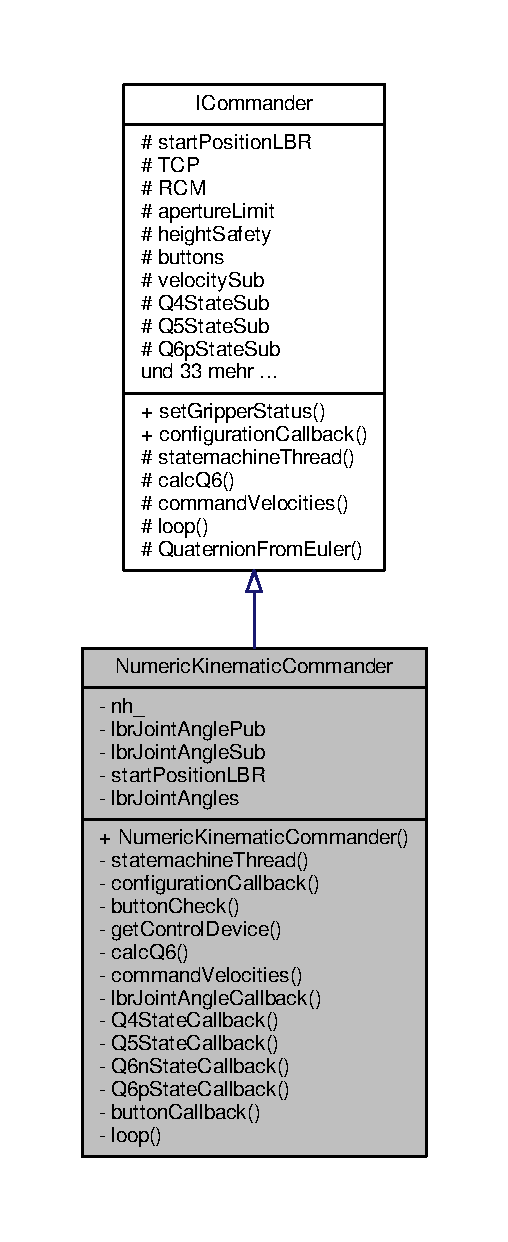
\includegraphics[height=550pt]{classNumericKinematicCommander__inherit__graph}
\end{center}
\end{figure}


Zusammengehörigkeiten von Numeric\-Kinematic\-Commander\-:
\nopagebreak
\begin{figure}[H]
\begin{center}
\leavevmode
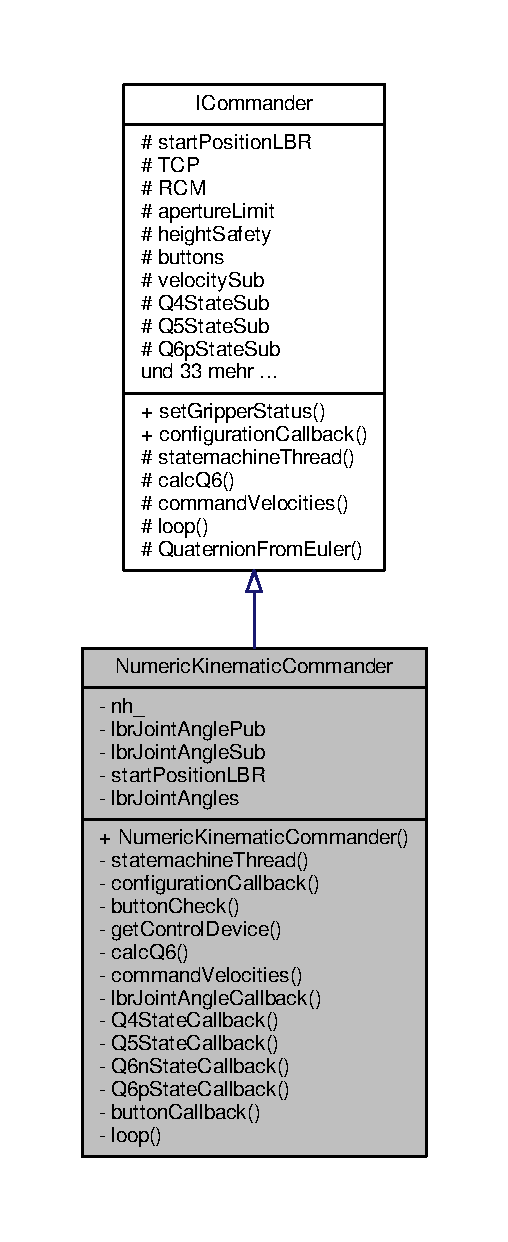
\includegraphics[height=550pt]{classNumericKinematicCommander__coll__graph}
\end{center}
\end{figure}
\subsection*{Öffentliche Methoden}
\begin{DoxyCompactItemize}
\item 
\hypertarget{classNumericKinematicCommander_ac9e6757a3e57c18e26076aa43e73da97}{{\bfseries Numeric\-Kinematic\-Commander} (ros\-::\-Node\-Handle \&nh, ros\-::\-Node\-Handle \&dr\-N\-H)}\label{classNumericKinematicCommander_ac9e6757a3e57c18e26076aa43e73da97}

\end{DoxyCompactItemize}
\subsection*{Private Methoden}
\begin{DoxyCompactItemize}
\item 
void \hyperlink{classNumericKinematicCommander_ad156c4e1d46ef88533b9c95ce553b9a0}{statemachine\-Thread} (const ros\-::\-Timer\-Event \&)
\begin{DoxyCompactList}\small\item\em Thread der alle 20ms aufgerufen wird und den Status an R\-O\-S\-Open\-I\-G\-T\-L\-Bridge schickt. \end{DoxyCompactList}\item 
void \hyperlink{classNumericKinematicCommander_a0c35190f764d4e1eb7aa8a2f3f8304a9}{configuration\-Callback} (masterslave\-::\-Master\-Slave\-Config \&config, uint32\-\_\-t level)
\begin{DoxyCompactList}\small\item\em Dynamic Reconfigure Callbackmethode. \end{DoxyCompactList}\item 
void \hyperlink{classNumericKinematicCommander_a3c13e655370bc0a9d4d19f2d37dff112}{button\-Check} ()
\begin{DoxyCompactList}\small\item\em Die Methode holt die Knopfkonfiguration vom Parameterserver. \end{DoxyCompactList}\item 
void \hyperlink{classNumericKinematicCommander_a05f5cb46b14a1379080ebfff17581cff}{get\-Control\-Device} ()
\begin{DoxyCompactList}\small\item\em Die Methode findet den Typ des Eingabegerätes auf dem Parameterserver. \end{DoxyCompactList}\item 
void \hyperlink{classNumericKinematicCommander_a86e5dee090c011b84df0adc60114b2cc}{calc\-Q6} ()
\begin{DoxyCompactList}\small\item\em Berechnet aus dem Gelenkwinkel Q6 die Gelenkwinkel Q6n und Q6p des Zangengreifers. \end{DoxyCompactList}\item 
void \hyperlink{classNumericKinematicCommander_aaf3d53306acb883148ceacfd9f65e32d}{command\-Velocities} ()
\begin{DoxyCompactList}\small\item\em Schickt die Gelenkwinkelgeschwindigkeiten an die Nodes der Antriebe des Werkzeuges. \end{DoxyCompactList}\item 
void \hyperlink{classNumericKinematicCommander_affceeb31adedb29f756e7b8804e5c5e7}{lbr\-Joint\-Angle\-Callback} (const sensor\-\_\-msgs\-::\-Joint\-State\-Const\-Ptr \&\hyperlink{classICommander_a72cb524deeb95b224db0242efc4728d4}{state}, int number)
\begin{DoxyCompactList}\small\item\em Multicallback für die Gelenkwinkel. \end{DoxyCompactList}\item 
\hypertarget{classNumericKinematicCommander_aff19777ef66a5931f9c138477063631d}{void {\bfseries Q4\-State\-Callback} (const sensor\-\_\-msgs\-::\-Joint\-State\-Const\-Ptr \&\hyperlink{classICommander_a72cb524deeb95b224db0242efc4728d4}{state})}\label{classNumericKinematicCommander_aff19777ef66a5931f9c138477063631d}

\item 
\hypertarget{classNumericKinematicCommander_a224d7ed8bbeeddd5291b8b64b1793ad8}{void {\bfseries Q5\-State\-Callback} (const sensor\-\_\-msgs\-::\-Joint\-State\-Const\-Ptr \&\hyperlink{classICommander_a72cb524deeb95b224db0242efc4728d4}{state})}\label{classNumericKinematicCommander_a224d7ed8bbeeddd5291b8b64b1793ad8}

\item 
\hypertarget{classNumericKinematicCommander_a8e36a50f45426dad83f8c9b4f551e623}{void {\bfseries Q6n\-State\-Callback} (const sensor\-\_\-msgs\-::\-Joint\-State\-Const\-Ptr \&\hyperlink{classICommander_a72cb524deeb95b224db0242efc4728d4}{state})}\label{classNumericKinematicCommander_a8e36a50f45426dad83f8c9b4f551e623}

\item 
\hypertarget{classNumericKinematicCommander_abf4374b164af476e526351ea413ebbc0}{void {\bfseries Q6p\-State\-Callback} (const sensor\-\_\-msgs\-::\-Joint\-State\-Const\-Ptr \&\hyperlink{classICommander_a72cb524deeb95b224db0242efc4728d4}{state})}\label{classNumericKinematicCommander_abf4374b164af476e526351ea413ebbc0}

\item 
\hypertarget{classNumericKinematicCommander_a27d9af68ec4d6d0f2dfbc00164856ed4}{void {\bfseries button\-Callback} (const masterslave\-::\-Button\-Const\-Ptr \&)}\label{classNumericKinematicCommander_a27d9af68ec4d6d0f2dfbc00164856ed4}

\item 
void \hyperlink{classNumericKinematicCommander_a95aed1cb2b8c58e82b4933972c4b2bf8}{loop} ()
\end{DoxyCompactItemize}
\subsection*{Private Attribute}
\begin{DoxyCompactItemize}
\item 
\hypertarget{classNumericKinematicCommander_a942510355ffa740a33a32601f6b7e6e2}{ros\-::\-Node\-Handle {\bfseries nh\-\_\-}}\label{classNumericKinematicCommander_a942510355ffa740a33a32601f6b7e6e2}

\item 
\hypertarget{classNumericKinematicCommander_aa930d89ec967e9099682755f31ea2488}{std\-::array$<$ ros\-::\-Publisher, 7 $>$ \hyperlink{classNumericKinematicCommander_aa930d89ec967e9099682755f31ea2488}{lbr\-Joint\-Angle\-Pub}}\label{classNumericKinematicCommander_aa930d89ec967e9099682755f31ea2488}

\begin{DoxyCompactList}\small\item\em Array mit den Sendern für die L\-B\-R-\/\-Gelenkwinkel. \end{DoxyCompactList}\item 
\hypertarget{classNumericKinematicCommander_adcfc69d33dbe0e7214ad5da711ff4010}{std\-::array$<$ ros\-::\-Subscriber, 7 $>$ \hyperlink{classNumericKinematicCommander_adcfc69d33dbe0e7214ad5da711ff4010}{lbr\-Joint\-Angle\-Sub}}\label{classNumericKinematicCommander_adcfc69d33dbe0e7214ad5da711ff4010}

\begin{DoxyCompactList}\small\item\em Array mit den Empfängern für die L\-B\-R-\/\-Gelenkwinkeln. \end{DoxyCompactList}\item 
\hypertarget{classNumericKinematicCommander_ad24e6088164ea771b0047cd1a2e0f53e}{Eigen\-::\-Affine3d \hyperlink{classNumericKinematicCommander_ad24e6088164ea771b0047cd1a2e0f53e}{start\-Position\-L\-B\-R}}\label{classNumericKinematicCommander_ad24e6088164ea771b0047cd1a2e0f53e}

\begin{DoxyCompactList}\small\item\em start\-Position\-L\-B\-R des L\-B\-Rs \end{DoxyCompactList}\item 
Eigen\-::\-Vector\-Xd \hyperlink{classNumericKinematicCommander_af12b3f3e1d3058dd7cf93b923ab6f13b}{lbr\-Joint\-Angles}
\end{DoxyCompactItemize}
\subsection*{Weitere Geerbte Elemente}


\subsection{Ausführliche Beschreibung}
Klasse, die sich um die R\-O\-S-\/\-Kommunikation für die numerisch bestimmte Kinematik kümmert. 

\begin{DoxyAuthor}{Autor}
Fabian Baier 
\end{DoxyAuthor}
\begin{DoxyDate}{Datum}
20.\-03.\-2016
\end{DoxyDate}
\begin{DoxySeeAlso}{Siehe auch}
\hyperlink{classICommander}{I\-Commander} 
\end{DoxySeeAlso}


\subsection{Dokumentation der Elementfunktionen}
\hypertarget{classNumericKinematicCommander_a3c13e655370bc0a9d4d19f2d37dff112}{\index{Numeric\-Kinematic\-Commander@{Numeric\-Kinematic\-Commander}!button\-Check@{button\-Check}}
\index{button\-Check@{button\-Check}!NumericKinematicCommander@{Numeric\-Kinematic\-Commander}}
\subsubsection[{button\-Check}]{\setlength{\rightskip}{0pt plus 5cm}Numeric\-Kinematic\-Commander\-::button\-Check (
\begin{DoxyParamCaption}
{}
\end{DoxyParamCaption}
)\hspace{0.3cm}{\ttfamily [private]}}}\label{classNumericKinematicCommander_a3c13e655370bc0a9d4d19f2d37dff112}


Die Methode holt die Knopfkonfiguration vom Parameterserver. 

\begin{DoxySeeAlso}{Siehe auch}
\hyperlink{classControlDevice}{Control\-Device} 
\end{DoxySeeAlso}
\hypertarget{classNumericKinematicCommander_a86e5dee090c011b84df0adc60114b2cc}{\index{Numeric\-Kinematic\-Commander@{Numeric\-Kinematic\-Commander}!calc\-Q6@{calc\-Q6}}
\index{calc\-Q6@{calc\-Q6}!NumericKinematicCommander@{Numeric\-Kinematic\-Commander}}
\subsubsection[{calc\-Q6}]{\setlength{\rightskip}{0pt plus 5cm}Numeric\-Kinematic\-Commander\-::calc\-Q6 (
\begin{DoxyParamCaption}
{}
\end{DoxyParamCaption}
)\hspace{0.3cm}{\ttfamily [private]}, {\ttfamily [virtual]}}}\label{classNumericKinematicCommander_a86e5dee090c011b84df0adc60114b2cc}


Berechnet aus dem Gelenkwinkel Q6 die Gelenkwinkel Q6n und Q6p des Zangengreifers. 

\begin{DoxySeeAlso}{Siehe auch}
\hyperlink{classICommander}{I\-Commander} 
\end{DoxySeeAlso}


Implementiert \hyperlink{classICommander_a1967688a309974862c4a81b5fe04c3eb}{I\-Commander}.

\hypertarget{classNumericKinematicCommander_aaf3d53306acb883148ceacfd9f65e32d}{\index{Numeric\-Kinematic\-Commander@{Numeric\-Kinematic\-Commander}!command\-Velocities@{command\-Velocities}}
\index{command\-Velocities@{command\-Velocities}!NumericKinematicCommander@{Numeric\-Kinematic\-Commander}}
\subsubsection[{command\-Velocities}]{\setlength{\rightskip}{0pt plus 5cm}Numeric\-Kinematic\-Commander\-::command\-Velocities (
\begin{DoxyParamCaption}
{}
\end{DoxyParamCaption}
)\hspace{0.3cm}{\ttfamily [private]}, {\ttfamily [virtual]}}}\label{classNumericKinematicCommander_aaf3d53306acb883148ceacfd9f65e32d}


Schickt die Gelenkwinkelgeschwindigkeiten an die Nodes der Antriebe des Werkzeuges. 

\begin{DoxySeeAlso}{Siehe auch}
\hyperlink{classICommander}{I\-Commander} 
\end{DoxySeeAlso}


Implementiert \hyperlink{classICommander_a43c10dd80f4815afd4058226450c7af3}{I\-Commander}.

\hypertarget{classNumericKinematicCommander_a0c35190f764d4e1eb7aa8a2f3f8304a9}{\index{Numeric\-Kinematic\-Commander@{Numeric\-Kinematic\-Commander}!configuration\-Callback@{configuration\-Callback}}
\index{configuration\-Callback@{configuration\-Callback}!NumericKinematicCommander@{Numeric\-Kinematic\-Commander}}
\subsubsection[{configuration\-Callback}]{\setlength{\rightskip}{0pt plus 5cm}Numeric\-Kinematic\-Commander\-::configuration\-Callback (
\begin{DoxyParamCaption}
\item[{masterslave\-::\-Master\-Slave\-Config \&}]{config, }
\item[{uint32\-\_\-t}]{level}
\end{DoxyParamCaption}
)\hspace{0.3cm}{\ttfamily [private]}}}\label{classNumericKinematicCommander_a0c35190f764d4e1eb7aa8a2f3f8304a9}


Dynamic Reconfigure Callbackmethode. 


\begin{DoxyParams}{Parameter}
{\em config} & Dynamic Reconfigure Struktur \\
\hline
{\em level} & Bitmaske \\
\hline
\end{DoxyParams}
\begin{DoxySeeAlso}{Siehe auch}
\hyperlink{classGeometricKinematicCommander}{Geometric\-Kinematic\-Commander}, Master\-Slave\-Config.\-cfg 
\end{DoxySeeAlso}
\hypertarget{classNumericKinematicCommander_a05f5cb46b14a1379080ebfff17581cff}{\index{Numeric\-Kinematic\-Commander@{Numeric\-Kinematic\-Commander}!get\-Control\-Device@{get\-Control\-Device}}
\index{get\-Control\-Device@{get\-Control\-Device}!NumericKinematicCommander@{Numeric\-Kinematic\-Commander}}
\subsubsection[{get\-Control\-Device}]{\setlength{\rightskip}{0pt plus 5cm}Numeric\-Kinematic\-Commander\-::get\-Control\-Device (
\begin{DoxyParamCaption}
{}
\end{DoxyParamCaption}
)\hspace{0.3cm}{\ttfamily [private]}}}\label{classNumericKinematicCommander_a05f5cb46b14a1379080ebfff17581cff}


Die Methode findet den Typ des Eingabegerätes auf dem Parameterserver. 

\begin{DoxySeeAlso}{Siehe auch}
\hyperlink{classControlDevice}{Control\-Device} 
\end{DoxySeeAlso}
\hypertarget{classNumericKinematicCommander_affceeb31adedb29f756e7b8804e5c5e7}{\index{Numeric\-Kinematic\-Commander@{Numeric\-Kinematic\-Commander}!lbr\-Joint\-Angle\-Callback@{lbr\-Joint\-Angle\-Callback}}
\index{lbr\-Joint\-Angle\-Callback@{lbr\-Joint\-Angle\-Callback}!NumericKinematicCommander@{Numeric\-Kinematic\-Commander}}
\subsubsection[{lbr\-Joint\-Angle\-Callback}]{\setlength{\rightskip}{0pt plus 5cm}Numeric\-Kinematic\-Commander\-::lbr\-Joint\-Angle\-Callback (
\begin{DoxyParamCaption}
\item[{const sensor\-\_\-msgs\-::\-Joint\-State\-Const\-Ptr \&}]{state, }
\item[{int}]{number}
\end{DoxyParamCaption}
)\hspace{0.3cm}{\ttfamily [private]}}}\label{classNumericKinematicCommander_affceeb31adedb29f756e7b8804e5c5e7}


Multicallback für die Gelenkwinkel. 


\begin{DoxyParams}{Parameter}
{\em state} & \\
\hline
{\em number} & \\
\hline
\end{DoxyParams}
\hypertarget{classNumericKinematicCommander_a95aed1cb2b8c58e82b4933972c4b2bf8}{\index{Numeric\-Kinematic\-Commander@{Numeric\-Kinematic\-Commander}!loop@{loop}}
\index{loop@{loop}!NumericKinematicCommander@{Numeric\-Kinematic\-Commander}}
\subsubsection[{loop}]{\setlength{\rightskip}{0pt plus 5cm}Numeric\-Kinematic\-Commander\-::loop (
\begin{DoxyParamCaption}
{}
\end{DoxyParamCaption}
)\hspace{0.3cm}{\ttfamily [private]}, {\ttfamily [virtual]}}}\label{classNumericKinematicCommander_a95aed1cb2b8c58e82b4933972c4b2bf8}
\begin{DoxySeeAlso}{Siehe auch}
\hyperlink{classICommander}{I\-Commander} 
\end{DoxySeeAlso}


Implementiert \hyperlink{classICommander_aa5f882f46d3629fa754162a9ee11984c}{I\-Commander}.

\hypertarget{classNumericKinematicCommander_ad156c4e1d46ef88533b9c95ce553b9a0}{\index{Numeric\-Kinematic\-Commander@{Numeric\-Kinematic\-Commander}!statemachine\-Thread@{statemachine\-Thread}}
\index{statemachine\-Thread@{statemachine\-Thread}!NumericKinematicCommander@{Numeric\-Kinematic\-Commander}}
\subsubsection[{statemachine\-Thread}]{\setlength{\rightskip}{0pt plus 5cm}Numeric\-Kinematic\-Commander\-::statemachine\-Thread (
\begin{DoxyParamCaption}
\item[{const ros\-::\-Timer\-Event \&}]{}
\end{DoxyParamCaption}
)\hspace{0.3cm}{\ttfamily [private]}, {\ttfamily [virtual]}}}\label{classNumericKinematicCommander_ad156c4e1d46ef88533b9c95ce553b9a0}


Thread der alle 20ms aufgerufen wird und den Status an R\-O\-S\-Open\-I\-G\-T\-L\-Bridge schickt. 

\begin{DoxySeeAlso}{Siehe auch}
\hyperlink{classICommander}{I\-Commander} 
\end{DoxySeeAlso}


Implementiert \hyperlink{classICommander_abcacd07f49f646d08e1722a1df08b8ce}{I\-Commander}.



\subsection{Dokumentation der Datenelemente}
\hypertarget{classNumericKinematicCommander_af12b3f3e1d3058dd7cf93b923ab6f13b}{\index{Numeric\-Kinematic\-Commander@{Numeric\-Kinematic\-Commander}!lbr\-Joint\-Angles@{lbr\-Joint\-Angles}}
\index{lbr\-Joint\-Angles@{lbr\-Joint\-Angles}!NumericKinematicCommander@{Numeric\-Kinematic\-Commander}}
\subsubsection[{lbr\-Joint\-Angles}]{\setlength{\rightskip}{0pt plus 5cm}Numeric\-Kinematic\-Commander\-::lbr\-Joint\-Angles\hspace{0.3cm}{\ttfamily [private]}}}\label{classNumericKinematicCommander_af12b3f3e1d3058dd7cf93b923ab6f13b}
\begin{DoxyRefDesc}{Noch zu erledigen}
\item[\hyperlink{todo__todo000007}{Noch zu erledigen}]check ob noch benötigt \end{DoxyRefDesc}


Die Dokumentation für diese Klasse wurde erzeugt aufgrund der Datei\-:\begin{DoxyCompactItemize}
\item 
include/masterslave/commander/\hyperlink{NumericKinematicCommander_8h}{Numeric\-Kinematic\-Commander.\-h}\end{DoxyCompactItemize}

\hypertarget{classPTPTrajectory}{\section{P\-T\-P\-Trajectory Klassenreferenz}
\label{classPTPTrajectory}\index{P\-T\-P\-Trajectory@{P\-T\-P\-Trajectory}}
}


Klassendiagramm für P\-T\-P\-Trajectory\-:
\nopagebreak
\begin{figure}[H]
\begin{center}
\leavevmode
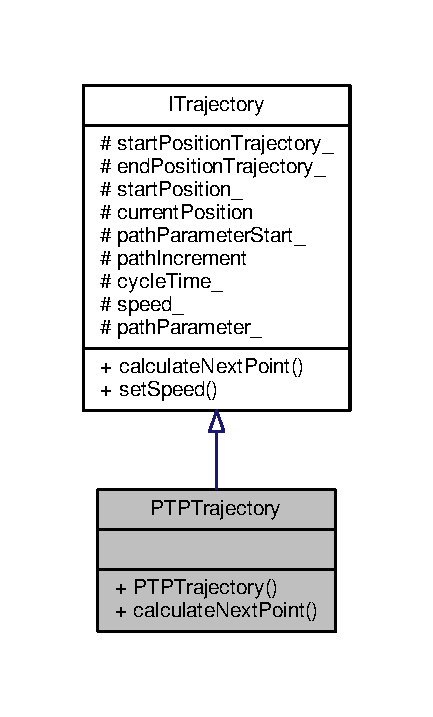
\includegraphics[width=208pt]{classPTPTrajectory__inherit__graph}
\end{center}
\end{figure}


Zusammengehörigkeiten von P\-T\-P\-Trajectory\-:
\nopagebreak
\begin{figure}[H]
\begin{center}
\leavevmode
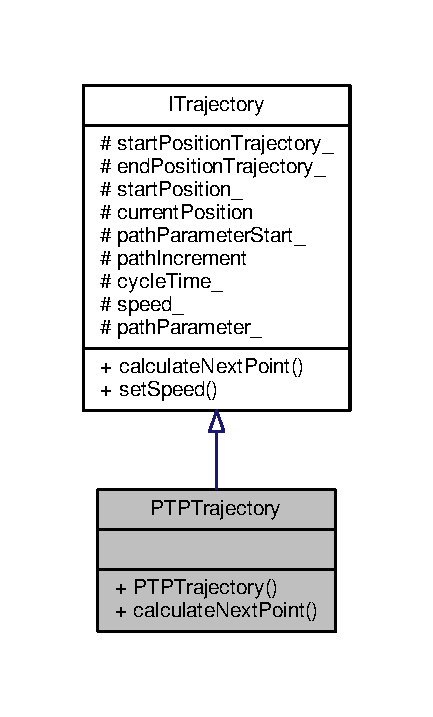
\includegraphics[width=208pt]{classPTPTrajectory__coll__graph}
\end{center}
\end{figure}
\subsection*{Öffentliche Methoden}
\begin{DoxyCompactItemize}
\item 
\hypertarget{classPTPTrajectory_ad2815fd1e9bdf070759947237ac8961c}{{\bfseries P\-T\-P\-Trajectory} (Eigen\-::\-Affine3d start\-Point, Eigen\-::\-Vector3d R\-C\-M, Eigen\-::\-Vector3d first\-Point, Eigen\-::\-Vector3d second\-Point, int speed, double cycle\-Time)}\label{classPTPTrajectory_ad2815fd1e9bdf070759947237ac8961c}

\item 
Eigen\-::\-Affine3d \hyperlink{classPTPTrajectory_a6663a421aba9674577cdc014c8cb8b77}{calculate\-Next\-Point} ()
\end{DoxyCompactItemize}
\subsection*{Weitere Geerbte Elemente}


\subsection{Dokumentation der Elementfunktionen}
\hypertarget{classPTPTrajectory_a6663a421aba9674577cdc014c8cb8b77}{\index{P\-T\-P\-Trajectory@{P\-T\-P\-Trajectory}!calculate\-Next\-Point@{calculate\-Next\-Point}}
\index{calculate\-Next\-Point@{calculate\-Next\-Point}!PTPTrajectory@{P\-T\-P\-Trajectory}}
\subsubsection[{calculate\-Next\-Point}]{\setlength{\rightskip}{0pt plus 5cm}P\-T\-P\-Trajectory\-::calculate\-Next\-Point (
\begin{DoxyParamCaption}
{}
\end{DoxyParamCaption}
)\hspace{0.3cm}{\ttfamily [virtual]}}}\label{classPTPTrajectory_a6663a421aba9674577cdc014c8cb8b77}
\begin{DoxySeeAlso}{Siehe auch}
\hyperlink{classITrajectory}{I\-Trajectory} 
\end{DoxySeeAlso}


Implementiert \hyperlink{classITrajectory_a7baff9fb2fc20987e9469d736a90406b}{I\-Trajectory}.



Die Dokumentation für diese Klasse wurde erzeugt aufgrund der Datei\-:\begin{DoxyCompactItemize}
\item 
include/masterslave/manipulation/trajectory/P\-T\-P\-Trajectory.\-h\end{DoxyCompactItemize}

\hypertarget{classRosOpenIgtlBridge}{\section{Ros\-Open\-Igtl\-Bridge Klassenreferenz}
\label{classRosOpenIgtlBridge}\index{Ros\-Open\-Igtl\-Bridge@{Ros\-Open\-Igtl\-Bridge}}
}


Eine R\-O\-S-\/\-Node zur Kommunikation zwischen R\-O\-S und dem L\-B\-R iiwa, welche über das Open\-I\-G\-T\-Link-\/\-Protokoll durchgeführt.  




{\ttfamily \#include $<$Ros\-Open\-I\-G\-T\-L\-Bridge.\-h$>$}



Zusammengehörigkeiten von Ros\-Open\-Igtl\-Bridge\-:
\nopagebreak
\begin{figure}[H]
\begin{center}
\leavevmode
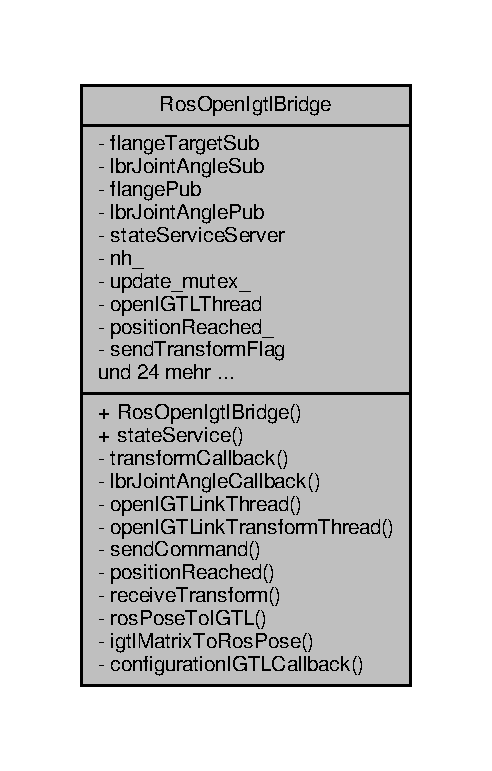
\includegraphics[width=236pt]{classRosOpenIgtlBridge__coll__graph}
\end{center}
\end{figure}
\subsection*{Öffentliche Methoden}
\begin{DoxyCompactItemize}
\item 
\hypertarget{classRosOpenIgtlBridge_a46b348ca4dee935c87eea78653046cc0}{{\bfseries Ros\-Open\-Igtl\-Bridge} (ros\-::\-Node\-Handle)}\label{classRosOpenIgtlBridge_a46b348ca4dee935c87eea78653046cc0}

\item 
bool \hyperlink{classRosOpenIgtlBridge_ac8d2f37fe82fb7d0496d937920f48db6}{state\-Service} (masterslave\-::\-Open\-I\-G\-T\-L\-State\-Service\-::\-Request \&req, masterslave\-::\-Open\-I\-G\-T\-L\-State\-Service\-::\-Response \&res)
\begin{DoxyCompactList}\small\item\em Dieses ist eine Callback-\/\-Methode, die aufgerufen wird, wenn der Zustand des Roboters geändert werden soll Mögliche Zustände\-: I\-D\-L\-E, F\-R\-E\-E, M\-O\-V\-E\-\_\-\-T\-O\-\_\-\-P\-O\-S\-E. \end{DoxyCompactList}\end{DoxyCompactItemize}
\subsection*{Private Methoden}
\begin{DoxyCompactItemize}
\item 
void \hyperlink{classRosOpenIgtlBridge_a654f0a40a6e10644de54f0a47efcbb9d}{transform\-Callback} (geometry\-\_\-msgs\-::\-Pose\-Stamped\-Const\-Ptr transform)
\begin{DoxyCompactList}\small\item\em In der Methode werden die Sollpositionen aus der geometrischen Kinematik entgegen genommen. \end{DoxyCompactList}\item 
void \hyperlink{classRosOpenIgtlBridge_a8f02e3d18f60754c8d282db55eaed4c2}{lbr\-Joint\-Angle\-Callback} (const std\-\_\-msgs\-::\-Float64\-Const\-Ptr \&joint\-Angle, int number)
\begin{DoxyCompactList}\small\item\em In dieser Methode werden die. \end{DoxyCompactList}\item 
\hypertarget{classRosOpenIgtlBridge_adb7ae9d852083bcb79e2172ecc380cd6}{void \hyperlink{classRosOpenIgtlBridge_adb7ae9d852083bcb79e2172ecc380cd6}{open\-I\-G\-T\-Link\-Thread} ()}\label{classRosOpenIgtlBridge_adb7ae9d852083bcb79e2172ecc380cd6}

\begin{DoxyCompactList}\small\item\em zyklische Versendung der durch R\-O\-S empfangenen Daten über einen Open\-I\-G\-T\-Link-\/\-Clientsocket \end{DoxyCompactList}\item 
\hypertarget{classRosOpenIgtlBridge_a7477fb39f8246408e1e82e69fb17e866}{void \hyperlink{classRosOpenIgtlBridge_a7477fb39f8246408e1e82e69fb17e866}{open\-I\-G\-T\-Link\-Transform\-Thread} ()}\label{classRosOpenIgtlBridge_a7477fb39f8246408e1e82e69fb17e866}

\begin{DoxyCompactList}\small\item\em zyklischer Empfang der Gelenktransformationen bzw. der Endeffektorlage des L\-B\-R \end{DoxyCompactList}\item 
int \hyperlink{classRosOpenIgtlBridge_a741e133a8fbd1fed1508ec636723de5a}{send\-Command} (igtl\-::\-Client\-Socket\-::\-Pointer \&socket, std\-::string command)
\begin{DoxyCompactList}\small\item\em Methode zum Versenden von std\-::strings über den Open\-I\-G\-T\-Link-\/\-Socket. \end{DoxyCompactList}\item 
int \hyperlink{classRosOpenIgtlBridge_aa375549cb5b12c850c363a992eb87340}{position\-Reached} (igtl\-::\-Client\-Socket\-::\-Pointer \&socket, igtl\-::\-Message\-Base\-::\-Pointer \&msg\-Header)
\begin{DoxyCompactList}\small\item\em Überwachung, ob die angegebene Zielpose bereits erreicht wurde. \end{DoxyCompactList}\item 
int \hyperlink{classRosOpenIgtlBridge_a051b146bbe2dd3d1ea63677efeb62155}{receive\-Transform} (igtl\-::\-Client\-Socket\-::\-Pointer \&socket, igtl\-::\-Message\-Base\-::\-Pointer \&msg\-Header)
\begin{DoxyCompactList}\small\item\em Empfang der Transformationsnachrichten. \end{DoxyCompactList}\item 
std\-::string \hyperlink{classRosOpenIgtlBridge_a99c187746613fa369b79e73c2ccb7c62}{ros\-Pose\-To\-I\-G\-T\-L} (geometry\-\_\-msgs\-::\-Pose pose)
\begin{DoxyCompactList}\small\item\em Hilfsfunktion um eine geometry\-\_\-msgs\-::\-Pose in einen String zu verwandeln, um diesen anschließend über Open\-I\-G\-T\-Link zu versenden. \end{DoxyCompactList}\item 
geometry\-\_\-msgs\-::\-Pose \hyperlink{classRosOpenIgtlBridge_ac9e20d912d93a8c7723511a255033cae}{igtl\-Matrix\-To\-Ros\-Pose} (igtl\-::\-Matrix4x4 \&igtl\-Matrix)
\begin{DoxyCompactList}\small\item\em Hilfsfunktion um eine igtl\-::\-Matrix4x4 in eine geometry\-\_\-msgs\-::\-Pose zu wandeln und diese in R\-O\-S zu übertragen. \end{DoxyCompactList}\item 
void \hyperlink{classRosOpenIgtlBridge_a6efbb5bd82d24454e040ea03549d4426}{configuration\-I\-G\-T\-L\-Callback} (masterslave\-::\-Ros\-Open\-I\-G\-T\-L\-Bridge\-Config \&config, uint32\-\_\-t level)
\begin{DoxyCompactList}\small\item\em Callbackmethode für dynamic reconfigure. \end{DoxyCompactList}\end{DoxyCompactItemize}
\subsection*{Private Attribute}
\begin{DoxyCompactItemize}
\item 
\hypertarget{classRosOpenIgtlBridge_a7f2d1b92afa2a0e5c5a96abf15e559fc}{ros\-::\-Subscriber \hyperlink{classRosOpenIgtlBridge_a7f2d1b92afa2a0e5c5a96abf15e559fc}{flange\-Target\-Sub}}\label{classRosOpenIgtlBridge_a7f2d1b92afa2a0e5c5a96abf15e559fc}

\begin{DoxyCompactList}\small\item\em Empfänger für Solllagen des Endeffektors in R\-O\-S. \end{DoxyCompactList}\item 
\hypertarget{classRosOpenIgtlBridge_a2cec061ef757bb52933768c2dd3fde1e}{std\-::array$<$ ros\-::\-Subscriber, 7 $>$ \hyperlink{classRosOpenIgtlBridge_a2cec061ef757bb52933768c2dd3fde1e}{lbr\-Joint\-Angle\-Sub}}\label{classRosOpenIgtlBridge_a2cec061ef757bb52933768c2dd3fde1e}

\begin{DoxyCompactList}\small\item\em Empfänger für die gewünschte Gelenkwinkelposition des L\-B\-R iiwa in R\-O\-S. \end{DoxyCompactList}\item 
\hypertarget{classRosOpenIgtlBridge_ac97a67c4e0f7afbc2811acb3857464e3}{ros\-::\-Publisher \hyperlink{classRosOpenIgtlBridge_ac97a67c4e0f7afbc2811acb3857464e3}{flange\-Pub}}\label{classRosOpenIgtlBridge_ac97a67c4e0f7afbc2811acb3857464e3}

\begin{DoxyCompactList}\small\item\em Sender für die eingenommene Endeffektorlage in R\-O\-S. \end{DoxyCompactList}\item 
\hypertarget{classRosOpenIgtlBridge_a777b34678fb3d17d5ad177b1e7ec1225}{std\-::array$<$ ros\-::\-Publisher, 7 $>$ \hyperlink{classRosOpenIgtlBridge_a777b34678fb3d17d5ad177b1e7ec1225}{lbr\-Joint\-Angle\-Pub}}\label{classRosOpenIgtlBridge_a777b34678fb3d17d5ad177b1e7ec1225}

\begin{DoxyCompactList}\small\item\em Sender für die aktuelle Gelenkwinkelkonfiguration des L\-B\-R iiwa. \end{DoxyCompactList}\item 
ros\-::\-Service\-Server \hyperlink{classRosOpenIgtlBridge_ad7c6b0430970a8faf6cc9e934d6f889e}{state\-Service\-Server}
\begin{DoxyCompactList}\small\item\em Objekt zur Bereitstellung des state\-Services. \end{DoxyCompactList}\item 
\hypertarget{classRosOpenIgtlBridge_a69a4a87ec19cd98435f0376f58f3e525}{ros\-::\-Node\-Handle {\bfseries nh\-\_\-}}\label{classRosOpenIgtlBridge_a69a4a87ec19cd98435f0376f58f3e525}

\item 
\hypertarget{classRosOpenIgtlBridge_ac28588689dc275b6b06efa56e9bfbcc3}{boost\-::mutex {\bfseries update\-\_\-mutex\-\_\-}}\label{classRosOpenIgtlBridge_ac28588689dc275b6b06efa56e9bfbcc3}

\item 
\hypertarget{classRosOpenIgtlBridge_ab7c09ef893ace60f12429b6df7d295e6}{boost\-::thread {\bfseries open\-I\-G\-T\-L\-Thread}}\label{classRosOpenIgtlBridge_ab7c09ef893ace60f12429b6df7d295e6}

\item 
\hypertarget{classRosOpenIgtlBridge_a1a2f941f4f0fcb4fee19f01acc3ff32b}{int \hyperlink{classRosOpenIgtlBridge_a1a2f941f4f0fcb4fee19f01acc3ff32b}{position\-Reached\-\_\-}}\label{classRosOpenIgtlBridge_a1a2f941f4f0fcb4fee19f01acc3ff32b}

\begin{DoxyCompactList}\small\item\em wurde die Pose durch den L\-B\-R erfolgreich angefahren? \end{DoxyCompactList}\item 
\hypertarget{classRosOpenIgtlBridge_a1b105e3199f1f2faf21b2479c4518db1}{bool \hyperlink{classRosOpenIgtlBridge_a1b105e3199f1f2faf21b2479c4518db1}{send\-Transform\-Flag} \{false\}}\label{classRosOpenIgtlBridge_a1b105e3199f1f2faf21b2479c4518db1}

\begin{DoxyCompactList}\small\item\em wurde die aktuell vorliegende Solllage des L\-B\-R iiwa schon über Open\-I\-G\-T\-Link übertragen? \end{DoxyCompactList}\item 
\hypertarget{classRosOpenIgtlBridge_a0517326bc17e781461b2a1391298f620}{boost\-::mutex {\bfseries transform\-Update\-Mutex\-\_\-}}\label{classRosOpenIgtlBridge_a0517326bc17e781461b2a1391298f620}

\item 
\hypertarget{classRosOpenIgtlBridge_a8dbc016aacf3ff2caad058ec50a96e77}{igtl\-::\-Matrix4x4 \hyperlink{classRosOpenIgtlBridge_a8dbc016aacf3ff2caad058ec50a96e77}{T\-\_\-\-F\-L}}\label{classRosOpenIgtlBridge_a8dbc016aacf3ff2caad058ec50a96e77}

\begin{DoxyCompactList}\small\item\em Solllage des Endeffektors des L\-B\-R. \end{DoxyCompactList}\item 
\hypertarget{classRosOpenIgtlBridge_ace49281b853f92fbd9decbaa2dcd5b70}{igtl\-::\-Matrix4x4 \hyperlink{classRosOpenIgtlBridge_ace49281b853f92fbd9decbaa2dcd5b70}{T\-\_\-\-F\-L\-\_\-new}}\label{classRosOpenIgtlBridge_ace49281b853f92fbd9decbaa2dcd5b70}

\begin{DoxyCompactList}\small\item\em aktuell empfangene Lage des Endeffektors des L\-B\-R \end{DoxyCompactList}\item 
geometry\-\_\-msgs\-::\-Pose \hyperlink{classRosOpenIgtlBridge_a43a57e8fe72fa4a233b744a3576310da}{pose\-F\-L}
\begin{DoxyCompactList}\small\item\em Solllage des Endeffektors im R\-O\-S-\/konformen Variablentyp. \end{DoxyCompactList}\item 
geometry\-\_\-msgs\-::\-Pose \hyperlink{classRosOpenIgtlBridge_afee0e87dfe158f8980081554b3f8dac2}{pose\-F\-L\-\_\-new}
\begin{DoxyCompactList}\small\item\em aktuell empfangene Lage des Endeffektors des L\-B\-R im R\-O\-S-\/konformen Variablentyp \end{DoxyCompactList}\item 
\hypertarget{classRosOpenIgtlBridge_a4cb6ad04d4d51de2228ba529efb85a89}{Eigen\-::\-Vector\-Xd \hyperlink{classRosOpenIgtlBridge_a4cb6ad04d4d51de2228ba529efb85a89}{joint\-Angles}}\label{classRosOpenIgtlBridge_a4cb6ad04d4d51de2228ba529efb85a89}

\begin{DoxyCompactList}\small\item\em gewünschte Gelenkwinkel des L\-B\-R iiwa \end{DoxyCompactList}\item 
\hypertarget{classRosOpenIgtlBridge_a2fa9f49baaba81330c1d19967754738d}{Eigen\-::\-Vector\-Xd \hyperlink{classRosOpenIgtlBridge_a2fa9f49baaba81330c1d19967754738d}{joint\-Angles\-\_\-new}}\label{classRosOpenIgtlBridge_a2fa9f49baaba81330c1d19967754738d}

\begin{DoxyCompactList}\small\item\em aktuell empfangene Gelenkwinkel des L\-B\-R iiwa \end{DoxyCompactList}\item 
igtl\-::\-Client\-Socket\-::\-Pointer \hyperlink{classRosOpenIgtlBridge_a06df713358aa522ed6dd363d78bb8def}{command\-Socket\-\_\-}
\begin{DoxyCompactList}\small\item\em Socket über den Gelenkwinkel oder Endeffektorsolllagen kommandiert werden mit I\-P und Port als Konstanten. \end{DoxyCompactList}\item 
\hypertarget{classRosOpenIgtlBridge_a18105c3a5c5cbb4b71bb1ae5c9ee103b}{const int {\bfseries C\-O\-M\-M\-A\-N\-D\-\_\-\-P\-O\-R\-T} \{49001\}}\label{classRosOpenIgtlBridge_a18105c3a5c5cbb4b71bb1ae5c9ee103b}

\item 
\hypertarget{classRosOpenIgtlBridge_a808bb79742c62aaea43bf539f1ac677a}{const char $\ast$ {\bfseries C\-O\-M\-M\-A\-N\-D\-\_\-\-I\-P} \{\char`\"{}172.\-31.\-1.\-147\char`\"{}\}}\label{classRosOpenIgtlBridge_a808bb79742c62aaea43bf539f1ac677a}

\item 
\hypertarget{classRosOpenIgtlBridge_ad0b28209a738b231f97717f234e380ec}{int \hyperlink{classRosOpenIgtlBridge_ad0b28209a738b231f97717f234e380ec}{r\-Command}}\label{classRosOpenIgtlBridge_ad0b28209a738b231f97717f234e380ec}

\begin{DoxyCompactList}\small\item\em Status des Sockets. \end{DoxyCompactList}\item 
\hypertarget{classRosOpenIgtlBridge_a8b21f91b5ef292bbc6a3be6c3d987602}{unsigned long long \hyperlink{classRosOpenIgtlBridge_a8b21f91b5ef292bbc6a3be6c3d987602}{C\-M\-D\-\_\-\-U\-I\-D} \{0\}}\label{classRosOpenIgtlBridge_a8b21f91b5ef292bbc6a3be6c3d987602}

\begin{DoxyCompactList}\small\item\em Nummer des übermittelten Datenpakets. \end{DoxyCompactList}\item 
igtl\-::\-Client\-Socket\-::\-Pointer \hyperlink{classRosOpenIgtlBridge_ac1cd3818cb07542c4534f7dfdb3b0258}{transform\-Socket\-\_\-}
\begin{DoxyCompactList}\small\item\em Socket über den die Gelenktransformationen und die Endeffektorlage empfangen werden mit I\-P und Port als Konstanten. \end{DoxyCompactList}\item 
\hypertarget{classRosOpenIgtlBridge_a3e034f310cd5ccc3a3c53986b13cbb16}{const int {\bfseries T\-R\-A\-N\-S\-F\-O\-R\-M\-\_\-\-P\-O\-R\-T} \{49002\}}\label{classRosOpenIgtlBridge_a3e034f310cd5ccc3a3c53986b13cbb16}

\item 
\hypertarget{classRosOpenIgtlBridge_a9f4462ec60da6213f9c8e3e5aa804d25}{const char $\ast$ {\bfseries T\-R\-A\-N\-S\-F\-O\-R\-M\-\_\-\-I\-P} \{\char`\"{}172.\-31.\-1.\-147\char`\"{}\}}\label{classRosOpenIgtlBridge_a9f4462ec60da6213f9c8e3e5aa804d25}

\item 
\hypertarget{classRosOpenIgtlBridge_a48389d9a54fe5bb8dde3bd6b44ca85c9}{int \hyperlink{classRosOpenIgtlBridge_a48389d9a54fe5bb8dde3bd6b44ca85c9}{r\-Transform}}\label{classRosOpenIgtlBridge_a48389d9a54fe5bb8dde3bd6b44ca85c9}

\begin{DoxyCompactList}\small\item\em Status des Empfangssockets. \end{DoxyCompactList}\item 
\hypertarget{classRosOpenIgtlBridge_a691ab680de3cd5e45c7ac40816b732a6}{std\-::string {\bfseries open\-I\-G\-T\-L\-Command\-String}}\label{classRosOpenIgtlBridge_a691ab680de3cd5e45c7ac40816b732a6}

\item 
\hypertarget{classRosOpenIgtlBridge_a0a5db0b04705372961630bb4c027695c}{std\-::string {\bfseries state\-String}}\label{classRosOpenIgtlBridge_a0a5db0b04705372961630bb4c027695c}

\item 
\hypertarget{classRosOpenIgtlBridge_a2ea062eeab4c7158b07ee976503ef043}{double {\bfseries sample\-Time\-\_\-}}\label{classRosOpenIgtlBridge_a2ea062eeab4c7158b07ee976503ef043}

\item 
\hypertarget{classRosOpenIgtlBridge_a38daf9dd118068189027ba9ba94c4490}{bool {\bfseries stop\-\_\-}}\label{classRosOpenIgtlBridge_a38daf9dd118068189027ba9ba94c4490}

\item 
\hypertarget{classRosOpenIgtlBridge_ac71d24bebd6fc3271705f429e72e3073}{bool {\bfseries start\-\_\-}}\label{classRosOpenIgtlBridge_ac71d24bebd6fc3271705f429e72e3073}

\item 
\hypertarget{classRosOpenIgtlBridge_a739a2b4feace96f89628c36a9357ccfe}{bool {\bfseries transform\-Received\-\_\-} \{false\}}\label{classRosOpenIgtlBridge_a739a2b4feace96f89628c36a9357ccfe}

\item 
\hypertarget{classRosOpenIgtlBridge_aab902594c15e9b69c6f0b7bdb2c2814c}{bool {\bfseries ros\-Transform\-Received\-\_\-} \{false\}}\label{classRosOpenIgtlBridge_aab902594c15e9b69c6f0b7bdb2c2814c}

\item 
\hypertarget{classRosOpenIgtlBridge_a701bc14cf735f3e01d807e8c7074d0e5}{const unsigned int {\bfseries C\-O\-N\-N\-E\-C\-T\-I\-O\-N\-\_\-\-T\-I\-M\-E\-O\-U\-T} \{30\}}\label{classRosOpenIgtlBridge_a701bc14cf735f3e01d807e8c7074d0e5}

\end{DoxyCompactItemize}


\subsection{Ausführliche Beschreibung}
Eine R\-O\-S-\/\-Node zur Kommunikation zwischen R\-O\-S und dem L\-B\-R iiwa, welche über das Open\-I\-G\-T\-Link-\/\-Protokoll durchgeführt. 

\begin{DoxyAuthor}{Autor}
Fabian Baier 
\end{DoxyAuthor}
\begin{DoxyDate}{Datum}
19.\-03.\-2016
\end{DoxyDate}
\begin{DoxyVersion}{Version}
0.\-3 
\end{DoxyVersion}


\subsection{Dokumentation der Elementfunktionen}
\hypertarget{classRosOpenIgtlBridge_a6efbb5bd82d24454e040ea03549d4426}{\index{Ros\-Open\-Igtl\-Bridge@{Ros\-Open\-Igtl\-Bridge}!configuration\-I\-G\-T\-L\-Callback@{configuration\-I\-G\-T\-L\-Callback}}
\index{configuration\-I\-G\-T\-L\-Callback@{configuration\-I\-G\-T\-L\-Callback}!RosOpenIgtlBridge@{Ros\-Open\-Igtl\-Bridge}}
\subsubsection[{configuration\-I\-G\-T\-L\-Callback}]{\setlength{\rightskip}{0pt plus 5cm}Ros\-Open\-Igtl\-Bridge\-::configuration\-I\-G\-T\-L\-Callback (
\begin{DoxyParamCaption}
\item[{masterslave\-::\-Ros\-Open\-I\-G\-T\-L\-Bridge\-Config \&}]{config, }
\item[{uint32\-\_\-t}]{level}
\end{DoxyParamCaption}
)\hspace{0.3cm}{\ttfamily [private]}}}\label{classRosOpenIgtlBridge_a6efbb5bd82d24454e040ea03549d4426}


Callbackmethode für dynamic reconfigure. 


\begin{DoxyParams}{Parameter}
{\em config} & Konfiguration von dynamic reconfigure \\
\hline
{\em level} & Bitmaske zur Maskierung einzelner Einstellungen \\
\hline
\end{DoxyParams}
\begin{DoxySeeAlso}{Siehe auch}
Ros\-Open\-I\-G\-T\-L\-Bridge.\-cfg 
\end{DoxySeeAlso}
\hypertarget{classRosOpenIgtlBridge_ac9e20d912d93a8c7723511a255033cae}{\index{Ros\-Open\-Igtl\-Bridge@{Ros\-Open\-Igtl\-Bridge}!igtl\-Matrix\-To\-Ros\-Pose@{igtl\-Matrix\-To\-Ros\-Pose}}
\index{igtl\-Matrix\-To\-Ros\-Pose@{igtl\-Matrix\-To\-Ros\-Pose}!RosOpenIgtlBridge@{Ros\-Open\-Igtl\-Bridge}}
\subsubsection[{igtl\-Matrix\-To\-Ros\-Pose}]{\setlength{\rightskip}{0pt plus 5cm}geometry\-\_\-msgs\-::\-Pose Ros\-Open\-Igtl\-Bridge\-::igtl\-Matrix\-To\-Ros\-Pose (
\begin{DoxyParamCaption}
\item[{igtl\-::\-Matrix4x4 \&}]{igtl\-Matrix}
\end{DoxyParamCaption}
)\hspace{0.3cm}{\ttfamily [private]}}}\label{classRosOpenIgtlBridge_ac9e20d912d93a8c7723511a255033cae}


Hilfsfunktion um eine igtl\-::\-Matrix4x4 in eine geometry\-\_\-msgs\-::\-Pose zu wandeln und diese in R\-O\-S zu übertragen. 


\begin{DoxyParams}{Parameter}
{\em igtl\-Matrix} & Eingehende Transformation in Open\-I\-G\-T\-Link \\
\hline
\end{DoxyParams}
\begin{DoxyReturn}{Rückgabe}
Pose 
\end{DoxyReturn}
\hypertarget{classRosOpenIgtlBridge_a8f02e3d18f60754c8d282db55eaed4c2}{\index{Ros\-Open\-Igtl\-Bridge@{Ros\-Open\-Igtl\-Bridge}!lbr\-Joint\-Angle\-Callback@{lbr\-Joint\-Angle\-Callback}}
\index{lbr\-Joint\-Angle\-Callback@{lbr\-Joint\-Angle\-Callback}!RosOpenIgtlBridge@{Ros\-Open\-Igtl\-Bridge}}
\subsubsection[{lbr\-Joint\-Angle\-Callback}]{\setlength{\rightskip}{0pt plus 5cm}void Ros\-Open\-Igtl\-Bridge\-::lbr\-Joint\-Angle\-Callback (
\begin{DoxyParamCaption}
\item[{const std\-\_\-msgs\-::\-Float64\-Const\-Ptr \&}]{joint\-Angle, }
\item[{int}]{number}
\end{DoxyParamCaption}
)\hspace{0.3cm}{\ttfamily [private]}}}\label{classRosOpenIgtlBridge_a8f02e3d18f60754c8d282db55eaed4c2}


In dieser Methode werden die. 


\begin{DoxyParams}{Parameter}
{\em joint\-Angle} & Gelenkwinkel des Gelenks \\
\hline
{\em number} & Nummer des L\-B\-R-\/\-Gelenks \\
\hline
\end{DoxyParams}
\hypertarget{classRosOpenIgtlBridge_aa375549cb5b12c850c363a992eb87340}{\index{Ros\-Open\-Igtl\-Bridge@{Ros\-Open\-Igtl\-Bridge}!position\-Reached@{position\-Reached}}
\index{position\-Reached@{position\-Reached}!RosOpenIgtlBridge@{Ros\-Open\-Igtl\-Bridge}}
\subsubsection[{position\-Reached}]{\setlength{\rightskip}{0pt plus 5cm}int Ros\-Open\-Igtl\-Bridge\-::position\-Reached (
\begin{DoxyParamCaption}
\item[{igtl\-::\-Client\-Socket\-::\-Pointer \&}]{socket, }
\item[{igtl\-::\-Message\-Base\-::\-Pointer \&}]{msg\-Header}
\end{DoxyParamCaption}
)\hspace{0.3cm}{\ttfamily [private]}}}\label{classRosOpenIgtlBridge_aa375549cb5b12c850c363a992eb87340}


Überwachung, ob die angegebene Zielpose bereits erreicht wurde. 


\begin{DoxyParams}{Parameter}
{\em socket} & Referenz auf den Socket, über den gesendet wurde \\
\hline
{\em msg\-Header} & Referenz auf den Nachrichtenkopf, der als Acknowledge zurück kam \\
\hline
\end{DoxyParams}
\begin{DoxyReturn}{Rückgabe}
Empfangsstatus des Pakets 
\end{DoxyReturn}
\hypertarget{classRosOpenIgtlBridge_a051b146bbe2dd3d1ea63677efeb62155}{\index{Ros\-Open\-Igtl\-Bridge@{Ros\-Open\-Igtl\-Bridge}!receive\-Transform@{receive\-Transform}}
\index{receive\-Transform@{receive\-Transform}!RosOpenIgtlBridge@{Ros\-Open\-Igtl\-Bridge}}
\subsubsection[{receive\-Transform}]{\setlength{\rightskip}{0pt plus 5cm}int Ros\-Open\-Igtl\-Bridge\-::receive\-Transform (
\begin{DoxyParamCaption}
\item[{igtl\-::\-Client\-Socket\-::\-Pointer \&}]{socket, }
\item[{igtl\-::\-Message\-Base\-::\-Pointer \&}]{msg\-Header}
\end{DoxyParamCaption}
)\hspace{0.3cm}{\ttfamily [private]}}}\label{classRosOpenIgtlBridge_a051b146bbe2dd3d1ea63677efeb62155}


Empfang der Transformationsnachrichten. 


\begin{DoxyParams}{Parameter}
{\em socket} & Referenz auf den Socket, mithilfe dessen die Nachrichten empfangen werden \\
\hline
{\em msg\-Header} & Referenz auf den Nachrichtenkopf, and die Transformationen angehängt sind \\
\hline
\end{DoxyParams}
\begin{DoxyReturn}{Rückgabe}
Empfangsstatus des Pakets 
\end{DoxyReturn}
\hypertarget{classRosOpenIgtlBridge_a99c187746613fa369b79e73c2ccb7c62}{\index{Ros\-Open\-Igtl\-Bridge@{Ros\-Open\-Igtl\-Bridge}!ros\-Pose\-To\-I\-G\-T\-L@{ros\-Pose\-To\-I\-G\-T\-L}}
\index{ros\-Pose\-To\-I\-G\-T\-L@{ros\-Pose\-To\-I\-G\-T\-L}!RosOpenIgtlBridge@{Ros\-Open\-Igtl\-Bridge}}
\subsubsection[{ros\-Pose\-To\-I\-G\-T\-L}]{\setlength{\rightskip}{0pt plus 5cm}std\-::string Ros\-Open\-Igtl\-Bridge\-::ros\-Pose\-To\-I\-G\-T\-L (
\begin{DoxyParamCaption}
\item[{geometry\-\_\-msgs\-::\-Pose}]{pose}
\end{DoxyParamCaption}
)\hspace{0.3cm}{\ttfamily [private]}}}\label{classRosOpenIgtlBridge_a99c187746613fa369b79e73c2ccb7c62}


Hilfsfunktion um eine geometry\-\_\-msgs\-::\-Pose in einen String zu verwandeln, um diesen anschließend über Open\-I\-G\-T\-Link zu versenden. 


\begin{DoxyParams}{Parameter}
{\em pose} & Die gewünschen Solllage im Variablentyp geometry\-\_\-msgs\-::\-Pose \\
\hline
\end{DoxyParams}
\begin{DoxyReturn}{Rückgabe}
die Transformationsmatrix im Variablentyp std\-::string 
\end{DoxyReturn}
\hypertarget{classRosOpenIgtlBridge_a741e133a8fbd1fed1508ec636723de5a}{\index{Ros\-Open\-Igtl\-Bridge@{Ros\-Open\-Igtl\-Bridge}!send\-Command@{send\-Command}}
\index{send\-Command@{send\-Command}!RosOpenIgtlBridge@{Ros\-Open\-Igtl\-Bridge}}
\subsubsection[{send\-Command}]{\setlength{\rightskip}{0pt plus 5cm}int Ros\-Open\-Igtl\-Bridge\-::send\-Command (
\begin{DoxyParamCaption}
\item[{igtl\-::\-Client\-Socket\-::\-Pointer \&}]{socket, }
\item[{std\-::string}]{command}
\end{DoxyParamCaption}
)\hspace{0.3cm}{\ttfamily [private]}}}\label{classRosOpenIgtlBridge_a741e133a8fbd1fed1508ec636723de5a}


Methode zum Versenden von std\-::strings über den Open\-I\-G\-T\-Link-\/\-Socket. 


\begin{DoxyParams}{Parameter}
{\em socket} & Referenz auf den Socket, über den gesendet werden soll \\
\hline
{\em command} & Zuversendende String-\/\-Nachricht \\
\hline
\end{DoxyParams}
\begin{DoxyReturn}{Rückgabe}
Status nach Versendung des Pakets 
\end{DoxyReturn}
\hypertarget{classRosOpenIgtlBridge_ac8d2f37fe82fb7d0496d937920f48db6}{\index{Ros\-Open\-Igtl\-Bridge@{Ros\-Open\-Igtl\-Bridge}!state\-Service@{state\-Service}}
\index{state\-Service@{state\-Service}!RosOpenIgtlBridge@{Ros\-Open\-Igtl\-Bridge}}
\subsubsection[{state\-Service}]{\setlength{\rightskip}{0pt plus 5cm}bool Ros\-Open\-Igtl\-Bridge\-::state\-Service (
\begin{DoxyParamCaption}
\item[{masterslave\-::\-Open\-I\-G\-T\-L\-State\-Service\-::\-Request \&}]{req, }
\item[{masterslave\-::\-Open\-I\-G\-T\-L\-State\-Service\-::\-Response \&}]{res}
\end{DoxyParamCaption}
)}}\label{classRosOpenIgtlBridge_ac8d2f37fe82fb7d0496d937920f48db6}


Dieses ist eine Callback-\/\-Methode, die aufgerufen wird, wenn der Zustand des Roboters geändert werden soll Mögliche Zustände\-: I\-D\-L\-E, F\-R\-E\-E, M\-O\-V\-E\-\_\-\-T\-O\-\_\-\-P\-O\-S\-E. 


\begin{DoxyParams}{Parameter}
{\em req} & Request \\
\hline
{\em res} & Respones \\
\hline
\end{DoxyParams}
\begin{DoxyReturn}{Rückgabe}
War der Service-\/\-Call erfolgreich? 
\end{DoxyReturn}
\begin{DoxySeeAlso}{Siehe auch}
Open\-I\-G\-T\-L\-State\-Service.\-srv 
\end{DoxySeeAlso}
\hypertarget{classRosOpenIgtlBridge_a654f0a40a6e10644de54f0a47efcbb9d}{\index{Ros\-Open\-Igtl\-Bridge@{Ros\-Open\-Igtl\-Bridge}!transform\-Callback@{transform\-Callback}}
\index{transform\-Callback@{transform\-Callback}!RosOpenIgtlBridge@{Ros\-Open\-Igtl\-Bridge}}
\subsubsection[{transform\-Callback}]{\setlength{\rightskip}{0pt plus 5cm}void Ros\-Open\-Igtl\-Bridge\-::transform\-Callback (
\begin{DoxyParamCaption}
\item[{geometry\-\_\-msgs\-::\-Pose\-Stamped\-Const\-Ptr}]{transform}
\end{DoxyParamCaption}
)\hspace{0.3cm}{\ttfamily [private]}}}\label{classRosOpenIgtlBridge_a654f0a40a6e10644de54f0a47efcbb9d}


In der Methode werden die Sollpositionen aus der geometrischen Kinematik entgegen genommen. 


\begin{DoxyParams}{Parameter}
{\em transform} & Die Solllage des Roboterendeffektors \\
\hline
\end{DoxyParams}
\begin{DoxySeeAlso}{Siehe auch}
\hyperlink{GeometricKinematic_8h}{Geometric\-Kinematic.\-h} 
\end{DoxySeeAlso}


\subsection{Dokumentation der Datenelemente}
\hypertarget{classRosOpenIgtlBridge_a06df713358aa522ed6dd363d78bb8def}{\index{Ros\-Open\-Igtl\-Bridge@{Ros\-Open\-Igtl\-Bridge}!command\-Socket\-\_\-@{command\-Socket\-\_\-}}
\index{command\-Socket\-\_\-@{command\-Socket\-\_\-}!RosOpenIgtlBridge@{Ros\-Open\-Igtl\-Bridge}}
\subsubsection[{command\-Socket\-\_\-}]{\setlength{\rightskip}{0pt plus 5cm}Ros\-Open\-Igtl\-Bridge\-::command\-Socket\-\_\-\hspace{0.3cm}{\ttfamily [private]}}}\label{classRosOpenIgtlBridge_a06df713358aa522ed6dd363d78bb8def}


Socket über den Gelenkwinkel oder Endeffektorsolllagen kommandiert werden mit I\-P und Port als Konstanten. 

\begin{DoxySeeAlso}{Siehe auch}
C\-O\-M\-M\-A\-N\-D\-\_\-\-P\-O\-R\-T, C\-O\-M\-M\-A\-N\-D\-\_\-\-I\-P 
\end{DoxySeeAlso}
\hypertarget{classRosOpenIgtlBridge_a43a57e8fe72fa4a233b744a3576310da}{\index{Ros\-Open\-Igtl\-Bridge@{Ros\-Open\-Igtl\-Bridge}!pose\-F\-L@{pose\-F\-L}}
\index{pose\-F\-L@{pose\-F\-L}!RosOpenIgtlBridge@{Ros\-Open\-Igtl\-Bridge}}
\subsubsection[{pose\-F\-L}]{\setlength{\rightskip}{0pt plus 5cm}Ros\-Open\-Igtl\-Bridge\-::pose\-F\-L\hspace{0.3cm}{\ttfamily [private]}}}\label{classRosOpenIgtlBridge_a43a57e8fe72fa4a233b744a3576310da}


Solllage des Endeffektors im R\-O\-S-\/konformen Variablentyp. 

\begin{DoxySeeAlso}{Siehe auch}
\hyperlink{classRosOpenIgtlBridge_a8dbc016aacf3ff2caad058ec50a96e77}{T\-\_\-\-F\-L} 
\end{DoxySeeAlso}
\hypertarget{classRosOpenIgtlBridge_afee0e87dfe158f8980081554b3f8dac2}{\index{Ros\-Open\-Igtl\-Bridge@{Ros\-Open\-Igtl\-Bridge}!pose\-F\-L\-\_\-new@{pose\-F\-L\-\_\-new}}
\index{pose\-F\-L\-\_\-new@{pose\-F\-L\-\_\-new}!RosOpenIgtlBridge@{Ros\-Open\-Igtl\-Bridge}}
\subsubsection[{pose\-F\-L\-\_\-new}]{\setlength{\rightskip}{0pt plus 5cm}Ros\-Open\-Igtl\-Bridge\-::pose\-F\-L\-\_\-new\hspace{0.3cm}{\ttfamily [private]}}}\label{classRosOpenIgtlBridge_afee0e87dfe158f8980081554b3f8dac2}


aktuell empfangene Lage des Endeffektors des L\-B\-R im R\-O\-S-\/konformen Variablentyp 

\begin{DoxySeeAlso}{Siehe auch}
\hyperlink{classRosOpenIgtlBridge_ace49281b853f92fbd9decbaa2dcd5b70}{T\-\_\-\-F\-L\-\_\-new} 
\end{DoxySeeAlso}
\hypertarget{classRosOpenIgtlBridge_ad7c6b0430970a8faf6cc9e934d6f889e}{\index{Ros\-Open\-Igtl\-Bridge@{Ros\-Open\-Igtl\-Bridge}!state\-Service\-Server@{state\-Service\-Server}}
\index{state\-Service\-Server@{state\-Service\-Server}!RosOpenIgtlBridge@{Ros\-Open\-Igtl\-Bridge}}
\subsubsection[{state\-Service\-Server}]{\setlength{\rightskip}{0pt plus 5cm}Ros\-Open\-Igtl\-Bridge\-::state\-Service\-Server\hspace{0.3cm}{\ttfamily [private]}}}\label{classRosOpenIgtlBridge_ad7c6b0430970a8faf6cc9e934d6f889e}


Objekt zur Bereitstellung des state\-Services. 

\begin{DoxySeeAlso}{Siehe auch}
bool \hyperlink{classRosOpenIgtlBridge_ac8d2f37fe82fb7d0496d937920f48db6}{state\-Service(masterslave\-::\-Open\-I\-G\-T\-L\-State\-Service\-::\-Request\&, masterslave\-::\-Open\-I\-G\-T\-L\-State\-Service\-::\-Response\&)} 
\end{DoxySeeAlso}
\hypertarget{classRosOpenIgtlBridge_ac1cd3818cb07542c4534f7dfdb3b0258}{\index{Ros\-Open\-Igtl\-Bridge@{Ros\-Open\-Igtl\-Bridge}!transform\-Socket\-\_\-@{transform\-Socket\-\_\-}}
\index{transform\-Socket\-\_\-@{transform\-Socket\-\_\-}!RosOpenIgtlBridge@{Ros\-Open\-Igtl\-Bridge}}
\subsubsection[{transform\-Socket\-\_\-}]{\setlength{\rightskip}{0pt plus 5cm}Ros\-Open\-Igtl\-Bridge\-::transform\-Socket\-\_\-\hspace{0.3cm}{\ttfamily [private]}}}\label{classRosOpenIgtlBridge_ac1cd3818cb07542c4534f7dfdb3b0258}


Socket über den die Gelenktransformationen und die Endeffektorlage empfangen werden mit I\-P und Port als Konstanten. 

\begin{DoxySeeAlso}{Siehe auch}
T\-R\-A\-N\-S\-F\-O\-R\-M\-\_\-\-P\-O\-R\-T, C\-O\-M\-M\-A\-N\-D\-\_\-\-I\-P 
\end{DoxySeeAlso}


Die Dokumentation für diese Klasse wurde erzeugt aufgrund der Datei\-:\begin{DoxyCompactItemize}
\item 
include/masterslave/\hyperlink{RosOpenIGTLBridge_8h}{Ros\-Open\-I\-G\-T\-L\-Bridge.\-h}\end{DoxyCompactItemize}

\hypertarget{structtoolAngles}{\section{tool\-Angles Strukturreferenz}
\label{structtoolAngles}\index{tool\-Angles@{tool\-Angles}}
}


Zusammengehörigkeiten von tool\-Angles\-:
\nopagebreak
\begin{figure}[H]
\begin{center}
\leavevmode
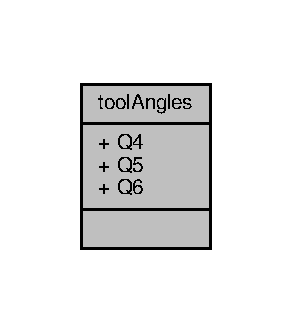
\includegraphics[width=140pt]{structtoolAngles__coll__graph}
\end{center}
\end{figure}
\subsection*{Öffentliche Attribute}
\begin{DoxyCompactItemize}
\item 
\hypertarget{structtoolAngles_a69ef685141e5c2d4e281c968328edb71}{double {\bfseries Q4}}\label{structtoolAngles_a69ef685141e5c2d4e281c968328edb71}

\item 
\hypertarget{structtoolAngles_acb61a7170bab38724e8c3cd75b7c7f3a}{double {\bfseries Q5}}\label{structtoolAngles_acb61a7170bab38724e8c3cd75b7c7f3a}

\item 
\hypertarget{structtoolAngles_a9075e6ee17f6548fdf073e366ec7a986}{double {\bfseries Q6}}\label{structtoolAngles_a9075e6ee17f6548fdf073e366ec7a986}

\end{DoxyCompactItemize}


Die Dokumentation für diese Struktur wurde erzeugt aufgrund der Datei\-:\begin{DoxyCompactItemize}
\item 
include/masterslave/Description\-Parameters.\-h\end{DoxyCompactItemize}

\hypertarget{structtoolDescriptionParameters}{\section{tool\-Description\-Parameters Strukturreferenz}
\label{structtoolDescriptionParameters}\index{tool\-Description\-Parameters@{tool\-Description\-Parameters}}
}


Zusammengehörigkeiten von tool\-Description\-Parameters\-:
\nopagebreak
\begin{figure}[H]
\begin{center}
\leavevmode
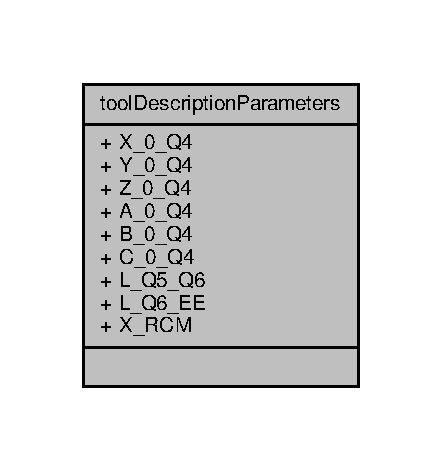
\includegraphics[width=212pt]{structtoolDescriptionParameters__coll__graph}
\end{center}
\end{figure}
\subsection*{Öffentliche Attribute}
\begin{DoxyCompactItemize}
\item 
\hypertarget{structtoolDescriptionParameters_a4e70eb885c9964a7d55947d2ebbc3941}{const double {\bfseries X\-\_\-0\-\_\-\-Q4}}\label{structtoolDescriptionParameters_a4e70eb885c9964a7d55947d2ebbc3941}

\item 
\hypertarget{structtoolDescriptionParameters_adb06f493573dbf08ae240d284160489b}{const double {\bfseries Y\-\_\-0\-\_\-\-Q4}}\label{structtoolDescriptionParameters_adb06f493573dbf08ae240d284160489b}

\item 
\hypertarget{structtoolDescriptionParameters_a2cf3044922cd2f75a3e02ad368908303}{const double {\bfseries Z\-\_\-0\-\_\-\-Q4}}\label{structtoolDescriptionParameters_a2cf3044922cd2f75a3e02ad368908303}

\item 
\hypertarget{structtoolDescriptionParameters_ab9694a03b68a2990c09544f8a332de0f}{const double {\bfseries A\-\_\-0\-\_\-\-Q4}}\label{structtoolDescriptionParameters_ab9694a03b68a2990c09544f8a332de0f}

\item 
\hypertarget{structtoolDescriptionParameters_a41be8e1344eb6f6fb6e4b2f3b8ac37cf}{const double {\bfseries B\-\_\-0\-\_\-\-Q4}}\label{structtoolDescriptionParameters_a41be8e1344eb6f6fb6e4b2f3b8ac37cf}

\item 
\hypertarget{structtoolDescriptionParameters_a2c30a06e314ce5ce2114d289569de757}{const double {\bfseries C\-\_\-0\-\_\-\-Q4}}\label{structtoolDescriptionParameters_a2c30a06e314ce5ce2114d289569de757}

\item 
\hypertarget{structtoolDescriptionParameters_a5fd9068ba1c97b74e4a25a002692729c}{const double {\bfseries L\-\_\-\-Q5\-\_\-\-Q6}}\label{structtoolDescriptionParameters_a5fd9068ba1c97b74e4a25a002692729c}

\item 
\hypertarget{structtoolDescriptionParameters_af7dd8266d4683dc4059736564b90fba3}{const double {\bfseries L\-\_\-\-Q6\-\_\-\-E\-E}}\label{structtoolDescriptionParameters_af7dd8266d4683dc4059736564b90fba3}

\item 
\hypertarget{structtoolDescriptionParameters_a79bb942eba1d071ff6adb0b2875d49e2}{const double {\bfseries X\-\_\-\-R\-C\-M}}\label{structtoolDescriptionParameters_a79bb942eba1d071ff6adb0b2875d49e2}

\end{DoxyCompactItemize}


Die Dokumentation für diese Struktur wurde erzeugt aufgrund der Datei\-:\begin{DoxyCompactItemize}
\item 
include/masterslave/Description\-Parameters.\-h\end{DoxyCompactItemize}

\hypertarget{structtoolMotorAngles}{\section{tool\-Motor\-Angles Strukturreferenz}
\label{structtoolMotorAngles}\index{tool\-Motor\-Angles@{tool\-Motor\-Angles}}
}


Zusammengehörigkeiten von tool\-Motor\-Angles\-:
\nopagebreak
\begin{figure}[H]
\begin{center}
\leavevmode
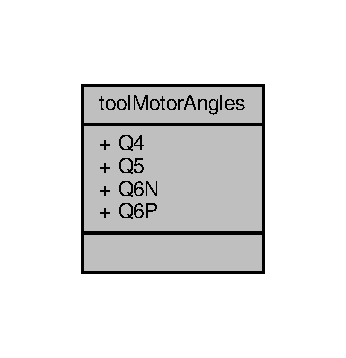
\includegraphics[width=166pt]{structtoolMotorAngles__coll__graph}
\end{center}
\end{figure}
\subsection*{Öffentliche Attribute}
\begin{DoxyCompactItemize}
\item 
\hypertarget{structtoolMotorAngles_a41e50f3d98f895173b2ebabea73350ac}{double {\bfseries Q4}}\label{structtoolMotorAngles_a41e50f3d98f895173b2ebabea73350ac}

\item 
\hypertarget{structtoolMotorAngles_a784134d746bab9b167b05fe3726f1926}{double {\bfseries Q5}}\label{structtoolMotorAngles_a784134d746bab9b167b05fe3726f1926}

\item 
\hypertarget{structtoolMotorAngles_a38d5906438b8617c8cbaae990b2ee626}{double {\bfseries Q6\-N}}\label{structtoolMotorAngles_a38d5906438b8617c8cbaae990b2ee626}

\item 
\hypertarget{structtoolMotorAngles_a42a9d5a3908822c03af99f9d17935041}{double {\bfseries Q6\-P}}\label{structtoolMotorAngles_a42a9d5a3908822c03af99f9d17935041}

\end{DoxyCompactItemize}


Die Dokumentation für diese Struktur wurde erzeugt aufgrund der Datei\-:\begin{DoxyCompactItemize}
\item 
include/masterslave/Description\-Parameters.\-h\end{DoxyCompactItemize}

\hypertarget{classTrajectoryGenerator}{\section{Trajectory\-Generator Klassenreferenz}
\label{classTrajectoryGenerator}\index{Trajectory\-Generator@{Trajectory\-Generator}}
}


Klasse zum Abfahren verschiedener Trajektorien zur quantitativen Bestimmung des Trokarpunktes.  




{\ttfamily \#include $<$Trajectory\-Generator.\-h$>$}



Zusammengehörigkeiten von Trajectory\-Generator\-:
\nopagebreak
\begin{figure}[H]
\begin{center}
\leavevmode
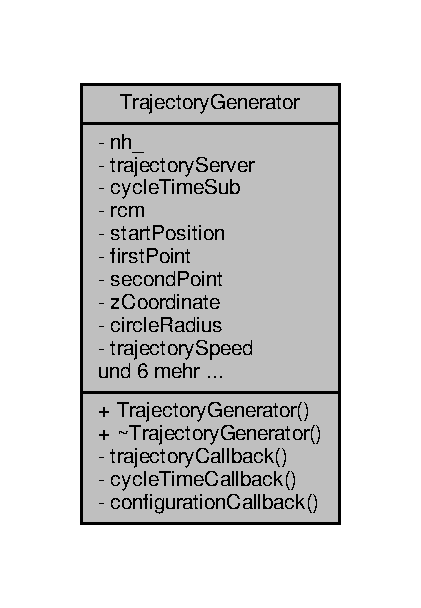
\includegraphics[width=202pt]{classTrajectoryGenerator__coll__graph}
\end{center}
\end{figure}
\subsection*{Öffentliche Methoden}
\begin{DoxyCompactItemize}
\item 
\hypertarget{classTrajectoryGenerator_af630ce00841ce126cbeca7dabec2b571}{{\bfseries Trajectory\-Generator} (ros\-::\-Node\-Handle \&nh)}\label{classTrajectoryGenerator_af630ce00841ce126cbeca7dabec2b571}

\end{DoxyCompactItemize}
\subsection*{Private Methoden}
\begin{DoxyCompactItemize}
\item 
bool \hyperlink{classTrajectoryGenerator_a78db2b3652839b0f16e959a859be78d1}{trajectory\-Callback} (masterslave\-::\-Manipulation\-::\-Request \&req, masterslave\-::\-Manipulation\-::\-Response \&resp)
\begin{DoxyCompactList}\small\item\em Callback der den aktuellen T\-C\-P bereitstellt und den neu bestimmten T\-C\-P als Antwort fordert. \end{DoxyCompactList}\item 
\hypertarget{classTrajectoryGenerator_a348c539543ae503b73b4f5380026a7cd}{void \hyperlink{classTrajectoryGenerator_a348c539543ae503b73b4f5380026a7cd}{cycle\-Time\-Callback} (const std\-\_\-msgs\-::\-Float64\-Const\-Ptr \&)}\label{classTrajectoryGenerator_a348c539543ae503b73b4f5380026a7cd}

\begin{DoxyCompactList}\small\item\em Bereitstellung der Zykluszeit über ein R\-O\-S-\/\-Topic. \end{DoxyCompactList}\item 
void \hyperlink{classTrajectoryGenerator_a542a3d9e6012e504a9bdd3e4d4415d97}{configuration\-Callback} (masterslave\-::\-Trajectory\-Generator\-Config \&config, uint32\-\_\-t level)
\begin{DoxyCompactList}\small\item\em Dynamic Reconfigure Callbackmethode. \end{DoxyCompactList}\end{DoxyCompactItemize}
\subsection*{Private Attribute}
\begin{DoxyCompactItemize}
\item 
\hypertarget{classTrajectoryGenerator_a1e215049f93f2b354d7d246ac8d070f2}{ros\-::\-Node\-Handle {\bfseries nh\-\_\-}}\label{classTrajectoryGenerator_a1e215049f93f2b354d7d246ac8d070f2}

\item 
\hypertarget{classTrajectoryGenerator_a33fc40f24dfab51390b800280dd8ce46}{ros\-::\-Service\-Server \hyperlink{classTrajectoryGenerator_a33fc40f24dfab51390b800280dd8ce46}{trajectory\-Server}}\label{classTrajectoryGenerator_a33fc40f24dfab51390b800280dd8ce46}

\begin{DoxyCompactList}\small\item\em Bereitstellung des Service Servers zur Manipulation des T\-C\-P. \end{DoxyCompactList}\item 
\hypertarget{classTrajectoryGenerator_a7250335d598f1d556b5e826dd206fbc8}{ros\-::\-Subscriber \hyperlink{classTrajectoryGenerator_a7250335d598f1d556b5e826dd206fbc8}{cycle\-Time\-Sub}}\label{classTrajectoryGenerator_a7250335d598f1d556b5e826dd206fbc8}

\begin{DoxyCompactList}\small\item\em Empfänger in R\-O\-S für die bereitgestellte Zykluszeit. \end{DoxyCompactList}\item 
\hypertarget{classTrajectoryGenerator_a676b24e0945d8a8623b3d9ca310b621b}{Eigen\-::\-Vector3d \hyperlink{classTrajectoryGenerator_a676b24e0945d8a8623b3d9ca310b621b}{rcm}}\label{classTrajectoryGenerator_a676b24e0945d8a8623b3d9ca310b621b}

\begin{DoxyCompactList}\small\item\em Position des Trokarpunktes im Weltkoordinatensystem. \end{DoxyCompactList}\item 
\hypertarget{classTrajectoryGenerator_a08c164f7f59ef59a7da96c96f0f60f73}{Eigen\-::\-Affine3d \hyperlink{classTrajectoryGenerator_a08c164f7f59ef59a7da96c96f0f60f73}{start\-Position}}\label{classTrajectoryGenerator_a08c164f7f59ef59a7da96c96f0f60f73}

\begin{DoxyCompactList}\small\item\em Aktuelle Startposition bzw. aktuelle T\-C\-P-\/\-Lage. \end{DoxyCompactList}\item 
\hypertarget{classTrajectoryGenerator_a608c44ff96e9d2504f35b8ff0233ec3b}{Eigen\-::\-Vector3d \hyperlink{classTrajectoryGenerator_a608c44ff96e9d2504f35b8ff0233ec3b}{first\-Point}}\label{classTrajectoryGenerator_a608c44ff96e9d2504f35b8ff0233ec3b}

\begin{DoxyCompactList}\small\item\em Erster Punkt der Trajektorie. \end{DoxyCompactList}\item 
\hypertarget{classTrajectoryGenerator_a1d6419470b689dd6cb23b0c7236fffd9}{Eigen\-::\-Vector3d \hyperlink{classTrajectoryGenerator_a1d6419470b689dd6cb23b0c7236fffd9}{second\-Point}}\label{classTrajectoryGenerator_a1d6419470b689dd6cb23b0c7236fffd9}

\begin{DoxyCompactList}\small\item\em Zweiter Punkt der Trajektorie. \end{DoxyCompactList}\item 
\hypertarget{classTrajectoryGenerator_abffbe637a297379a60c22f6efd53b8d9}{double \hyperlink{classTrajectoryGenerator_abffbe637a297379a60c22f6efd53b8d9}{z\-Coordinate}}\label{classTrajectoryGenerator_abffbe637a297379a60c22f6efd53b8d9}

\begin{DoxyCompactList}\small\item\em z-\/\-Koordinate des Kreismittelpunktes \end{DoxyCompactList}\item 
\hypertarget{classTrajectoryGenerator_ac02b6a2df43dc5706507835ad5cb84d8}{double \hyperlink{classTrajectoryGenerator_ac02b6a2df43dc5706507835ad5cb84d8}{circle\-Radius}}\label{classTrajectoryGenerator_ac02b6a2df43dc5706507835ad5cb84d8}

\begin{DoxyCompactList}\small\item\em Radius der Kreistrajectorie. \end{DoxyCompactList}\item 
\hypertarget{classTrajectoryGenerator_a908a13ec9428ff58ea9c4622b3845337}{double \hyperlink{classTrajectoryGenerator_a908a13ec9428ff58ea9c4622b3845337}{trajectory\-Speed}}\label{classTrajectoryGenerator_a908a13ec9428ff58ea9c4622b3845337}

\begin{DoxyCompactList}\small\item\em Durchschnittliche Trajektoriengeschwindigkeit in \mbox{[}mm/s\mbox{]}. \end{DoxyCompactList}\item 
\hypertarget{classTrajectoryGenerator_aac65fb524447f9d1e77fb52bfcf70307}{double \hyperlink{classTrajectoryGenerator_aac65fb524447f9d1e77fb52bfcf70307}{cycle\-Time}}\label{classTrajectoryGenerator_aac65fb524447f9d1e77fb52bfcf70307}

\begin{DoxyCompactList}\small\item\em Zykluszeit. \end{DoxyCompactList}\item 
\hypertarget{classTrajectoryGenerator_acebd9fea08097528dbf013d327c39f7c}{bool \hyperlink{classTrajectoryGenerator_acebd9fea08097528dbf013d327c39f7c}{start} \{false\}}\label{classTrajectoryGenerator_acebd9fea08097528dbf013d327c39f7c}

\begin{DoxyCompactList}\small\item\em Startflag, die über Dynamic Reconfigure übertragen wird. \end{DoxyCompactList}\item 
\hypertarget{classTrajectoryGenerator_a4692340647fc11a62aec0cd32194cb45}{bool \hyperlink{classTrajectoryGenerator_a4692340647fc11a62aec0cd32194cb45}{rcm\-Position\-There} \{false\}}\label{classTrajectoryGenerator_a4692340647fc11a62aec0cd32194cb45}

\begin{DoxyCompactList}\small\item\em Flag, ob der R\-C\-M empfangen wurde. \end{DoxyCompactList}\item 
\hypertarget{classTrajectoryGenerator_ab32e4cd8abfe7740a3f7113fbff506b7}{const double {\bfseries M\-M\-\_\-\-T\-O\-\_\-\-M} \{0.\-001\}}\label{classTrajectoryGenerator_ab32e4cd8abfe7740a3f7113fbff506b7}

\item 
std\-::unique\-\_\-ptr$<$ \hyperlink{classITrajectory}{I\-Trajectory} $>$ \hyperlink{classTrajectoryGenerator_ad945c2000eeab78342a67d627886e211}{trajectory\-Gen}
\begin{DoxyCompactList}\small\item\em Zeiger auf das Trajectorienobjekt. \end{DoxyCompactList}\item 
\hypertarget{classTrajectoryGenerator_a3ac417739c130895c6fbdea8b751d496}{\hyperlink{TrajectoryGenerator_8h_ab7e9971a19ca76371c40959c478f6618}{T\-R\-A\-J\-E\-C\-T\-O\-R\-Y\-\_\-\-S\-T\-A\-T\-E} \hyperlink{classTrajectoryGenerator_a3ac417739c130895c6fbdea8b751d496}{state} \{N\-O\-\_\-\-S\-T\-A\-T\-E\}}\label{classTrajectoryGenerator_a3ac417739c130895c6fbdea8b751d496}

\begin{DoxyCompactList}\small\item\em Aktuell gewünschte Trajektorienform. \end{DoxyCompactList}\end{DoxyCompactItemize}


\subsection{Ausführliche Beschreibung}
Klasse zum Abfahren verschiedener Trajektorien zur quantitativen Bestimmung des Trokarpunktes. 

\begin{DoxyAuthor}{Autor}
Fabian Baier 
\end{DoxyAuthor}
\begin{DoxyDate}{Datum}
20.\-03.\-2016 
\end{DoxyDate}


\subsection{Dokumentation der Elementfunktionen}
\hypertarget{classTrajectoryGenerator_a542a3d9e6012e504a9bdd3e4d4415d97}{\index{Trajectory\-Generator@{Trajectory\-Generator}!configuration\-Callback@{configuration\-Callback}}
\index{configuration\-Callback@{configuration\-Callback}!TrajectoryGenerator@{Trajectory\-Generator}}
\subsubsection[{configuration\-Callback}]{\setlength{\rightskip}{0pt plus 5cm}Trajectory\-Generator\-::configuration\-Callback (
\begin{DoxyParamCaption}
\item[{masterslave\-::\-Trajectory\-Generator\-Config \&}]{config, }
\item[{uint32\-\_\-t}]{level}
\end{DoxyParamCaption}
)\hspace{0.3cm}{\ttfamily [private]}}}\label{classTrajectoryGenerator_a542a3d9e6012e504a9bdd3e4d4415d97}


Dynamic Reconfigure Callbackmethode. 


\begin{DoxyParams}{Parameter}
{\em config} & Dynamic Reconfigure Configuration \\
\hline
{\em level} & Bitmaske \\
\hline
\end{DoxyParams}
\begin{DoxySeeAlso}{Siehe auch}
Trajectory\-Generator.\-cfg 
\end{DoxySeeAlso}
\hypertarget{classTrajectoryGenerator_a78db2b3652839b0f16e959a859be78d1}{\index{Trajectory\-Generator@{Trajectory\-Generator}!trajectory\-Callback@{trajectory\-Callback}}
\index{trajectory\-Callback@{trajectory\-Callback}!TrajectoryGenerator@{Trajectory\-Generator}}
\subsubsection[{trajectory\-Callback}]{\setlength{\rightskip}{0pt plus 5cm}Trajectory\-Generator\-::trajectory\-Callback (
\begin{DoxyParamCaption}
\item[{masterslave\-::\-Manipulation\-::\-Request \&}]{req, }
\item[{masterslave\-::\-Manipulation\-::\-Response \&}]{resp}
\end{DoxyParamCaption}
)\hspace{0.3cm}{\ttfamily [private]}}}\label{classTrajectoryGenerator_a78db2b3652839b0f16e959a859be78d1}


Callback der den aktuellen T\-C\-P bereitstellt und den neu bestimmten T\-C\-P als Antwort fordert. 


\begin{DoxyParams}{Parameter}
{\em req} & T\-C\-P vor der Manipulation \\
\hline
{\em resp} & T\-C\-P nach der Manipulation \\
\hline
\end{DoxyParams}
\begin{DoxyReturn}{Rückgabe}
Flag, ob der Serviceaufruf erfolgreich war 
\end{DoxyReturn}


\subsection{Dokumentation der Datenelemente}
\hypertarget{classTrajectoryGenerator_ad945c2000eeab78342a67d627886e211}{\index{Trajectory\-Generator@{Trajectory\-Generator}!trajectory\-Gen@{trajectory\-Gen}}
\index{trajectory\-Gen@{trajectory\-Gen}!TrajectoryGenerator@{Trajectory\-Generator}}
\subsubsection[{trajectory\-Gen}]{\setlength{\rightskip}{0pt plus 5cm}Trajectory\-Generator\-::trajectory\-Gen\hspace{0.3cm}{\ttfamily [private]}}}\label{classTrajectoryGenerator_ad945c2000eeab78342a67d627886e211}


Zeiger auf das Trajectorienobjekt. 

\begin{DoxySeeAlso}{Siehe auch}
\hyperlink{classITrajectory}{I\-Trajectory} 
\end{DoxySeeAlso}


Die Dokumentation für diese Klasse wurde erzeugt aufgrund der Datei\-:\begin{DoxyCompactItemize}
\item 
include/masterslave/manipulation/\hyperlink{TrajectoryGenerator_8h}{Trajectory\-Generator.\-h}\end{DoxyCompactItemize}

\chapter{Datei-\/\-Dokumentation}
\hypertarget{BoundingBox_8h}{\section{include/masterslave/commander/\-Bounding\-Box.h-\/\-Dateireferenz}
\label{BoundingBox_8h}\index{include/masterslave/commander/\-Bounding\-Box.\-h@{include/masterslave/commander/\-Bounding\-Box.\-h}}
}
{\ttfamily \#include $<$Eigen/\-Dense$>$}\\*
{\ttfamily \#include $<$ros/ros.\-h$>$}\\*
{\ttfamily \#include $<$geometry\-\_\-msgs/\-Point.\-h$>$}\\*
{\ttfamily \#include $<$tf\-\_\-conversions/tf\-\_\-eigen.\-h$>$}\\*
{\ttfamily \#include $<$eigen\-\_\-conversions/eigen\-\_\-msg.\-h$>$}\\*
Include-\/\-Abhängigkeitsdiagramm für Bounding\-Box.\-h\-:
\nopagebreak
\begin{figure}[H]
\begin{center}
\leavevmode
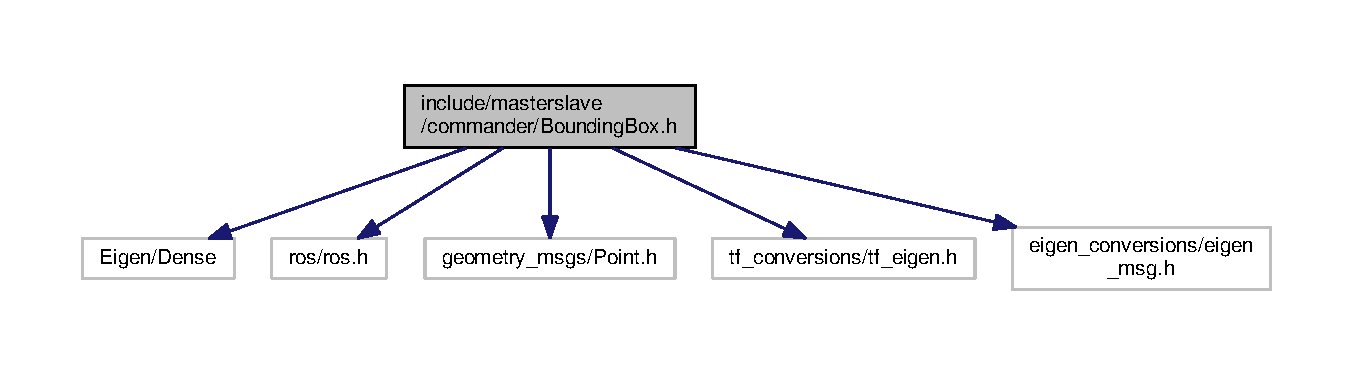
\includegraphics[width=350pt]{BoundingBox_8h__incl}
\end{center}
\end{figure}
Dieser Graph zeigt, welche Datei direkt oder indirekt diese Datei enthält\-:
\nopagebreak
\begin{figure}[H]
\begin{center}
\leavevmode
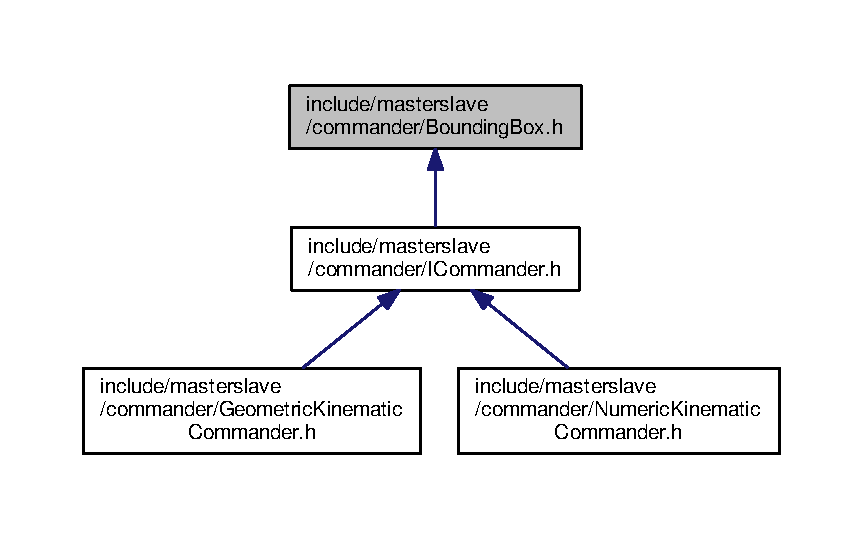
\includegraphics[width=350pt]{BoundingBox_8h__dep__incl}
\end{center}
\end{figure}
\subsection*{Klassen}
\begin{DoxyCompactItemize}
\item 
class \hyperlink{classBoundingBox}{Bounding\-Box}
\begin{DoxyCompactList}\small\item\em Arbeitsraumbegrenzung in Form eines Quaders. \end{DoxyCompactList}\end{DoxyCompactItemize}

\hypertarget{GeometricKinematicCommander_8h}{\section{include/masterslave/commander/\-Geometric\-Kinematic\-Commander.h-\/\-Dateireferenz}
\label{GeometricKinematicCommander_8h}\index{include/masterslave/commander/\-Geometric\-Kinematic\-Commander.\-h@{include/masterslave/commander/\-Geometric\-Kinematic\-Commander.\-h}}
}
{\ttfamily \#include \char`\"{}I\-Commander.\-h\char`\"{}}\\*
{\ttfamily \#include \char`\"{}masterslave/kinematic/\-Geometric\-Kinematic.\-h\char`\"{}}\\*
{\ttfamily \#include \char`\"{}ros/ros.\-h\char`\"{}}\\*
{\ttfamily \#include $<$tf/tf.\-h$>$}\\*
{\ttfamily \#include $<$tf\-\_\-conversions/tf\-\_\-eigen.\-h$>$}\\*
{\ttfamily \#include $<$eigen\-\_\-conversions/eigen\-\_\-msg.\-h$>$}\\*
{\ttfamily \#include $<$tf/transform\-\_\-listener.\-h$>$}\\*
Include-\/\-Abhängigkeitsdiagramm für Geometric\-Kinematic\-Commander.\-h\-:
\nopagebreak
\begin{figure}[H]
\begin{center}
\leavevmode
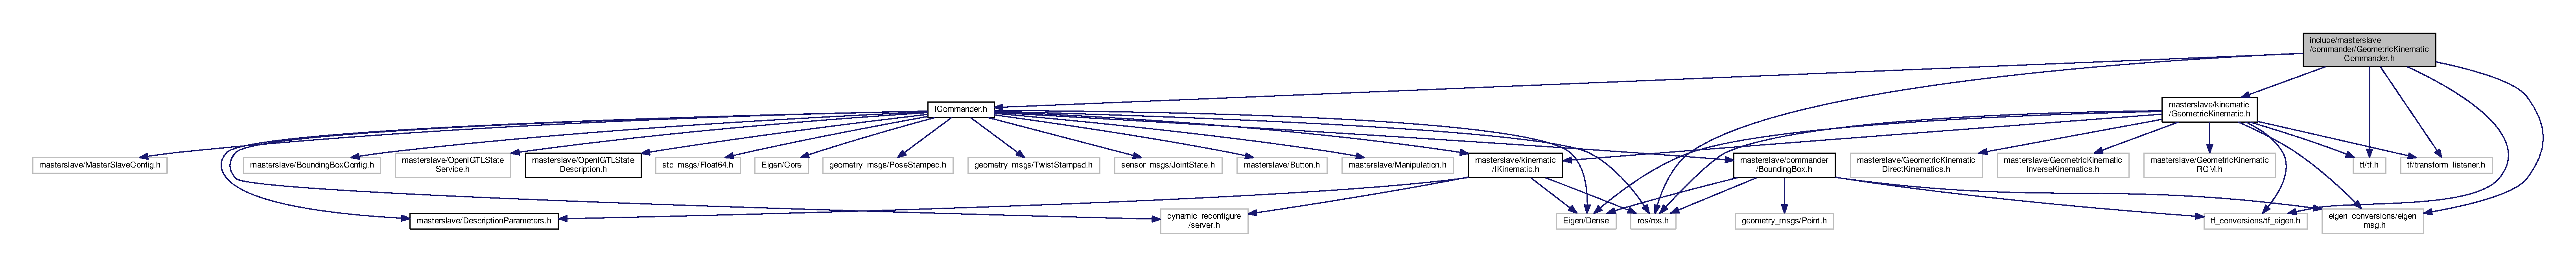
\includegraphics[width=350pt]{GeometricKinematicCommander_8h__incl}
\end{center}
\end{figure}
\subsection*{Klassen}
\begin{DoxyCompactItemize}
\item 
class \hyperlink{classGeometricKinematicCommander}{Geometric\-Kinematic\-Commander}
\begin{DoxyCompactList}\small\item\em Klasse, die sich um die R\-O\-S-\/\-Kommunikation für die geometrisch bestimmte Kinematik kümmert. \end{DoxyCompactList}\end{DoxyCompactItemize}

\hypertarget{ICommander_8h}{\section{include/masterslave/commander/\-I\-Commander.h-\/\-Dateireferenz}
\label{ICommander_8h}\index{include/masterslave/commander/\-I\-Commander.\-h@{include/masterslave/commander/\-I\-Commander.\-h}}
}
{\ttfamily \#include $<$ros/ros.\-h$>$}\\*
{\ttfamily \#include $<$std\-\_\-msgs/\-Float64.\-h$>$}\\*
{\ttfamily \#include \char`\"{}Eigen/\-Dense\char`\"{}}\\*
{\ttfamily \#include \char`\"{}Eigen/\-Core\char`\"{}}\\*
{\ttfamily \#include \char`\"{}masterslave/\-Description\-Parameters.\-h\char`\"{}}\\*
{\ttfamily \#include \char`\"{}masterslave/kinematic/\-I\-Kinematic.\-h\char`\"{}}\\*
{\ttfamily \#include \char`\"{}masterslave/commander/\-Bounding\-Box.\-h\char`\"{}}\\*
{\ttfamily \#include \char`\"{}geometry\-\_\-msgs/\-Pose\-Stamped.\-h\char`\"{}}\\*
{\ttfamily \#include \char`\"{}geometry\-\_\-msgs/\-Twist\-Stamped.\-h\char`\"{}}\\*
{\ttfamily \#include \char`\"{}sensor\-\_\-msgs/\-Joint\-State.\-h\char`\"{}}\\*
{\ttfamily \#include \char`\"{}masterslave/\-Button.\-h\char`\"{}}\\*
{\ttfamily \#include \char`\"{}masterslave/\-Manipulation.\-h\char`\"{}}\\*
{\ttfamily \#include $<$dynamic\-\_\-reconfigure/server.\-h$>$}\\*
{\ttfamily \#include $<$masterslave/\-Master\-Slave\-Config.\-h$>$}\\*
{\ttfamily \#include $<$masterslave/\-Bounding\-Box\-Config.\-h$>$}\\*
{\ttfamily \#include \char`\"{}masterslave/\-Open\-I\-G\-T\-L\-State\-Service.\-h\char`\"{}}\\*
{\ttfamily \#include \char`\"{}masterslave/\-Open\-I\-G\-T\-L\-State\-Description.\-h\char`\"{}}\\*
Include-\/\-Abhängigkeitsdiagramm für I\-Commander.\-h\-:
\nopagebreak
\begin{figure}[H]
\begin{center}
\leavevmode
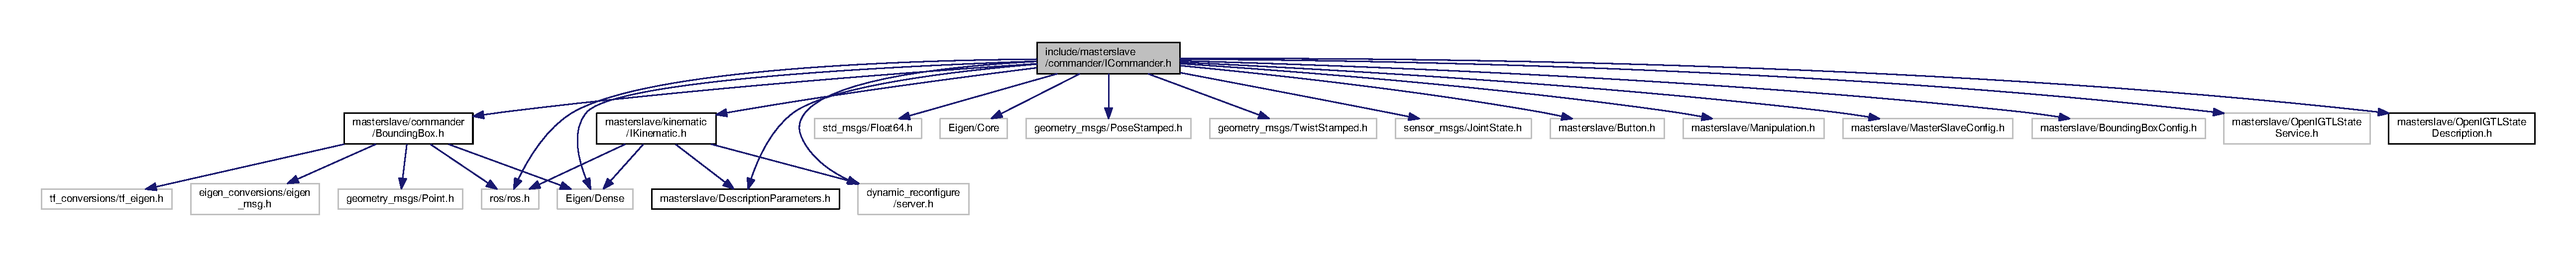
\includegraphics[width=350pt]{ICommander_8h__incl}
\end{center}
\end{figure}
Dieser Graph zeigt, welche Datei direkt oder indirekt diese Datei enthält\-:
\nopagebreak
\begin{figure}[H]
\begin{center}
\leavevmode
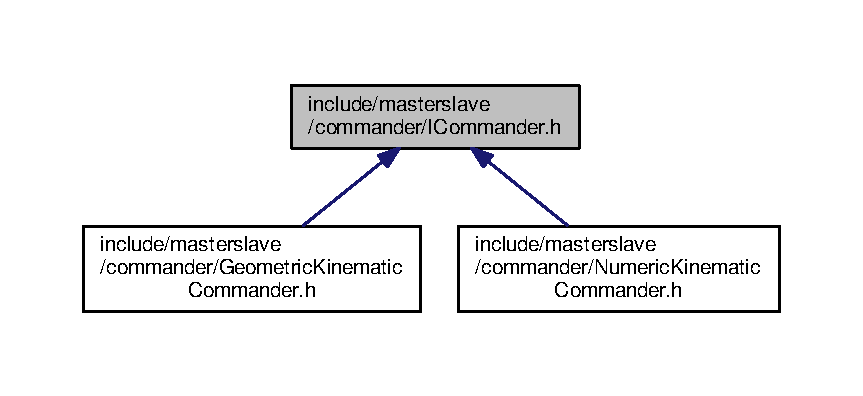
\includegraphics[width=350pt]{ICommander_8h__dep__incl}
\end{center}
\end{figure}
\subsection*{Klassen}
\begin{DoxyCompactItemize}
\item 
class \hyperlink{classICommander}{I\-Commander}
\begin{DoxyCompactList}\small\item\em Abstrakte Basisklasse zur Ansteuerung der beiden Kinematikmodelle über R\-O\-S. \end{DoxyCompactList}\end{DoxyCompactItemize}

\hypertarget{NumericKinematicCommander_8h}{\section{include/masterslave/commander/\-Numeric\-Kinematic\-Commander.h-\/\-Dateireferenz}
\label{NumericKinematicCommander_8h}\index{include/masterslave/commander/\-Numeric\-Kinematic\-Commander.\-h@{include/masterslave/commander/\-Numeric\-Kinematic\-Commander.\-h}}
}
{\ttfamily \#include $<$array$>$}\\*
{\ttfamily \#include \char`\"{}I\-Commander.\-h\char`\"{}}\\*
{\ttfamily \#include \char`\"{}ros/ros.\-h\char`\"{}}\\*
{\ttfamily \#include \char`\"{}sensor\-\_\-msgs/\-Joint\-State.\-h\char`\"{}}\\*
{\ttfamily \#include \char`\"{}geometry\-\_\-msgs/\-Pose\-Stamped.\-h\char`\"{}}\\*
{\ttfamily \#include \char`\"{}masterslave/\-Numeric\-Kinematic\-R\-C\-M.\-h\char`\"{}}\\*
{\ttfamily \#include \char`\"{}masterslave/\-Numeric\-Kinematic\-Direct\-Kinematics.\-h\char`\"{}}\\*
{\ttfamily \#include \char`\"{}masterslave/\-Numeric\-Kinematic\-Inverse\-Kinematics.\-h\char`\"{}}\\*
{\ttfamily \#include $<$tf/tf.\-h$>$}\\*
{\ttfamily \#include $<$tf\-\_\-conversions/tf\-\_\-eigen.\-h$>$}\\*
{\ttfamily \#include $<$eigen\-\_\-conversions/eigen\-\_\-msg.\-h$>$}\\*
{\ttfamily \#include $<$tf/transform\-\_\-listener.\-h$>$}\\*
Include-\/\-Abhängigkeitsdiagramm für Numeric\-Kinematic\-Commander.\-h\-:
\nopagebreak
\begin{figure}[H]
\begin{center}
\leavevmode
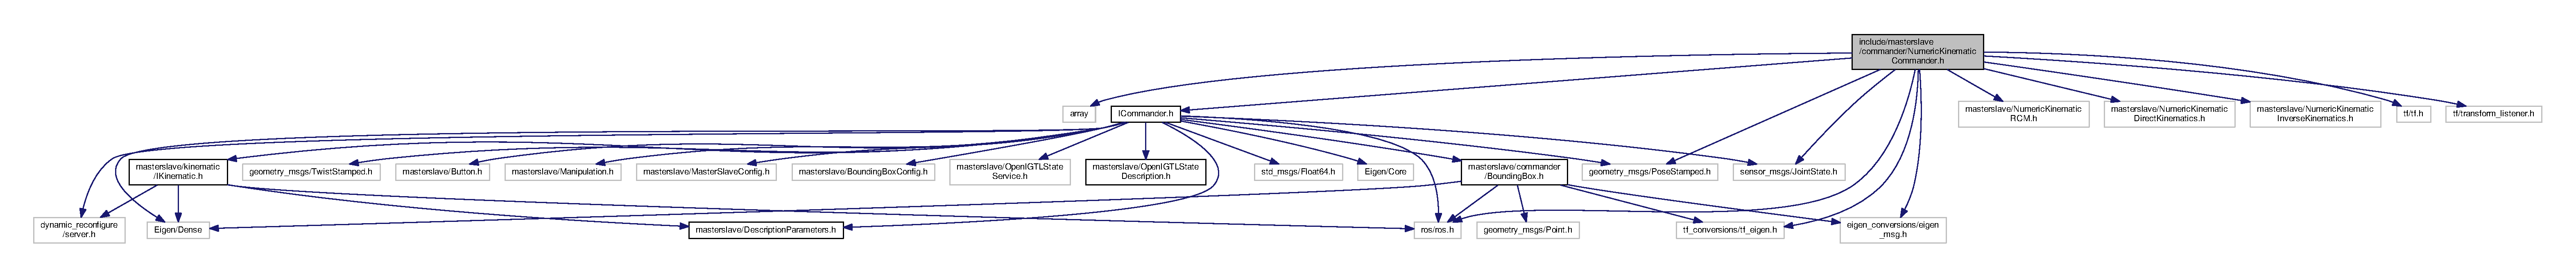
\includegraphics[width=350pt]{NumericKinematicCommander_8h__incl}
\end{center}
\end{figure}
\subsection*{Klassen}
\begin{DoxyCompactItemize}
\item 
class \hyperlink{classNumericKinematicCommander}{Numeric\-Kinematic\-Commander}
\begin{DoxyCompactList}\small\item\em Klasse, die sich um die R\-O\-S-\/\-Kommunikation für die numerisch bestimmte Kinematik kümmert. \end{DoxyCompactList}\end{DoxyCompactItemize}

\hypertarget{ControlDevice_8h}{\section{include/masterslave/\-Control\-Device.h-\/\-Dateireferenz}
\label{ControlDevice_8h}\index{include/masterslave/\-Control\-Device.\-h@{include/masterslave/\-Control\-Device.\-h}}
}
{\ttfamily \#include $<$ros/ros.\-h$>$}\\*
{\ttfamily \#include \char`\"{}geometry\-\_\-msgs/\-Twist\-Stamped.\-h\char`\"{}}\\*
{\ttfamily \#include \char`\"{}masterslave/\-Button.\-h\char`\"{}}\\*
{\ttfamily \#include \char`\"{}sensor\-\_\-msgs/\-Joy.\-h\char`\"{}}\\*
{\ttfamily \#include $<$string$>$}\\*
{\ttfamily \#include $<$vector$>$}\\*
{\ttfamily \#include $<$map$>$}\\*
{\ttfamily \#include $<$algorithm$>$}\\*
{\ttfamily \#include $<$sstream$>$}\\*
{\ttfamily \#include $<$dynamic\-\_\-reconfigure/server.\-h$>$}\\*
{\ttfamily \#include $<$masterslave/\-Control\-Device\-Config.\-h$>$}\\*
Include-\/\-Abhängigkeitsdiagramm für Control\-Device.\-h\-:
\nopagebreak
\begin{figure}[H]
\begin{center}
\leavevmode
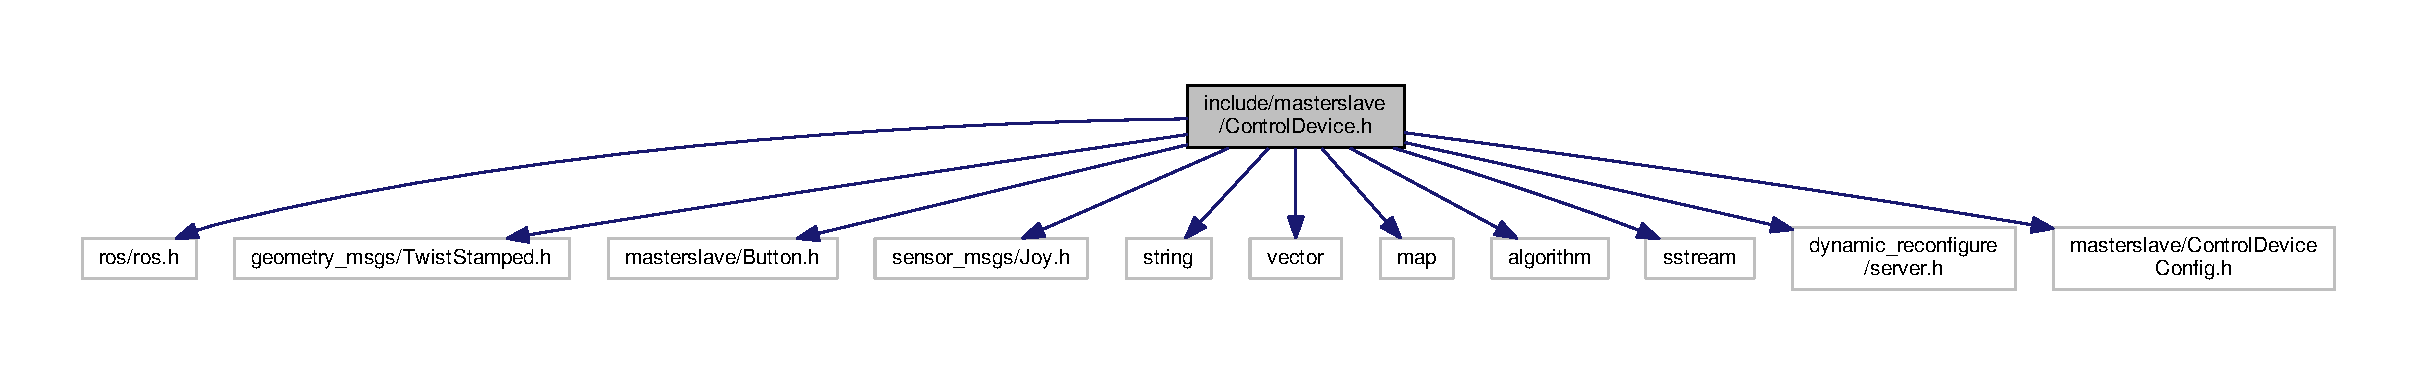
\includegraphics[width=350pt]{ControlDevice_8h__incl}
\end{center}
\end{figure}
\subsection*{Klassen}
\begin{DoxyCompactItemize}
\item 
class \hyperlink{classControlDevice}{Control\-Device}
\begin{DoxyCompactList}\small\item\em Klasse zur Ansteuerung und Verwaltung verschiedener Low\-Level-\/\-Eingabegeräte, wie Game\-Pads oder dem Space\-Navigator. \end{DoxyCompactList}\end{DoxyCompactItemize}

\hypertarget{GeometricKinematic_8h}{\section{include/masterslave/kinematic/\-Geometric\-Kinematic.h-\/\-Dateireferenz}
\label{GeometricKinematic_8h}\index{include/masterslave/kinematic/\-Geometric\-Kinematic.\-h@{include/masterslave/kinematic/\-Geometric\-Kinematic.\-h}}
}
{\ttfamily \#include \char`\"{}I\-Kinematic.\-h\char`\"{}}\\*
{\ttfamily \#include \char`\"{}Eigen/\-Dense\char`\"{}}\\*
{\ttfamily \#include \char`\"{}ros/ros.\-h\char`\"{}}\\*
{\ttfamily \#include \char`\"{}masterslave/\-Geometric\-Kinematic\-Direct\-Kinematics.\-h\char`\"{}}\\*
{\ttfamily \#include \char`\"{}masterslave/\-Geometric\-Kinematic\-Inverse\-Kinematics.\-h\char`\"{}}\\*
{\ttfamily \#include \char`\"{}masterslave/\-Geometric\-Kinematic\-R\-C\-M.\-h\char`\"{}}\\*
{\ttfamily \#include $<$tf/tf.\-h$>$}\\*
{\ttfamily \#include $<$tf\-\_\-conversions/tf\-\_\-eigen.\-h$>$}\\*
{\ttfamily \#include $<$eigen\-\_\-conversions/eigen\-\_\-msg.\-h$>$}\\*
{\ttfamily \#include $<$tf/transform\-\_\-listener.\-h$>$}\\*
Include-\/\-Abhängigkeitsdiagramm für Geometric\-Kinematic.\-h\-:
\nopagebreak
\begin{figure}[H]
\begin{center}
\leavevmode
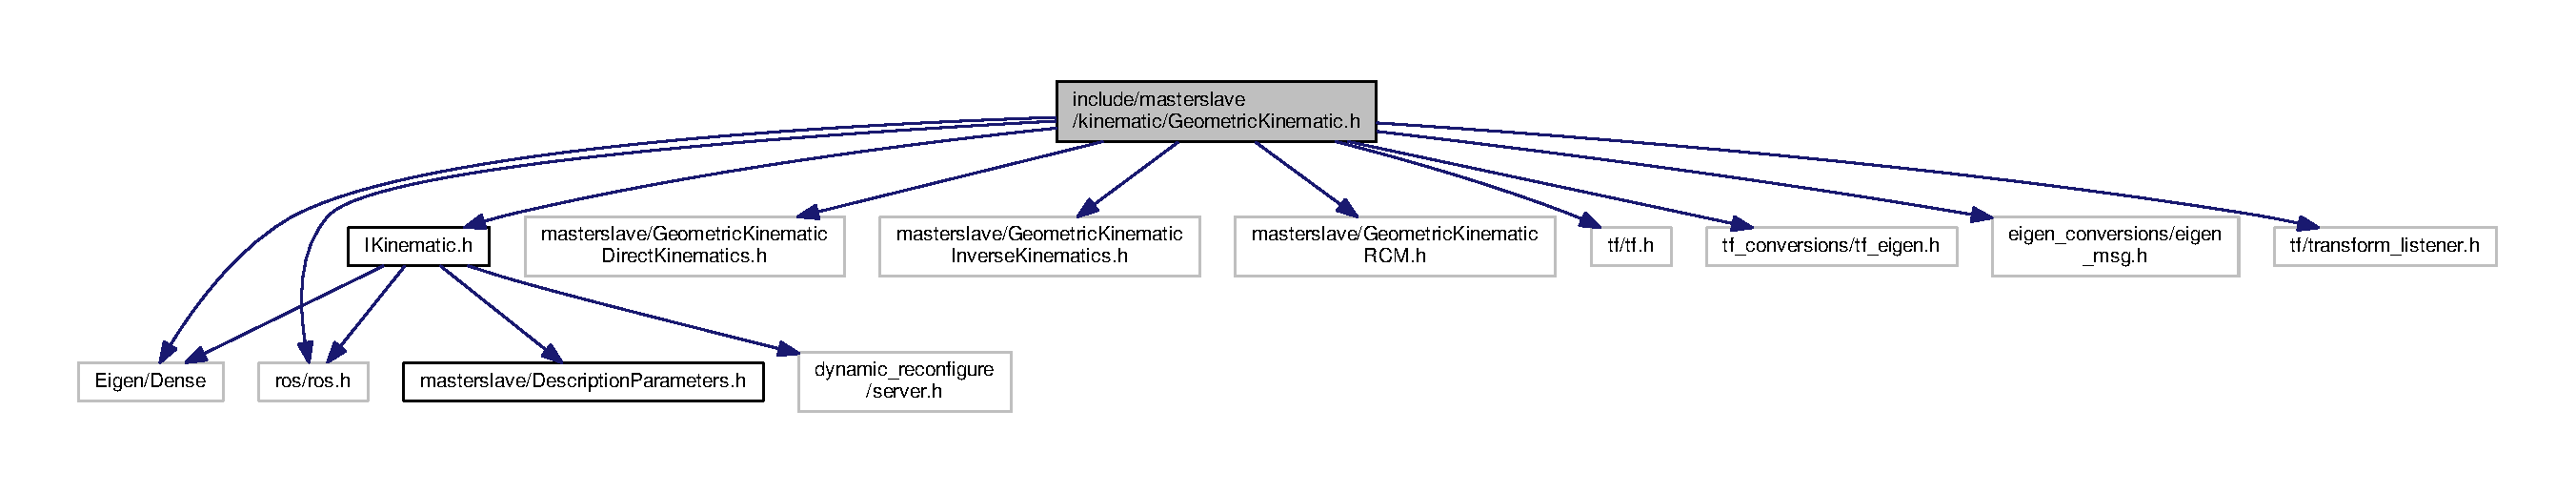
\includegraphics[width=350pt]{GeometricKinematic_8h__incl}
\end{center}
\end{figure}
Dieser Graph zeigt, welche Datei direkt oder indirekt diese Datei enthält\-:
\nopagebreak
\begin{figure}[H]
\begin{center}
\leavevmode
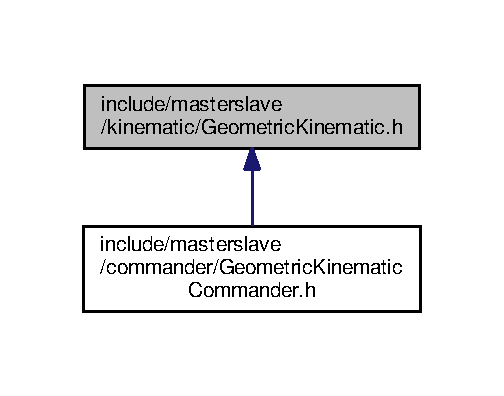
\includegraphics[width=242pt]{GeometricKinematic_8h__dep__incl}
\end{center}
\end{figure}
\subsection*{Klassen}
\begin{DoxyCompactItemize}
\item 
class \hyperlink{classGeometricKinematic}{Geometric\-Kinematic}
\begin{DoxyCompactList}\small\item\em Eine Klasse zur Berechnung der Kinematik des Werkzeuges und der Endeffektorlage des L\-B\-R iiwa. \end{DoxyCompactList}\end{DoxyCompactItemize}

\hypertarget{IKinematic_8h}{\section{include/masterslave/kinematic/\-I\-Kinematic.h-\/\-Dateireferenz}
\label{IKinematic_8h}\index{include/masterslave/kinematic/\-I\-Kinematic.\-h@{include/masterslave/kinematic/\-I\-Kinematic.\-h}}
}
{\ttfamily \#include \char`\"{}Eigen/\-Dense\char`\"{}}\\*
{\ttfamily \#include \char`\"{}ros/ros.\-h\char`\"{}}\\*
{\ttfamily \#include \char`\"{}masterslave/\-Description\-Parameters.\-h\char`\"{}}\\*
{\ttfamily \#include $<$dynamic\-\_\-reconfigure/server.\-h$>$}\\*
Include-\/\-Abhängigkeitsdiagramm für I\-Kinematic.\-h\-:
\nopagebreak
\begin{figure}[H]
\begin{center}
\leavevmode
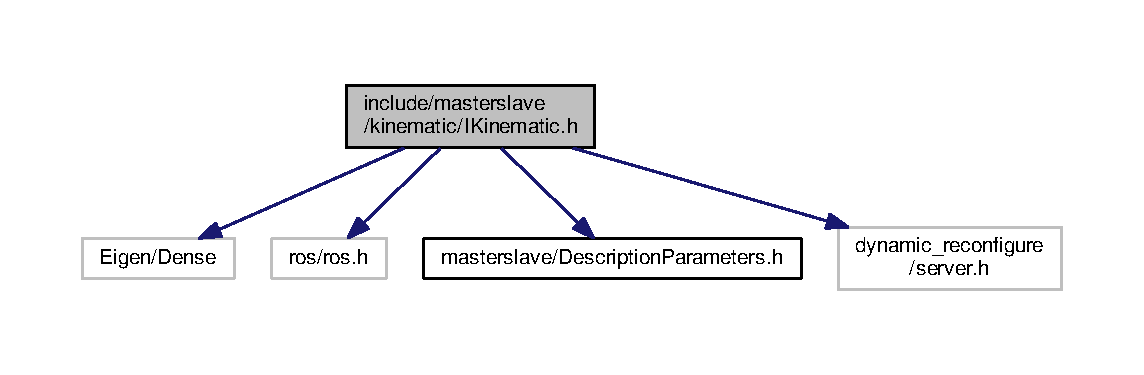
\includegraphics[width=350pt]{IKinematic_8h__incl}
\end{center}
\end{figure}
Dieser Graph zeigt, welche Datei direkt oder indirekt diese Datei enthält\-:
\nopagebreak
\begin{figure}[H]
\begin{center}
\leavevmode
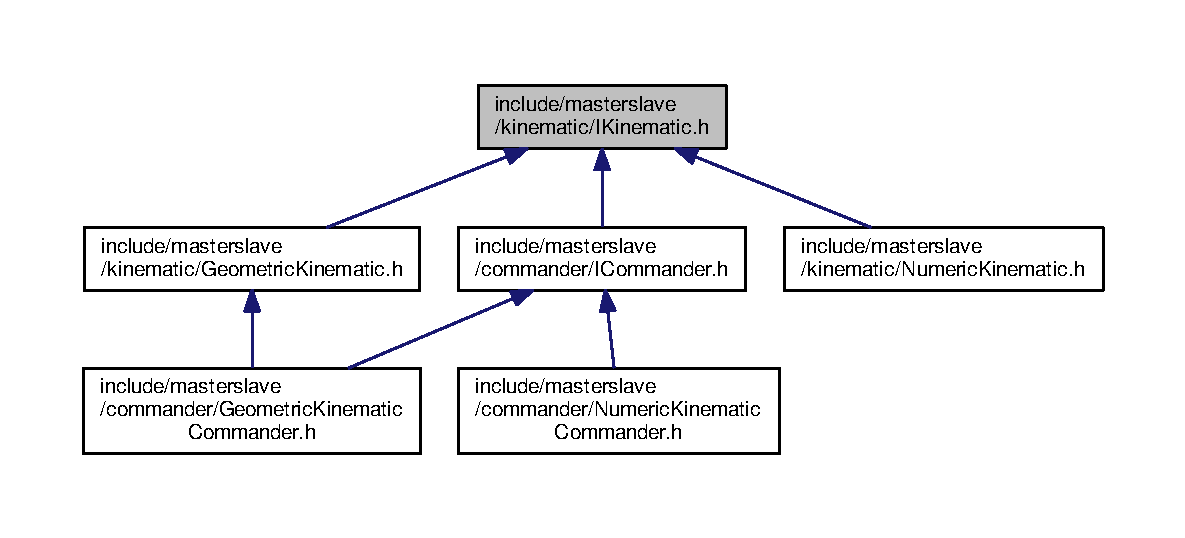
\includegraphics[width=350pt]{IKinematic_8h__dep__incl}
\end{center}
\end{figure}
\subsection*{Klassen}
\begin{DoxyCompactItemize}
\item 
class \hyperlink{classIKinematic}{I\-Kinematic}
\begin{DoxyCompactList}\small\item\em Abstrakte Basisklasse für die Kinematikberechnung. \end{DoxyCompactList}\end{DoxyCompactItemize}

\hypertarget{NumericKinematic_8h}{\section{include/masterslave/kinematic/\-Numeric\-Kinematic.h-\/\-Dateireferenz}
\label{NumericKinematic_8h}\index{include/masterslave/kinematic/\-Numeric\-Kinematic.\-h@{include/masterslave/kinematic/\-Numeric\-Kinematic.\-h}}
}
{\ttfamily \#include \char`\"{}I\-Kinematic.\-h\char`\"{}}\\*
{\ttfamily \#include $<$eigen3/\-Eigen/\-Core$>$}\\*
{\ttfamily \#include \char`\"{}ros/ros.\-h\char`\"{}}\\*
{\ttfamily \#include \char`\"{}masterslave/\-Numeric\-Kinematic\-R\-C\-M.\-h\char`\"{}}\\*
{\ttfamily \#include \char`\"{}masterslave/\-Numeric\-Kinematic\-Direct\-Kinematics.\-h\char`\"{}}\\*
{\ttfamily \#include \char`\"{}masterslave/\-Numeric\-Kinematic\-Inverse\-Kinematics.\-h\char`\"{}}\\*
{\ttfamily \#include \char`\"{}masterslave/\-Numeric\-Kinematic\-Config.\-h\char`\"{}}\\*
{\ttfamily \#include $<$tf/tf.\-h$>$}\\*
{\ttfamily \#include $<$tf\-\_\-conversions/tf\-\_\-eigen.\-h$>$}\\*
{\ttfamily \#include $<$eigen\-\_\-conversions/eigen\-\_\-msg.\-h$>$}\\*
{\ttfamily \#include $<$tf/transform\-\_\-listener.\-h$>$}\\*
{\ttfamily \#include $<$std\-\_\-msgs/\-Float64.\-h$>$}\\*
{\ttfamily \#include \char`\"{}eiquadprog.\-hpp\char`\"{}}\\*
Include-\/\-Abhängigkeitsdiagramm für Numeric\-Kinematic.\-h\-:
\nopagebreak
\begin{figure}[H]
\begin{center}
\leavevmode
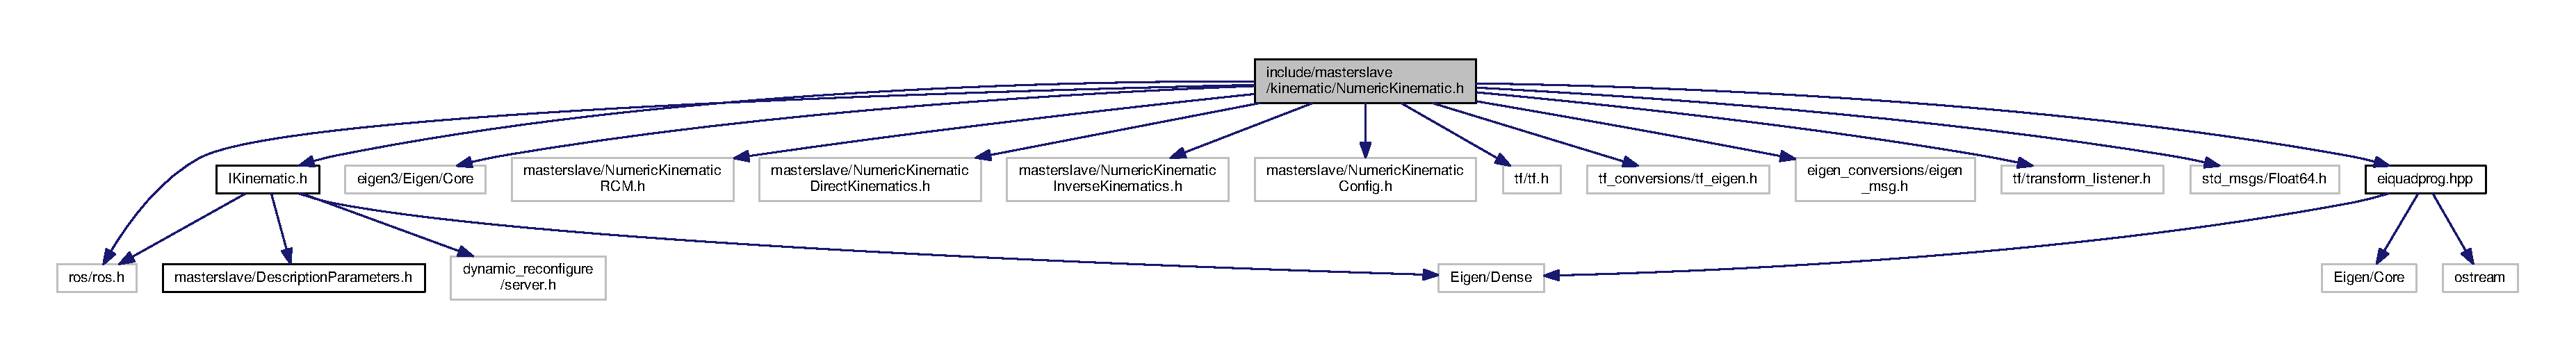
\includegraphics[width=350pt]{NumericKinematic_8h__incl}
\end{center}
\end{figure}
\subsection*{Klassen}
\begin{DoxyCompactItemize}
\item 
class \hyperlink{classNumericKinematic}{Numeric\-Kinematic}
\begin{DoxyCompactList}\small\item\em Klasse zur Berechnung der Kinematiken des Gesamtsystems mit 10 Achsen. Die inverse Kinematik wird numerisch mittels eines Least-\/\-Square-\/\-Problems gelöst Die Klasse berechnet die direkte und inverse Kinematik eines Gesamtsystems bestehend aus L\-B\-R iiwa und dem Laparoskop. Es besitzt insgesamt 10 Achsen, da der Trokarpunkt eingehalten werden muss, bleibt noch eine Redundanz mit Dimension 2 zur Optimierung der Gelenkwinkelkonfiguration. Diese können mit verschiedenen Optimierungskriterien, wie Singularitätsvermeidung, Kollisionsvermeidung, Geschwindigkeits-\/ und Beschleunigungsminimierung, sowie einer Winkelwächterfunktion parametriert werden Zum Lösen wird der Algorithmus aus Quad\-Prog++ eingesetzt, der auf die Eigen-\/\-Bibliothek umgeschrieben wurde. \end{DoxyCompactList}\end{DoxyCompactItemize}

\hypertarget{MasterSlaveManipulation_8h}{\section{include/masterslave/manipulation/\-Master\-Slave\-Manipulation.h-\/\-Dateireferenz}
\label{MasterSlaveManipulation_8h}\index{include/masterslave/manipulation/\-Master\-Slave\-Manipulation.\-h@{include/masterslave/manipulation/\-Master\-Slave\-Manipulation.\-h}}
}
{\ttfamily \#include \char`\"{}ros/ros.\-h\char`\"{}}\\*
{\ttfamily \#include \char`\"{}geometry\-\_\-msgs/\-Pose.\-h\char`\"{}}\\*
{\ttfamily \#include \char`\"{}geometry\-\_\-msgs/\-Twist\-Stamped.\-h\char`\"{}}\\*
{\ttfamily \#include \char`\"{}std\-\_\-msgs/\-Float64.\-h\char`\"{}}\\*
{\ttfamily \#include \char`\"{}Eigen/\-Core\char`\"{}}\\*
{\ttfamily \#include $<$tf/tf.\-h$>$}\\*
{\ttfamily \#include $<$tf\-\_\-conversions/tf\-\_\-eigen.\-h$>$}\\*
{\ttfamily \#include $<$eigen\-\_\-conversions/eigen\-\_\-msg.\-h$>$}\\*
{\ttfamily \#include $<$tf/transform\-\_\-listener.\-h$>$}\\*
{\ttfamily \#include \char`\"{}masterslave/\-Manipulation.\-h\char`\"{}}\\*
Include-\/\-Abhängigkeitsdiagramm für Master\-Slave\-Manipulation.\-h\-:
\nopagebreak
\begin{figure}[H]
\begin{center}
\leavevmode
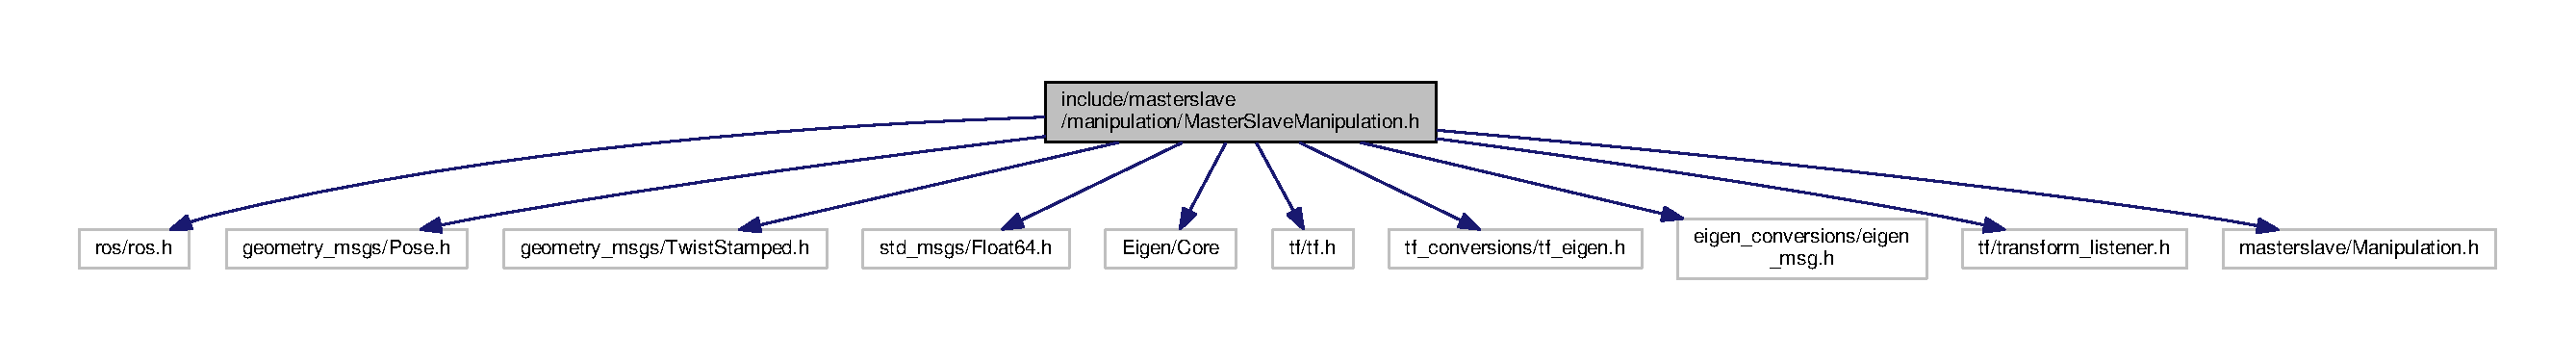
\includegraphics[width=350pt]{MasterSlaveManipulation_8h__incl}
\end{center}
\end{figure}
\subsection*{Klassen}
\begin{DoxyCompactItemize}
\item 
class \hyperlink{classMasterSlaveManipulation}{Master\-Slave\-Manipulation}
\begin{DoxyCompactList}\small\item\em Klasse, die sich um die Manipulation des T\-C\-P mittels des Eingabegerätes kümmert. \end{DoxyCompactList}\end{DoxyCompactItemize}

\hypertarget{CircleTrajectory_8h}{\section{include/masterslave/manipulation/trajectory/\-Circle\-Trajectory.h-\/\-Dateireferenz}
\label{CircleTrajectory_8h}\index{include/masterslave/manipulation/trajectory/\-Circle\-Trajectory.\-h@{include/masterslave/manipulation/trajectory/\-Circle\-Trajectory.\-h}}
}
{\ttfamily \#include \char`\"{}I\-Trajectory.\-h\char`\"{}}\\*
{\ttfamily \#include \char`\"{}Eigen/\-Core\char`\"{}}\\*
{\ttfamily \#include \char`\"{}Eigen/\-Dense\char`\"{}}\\*
Include-\/\-Abhängigkeitsdiagramm für Circle\-Trajectory.\-h\-:
\nopagebreak
\begin{figure}[H]
\begin{center}
\leavevmode
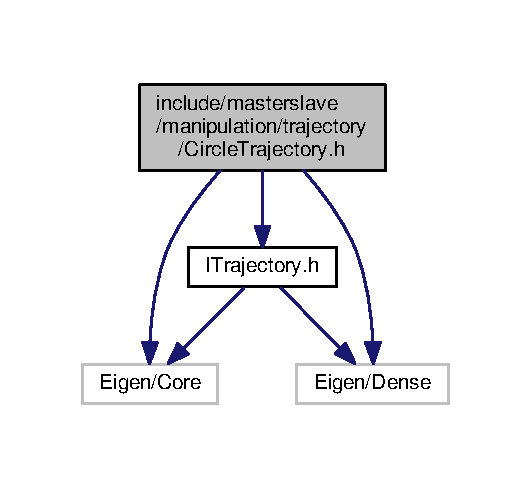
\includegraphics[width=255pt]{CircleTrajectory_8h__incl}
\end{center}
\end{figure}
Dieser Graph zeigt, welche Datei direkt oder indirekt diese Datei enthält\-:
\nopagebreak
\begin{figure}[H]
\begin{center}
\leavevmode
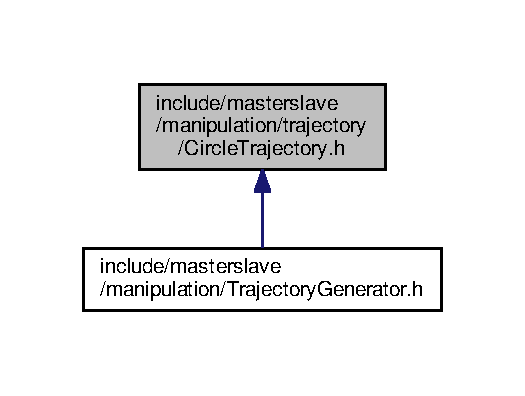
\includegraphics[width=252pt]{CircleTrajectory_8h__dep__incl}
\end{center}
\end{figure}
\subsection*{Klassen}
\begin{DoxyCompactItemize}
\item 
class \hyperlink{classCircleTrajectory}{Circle\-Trajectory}
\begin{DoxyCompactList}\small\item\em Klasse, die eine Interpolation einer Kreistrajektorie ermöglicht. \end{DoxyCompactList}\end{DoxyCompactItemize}

\hypertarget{ITrajectory_8h}{\section{include/masterslave/manipulation/trajectory/\-I\-Trajectory.h-\/\-Dateireferenz}
\label{ITrajectory_8h}\index{include/masterslave/manipulation/trajectory/\-I\-Trajectory.\-h@{include/masterslave/manipulation/trajectory/\-I\-Trajectory.\-h}}
}
{\ttfamily \#include \char`\"{}Eigen/\-Core\char`\"{}}\\*
{\ttfamily \#include \char`\"{}Eigen/\-Dense\char`\"{}}\\*
Include-\/\-Abhängigkeitsdiagramm für I\-Trajectory.\-h\-:
\nopagebreak
\begin{figure}[H]
\begin{center}
\leavevmode
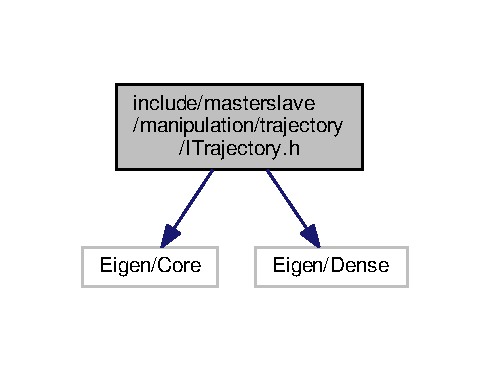
\includegraphics[width=235pt]{ITrajectory_8h__incl}
\end{center}
\end{figure}
Dieser Graph zeigt, welche Datei direkt oder indirekt diese Datei enthält\-:
\nopagebreak
\begin{figure}[H]
\begin{center}
\leavevmode
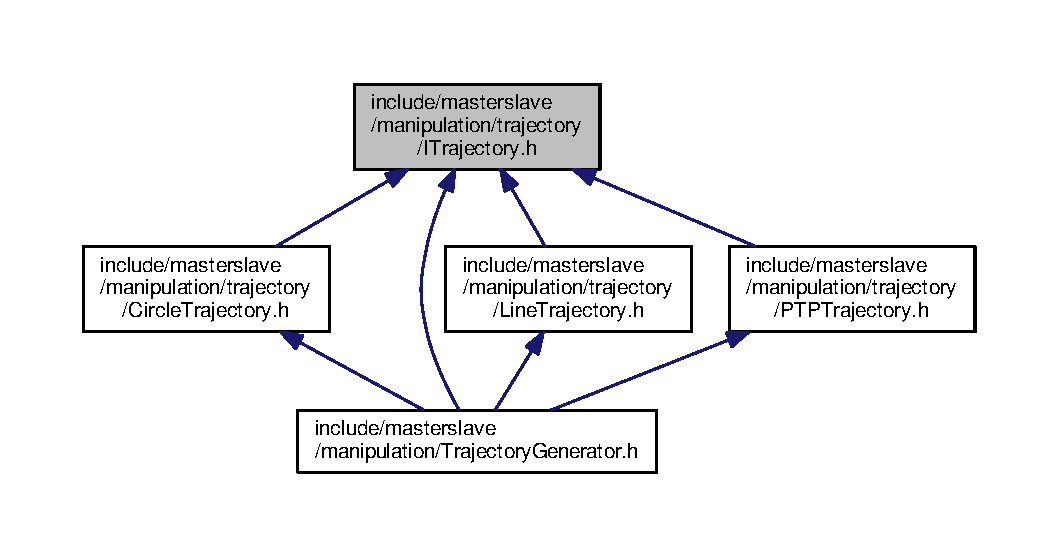
\includegraphics[width=350pt]{ITrajectory_8h__dep__incl}
\end{center}
\end{figure}
\subsection*{Klassen}
\begin{DoxyCompactItemize}
\item 
class \hyperlink{classITrajectory}{I\-Trajectory}
\begin{DoxyCompactList}\small\item\em Abstrakte Basisklasse für verschiedene Trajektorienarten. \end{DoxyCompactList}\end{DoxyCompactItemize}

\hypertarget{LineTrajectory_8h}{\section{include/masterslave/manipulation/trajectory/\-Line\-Trajectory.h-\/\-Dateireferenz}
\label{LineTrajectory_8h}\index{include/masterslave/manipulation/trajectory/\-Line\-Trajectory.\-h@{include/masterslave/manipulation/trajectory/\-Line\-Trajectory.\-h}}
}
{\ttfamily \#include \char`\"{}I\-Trajectory.\-h\char`\"{}}\\*
{\ttfamily \#include $<$array$>$}\\*
Include-\/\-Abhängigkeitsdiagramm für Line\-Trajectory.\-h\-:
\nopagebreak
\begin{figure}[H]
\begin{center}
\leavevmode
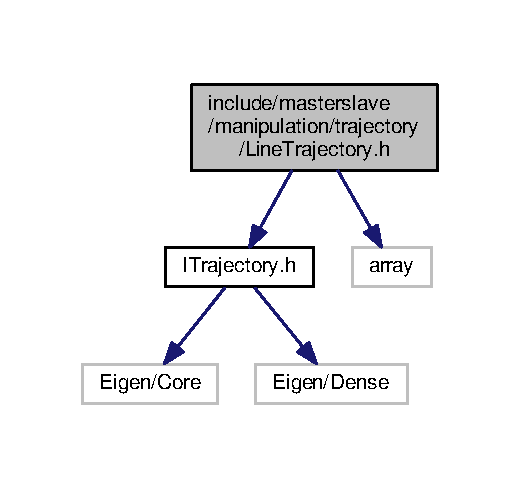
\includegraphics[width=250pt]{LineTrajectory_8h__incl}
\end{center}
\end{figure}
Dieser Graph zeigt, welche Datei direkt oder indirekt diese Datei enthält\-:
\nopagebreak
\begin{figure}[H]
\begin{center}
\leavevmode
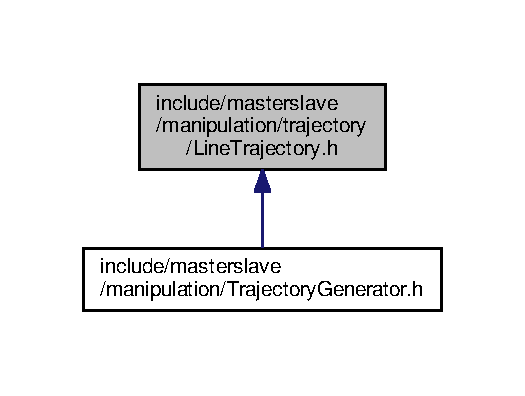
\includegraphics[width=252pt]{LineTrajectory_8h__dep__incl}
\end{center}
\end{figure}
\subsection*{Klassen}
\begin{DoxyCompactItemize}
\item 
class \hyperlink{classLineTrajectory}{Line\-Trajectory}
\begin{DoxyCompactList}\small\item\em Eine Klasse, die eine Interpolation eines Polynom fünften Grades zwischen zwei Punkten ermöglicht. \end{DoxyCompactList}\end{DoxyCompactItemize}

\hypertarget{TrajectoryGenerator_8h}{\section{include/masterslave/manipulation/\-Trajectory\-Generator.h-\/\-Dateireferenz}
\label{TrajectoryGenerator_8h}\index{include/masterslave/manipulation/\-Trajectory\-Generator.\-h@{include/masterslave/manipulation/\-Trajectory\-Generator.\-h}}
}
{\ttfamily \#include \char`\"{}ros/ros.\-h\char`\"{}}\\*
{\ttfamily \#include \char`\"{}masterslave/\-Manipulation.\-h\char`\"{}}\\*
{\ttfamily \#include \char`\"{}geometry\-\_\-msgs/\-Pose.\-h\char`\"{}}\\*
{\ttfamily \#include \char`\"{}geometry\-\_\-msgs/\-Twist\-Stamped.\-h\char`\"{}}\\*
{\ttfamily \#include \char`\"{}std\-\_\-msgs/\-Float64.\-h\char`\"{}}\\*
{\ttfamily \#include \char`\"{}Eigen/\-Core\char`\"{}}\\*
{\ttfamily \#include $<$tf/tf.\-h$>$}\\*
{\ttfamily \#include $<$tf\-\_\-conversions/tf\-\_\-eigen.\-h$>$}\\*
{\ttfamily \#include $<$eigen\-\_\-conversions/eigen\-\_\-msg.\-h$>$}\\*
{\ttfamily \#include $<$tf/transform\-\_\-listener.\-h$>$}\\*
{\ttfamily \#include \char`\"{}masterslave/manipulation/trajectory/\-Line\-Trajectory.\-h\char`\"{}}\\*
{\ttfamily \#include \char`\"{}masterslave/manipulation/trajectory/\-P\-T\-P\-Trajectory.\-h\char`\"{}}\\*
{\ttfamily \#include \char`\"{}masterslave/manipulation/trajectory/\-Circle\-Trajectory.\-h\char`\"{}}\\*
{\ttfamily \#include \char`\"{}masterslave/manipulation/trajectory/\-I\-Trajectory.\-h\char`\"{}}\\*
{\ttfamily \#include $<$dynamic\-\_\-reconfigure/server.\-h$>$}\\*
{\ttfamily \#include \char`\"{}masterslave/\-Trajectory\-Generator\-Config.\-h\char`\"{}}\\*
Include-\/\-Abhängigkeitsdiagramm für Trajectory\-Generator.\-h\-:
\nopagebreak
\begin{figure}[H]
\begin{center}
\leavevmode
\includegraphics[width=350pt]{TrajectoryGenerator_8h__incl}
\end{center}
\end{figure}
\subsection*{Klassen}
\begin{DoxyCompactItemize}
\item 
class \hyperlink{classTrajectoryGenerator}{Trajectory\-Generator}
\begin{DoxyCompactList}\small\item\em Klasse zum Abfahren verschiedener Trajektorien zur quantitativen Bestimmung des Trokarpunktes. \end{DoxyCompactList}\end{DoxyCompactItemize}
\subsection*{Aufzählungen}
\begin{DoxyCompactItemize}
\item 
enum \hyperlink{TrajectoryGenerator_8h_ab7e9971a19ca76371c40959c478f6618}{T\-R\-A\-J\-E\-C\-T\-O\-R\-Y\-\_\-\-S\-T\-A\-T\-E} \{ {\bfseries N\-O\-\_\-\-S\-T\-A\-T\-E} = -\/1, 
{\bfseries P\-T\-P}, 
{\bfseries L\-I\-N\-E}, 
{\bfseries C\-I\-R\-C\-L\-E}
 \}
\begin{DoxyCompactList}\small\item\em Verschiedene Trajektorienarten, die die Klassen \hyperlink{classTrajectoryGenerator}{Trajectory\-Generator} zur Verfügung stellt. \end{DoxyCompactList}\end{DoxyCompactItemize}


\subsection{Dokumentation der Aufzählungstypen}
\hypertarget{TrajectoryGenerator_8h_ab7e9971a19ca76371c40959c478f6618}{\index{Trajectory\-Generator.\-h@{Trajectory\-Generator.\-h}!T\-R\-A\-J\-E\-C\-T\-O\-R\-Y\-\_\-\-S\-T\-A\-T\-E@{T\-R\-A\-J\-E\-C\-T\-O\-R\-Y\-\_\-\-S\-T\-A\-T\-E}}
\index{T\-R\-A\-J\-E\-C\-T\-O\-R\-Y\-\_\-\-S\-T\-A\-T\-E@{T\-R\-A\-J\-E\-C\-T\-O\-R\-Y\-\_\-\-S\-T\-A\-T\-E}!TrajectoryGenerator.h@{Trajectory\-Generator.\-h}}
\subsubsection[{T\-R\-A\-J\-E\-C\-T\-O\-R\-Y\-\_\-\-S\-T\-A\-T\-E}]{\setlength{\rightskip}{0pt plus 5cm}enum {\bf T\-R\-A\-J\-E\-C\-T\-O\-R\-Y\-\_\-\-S\-T\-A\-T\-E}}}\label{TrajectoryGenerator_8h_ab7e9971a19ca76371c40959c478f6618}


Verschiedene Trajektorienarten, die die Klassen \hyperlink{classTrajectoryGenerator}{Trajectory\-Generator} zur Verfügung stellt. 

\begin{DoxySeeAlso}{Siehe auch}
\hyperlink{classTrajectoryGenerator}{Trajectory\-Generator} 
\end{DoxySeeAlso}

\hypertarget{RosOpenIGTLBridge_8h}{\section{include/masterslave/\-Ros\-Open\-I\-G\-T\-L\-Bridge.h-\/\-Dateireferenz}
\label{RosOpenIGTLBridge_8h}\index{include/masterslave/\-Ros\-Open\-I\-G\-T\-L\-Bridge.\-h@{include/masterslave/\-Ros\-Open\-I\-G\-T\-L\-Bridge.\-h}}
}
{\ttfamily \#include $<$ros/ros.\-h$>$}\\*
{\ttfamily \#include $<$stdlib.\-h$>$}\\*
{\ttfamily \#include \char`\"{}geometry\-\_\-msgs/\-Pose\-Stamped.\-h\char`\"{}}\\*
{\ttfamily \#include \char`\"{}geometry\-\_\-msgs/\-Pose\-Array.\-h\char`\"{}}\\*
{\ttfamily \#include \char`\"{}std\-\_\-msgs/\-Float64.\-h\char`\"{}}\\*
{\ttfamily \#include \char`\"{}sensor\-\_\-msgs/\-Joint\-State.\-h\char`\"{}}\\*
{\ttfamily \#include $<$dynamic\-\_\-reconfigure/server.\-h$>$}\\*
{\ttfamily \#include $<$masterslave/\-Ros\-Open\-I\-G\-T\-L\-Bridge\-Config.\-h$>$}\\*
{\ttfamily \#include \char`\"{}masterslave/\-Open\-I\-G\-T\-L\-State\-Description.\-h\char`\"{}}\\*
{\ttfamily \#include \char`\"{}masterslave/\-Open\-I\-G\-T\-L\-State\-Service.\-h\char`\"{}}\\*
{\ttfamily \#include \char`\"{}ros/callback\-\_\-queue.\-h\char`\"{}}\\*
{\ttfamily \#include $<$boost/bind.\-hpp$>$}\\*
{\ttfamily \#include $<$boost/thread.\-hpp$>$}\\*
{\ttfamily \#include \char`\"{}boost/thread/mutex.\-hpp\char`\"{}}\\*
{\ttfamily \#include \char`\"{}igtl\-O\-S\-Util.\-h\char`\"{}}\\*
{\ttfamily \#include \char`\"{}igtl\-Message\-Header.\-h\char`\"{}}\\*
{\ttfamily \#include \char`\"{}igtl\-Transform\-Message.\-h\char`\"{}}\\*
{\ttfamily \#include \char`\"{}igtl\-Client\-Socket.\-h\char`\"{}}\\*
{\ttfamily \#include \char`\"{}igtl\-Status\-Message.\-h\char`\"{}}\\*
{\ttfamily \#include \char`\"{}igtl\-String\-Message.\-h\char`\"{}}\\*
{\ttfamily \#include \char`\"{}igtl\-\_\-transform.\-h\char`\"{}}\\*
{\ttfamily \#include $<$sstream$>$}\\*
{\ttfamily \#include \char`\"{}Eigen/\-Eigen\char`\"{}}\\*
{\ttfamily \#include \char`\"{}Eigen/\-Dense\char`\"{}}\\*
{\ttfamily \#include $<$eigen\-\_\-conversions/eigen\-\_\-msg.\-h$>$}\\*
Include-\/\-Abhängigkeitsdiagramm für Ros\-Open\-I\-G\-T\-L\-Bridge.\-h\-:
\nopagebreak
\begin{figure}[H]
\begin{center}
\leavevmode
\includegraphics[width=350pt]{RosOpenIGTLBridge_8h__incl}
\end{center}
\end{figure}
\subsection*{Klassen}
\begin{DoxyCompactItemize}
\item 
class \hyperlink{classRosOpenIgtlBridge}{Ros\-Open\-Igtl\-Bridge}
\begin{DoxyCompactList}\small\item\em Eine R\-O\-S-\/\-Node zur Kommunikation zwischen R\-O\-S und dem L\-B\-R iiwa, welche über das Open\-I\-G\-T\-Link-\/\-Protokoll durchgeführt. \end{DoxyCompactList}\end{DoxyCompactItemize}

%--- End generated contents ---

% Index
\newpage
\phantomsection
\addcontentsline{toc}{chapter}{Index}
\printindex

\end{document}
